\documentclass[12pt,openany,makeidx]{book}

\usepackage{times}
\usepackage{amsmath,amssymb,amsthm}

\usepackage{makeidx}
\makeindex

\usepackage[hyperindex]{hyperref}
%\usepackage{chappg}

%\numberwithin{page}{chapter}
%\renewcommand{\thepage}{\arabic{chapter}-\arabic{page}}
%\let\oldchapter=\chapter
%\def\resetpage{\setcounter{page}{1}}
%\def\chapter{\expandafter\resetpage\oldchapter}


\topmargin         -0.25in
\oddsidemargin      0.5in
\evensidemargin     0.5in
\textheight         8.5in
\textwidth          5.5in

\iftrue
\newtheorem{theorem}{Theorem}[section]
\newtheorem{corollary}[theorem]{Corollary}
\newtheorem{definition}[theorem]{Definition}
\newtheorem{fact}[theorem]{Fact}
\newtheorem{lemma}[theorem]{Lemma}
\newtheorem{example}[theorem]{Example}
\newtheorem{problem}[theorem]{P}
\newtheorem{solution}[theorem]{S}
\else
\newtheorem{theorem}{Theorem}
\newtheorem{corollary}{Corollary}
\newtheorem{definition}{Definition}
\newtheorem{fact}{Fact}
\newtheorem{lemma}{Lemma}
\newtheorem{example}{Example}
\newtheorem{problem}{P}
\newtheorem{solution}{S}
\fi

\newcommand{\Interior}[1]{\ensuremath{{#1}^{\circ}}}
\newcommand{\Closure}[1]{\ensuremath{\overline{#1}}}
\newcommand{\Complement}[1]{\ensuremath{{#1}^{c}}}

\newcommand{\Expect}{\ensuremath{\mathrm{E}}}
\newcommand{\vecnot}{\underline}
\newcommand{\RealNumbers}{\mathbb{R}}
\newcommand{\RationalNumbers}{\mathbb{Q}}
\newcommand{\ComplexNumbers}{\mathbb{C}}
\newcommand{\Real}{\mathrm{Re}}
\newcommand{\Span}{\mathrm{span}}
\newcommand{\Rank}{\mathrm{rank}}
\newcommand{\Nullity}{\mathrm{nullity}}
\newcommand{\Trace}{\mathrm{tr}}
\newcommand{\Diag}{\mathrm{diag}}
\DeclareMathOperator{\esssup}{esssup}

%% Definitions
%%
\renewcommand{\baselinestretch}{1.25}
\newcommand{\defn}[2]{\textbf{\textrm{#2}}\index{#1!#2}}


\begin{document}

\frontmatter 

%\author{Major Contributors \\ Jean-Francois Chamberland and Henry D. Pfister} 
\title{Engineering Fundamentals} 
\date{November 20th, 2009} 

\maketitle

\iffalse

\chapter*{Copyright}
Copyright \copyright 2006-2008 by Jean-Francois Chamberland

Permission is granted to copy, distribute and/or modify this document under the terms of the \emph{GNU Free Documentation License}, Version 1.2 or any later version published by the \emph{Free Software Foundation}; with no Invariant Sections, no Front-Cover Texts, and no Back-Cover Texts.
A copy of the license is included in the section entitled ``GNU Free Documentation License''.
\fi

\tableofcontents 
%\chapter*{Preface}

This book is an outgrowth of a first year graduate course for engineers
that aims to develop intuition and analaysis in general linear spaces.
It is also intended to start graduate students on the road to mathematical
maturity.

The ideas are divided into three main parts:

Both engineering intuition and facility with writing proofs can be developed with practice.

Proofs are used to validate intuitive ideas about engineering systems.

Like music and art, theoretical engineering is learned by doing, not just by reading texts and listening to lectures.

Doing the exercises is the best way to get a feel for the material, test your understanding and see what needs further study.
It is important that you try to do the exercises by yourself prior to discussing with other students or your instructor.
Once solved, problems often appear much easier than they really are.
Testing your knowledge during exams is a dangerous proposition.

In this book we decided to take a good thing and make it better, adding the symbol $\triangle$ to the end of a definition, the symbol $\diamond$ for the end of an example.

Physical sloppiness is often a sign of either laziness or disrespect, and sloppiness in writing style is often a mask for sloppy thinking.


Functional knowledge,
but can you prove it?

A statement is something that can be verified, it has to be either true or false.
We will be making two assumptions when dealing with statements: every statement is either true or false, and no statement is both true and false.
One of the consequences of this law is that if a statement is not false, then it must be true.
Hence, to prove that something is true, it would suffice to show that it is not false.

"Write a computer program."
"Eat a pineapple"

What makes statement valuable for our purposes is that there are a number of ways of forming new statements from old ones.

In literary writing, some measure of ambiguity is often acceptable, and sometime valuable.
In mathematics, by contrast, precision is key; ambiguity is to be avoided at all cost.
When using a mathematical term, always stick to the precise mathematical definition, regardless of any other colloquial usage.



 

\mainmatter 

%\setcounter{chapter}{-1}
\chapter{Logic and Set Theory}


\begin{quote}
To criticize mathematics for its abstraction is to miss the point entirely.
Abstraction is what makes mathematics work.
If you concentrate too closely on too limited an application of a mathematical idea, you rob the mathematician of his most important tools: analogy, generality, and simplicity.
\flushright{\textit{-- Ian Stewart} \\ Does God play dice? The mathematics of chaos}
\end{quote}

\index{logic}

In mathematics, a \defn{logic}{proof} is a demonstration that, assuming certain axioms, some statement is necessarily true.
That is, a proof is a logical argument, not an empirical one.
One must demonstrate that a proposition is true in all cases before it is considered a theorem of mathematics.
An unproven proposition for which there is some sort of empirical evidence is known as a \defn{logic}{conjecture}.
Mathematical logic is the framework upon which rigorous proofs are built.
It is the study of the principles and criteria of valid inference and demonstrations.

Logicians have analyzed set theory in great details, formulating a collection of axioms that affords a broad enough and strong enough foundation to mathematical reasoning.
The standard form of axiomatic set theory is the Zermelo-Fraenkel set theory, together with the axiom of choice.
Each of the axioms included in this theory expresses a property of sets that is widely accepted by mathematicians.
It is unfortunately true that careless use of set theory can lead to contradictions.
Avoiding such contradictions was one of the original motivations for the axiomatization of set theory.

A rigorous analysis of set theory belongs to the foundations of mathematics and mathematical logic.
The study of these topics is, in itself, a formidable task.
For our purposes, it will suffice to approach basic logical concepts informally.
That is, we adopt a naive point of view regarding set theory and assume that the meaning of a set as a collection of objects is intuitively clear.
While informal logic is not itself rigorous, it provides the underpinning for rigorous proofs.
The rules we follow in dealing with sets are derived from established axioms.
At some point of your academic career, you may wish to study set theory and logic in greater detail.
Our main purpose here is to learn how to state mathematical results clearly and how to prove them.


\section{Statements}

A proof in mathematics demonstrates the truth of certain \textbf{statement}.
It is therefore natural to begin with a brief discussion of statements.
A statement, or \textbf{proposition}, is the content of an assertion.
It is either true or false, but cannot be both true and false at the same time.
For example, the expression ``There are no classes at Texas A\&M University today'' is a statement since it is either true or false.
The expression ``Do not cheat and do not tolerate those who do'' is not a statement.
Note that an expression being a statement does not depend on whether we personally can verify its validity.
The expression ``The base of the natural logarithm, denoted $e$, is an irrational number'' is a statement that most of us cannot prove.

Statements on their own are fairly uninteresting.
What brings value to logic is the fact that there are a number of ways to form new statements from old ones.
In this section, we present five ways to form new statements from old ones.
They correspond to the English expressions: and; or; not; if, then; if and only if.
In the discussion below, $P$ and $Q$ represent two abstract statements.

A logical \defn{logic}{conjunction} is an operation on two logical propositions that produces a value of true if both statements are true, and is false otherwise.
The conjunction (or logical AND) of $P$ and $Q$, denoted by $P \wedge Q$, is precisely defined by
\begin{center}
\begin{tabular}{|c|c|c|}
\hline
$P$ & $Q$ & $P \wedge Q$ \\
\hline
T & T & T \\
T & F & F \\
F & T & F \\
F & F & F \\
\hline
\end{tabular} .
\end{center}

Similarly, a logical \defn{logic}{disjunction} is an operator on two logical propositions that is true if either statements is true or both are true, and is false otherwise.
The disjunction (or logical OR) of $P$ and $Q$, denoted $P \vee Q$, is defined by
\begin{center}
\begin{tabular}{|c|c|c|}
\hline
$P$ & $Q$ & $P \vee Q$ \\
\hline
T & T & T \\
T & F & T \\
F & T & T \\
F & F & F \\
\hline
\end{tabular} .
\end{center}

In mathematics, a \defn{logic}{negation} is an operator on the logical value of a proposition that sends true to false and false to true.
The negation (or logical NOT) of $P$, denoted $\neg P$, is given by
\begin{center}
\begin{tabular}{|c|c|}
\hline
$P$ & $\neg P$ \\
\hline
T & F \\
F & T \\
\hline
\end{tabular} .
\end{center}

The next method of combining mathematical statements is slightly more subtle than the preceding ones.
It is connected to the notion of logical implication.
The \defn{logic}{conditional} from $P$ to $Q$, denoted $P \rightarrow Q$, is mathematically true if it is not the case that $P$ is true and $Q$ is false.
The precise definition of $P \rightarrow Q$ is given in the truth table
\begin{center}
\begin{tabular}{|c|c|c|}
\hline
$P$ & $Q$ & $P \rightarrow Q$ \\
\hline
T & T & T \\
T & F & F \\
F & T & T \\
F & F & T \\
\hline
\end{tabular} .
\end{center}
This table should match your intuition when $P$ is true.
When $P$ is false, students often think the resulting truth value should be undefined.
Although it may seem strange at first glance, this truth table is universally accepted by mathematicians.
To motivate this definition, one can think of $P \rightarrow Q$ as a promise that $Q$ is true whenever $P$ is true.
When $P$ is false, the promise is kept by default.
This definition allows one to combine many statements together and detect broken promises without being distracted by uninformative statements.

Logicians draw a firm distinction between the \defn{logic}{conditional connective} and the \defn{logic}{implication relation}.
They use the phrase ``if $P$ then $Q$'' for the conditional connective and the phrase ``$P$ implies $Q$'' for the implication relation.
They explain the difference between these two forms by saying that the conditional is the contemplated relation, while the implication is the asserted relation.
We will discuss this distinction in the Section~\ref{section:Relations}, where we formally study relations between statements.
The importance and soundness of the conditional form $P \rightarrow Q$ will become clearer then.

The logical \defn{logic}{biconditional} is an operator connecting two logical propositions that is true if the statements are both true or both false, and it is false otherwise.
The biconditional from $P$ to $Q$, denoted $P \leftrightarrow Q$, is precisely defined by
\begin{center}
\begin{tabular}{|c|c|c|}
\hline
$P$ & $Q$ & $P \leftrightarrow Q$ \\
\hline
T & T & T \\
T & F & F \\
F & T & F \\
F & F & T \\
\hline
\end{tabular} .
\end{center}
We read $P \leftrightarrow Q$ as ``$P$ if and only if $Q$.''
The phrase ``if and only if'' is often abbreviated as ``iff''.

Using the five basic operations defined above, it is possible to form more complicated compound statements.
We sometimes need parentheses to avoid ambiguity in writing compound statements.
We use the convention that $\neg$ takes precedence over the other four operations, but none of these operations takes precedence over the others.
For example, let $P$, $Q$ and $R$ be three propositions.
We wish to make a truth table for the following statement,
\begin{equation} \label{equation:LogicStatement}
(P \rightarrow R) \wedge (Q \vee \neg R) .
\end{equation}
We can form the true table for this statement, using simple steps, as follows
\begin{center}
\begin{tabular}{|c|c|c|ccccccc|}
\hline
$P$ & $Q$ & $R$
& $(P$ & $\rightarrow$ & $R)$ & $\wedge$ & $(Q$ & $\vee$ & $\neg R)$ \\
\hline
T & T & T & T & T & T & T & T & T & F \\
T & T & F & T & F & F & F & T & T & T \\
T & F & T & T & T & T & F & F & F & F \\
T & F & F & T & F & F & F & F & T & T \\
F & T & T & F & T & T & T & T & T & F \\
F & T & F & F & T & F & T & T & T & T \\
F & F & T & F & T & T & F & F & F & F \\
F & F & F & F & T & F & T & F & T & T \\
& & & 1 & 5 & 2 & 7 & 3 & 6 & 4 \\
\hline
\end{tabular} .
\end{center}
%\end{example}

We conclude this section with a brief mention of two important concepts.
A \defn{logic}{tautology} is a statement that is true in every valuation of its propositional variables, independent of the truth values assigned to these variables.
The proverbial tautology is $P \vee \neg P$,
\begin{center}
\begin{tabular}{|c|ccc|}
\hline
$P$ & $P$ & $\vee$ & $\neg P$ \\
\hline
T & T & T & F \\
F & F & T & T \\
& 1 & 3 & 2 \\
\hline
\end{tabular} .
\end{center}
For instance, the statement ``The Aggies won their last football game or the Aggies did not win their last football game'' is true regardless of whether the Aggies actually defeated their latest opponent.

The negation of a tautology is a \defn{logic}{contradiction}, a statement that is necessarily false regardless of the truth values of its propositional variables.
The statement $P \wedge \neg P$ is a contradiction, and its truth table is
\begin{center}
\begin{tabular}{|c|ccc|}
\hline
$P$ & $P$ & $\wedge$ & $\neg P$ \\
\hline
T & T & F & F \\
F & F & F & T \\
& 1 & 3 & 2 \\
\hline
\end{tabular} .
\end{center}

Of course, most statement we encounter are neither tautologies nor contradictions.
For example, \eqref{equation:LogicStatement} is not necessarily either true or false.
Its truth value depends on the values of $P$, $Q$ and $R$.
Try to see whether the statement
\begin{equation*}
((P \wedge Q) \rightarrow R) \rightarrow (P \rightarrow (Q \rightarrow R))
\end{equation*}
is a tautology, a contradiction, or neither.


\section{Relations between Statements}
\label{section:Relations}

Strictly speaking, relations between statements are not formal statements themselves.
They are \emph{meta-statements} about some propositions.
We study two types of relations between statements, \emph{implication} and \emph{equivalence}.
An example of an implication meta-statement is the observation that ``if the statement `Robert graduated from Texas A\&M University' is true, then it implies that the statement `Robert is an Aggie' is also true.''
Another example of a meta-statement is ``the statement `Fred is an Aggie and Fred is honest' being true is equivalent to the statement `Fred is honest and Fred is an Aggie' being true.''
These two examples illustrate how meta-statements describe the relationship between statements.
It is also instructive to note that implications and equivalences are the meta-statement analogs of conditionals and biconditionals.

A \defn{logic}{logical implication} can be intuitively described as $P$ implies $Q$ if $Q$ must be true whenever $P$ is true.
That is, $Q$ cannot be false if $P$ is true.
Necessity is the key aspect of this sentence, the fact that $P$ and $Q$ both happen to be true cannot be coincidental.
To have $P$ implies $Q$, we need the conditional $P \rightarrow Q$ to be true under all possible circumstances.

The notion of implication can be rigorously defined as follows, $P$ implies $Q$ if the statement $P \rightarrow Q$ is a tautology.
We abbreviate $P$ implies $Q$ by writing $P \Rightarrow Q$.
It is important to understand the difference between ``$P \rightarrow Q$'' and ``$P \Rightarrow Q$.''
The former, $P \rightarrow Q$, is a compound statement that may or may not be true.
On the other hand, $P \Rightarrow Q$ is a relation stating that the compound statement $P \rightarrow Q$ is true under all instances of $P$ and $Q$.

While the distinction between implication and conditional may seem extraneous, we will soon see that meta-statements become extremely useful in building valid arguments.
In particular, the following implications are used extensively in constructing proofs.
\begin{fact}
Let $P$, $Q$, $R$ and $S$ be statements.
\begin{enumerate}
\item $(P \rightarrow Q) \wedge P \Rightarrow Q$.
\item $(P \rightarrow Q) \wedge \neg Q \Rightarrow \neg P$.
\item $P \wedge Q \Rightarrow P$.
\item $(P \vee Q) \wedge \neg P \Rightarrow Q$.
\item $P \leftrightarrow Q \Rightarrow P \rightarrow Q$.
\item $(P \rightarrow Q) \wedge (Q \rightarrow P) \Rightarrow P \rightarrow Q$.
\item $(P \rightarrow Q) \wedge (Q \rightarrow R) \Rightarrow P \rightarrow R$
\item $(P \rightarrow Q) \wedge (R \rightarrow S) \wedge (P \vee R) \Rightarrow Q \vee S$.
\end{enumerate}
\end{fact}

As an illustrative example, we show that $(P \rightarrow Q) \wedge (Q \rightarrow R)$ implies $P \rightarrow R$.
To demonstrate this assertion, we need to show that
\begin{equation} \label{equation:HypotheticalSyllogism}
((P \rightarrow Q) \wedge (Q \rightarrow R)) \rightarrow (P \rightarrow R)
\end{equation}
is a tautology.
This is accomplished in the truth table below
\begin{center}
\begin{tabular}{|c|c|c|ccccccccccc|}
\hline
$P$ & $Q$ & $R$
& $((P$ & $\rightarrow$ & $Q)$ & $\wedge$ & $(Q$ & $\rightarrow$ & $R))$ & $\rightarrow$ & $(P$ & $\rightarrow$ & $R)$ \\
\hline
T & T & T & T & T & T & T & T & T & T & T & T & T & T \\
T & T & F & T & T & T & F & T & F & F & T & T & F & F \\
T & F & T & T & F & F & F & F & T & T & T & T & T & T \\
T & F & F & T & F & F & F & F & T & F & T & T & F & F \\
F & T & T & F & T & T & T & T & T & T & T & F & T & T \\
F & T & F & F & T & T & F & T & F & F & T & F & T & F \\
F & F & T & F & T & F & T & F & T & T & T & F & T & T \\
F & F & F & F & T & F & T & F & T & F & T & F & T & F \\
& & & 1 & 7 & 2 & 10 & 3 & 8 & 4 & 11 & 5 & 9 & 6 \\
\hline
\end{tabular} .
\end{center}
Column~11 has the truth values for statement \eqref{equation:HypotheticalSyllogism}.
Since \eqref{equation:HypotheticalSyllogism} is true under all circumstances, it is a tautology and the implication holds.
Showing that the other relations are valid is left to the reader as an exercise.

Reversing the arrow in a conditional statement gives the \defn{logic}{converse} of that statement.
For example, the statement $Q \rightarrow P$ is the converse of $P \rightarrow Q$.
This reversal may not preserve the truth of the statement though and therefore logical implications are not always reversible.
For instance, although $(P \rightarrow Q) \wedge (Q \rightarrow R)$ implies $P \rightarrow R$, the converse is not always true.
It can easily be seen from columns~9~\&~10 above that
\begin{equation*}
(P \rightarrow R) \rightarrow ((P \rightarrow Q) \wedge (Q \rightarrow R))
\end{equation*}
is not a tautology.
That is, $P \rightarrow R$ certainly does not imply $(P \rightarrow Q) \wedge (Q \rightarrow R)$.

A logical implication that is reversible is called a \defn{logic}{logical equivalence}.
More precisely, $P$ is equivalent to $Q$ if the statement $P \leftrightarrow Q$ is a tautology.
We denote the sentence ``$P$ is equivalent to $Q$'' by simply writing ``$P \Leftrightarrow Q$.''
The meta-statement $P \Leftrightarrow Q$ holds if and only if $P \Rightarrow Q$ and $Q \Rightarrow P$ are both true.
Being able to recognize that two statements are equivalent will become handy.
It is sometime possible to demonstrate a result by finding an alternative, equivalent form of the statement that is easier to prove than the original form.
A list of important equivalences appears below.

\begin{fact}
Let $P$, $Q$ and $R$ be statements.
\begin{enumerate}
\item $\neg (\neg P) \Leftrightarrow P$.
\item $P \vee Q \Leftrightarrow Q \vee P$.
\item $P \wedge Q \Leftrightarrow Q \wedge P$.
\item $(P \vee Q) \vee R \Leftrightarrow P \vee (Q \vee R)$.
\item $(P \wedge Q) \wedge R \Leftrightarrow P \wedge (Q \wedge R)$.
\item $P \wedge (Q \vee R) \Leftrightarrow (P \wedge Q) \vee (P \wedge R)$.
\item $P \vee (Q \wedge R) \Leftrightarrow (P \vee Q) \wedge (P \vee R)$.
\item $P \rightarrow Q \Leftrightarrow \neg P \vee Q$.
\item $P \rightarrow Q \Leftrightarrow \neg Q \rightarrow \neg P$ (Contrapositive).
\item $P \leftrightarrow Q \Leftrightarrow (P \rightarrow Q) \wedge (Q \rightarrow P)$.
\item $\neg (P \wedge Q) \Leftrightarrow \neg P \vee \neg Q$ (De Morgan's Law).
\item $\neg (P \vee Q) \Leftrightarrow \neg P \wedge \neg Q$ (De Morgan's Law).
\end{enumerate}
\end{fact}

The first equivalence in this list, $\neg (\neg P) \Leftrightarrow P$, may appear trivial.
However, from the point of view of constructing mathematical proofs, this equivalence is frequently employed.
Indeed, one method to prove that statement $P$ is true is to hypothesize that $\neg P$ is true and then derive a contradiction.
It then follows that $\neg P$ is false, which implies that $P$ is true.
This popular technique is called \defn{logic}{proof by contradiction}.
It is illustrated below through a classic example.

Given a conditional statement of the form $P \rightarrow Q$, we call $\neg Q \rightarrow \neg P$ the \defn{logic}{contrapositive} of the original statement.
The equivalence $P \rightarrow Q \Leftrightarrow \neg Q \rightarrow \neg P$ is also used extensively in constructing mathematical proofs.


\subsection{Fallacious Arguments}

A \defn{logic}{fallacy} is a component of an argument that is demonstrably flawed in its logic or form, thus rendering the argument invalid.
Recognizing fallacies in mathematical proofs may be difficult since arguments are often structured using convoluted patterns that obscure the logical connections between assertions.
We give below examples for three types of fallacies that are often found in attempted mathematical proofs.

\paragraph{Affirming the Consequent:}
If the Indian cricket team wins a test match, then all the players will drink tea together.
All the players drank tea together.
Therefore the Indian cricket team won a test match.

\paragraph{Denying the Antecedent:}
If Diego Maradona drinks coffee, then he will be fidgety.
Diego Maradona did not drink coffee.
Therefore, he is not fidgety.

\paragraph{Unwarranted Assumptions:}
If Yao Ming gets close to the basket, then he scores a lot of points.
Therefore, Yao Ming scores a lot of points.


\subsection{Quantifiers}

Quantifiers are of paramount importance in rigorous proofs.
They are employed to make statements about collections of elements.
Universal quantification is used to formalize the notion that a statement is true for all possible values of a collection.
The \defn{logic}{universal quantifier} is typically denoted by $\forall$ and it is informally read ``for all.''
Let $U$ be a specific collection of elements, and let $P(x)$ be a statement that applies to $x$.
Then the statement $\forall x \in U, P(x)$ is true if $P(x)$ is true for all values of $x$ in $U$.
The other type of quantifier often encountered in mathematical proofs is the \defn{logic}{existential quantifier}, denoted $\exists$.
The statement $\exists x \in U, P(x)$ is true if $P(x)$ is true for at least one value of $x$ in $U$.
Based on the meanings of the quantifiers, we have the following equivalences
\begin{gather*}
\neg \left( \left( \forall x \in U \right) P(x) \right)
\Leftrightarrow \left( \exists x \in U \right) \left( \neg P(x) \right) \\
\neg \left( \left( \exists x \in U \right) P(x) \right)
\Leftrightarrow \left( \forall x \in U \right) \left( \neg P(x) \right) .
\end{gather*}

In mathematics, a \textbf{free variable} is a notation for a place or places in an expression into which some definite substitution may take place, or with respect to which some operation (e.g. quantification) may take place. 
A \textbf{bound variable} is a variable for which we have no ability to choose the value.


\section{Strategies for Proofs}

The relation between intuition and formal rigor is not a trivial matter.
Intuition tells us what is important, what might be true, and what mathematical tools may be used to prove it.
Rigorous proofs are used to verify that a given statement that appears intuitively true is indeed true.
Ultimately, a mathematical proof is a convincing argument that starts from some premises, and logically deduces the desired conclusion.
Most proofs do not mention the logical rules of inference used in the derivation.
Rather, they focus on the mathematical justification of each step, leaving to the reader the task of filling the logical gaps.
The mathematics is the major issue.
Yet, it is essential that you understand the underlying logic behind the derivation as to not get confused while reading or writing a proof.

True statements in mathematics have different names.
They can be called theorems, propositions, lemmas, corollaries and exercises.
A \defn{logic}{theorem} is a statement that can be proved on the basis of explicitly stated or previously agreed assumptions.
A \defn{logic}{proposition} is a statement not associated with any particular theorem; this term sometimes connotes a statement with a simple proof.
A \defn{logic}{lemma} is a proven proposition which is used as a stepping stone to a larger result rather than an independent statement in itself.
A \defn{logic}{corollary} is a mathematical statement which follows easily from a previously proven statement, typically a mathematical theorem. 
The distinction between these names and their definitions is somewhat arbitrary.
Ultimately, they are all synonymous to a true statement.

A proof should be written in grammatically correct English.
Complete sentences should be used, with full punctuation.
In particular, every sentence should end with a period, even if the sentence ends in a displayed equation.
Mathematical formulas and symbols are parts of sentences, and are treated no differently than words.
One way to learn to construct proofs is to read a lot of well written proofs, to write progressively more difficult proofs, and to get detailed feedback on the proofs you write.


\paragraph{Direct Proof:}

The simplest form of proof for a statement of the form $P \rightarrow Q$ is the \textbf{direct proof}.
First assume that $P$ is true.
Produce a series of steps, each one following from the previous ones, that eventually leads to conclusion $Q$.
It warrants the name ``direct proof'' only to distinguish it from other, more intricate, methods of proof.

\paragraph{Proof by Contrapositive:}
A proof by contrapositive takes advantage of the mathematical equivalence $P \rightarrow Q \Leftrightarrow \neg Q \rightarrow \neg P$.
That is, a proof by contrapositive begins by assuming that $Q$ is false (i.e., $\neg Q$ is true).
It then produces a series of direct implications leading to the conclusion that $P$ is false (i.e., $\neg P$ is true).
It follows that $Q$ cannot be false when $P$ is true, so $P \rightarrow Q$.

\paragraph{Proof by Contradiction:}
A proof by contradiction is based on the mathematical equivalence $\neg (P \rightarrow Q) \Leftrightarrow P \wedge \neg Q$.
In a proof by contradiction, one starts by assuming that both $P$ and $\neg Q$ are true.
Then, a series of direct implications are given that lead to a logical contradiction.
Hence, $P \wedge \neg Q$ cannot be true and $P \rightarrow Q$.

\begin{example} \label{example:SquareRoot2}
We wish to show that $\sqrt{2}$ is an irrational number.

First, assume that $\sqrt{2}$ is a rational number.
This assumption implies that there exist integers $p$ and $q$ with $q \neq 0$ such that $p/q = \sqrt{2}$.
In fact, we can further assume that the fraction $p/q$ is irreducible.
That is, $p$ and $q$ are coprime integers (they have no common factor greater than 1).
From $p/q = \sqrt{2}$, it follows that $p = \sqrt{2} q$, and so $p^2 = 2 q^2$.
Thus $p^2$ is an even number, which implies that $p$ itself is even (only even numbers have even squares).
Because $p$ is even, there exists an integer $r$ satisfying $p = 2r$.
We then obtain the equation $(2r)^2 = 2q^2$, which is equivalent to $2r^2 = q^2$ after simplification.
Because $2r^2$ is even, it follows that $q^2$ is even, which means that $q$ is also even.
We conclude that $p$ and $q$ are both even.
This contradicts the fact that $p/q$ is irreducible.
Hence, the initial assumption that $\sqrt{2}$ is a rational number must be false.
That is to say, $\sqrt{2}$ is irrational.
\end{example}

\begin{example}
Consider the following statement, which is related to Example~\ref{example:SquareRoot2}.
``If $\sqrt{2}$ is rational, then it can be expressed as an irreducible fraction.''
The contrapositive of this statement is ``If $\sqrt{2}$ cannot be expressed as an irreducible fraction, then it is not rational.''
Above, we proved that $\sqrt{2}$ cannot be expressed as an irreducible fraction and therefore $\sqrt{2}$ is not a rational number.
\end{example}

\section{Set Theory}

Set theory is generally considered to be the foundation of all modern mathematics.
This means that most mathematical objects (numbers, relations, functions, etc.) are defined in terms of sets.
Unfortunately for engineers, set theory is not quite as simple as it seems.
It turns out that simple approaches to set theory include paradoxes (e.g., statements which are both true and false).
These paradoxes can be resolved by putting set theory in a firm axiomatic framework, but that exercise is rather unproductive for engineers.
Instead, we adopt what is called \defn{set theory}{naive set theory} which rigorously defines the operations of set theory without worrying about possible contradictions.
This approach is sufficient for most of mathematics and also acts as a stepping-stone to more formal treatments.

A \defn{set theory}{set} is any collection of objects, mathematical or otherwise.
For example, we can think of the set of all books published in 2007.
The objects in a set are referred to as \defn{set theory}{elements} or members of the set.
The logical statement ``$a$ is a member of the set $A$'' is written
\[ a \in A. \]
Likewise, its logical negation ``$a$ is not a member of the set $A$'' is written $a \notin A$.
Therefore, exactly one of these two statements is true.

One may present a set by listing its elements.
For example, $A= \{ a,e,i,o,u \}$ is the set of standard English vowels.
It is important to note that the order elements are presented is irrelevant and the set $\{ i,o,u,a,e \}$ is the same as $A$.
Likewise, repeated elements have no effect and the set $\{ a,e,i,o,u,e,o \}$ is the same as $A$.
A \defn{set theory}{singleton} set is a set containing exactly one element such as $\{a\}$.

There are a number of standard sets worth mentioning: the \defn{set theory}{integers} $\mathbb{Z}$, the \defn{set theory}{real numbers} $\mathbb{R}$, and the \defn{set theory}{complex numbers} $\mathbb{C}$.
It is possible to construct these sets in a rigorous manner, but instead we will assume their meaning is intuitively clear.
New sets can be defined in terms of old sets using \defn{set theory}{set-builder notation}.
Let $P(x)$ be a logical statement about objects $x$ in the set $X$, then the ``set of elements in $X$ such that $P(x)$ is true'' is denoted by
\[ \{ x\in X | P(x) \}. \]
For example, the set of even integers is given by
\[ \{ x\in \mathbb{Z} | \textrm{``}x\textrm{ is even''} \} = \{ \ldots,-4,-2,0,2,4,\ldots \}. \]
If no element $x\in X$ satisfies the condition, then the result is the \defn{set theory}{empty set} which is denoted $\emptyset$.
Using set-builder notation, we can also recreate the \defn{set theory}{natural numbers} $\mathbb{N}$ and the \defn{set theory}{rational numbers} $\mathbb{Q}$ with
\begin{align*}
\mathbb{N} & = \{ n\in \mathbb{Z} | n\geq 1 \} \\
\mathbb{Q} & = \{ q\in \mathbb{R} | q=a/b, a\in \mathbb{Z}, b\in \mathbb{N} \}.
\end{align*}
The following standard notation is used for interval subsets of the real numbers:
\begin{align*}
\textrm{Open interval:} \; &  (a,b) \triangleq \{ x\in \mathbb{R} | a<x<b \} \\
\textrm{Closed interval:} \; & [a,b] \;\;\!\! \triangleq \{ x\in \mathbb{R} | a \leq x \leq b \} \\
\textrm{Half-open intervals:} \; & (a,b] \;\! \triangleq \{ x\in \mathbb{R} | a < x \leq b \} \\
& [a,b) \;\! \triangleq \{ x\in \mathbb{R} | a \leq x < b \}
\end{align*}

\begin{example}[\defn{set theory}{Russell's Paradox}]
Let $R$ be the set of all sets that do not contain themselves or $R = \{S|S\notin S\}$.
The paradox arises from the fact that the definition implies the logical contradiction $R\in R \Leftrightarrow R\notin R$.
Axiomatic set theory eliminates this paradox by disallowing self-referencing constructions like this.
\end{example}

There are also some standard relations defined between any two sets $A,B$.
\begin{definition}
We say that $A$ \textbf{equals} $B$ (denoted $A=B$) if, for all $x$,  $x\in A$ iff $x\in B$.
This means that
\[ A=B \Leftrightarrow \forall x \left( (x\in A)\leftrightarrow (x\in B) \right). \]
\end{definition}

\begin{definition}
We say that $A$ is a \defn{set theory}{subset} of $B$ (denoted $A\subseteq B$) if, for all $x$, $x\in A$ implies $x\in B$.
This means that
\[ A\subseteq B  \Leftrightarrow \forall x \left( (x\in A)\rightarrow (x\in B) \right). \]
It is a \textbf{proper subset} (denoted $A\subset B$) if $A\subseteq B$ and $A\neq B$.
\end{definition}

There are also a number of operations between sets.
Let $A,B$ be any two sets.
\begin{definition}
The \defn{set theory}{union} of $A$ and $B$ (denoted $A\cup B$) is the set of elements in either $A$ or $B$.
This means that $A \cup B = \{ x\in A \textrm{ or } x\in B \}$ is also defined by
\[ x\in A\cup B \Leftrightarrow (x\in A)\vee (x\in B). \]
\end{definition}

\begin{definition}
The \defn{set theory}{intersection} of $A$ and $B$ (denoted $A\cap B$) is the set of elements in both $A$ and $B$.
This means that $A\cap B = \{x\in A | x\in B \}$ is also defined by
\[ x\in A\cap B \Leftrightarrow (x\in A)\wedge (x\in B). \]
Two sets are said to be \defn{set theory}{disjoint} if $A\cap B = \emptyset$.
\end{definition}

\begin{definition}
The \defn{set theory}{set difference} between $A$ and $B$ (denoted $A-B$ or $A \setminus \!B$) is the set of elements in $A$ but not in $B$
This means that
\[ x\in A-B \Leftrightarrow (x\in A)\wedge (x\notin B). \]
If there is some implied universal set $U$, then the \defn{set theory}{complement} (denoted $A^c$) is defined by $A^c = U-A$
\end{definition}

One can apply De Morgan's Law in set theory to verify that
\begin{align*}
(A \cup B)^c & = A^c \cap B^c \\
(A \cap B)^c & = A^c \cup B^c,
\end{align*}
which allows us to interchange union or intersection with set difference.

We can also form the union or the intersection of arbitrarily many sets.
This is defined in a straightforward way,
\begin{align*}
\bigcup_{\alpha \in I} S_{\alpha}
&= \{ x | x \in S_{\alpha} \text{ for some } \alpha \in I \} \\
\bigcap_{\alpha \in I} S_{\alpha}
&= \{ x | x \in S_{\alpha} \text{ for all } \alpha \in I \} .
\end{align*}
It is worth noting that the definitions apply whether the index set is finite, countably infinite, or even uncountably infinite.

Another way to build sets is by grouping elements into pairs, triples, and vectors.
\begin{definition}
The \defn{set theory}{Cartesian Product}, denoted $A\times B$, of two sets is the set of ordered pairs $\{(a,b) | a\in A, b\in B\}$.
For $n$-tuples taken from the same set, the notation $A^n$ denotes the $n$-fold product $A\times A \times \cdots \times A$.
\end{definition}
\begin{example}
If $A  = \{ a,b \}$, then the set of all 3-tuples from $A$ is given by 
\begin{equation*}
A^3 = \{ (a,a,a),(a,a,b),(a,b,a),(a,b,b),(b,a,a),(b,a,b),(b,b,a),(b,b,b) \}.
\end{equation*}
\end{example}
The countably infinite product of $X$, denoted $X^\omega$, is the set of infinite sequences $(x_1,x_2,x_3,\ldots)$ where $x_n \in X$ is arbitrary for $n\in \mathbb{N}$.
If the sequences are restricted to have only a finite number of non-zero terms, then the set is usually denoted $X^\infty$.

One can also formalize relationships between elements of a set.
A \textbf{relation} $\sim$ between elements of the set $A$ is defined by the pairs $(x,y)\in A\times A$ for which the relation holds.
Specifically, the relation is defined by the subset of ordered pairs $E\subseteq A\times A$ where the relation $a\sim b$ holds; so $x\sim y$ if and only if $(x,y)\in E$.
A relation on $A$ is said to be:
\begin{enumerate}
\item Reflexive if $x\sim x$ holds for all $x\in A$
\item Symmetric if $x\sim y$ implies $y\sim x$ for all $x,y\in A$
\item Transitive if $x\sim y$ and $y\sim z$ implies $x\sim z$ for all $x,y,x\in A$
\end{enumerate}

A relation is called an \defn{set theory}{equivalence relation} if it is reflexive, symmetric, and transitive.
For example, let $A$ be a set of people and $P(x,y)$ be the statement ``$x$ has the same birthday (month and day) as $y$.''
Then, we can define $\sim$ such that $a\sim b$ holds if and only if $P(x,y)$ is true.
In this case, the set $E$ is given by $E = \{ (x,y)\in A\times A | P(x,y) \}$.
One can verify that this is an equivalence relation by checking that it is reflexive, symmetric, and transitive.

One important characteristic of an equivalence relation is that it partitions the entire set $A$ into disjoint \defn{set theory}{equivalence classes}.
The equivalence class associated with $a\in A$ is given by  $[a] = \left\{x\in A | x \sim a\right\}$.
In the birthday example, there is a natural equivalence class associated with each day of the year.
The set of all equivalence classes is called the \defn{set theory}{quotient set} and is denoted $A \setminus \!\sim = \{ [a] | a\in A \}$.

In fact, there is a natural equivalence relation defined by any disjoint partition of a set.
For example, let $A_{i,j}$ be the set of people in $A$ whose birthday was on the $j$-th day of the $i$-th month.
It follows that $x\sim y$ if and only if there exists a unique pair $i,j$ such that $x,y \in A_{i,j}$.
In this case, the days of year are used as equivalence classes to define the equivalence relation.

\begin{example}
Consider the set $\mathbb{N} \times \mathbb{N} = \{ (a,b) | a,b\in\mathbb{N} \}$ of ordered pairs of natural numbers.
If one associates the element $(a,b)$ with the fraction $a/b$, then the entire set is associated with the set of (possibly reducible) fractions.
Now, consider the equivalence relation $(a,b) \sim (c,d)$ if $ad=bc$.
In this case, two ordered pairs are equivalent if their associated fractions evaluate to the same real number.
The quotient set $\mathbb{N} \times \mathbb{N} \setminus \!\sim$ can therefore be associated with the set of reduced fractions.
\end{example}


\section{Functions}

In elementary mathematics, functions are typically described in terms of graphs and formulas.
The drawback of this approach is that one tends to picture only ``nice'' functions.
In fact, Cauchy himself published in 1821 an incorrect proof of the false assertion that ``a sequence of continuous functions that converges everywhere has a continuous limit function.''
Nowadays, every teacher warns their students that one must be careful because the world is filled with not so ``nice'' functions.

\index{functions}
The modern approach to defining functions is based on set theory.
A \textbf{function} $f: X\rightarrow Y$ is a rule that assigns a single value $f(x)\in Y$ to each element $x\in X$.
The notation $f: X \rightarrow Y$ is used to emphasize the role of the \defn{functions}{domain} $X$ and the \defn{functions}{codomain} $Y$.
The \textbf{range} of $f$ is the subset of $Y$ which is actually achieved by $f$, $\{f(x) \in Y | x\in X \}$.
Since the term codomain is somewhat uncommon, people often use the term range instead of codomain either intentionally (for simplicity) or unintentionally (due to confusion).
\begin{definition}
Formally, a \textbf{function} $f: X \rightarrow Y$ from $X$ to $Y$ is defined by a subset $F \subset X \times Y$ such that $A_x = \{ y\in Y | (x,y)\in F \}$ has exactly one element for each $x\in X$.
The \textbf{value} of $f$ at $x\in X$, denoted $f(x)$, is the unique element of $Y$ contained in $A_x$.
\end{definition}

Two functions are said to be equal if they have the same domain, codomain, and value for all elements of the domain.
A function $f$ is called:
\begin{enumerate}
\item \defn{functions}{one-to-one} or \defn{functions}{injective} if $f(x)=f(x')$ implies that $x=x'$;
\item \defn{functions}{onto} or \defn{functions}{surjective} if its range $\{ f(x) | x\in X\}$ equals $Y$;
\item a \defn{functions}{one-to-one correspondence} or \defn{functions}{bijective} if it is both one-to-one and onto.
\end{enumerate}
A bijective function $f: X\rightarrow Y$ has a unique \defn{functions}{inverse function} $f^{-1} : Y\rightarrow X$ such that $f^{-1}(f(x)) = x$ for all $x\in X$ and $f(f^{-1}(y)) = y$ for all $y\in Y$.
In fact, any one-to-one function $f: X\rightarrow Y$ can be transformed into a bijective function $g: X \rightarrow R$ with $g(x)=f(x)$ by restricting its codomain $Y$ to its range $R$.

Functions can also be applied to sets in a natural way.
For a function $f: X\rightarrow Y$ and subset $A\subseteq X$, the \defn{functions}{image} of $A$ under $f$ is
\[ f(A) \triangleq \{ y\in Y | \exists x\in A \textrm{ s.t. } f(x)=y\} = \{f(x) | x\in A\}. \]
Using this definition, we see that the range of $f$ is simply $f(X)$.
One benefit of allowing functions to have set-valued images is that a set-valued inverse function always exists.
The \defn{functions}{inverse image} or \defn{functions}{preimage} of a subset $B\subseteq Y$ is
\[ f^{-1}(B) \triangleq \{ x\in X | f(x)\in B\}. \]
For a one-to-one function $f$, the inverse image of any singleton set $\{ f(x) \}$ is the singleton set $\{ x \}$.
It is worth noting that the notation $f^{-1}(B)$ for the preimage of $B$ can be somewhat misleading because, in some cases, $f^{-1}(f(A)) \neq A$.
In general, a function gives rise to the following property, $f(f^{-1}(B)) \subseteq B$ and $f^{-1}(f(A)) \supseteq A$.

\begin{example}
Let the function $f: \mathbb{R} \rightarrow \mathbb{R}$ be defined by $f(x)=x^2$. Let $A=[1,2]$ and $B = f(A) = [1,4]$.  Then,
\[ f^{-1}(B) = f^{-1}([1,4]) = [-2,-1] \cup [1,2] \supseteq A. \]
\end{example}
\begin{example}
Let the function $f: \mathbb{R} \rightarrow \mathbb{R}$ be defined by $f(x)=x^2+1$. Let $B=[0,2]$ and $A = f^{-1}(B) = [-1,1]$.  Then,
\[ f(A) = f([-1,1]) = [1,2] \subseteq B. \]
\end{example}

\begin{problem}
\label{problem:SetFunctionInverse}
For all $f:X\rightarrow Y$, $A\subseteq X$, and $B\subseteq Y$, we have the rules:
\begin{align*}
(a) & \; x \in A \Rightarrow f(x) \in f(A) &
(b) & \; y \in f(A) \Rightarrow \exists x\in A \textrm{ s.t. } f(x)=y \\
(c) & \; x\in f^{-1}(B) \Rightarrow f(x) \in B &
(d) & \; f(x) \in B \Rightarrow x\in f^{-1}(B) .
\end{align*}
Use these rules to show that $f^{-1}(f(A)) \supseteq A$ and $f(f^{-1}(B)) \subseteq B$.
\end{problem}
\noindent \textbf{S~\ref{problem:SetFunctionInverse}.}
The first result follows from
\[ x\in A \; \stackrel{(a)}{\Rightarrow} \; f(x)\in f(A) \; \stackrel{(d)}{\Rightarrow} \; x\in f^{-1}(f(A)), \]
and the definition of subset.
The second result follows from
\[ y\in f(f^{-1}(B)) \stackrel{(b)}{\Rightarrow} \exists x\in f^{-1}(B) \textrm{ s.t. } f(x)=y \, \stackrel{(c)}{\Rightarrow} y\in B, \]
and the definition of subset.

\begin{problem}
Let $f: X\rightarrow Y$, $A_i \subseteq X$ for all $i\in I$, and $B_i \subseteq Y$ for all $i\in I$.
Show that the following expressions hold:
\begin{align*}
(1) & \;\;\;\:\, f \left( \bigcup_{i\in I} A_i \right) = \bigcup_{i\in I} f \left( A_i \right) &
(2) & \;\;\;\:\, f \left( \bigcap_{i\in I} A_i \right) \subseteq \bigcap_{i\in I} f \left( A_i \right) \\
(3) & \; f^{-1} \left( \bigcup_{i\in I} B_i \right) = \bigcup_{i\in I} f^{-1} \left( B_i \right) &
(4) & \; f^{-1} \left( \bigcap_{i\in I} B_i \right) = \bigcap_{i\in I} f^{-1} \left( B_i \right). 
\end{align*}
\end{problem}


\chapter{Metric Spaces and Topology}

From an engineering perspective, the most important way to construct a topology on a set is to define the topology in terms of a metric on the set.
This approach underlies our intuitive understanding of open and closed sets on the real line.
Generally speaking, a metric captures the notion of a distance between two elements of a set.
Topologies that are defined through metrics possess a number of properties that make them suitable for analysis.
Identifying these common properties permits the unified treatment of different spaces that are useful in solving engineering problems.
To gain better insight into metric spaces, we need to review the notion of a metric and to introduce a definition for topology.


\section{Metric Spaces}

\index{metric space}
A \textbf{metric space} is a set that has a well-defined ``distance'' between any two elements of the set.
Mathematically, the notion of a metric space abstracts a few basic properties of Euclidean space.
Formally, a metric space $(X,d)$ is a set $X$ and a function $d$ that is a metric on $X$.
\begin{definition}
A \defn{metric space}{metric} on a set $X$ is a function
\begin{equation*}
d \colon X \times X \rightarrow \RealNumbers
\end{equation*}
that satisfies the following properties,
\begin{enumerate}
\item $d(x,y) \geq 0 \quad \forall x, y \in X$; equality holds if and only if $x = y$
\item $d(x,y) = d(y,x) \quad \forall x, y \in X$
\item $d(x,y) + d(y,z) \geq d(x,z) \quad \forall x, y, z \in X$.
\end{enumerate}
\end{definition}

\begin{example}
The set of real numbers equipped with the metric of absolute distance $d(x,y)=\left| x-y \right|$ defines the standard metric space of real numbers $\RealNumbers$.
\end{example}

\begin{example}
Given $\vecnot{x} = (x_1, \ldots, x_n), \vecnot{y} = (y_1, \ldots, y_n) \in \RealNumbers^n$, the \defn{metric space}{Euclidean metric} $d$ on $\RealNumbers^n$ is defined by the equation
\begin{equation*}
d \left( \vecnot{x}, \vecnot{y} \right)
= \sqrt{ (x_1 - y_1)^2 + \cdots + (x_n - y_n)^2 }.
\end{equation*}
As implied by its name, the function $d$ defined above is a metric.
\end{example}

\begin{problem}
Let $\vecnot{x} = (x_1, \ldots, x_n), \vecnot{y} = (y_1, \ldots, y_n) \in \RealNumbers^n$ and consider the function $\rho$ given by
\begin{equation*}
\rho \left( \vecnot{x}, \vecnot{y} \right)
= \max \left\{ |x_1 - y_1|, \ldots, |x_n - y_n| \right\}.
\end{equation*}
Show that $\rho$ is a metric.
\end{problem}

\begin{problem} \label{problem:StandardBoundedMetric}
Let $X$ be a metric space with metric $d$.
Define $\bar{d}  \colon X \times X \rightarrow \RealNumbers$ by
\begin{equation*}
\bar{d} (x, y)
= \min \left\{ d (x, y), 1 \right\}.
\end{equation*}
Show that $\bar{d}$ is also a metric.
\end{problem}

Let $(X,d)$ be a metric space.
Then, elements of $X$ are called \defn{metric space}{points} and the number $d(x,y)$ is called the \defn{metric space}{distance} between $x$ and $y$.
Let $\epsilon > 0$ and consider the set $B_d(x,\epsilon) = \left\{ y \in X | d(x,y) < \epsilon \right\}$.
This set is called the \defn{metric space}{$d$-open ball} (or open ball) of radius $\epsilon$ centered at $x$.

\begin{problem}
Suppose $a \in B_d(x, \epsilon)$ with $\epsilon > 0$.
Show that there exists a $d$-open ball centered at $a$ of radius $\delta$, say $B_d(a, \delta)$, that is contained in $B_d(x, \epsilon)$.
\end{problem}

One of the main benefits of having a metric is that it provides some notion of ``closeness'' between points in a set.
This allows one to discuss limits, convergence, open sets, and closed sets.

\begin{definition}
A \defn{metric space}{sequence} of elements from a set $X$ is an infinite list $x_1,x_2,\ldots$ where $x_i \in X$ for all $i\in \mathbb{N}$.
Formally, a sequence is equivalent to a function $f \colon \mathbb{N} \rightarrow X$ where $x_i = f(i)$ for all $i\in \mathbb{N}$.
\end{definition}

\begin{definition}
\label{definition_metspace_converge}
Consider a sequence $x_1, x_2, \ldots$ of points in a metric space $(X,d)$.
This sequence \defn{metric space}{converges} to $x\in X$ if, for any $\epsilon >0$, there is natural number $N$ such that $d(x,x_n) < \epsilon$ for all $n>N$.
\end{definition}

\begin{definition}
A sequence $x_1,x_2,\ldots$ in $(X,d)$ is a \defn{metric space}{Cauchy sequence} if, for any $\epsilon >0$, there is a natural number $N$ (depending on $\epsilon$) such that, for all $m,n > N$,
\begin{equation*}
d \left( x_m, x_n \right) < \epsilon.
\end{equation*}
\end{definition}

\begin{theorem}
Every convergent sequence is a Cauchy sequence.
\end{theorem}
\begin{proof}
Since $x_1,x_2,\ldots$ converges to some $x$, there is an $N$, for any $\epsilon>0$, such that $d(x,x_n)<\epsilon /2$ for all $n>N$.
The triangle inequality for $d(x_m,x_n)$ shows that, for all $m,n>N$,
\[ d(x_m,x_n)\leq d(x_m,x) + d(x,x_n) \leq \epsilon/2 + \epsilon/2 = \epsilon. \]
Therefore, $x_1,x_2,\ldots$ is a Cauchy sequence.
\end{proof}

\subsection{Metric Topology}

\begin{definition}
\label{definition:metspace_dopen}
Let $W$ be a subset of a metric space $(X,d)$.
The set $W$ is called \defn{metric space}{open} if, for every $w\in W$, there is an $\epsilon>0$ such that $B_d (w,\epsilon) \subseteq W$.
\end{definition}

\begin{theorem}
\label{theorem:d_open_closure}
For any metric space $(X,d)$,
\begin{enumerate}
\item $\emptyset$ and $X$ are open
\item any union of open sets is open
\item any finite intersection of open sets if open
\end{enumerate}
\end{theorem}
\begin{proof}
This proof is left as an exercise for the reader.
\end{proof}

One might be curious why only finite intersections are allowed in Theorem~\ref{theorem:d_open_closure}.
The following example highlights the problem with allowing infinite intersections.
\begin{example}
Let $I_n = \left(-\frac{1}{n},\frac{1}{n} \right) \subset \RealNumbers$, for $n\in \mathbb{N}$, be a sequence of open real intervals.
The infinite intersection
\[ \bigcap_{n\in \mathbb{N}} I_n = \{ x\in \RealNumbers | \forall n\in \mathbb{N}, x\in I_n \} = \{0 \}. \]
But, it is easy to verify that $\{ 0 \}$ is not an open set.
\end{example}

\begin{definition}
A subset $W$ of a metric space $(X,d)$ is closed if its complement $W^c = X-W$ is open.
\end{definition}

\begin{corollary}
For any metric space $(X,d)$,
\begin{enumerate}
\item $\emptyset$ and $X$ are closed
\item any intersection of closed sets is closed
\item any finite union of closed sets if closed
\end{enumerate}
\end{corollary}
\begin{proof}[Sketch of proof]
Using the definition of closed, one can apply De Morgan's Laws to Theorem~\ref{theorem:d_open_closure} verify this result.
\end{proof}

\begin{definition}
For any metric space $(X,d)$ and subset $W \subseteq X$, a point $w\in W$ is in the \defn{metric space}{interior} of $W$ if there is a $\delta >0$ such that $x\in W$ if $d(x,w)<\delta$.
\end{definition}

\begin{definition}
For any metric space $(X,d)$ and subset $W \subseteq X$, a point $w\in W$ is a \defn{metric space}{limit point} of $W$ if there is a sequence $w_1,w_2,\ldots\in W$ of distinct elements that converges to $w$.
\end{definition}

\begin{definition}
For any metric space $(X,d)$ and subset $W \subseteq X$, a point $x\in X$ is in the \defn{metric space}{closure} of $W$ if, for every $\delta >0$, there is a $w\in W$ such that $d(x,w)<\delta$.
\end{definition}

The interior of $A$ is denoted by $\Interior{A}$ and the closure of $A$ is denoted by $\Closure{A}$.
Using Definition~\ref{definition:metspace_dopen}, it is easy to verify that $\Interior{A}$ is open.
One can show that closure of $W$ is equal to the union of $W$ and its limit points.
Thus, $\Closure{A}$ is closed because a subset of a metric space is closed if and only if it contains all of its limit points.

\subsection{Continuity}

Let $f \colon X \rightarrow Y$ be a function between the metric spaces $(X,d_X)$ and $(Y,d_Y)$.
\begin{definition}
The function $f$ is \defn{metric space}{continuous} at $x_0$ if, for any $\epsilon> 0$, there exists a $\delta >0$ such that, for all $x\in X$ satisfying $d_X(x_0,x)< \delta$, 
\[ d_Y \left( f(x_0),f(x) \right) < \epsilon .\]
In precise mathematical notation, one has
\begin{equation*}
\begin{split}
&(\forall \, \epsilon >0) ( \exists \, \delta >0), \\
&\left( (x\in X) \wedge (d_X(x_0,x)< \delta) \right) \rightarrow  d_Y \left( f(x_0),f(x) \right) < \epsilon .
\end{split}
\end{equation*}
\end{definition}

\begin{theorem}
If $f$ is continuous at $x_0$, then $f(x_n) \to f(x_0)$ for all sequences $x_1,x_2,\ldots \in X$ such that $x_n \to x_0$.
Conversely, if $f(x_n) \to f(x_0)$ for all sequences $x_1,x_2,\ldots  \in X$ such that $x_n \to x_0$, then $f$ is continuous at $x_0$.
% if and only if  $f(x_n) \to f(x_0)$ for all sequences $x_1,x_2,\ldots \in X$ such that $x_n \to x_0$. 
\end{theorem}
\begin{proof}
If $f$ is continuous at $x_0$, then, for any $\epsilon > 0$, there is a $\delta >0$ such that $d_Y (f(x_0),f(x)) < \epsilon$ if $d_X (x_0,x) < \delta$.
If $x_n \to x_0$, then there is an $N\in \mathbb{N}$ such that $d_X (x_n,x_0) < \delta$ for all $n>N$.
Thus, $d_Y (f(x_0),f(x_n)) < \epsilon$ for all $n>N$ and $f(x_n) \to f(x_0)$.

For the converse, we show the contrapositive.
If $f$ is not continuous at $x_0$, then there exists an $\epsilon >0$ such that, for all $\delta >0$, there is an $x\in X$ with $d_X (x_0,x) < \delta$ and $d_Y (f(x_0),f(x))\geq \epsilon$.
For this $\epsilon$ and any positive sequence $\delta_n \to 0$, let $x_n$ be the promised $x$.
Then, $x_n \to x_0$ because $d_X (x_0,x_n)<\delta_n \to 0$ but $d_Y (f(x_0),f(x_n))\geq \epsilon$.
Thus, $f(x_n)$ does not converge to $f(x_0)$ for some sequence where $x_n \to x_0$.
\end{proof}

\begin{definition}
The function $f$ is called \defn{metric space}{continuous} if, for all $x_0 \in X$, it is continuous at $x_0$.
In precise mathematical notation, one has
\begin{equation*}
\begin{split}
&(\forall \, x_0 \in X) (\forall \, \epsilon >0) ( \exists \, \delta >0), \\
&\left( (x\in X) \wedge (d_X(x_0,x)< \delta) \right) \rightarrow  d_Y \left( f(x_0),f(x) \right) < \epsilon .
\end{split}
\end{equation*}
\end{definition}

\begin{definition}
The function $f$ is called \defn{metric space}{uniformly continuous} if it continuous and, for all $\epsilon > 0$, the $\delta >0$ can be chosen independently of $x_0$.
In precise mathematical notation, one has
\begin{equation*}
\begin{split}
&(\forall \, \epsilon >0) ( \exists \, \delta >0) (\forall \, x_0 \in X), \\
&\left( (x\in X) \wedge (d_X(x_0,x)< \delta) \right) \rightarrow  d_Y \left( f(x_0),f(x) \right) < \epsilon .
\end{split}
\end{equation*}
\end{definition}

\begin{definition}
A function $f  \colon X \rightarrow Y$ is called \defn{metric space}{Lipschitz continuous} on $A \subseteq X$ if there is a constant $L \in \RealNumbers$ such that $d_Y (f(x),f(y)) \leq L d_X (x,y)$ for all $x,y\in A$.
\end{definition}

Let $f_A$ denote the \textbf{restriction} of $f$ to $A\subseteq X$ defined by $f_A \colon A \to Y$ with $f_A (x) = f(x)$ for all $x\in A$.
It is easy to verify that, if $f$ is Lipschitz continuous on $A$, then $f_A$ is uniformly continuous.

\subsection{Completeness}
\label{sec:metspace_complete}
Suppose $(X,d)$ is a metric space.
From Definition~\ref{definition_metspace_converge}, we know that a sequence $x_1, x_2, \ldots$ of points in $X$ converges to $x \in X$ if, for every $\delta >0$, there exists an integer $N$ such that $d(x_i,x)<\delta$ for all $i \geq N$.
%if for every neighborhood $A$ of $x$ there exists a positive integer $N$ such that $x_i \in A$ for all $i \geq N$.

It is possible for a sequence in a metric space $X$ to satisfy the Cauchy criterion, but not to converge in $X$.

\begin{example} \label{example:ContinuousFunctionsCauchy}
Let $C[-1,1]$ be the vector space of continuous functions on the interval $[-1,1]$ and consider the $L^2$ norm
\begin{equation*}
\left\| f(t) \right\|_2 = \left( \int_{-1}^1 |f(t)|^2 dt \right)^{\frac{1}{2}}.
\end{equation*}
Define the sequence of functions $f_n(t)$ given by
\begin{equation*}
f_n(t) = \left\{ \begin{array}{ll}
0 & t \in \left[ -1, -\frac{1}{n} \right] \\
\frac{nt}{2} + \frac{1}{2} & t \in \left( -\frac{1}{n}, \frac{1}{n} \right) \\
1 & t \in \left[ \frac{1}{n}, 1 \right]
\end{array} \right. .
\end{equation*}
Assuming that $m \geq n$, we get
\begin{equation*}
d(f_n, f_m) = \left\| f_n(t) - f_m(t) \right\|_2
= \left( \int_{-1}^1 |f_n(t) - f_m(t)|^2 dt \right)^{\frac{1}{2}}
= \frac{(m-n)^2}{6m^2n}.
\end{equation*}
This sequence satisfies the Cauchy criterion, but it does not converge to a continuous function in $C[-1,1]$.

\begin{figure}[ht]
\begin{center}
\begin{tikzpicture}
\begin{axis}[
    title={Continuous Functions},
    xlabel={Argument},
    xmin=-1, xmax=1,
    xmajorgrids,
    ylabel={$f_n(t)$},
    ymajorgrids,
    legend pos=north west]
\addplot[darkgray,line width=1pt] coordinates {
    (-1,0) (-0.5,0) (0.5,1) (1,1)};
\addlegendentry{$n = 2$}

\addplot[blue,line width=1pt] coordinates {
    (-1,0) (-0.25,0) (0.25,1) (1,1)};
\addlegendentry{$n = 4$}

\addplot[magenta,line width=1pt] coordinates {
    (-1,0) (-0.125,0) (0.125,1) (1,1)};
\addlegendentry{$n = 8$}
\end{axis}
\end{tikzpicture}
\end{center}
\caption{The sequence of continuous functions in Example~\ref{example:ContinuousFunctionsCauchy} satisfies the Cauchy criterion.
Still, this sequence does not converge to a continuous function in $C[-1,1]$.}
\end{figure}
\end{example}

\begin{definition}
A metric space $(X,d)$ is said to be \defn{metric space}{complete} if every Cauchy sequence in $X$ converges to a limit $x \in X$.
\end{definition}

\begin{example}
Any closed subset of $\mathbb{R}^n$ (or $\mathbb{C}^n$) is complete.
\end{example}

\begin{example}
Consider the sequence $x_n \in \mathbb{Q}$ defined by $x_n = \left( 1 + \frac{1}{n} \right)^n$.
It is well-known that this sequence converges to $e\in \mathbb{R}$, but this number is not rational.
Therefore, the rational numbers $\mathbb{Q}$ are not complete.
\end{example}

\begin{theorem}
A closed subset $A$ of a complete metric space $X$ is itself a complete metric space.
\end{theorem}

\begin{definition}
An \defn{metric space}{isometry} is a mapping $\phi  \colon X \rightarrow Y$ between two metric spaces $(X,d_X)$ and $(Y,d_Y)$ that is distance preserving (i.e., it satisfies $d_X (x,x') = d_Y \left(\phi(x),\phi(x')\right)$ for all $x,x'\in X$).
\end{definition}

\begin{definition}
A subset $A$ of a space $X$ is \defn{metric space}{dense} in $X$ if every $x\in X$ is a limit point of the set $A$.
This is equivalent to its closure $\overline{A}$ being equal to $X$.
\end{definition}

\begin{definition}
The \defn{metric space}{completion} of a metric space $X$ consists of a complete metric space $X'$ and an isometry $\phi  \colon X \rightarrow X'$ such that $\phi(X)$ is a dense subset of $X'$.
Moreover, the completion is unique up to isometry.
\end{definition}

\begin{example}
Consider the metric space $\mathbb{Q}$ of rational numbers equipped with the metric of absolute distance.
The completion of this metric space is $\RealNumbers$ because the isometry is given by the identity mapping and $\mathbb{Q}$ is a dense subset of $\RealNumbers$.
\end{example}

Cauchy sequences have many applications in analysis and signal processing.
For example, they can be used to construct the real numbers from the rational numbers.
In fact, the same approach is used to construct the completion of any metric space.

\begin{definition}
Two Cauchy sequences $x_1, x_2, \ldots$ and $y_1, y_2, \ldots$ are equivalent if for every $\epsilon >0$ there exists an integer $N$ such that $d (x_k, y_k) \leq \epsilon$ for all $k \geq N$.
\end{definition}

\begin{example}
Let $\mathcal{C}(\mathbb{Q})$ denote the set of all Cauchy sequences $q_1, q_2, \ldots$ of rational numbers where $\sim$ represents the equivalence relation on this set defined above.
Then, the set of equivalence classes (or quotient set) $\mathcal{C}(\mathbb{Q}) \setminus \!\! \sim$ is in one-to-one correspondence with the real numbers.
This construction is the standard completion of $\mathbb{Q}$.
Since every Cauchy sequence of rationals converges to a real number, the isometry is given by mapping each equivalence class to its limit point in $\RealNumbers$.
\end{example}

\begin{definition}
Let $A$ be a subset of a metric space $(X,d)$ and $f \colon X \rightarrow X$ be a function such that $f(A) \subseteq A$.
The function $f$ is a \defn{metric space}{contraction} on $A$ if there exists a constant $\gamma < 1$ such that $d \left( f(x),f(y) \right) \leq \gamma  d(x,y)$ for all $x,y\in A$.
\end{definition}

Consider the following important results in applied mathematics: Picard's theorem for differential equations, the implicit function theorem, and Bellman's principle of optimality for Markov decision processes.
What do they have in common?
They each establish the existence and uniqueness of a function and have relatively simple proofs based on the contraction mapping theorem.

\begin{theorem}[Contraction Mapping Theorem]
Let $(X,d)$ be a complete metric space and $f$ be contraction on a closed subset $A \subseteq X$.
Then, $f$ has a unique fixed point $x^*$ in $A$ such that $f(x^*) = x^*$ and the sequence $x_{n+1} = f(x_n)$ converges to $x^*$ for any point $x_1 \in A$.  Moreover, $x_n$ satisfies the error bounds $d(x^*,x_n) \leq \gamma^{n-1} d(x^*,x_1)$ and $d(x^*,x_{n+1}) \leq d(x_n,x_{n+1})\gamma /(1-\gamma)$.
\end{theorem}
\begin{proof}
Suppose $f$ has two fixed points $y,z\in A$.
Then, $d(y,z) = d \left(f(y),f(z) \right) \leq \gamma  d(y,z)$ and $d(y,z) = 0$ because $\gamma \in [0,1)$.
This shows that $y=z$ and any two fixed points in $A$ must be identical.

Since $d(f(x_n),f(x_{n+1})) \leq \gamma d(x_n,x_{n+1})$, induction shows that $d(x_n,x_{n+1}) \leq \gamma^{n-1} d(x_1,x_2)$.
Using this, we can bound the distance $d(x_m,x_n)$ (for $m<n$) with
\begin{align*}
d(x_m,x_n)
& \leq d(x_m,x_{m+1}) + d(x_{m+1},x_n) \\
& \leq \sum_{i=m}^{n-1} d(x_i,x_{i+1}) 
 \leq \sum_{i=m}^{n-1} \gamma^{i-1} d(x_1,x_2) \\
& \leq \sum_{i=m}^\infty \gamma^{i-1} d(x_1,x_2) 
 \leq \frac{\gamma^{m-1}}{1-\gamma} d(x_1,x_2).
\end{align*}
The sequence $x_n$ is Cauchy because $d(x_m,x_n)$ can be made arbitrarily small (for all $n>m$) by increasing $m$.
As $(X,d)$ is complete, it follows that $x_n \to x^*$ for some $x^* \in X$.
Since $f$ is Lipschitz continuous, this implies that $x^* = \lim_n x_n = \lim_n f(x_n) = f(x^*)$ the unique fixed point of $f$ in $A$.

Arguments similar to the above can be used to prove the stated error bounds.
\end{proof}

\begin{figure}[t]
\centering
% This file was created by matlab2tikz v0.3.0.
% Copyright (c) 2008--2012, Nico Schlömer <nico.schloemer@gmail.com>
% All rights reserved.
% 
% The latest updates can be retrieved from
%   http://www.mathworks.com/matlabcentral/fileexchange/22022-matlab2tikz
% where you can also make suggestions and rate matlab2tikz.
% 
% 
% 
% defining custom colors
\definecolor{mycolor1}{rgb}{0,0.447,0.741}
\definecolor{mycolor2}{rgb}{0.85,0.325,0.098}
\definecolor{mycolor3}{rgb}{1,0,1}
\begin{tikzpicture}
\begin{axis}[%
width=3in,
height=2.5in,
every outer x axis line/.append style={darkgray!60!black},
every x tick label/.append style={font=\color{darkgray!60!black}},
grid=major,
xmin=0, xmax=1,
xlabel={$x_n$},
every outer y axis line/.append style={darkgray!60!black},
every y tick label/.append style={font=\color{darkgray!60!black}},
ymin=0, ymax=1,
ylabel={$x_{n+1}$}]
\addplot [
thick,
color=mycolor1,
solid,
forget plot
]
coordinates{
 (0,0)(0.01,0.01)(0.02,0.02)(0.03,0.03)(0.04,0.04)(0.05,0.05)(0.06,0.06)(0.07,0.07)(0.08,0.08)(0.09,0.09)(0.1,0.1)(0.11,0.11)(0.12,0.12)(0.13,0.13)(0.14,0.14)(0.15,0.15)(0.16,0.16)(0.17,0.17)(0.18,0.18)(0.19,0.19)(0.2,0.2)(0.21,0.21)(0.22,0.22)(0.23,0.23)(0.24,0.24)(0.25,0.25)(0.26,0.26)(0.27,0.27)(0.28,0.28)(0.29,0.29)(0.3,0.3)(0.31,0.31)(0.32,0.32)(0.33,0.33)(0.34,0.34)(0.35,0.35)(0.36,0.36)(0.37,0.37)(0.38,0.38)(0.39,0.39)(0.4,0.4)(0.41,0.41)(0.42,0.42)(0.43,0.43)(0.44,0.44)(0.45,0.45)(0.46,0.46)(0.47,0.47)(0.48,0.48)(0.49,0.49)(0.5,0.5)(0.51,0.51)(0.52,0.52)(0.53,0.53)(0.54,0.54)(0.55,0.55)(0.56,0.56)(0.57,0.57)(0.58,0.58)(0.59,0.59)(0.6,0.6)(0.61,0.61)(0.62,0.62)(0.63,0.63)(0.64,0.64)(0.65,0.65)(0.66,0.66)(0.67,0.67)(0.68,0.68)(0.69,0.69)(0.7,0.7)(0.71,0.71)(0.72,0.72)(0.73,0.73)(0.74,0.74)(0.75,0.75)(0.76,0.76)(0.77,0.77)(0.78,0.78)(0.79,0.79)(0.8,0.8)(0.81,0.81)(0.82,0.82)(0.83,0.83)(0.84,0.84)(0.85,0.85)(0.86,0.86)(0.87,0.87)(0.88,0.88)(0.89,0.89)(0.9,0.9)(0.91,0.91)(0.92,0.92)(0.93,0.93)(0.94,0.94)(0.95,0.95)(0.96,0.96)(0.97,0.97)(0.98,0.98)(0.99,0.99)(1,1) 
};
\addplot [
very thick,
color=red, %mycolor2,
solid,
forget plot
]
coordinates{
 (0,1)(0.01,0.999950000416665)(0.02,0.999800006666578)(0.03,0.999550033748988)(0.04,0.999200106660978)(0.05,0.998750260394966)(0.06,0.998200539935204)(0.07,0.99755100025328)(0.08,0.996801706302619)(0.09,0.995952733011994)(0.1,0.995004165278026)(0.11,0.993956097956697)(0.12,0.992808635853866)(0.13,0.991561893714788)(0.14,0.990215996212637)(0.15,0.988771077936042)(0.16,0.987227283375627)(0.17,0.985584766909561)(0.18,0.983843692788121)(0.19,0.98200423511727)(0.2,0.980066577841242)(0.21,0.978030914724148)(0.22,0.975897449330606)(0.23,0.973666395005375)(0.24,0.97133797485203)(0.25,0.968912421710645)(0.26,0.966389978134513)(0.27,0.963770896365891)(0.28,0.961055438310771)(0.29,0.958243875512697)(0.3,0.955336489125606)(0.31,0.952333569885713)(0.32,0.949235418082441)(0.33,0.946042343528387)(0.34,0.942754665528346)(0.35,0.939372712847379)(0.36,0.935896823677935)(0.37,0.932327345606034)(0.38,0.92866463557651)(0.39,0.924909059857313)(0.4,0.921060994002885)(0.41,0.917120822816605)(0.42,0.913088940312308)(0.43,0.908965749674885)(0.44,0.904751663219963)(0.45,0.900447102352677)(0.46,0.896052497525525)(0.47,0.891568288195329)(0.48,0.886994922779284)(0.49,0.882332858610121)(0.5,0.877582561890373)(0.51,0.872744507645751)(0.52,0.86781917967765)(0.53,0.862807070514761)(0.54,0.857708681363824)(0.55,0.852524522059506)(0.56,0.847255111013416)(0.57,0.841900975162269)(0.58,0.836462649915187)(0.59,0.830940679100164)(0.6,0.825335614909678)(0.61,0.819648017845479)(0.62,0.813878456662534)(0.63,0.808027508312152)(0.64,0.802095757884293)(0.65,0.796083798549056)(0.66,0.789992231497365)(0.67,0.783821665880849)(0.68,0.777572718750928)(0.69,0.771246014997107)(0.7,0.764842187284488)(0.71,0.758361875990508)(0.72,0.751805729140895)(0.73,0.74517440234487)(0.74,0.738468558729588)(0.75,0.731688868873821)(0.76,0.724836010740905)(0.77,0.717910669610943)(0.78,0.710913538012277)(0.79,0.703845315652236)(0.8,0.696706709347165)(0.81,0.689498432951747)(0.82,0.682221207287613)(0.83,0.674875760071267)(0.84,0.667462825841308)(0.85,0.659983145884982)(0.86,0.652437468164052)(0.87,0.644826547240001)(0.88,0.63715114419858)(0.89,0.629412026573697)(0.9,0.621609968270664)(0.91,0.613745749488812)(0.92,0.605820156643463)(0.93,0.597833982287298)(0.94,0.589788025031098)(0.95,0.581683089463883)(0.96,0.573519986072457)(0.97,0.565299531160354)(0.98,0.557022546766217)(0.99,0.548689860581588)(1,0.54030230586814) 
};
\addplot [
thick,
color=mycolor3,
dashed,
forget plot
]
coordinates{
 (0.2,0.2)(0.2,0.980066577841242)(0.980066577841242,0.980066577841242) 
};
\addplot [
thick,
color=mycolor3,
dashed,
forget plot
]
coordinates{
 (0.980066577841242,0.980066577841242)(0.980066577841242,0.556967252809642)(0.556967252809642,0.556967252809642) 
};
\addplot [
thick,
color=mycolor3,
dashed,
forget plot
]
coordinates{
 (0.556967252809642,0.556967252809642)(0.556967252809642,0.848862165658271)(0.848862165658271,0.848862165658271) 
};
\addplot [
thick,
color=mycolor3,
dashed,
forget plot
]
coordinates{
 (0.848862165658271,0.848862165658271)(0.848862165658271,0.660837551116615)(0.660837551116615,0.660837551116615) 
};
\addplot [
thick,
color=mycolor3,
dashed,
forget plot
]
coordinates{
 (0.660837551116615,0.660837551116615)(0.660837551116615,0.789478437766868)(0.789478437766868,0.789478437766868) 
};
\addplot [
thick,
color=mycolor3,
dashed,
forget plot
]
coordinates{
 (0.789478437766868,0.789478437766868)(0.789478437766868,0.704215713341993)(0.704215713341993,0.704215713341993) 
};
\addplot [
thick,
color=mycolor3,
dashed,
forget plot
]
coordinates{
 (0.704215713341993,0.704215713341993)(0.704215713341993,0.762119561760661)(0.762119561760661,0.762119561760661) 
};
\addplot [
thick,
color=mycolor3,
dashed,
forget plot
]
coordinates{
 (0.762119561760661,0.762119561760661)(0.762119561760661,0.723374172105571)(0.723374172105571,0.723374172105571) 
};
\addplot [
thick,
color=mycolor3,
dashed,
forget plot
]
coordinates{
 (0.723374172105571,0.723374172105571)(0.723374172105571,0.749576576331493)(0.749576576331493,0.749576576331493) 
};
\end{axis}
\end{tikzpicture}%
\vspace{-5mm}
\caption{\label{fig:cos_contract}Starting from $x_1 = 0.2$, the iteration in Example~\ref{exa:cos_contract} maps $x_n$ to $x_{n+1}= \cos(x_n)$.  The points are also connected to the slope-1 line to show the path.}
\end{figure}

\begin{example} \label{exa:cos_contract}
Consider the cosine function restricted to the subset $[0,1]\subseteq \RealNumbers$.
Since $\cos(x)$ is decreasing for $0 \leq x < \pi$, we have $\cos([0,1]) = [\cos(1),1]$ with $\cos(1) \approx 0.54$.
The mean value theorem of calculus also tells us that $\cos(y) - \cos(x) = \cos '(t) (y-x)$ for some $t\in [x,y]$.
Since $\cos '(t) = -\sin(t)$ and $\sin(t)$ is increasing on $[0,1]$, we find that $\sin([0,1]) = [0,\sin(1)]$ with $\sin(1) \approx 0.84$.

Taking the absolute value, shows that $| \cos(y) - \cos(x) | \leq 0.85 |y-x|$.
Therefore, $\cos(t)$ is a contraction on $[0,1]$ and the sequence $x_{n+1} = \cos(x_n)$ (e.g., see Figure~\ref{fig:cos_contract}) converges to the unique fixed point $x^* = \cos(x^*)$ for all $x_1 \in [0,1]$.
\end{example}

%\begin{example}
%Suppose the function $f \colon \RealNumbers \rightarrow \RealNumbers$ satisfies $|f(x)| \leq a |x|$ for all $x\in X$.
%If $X$ be a closed subset of the real numbers containing zero and $a\in[0,1)$, then $f$ is a contraction on $X$ and $x_{n+1} = f(x_n) \rightarrow 0$ for all $x_1 \in X$.
%\end{example}


\subsection{Compactness}
\label{sec:metspace_compact}

\begin{definition}
A metric space $X$ is \defn{metric space}{totally bounded} if, for any $\epsilon > 0$, there exists a finite set of $B(x,\epsilon)$ balls that cover (i.e., whose union equals) $X$.
\end{definition}

\begin{definition}
A metric space $X$ is \defn{metric space}{compact} if it is complete and totally bounded.
\end{definition}

The closed interval $[0,1]\subset \RealNumbers$ is compact.
In fact, a subset of $\RealNumbers^n$ is compact if and only if it is closed and bounded.
On the other hand, the standard metric space of real numbers is not compact because it is not totally bounded.

\begin{theorem}
\label{thm:CompactClosedSubsetCompact}
A closed subset $A$ of a compact space $X$ is itself a compact space.
\end{theorem}

The following theorem highlights one of the main reasons that compact spaces are desirable in practice.

\begin{theorem}
Let $X$ be a compact space and $x_1,x_2,\ldots \in X$ be a sequence.
Then, there is a subsequence $x_{n_1},x_{n_2},\ldots$, defined by some increasing sequence $n_1,n_2,\ldots \in \mathbb{N}$, that converges.
\end{theorem}
\begin{proof}
Suppose for some $x\in X$, it holds that, for any $\epsilon > 0$, the set $B(x,\epsilon)$ contains infinitely many elements in the sequence $x_1,x_2,\ldots$.
In this case, we can choose $n_1,n_2,\ldots$ so that $|x\! -\! x_{n_j}|\! <\! \frac{1}{j}$.
Therefore, the subsequence converges to $x$.

On the other hand, suppose the sequence has no convergent subsequence.
Then, for every $x\in X$, there is an $\epsilon >0$ such that $B(x,\epsilon)$ does not contain infinitely many elements in the sequence.
Since $X$ is totally bounded, we also find that, for any $\epsilon >0$, $X$ is covered by a finite set of balls of radius $\epsilon$.
But, for each $\epsilon >0$, this gives a contradiction because all the elements in the infinite sequence must fall into a finite number balls each containing finitely many elements.
By contradiction, this implies that there is a subsequence that converges.
%First, we suppose the sequence has no convergent subsequence.
%Then, we notice that the set $A = \{x_1,x_2,\ldots \}$ is closed and therefore compact by Theorem~\ref{thm:CompactClosedSubsetCompact}.
%Since any limit point of $A$ can be used to generate a convergent subsequnce, we must also conclude that $A$ has no limit points.
%This implies that there is an $\epsilon > 0$ such that infinitely balls aronud $x$'s does not cover $X$.
%Therefore, $X$ is not totally bounded and we have a contradiction.
\end{proof}

Functions from compact sets to the real numbers are very important in practice.
To keep the discussion self-contained, we first review the extreme values of sets of real numbers.
First, we must define the \defn{topology}{extended real numbers} $\overline{\RealNumbers}$ by augmenting the real numbers to include limit points for unbounded sequences $\overline{\RealNumbers} \triangleq \RealNumbers \cup \{ \infty,-\infty\}$.
Surprisingly, it turns out that $\overline{\RealNumbers}$ is a compact metrizable space.

\begin{definition}
The \defn{set theory}{supremum} (or least upper bound) of $X\subseteq \RealNumbers$, denoted $\sup X$, is the smallest extended real number $M \in \overline{\RealNumbers}$ such that $x\leq M$ for all $x\in X$.
It is always well-defined and equals $-\infty$ if $X=\emptyset$.
\end{definition}

\begin{definition}
The \defn{set theory}{maximum} of $X\subseteq \RealNumbers$, denoted $\max X$, is the largest value achieved by the set.
It equals $\sup X$ if $\sup X \in X$ and is undefined otherwise.
\end{definition}

\begin{definition}
The \defn{set theory}{infimum} (or greatest lower bound) of $X\subseteq \RealNumbers$, denoted $\inf X$, is the largest extended real number $m \in \overline{\RealNumbers}$ such that $x\geq m$ for all $x\in X$.
It is always well-defined and equals $\infty$ if $X=\emptyset$.
\end{definition}

\begin{definition}
The \defn{set theory}{minimum} of $X\subseteq \RealNumbers$, denoted $\min X$, is the smallest value achieved by the set.
It equals $\inf X$ if $\inf X \in X$ and is undefined otherwise.
\end{definition}

\begin{lemma}
\label{lem:SupremumSequence}
Let $X$ be a metric space and $f \colon X\rightarrow \RealNumbers$ be a function from $X$ to the real numbers.
Let $M = \sup f(A)$ for some non-empty $A \subseteq X$.
Then, there exists a sequence $x_1,x_2,\ldots \in A$ such that $\lim_n f(x_n) = M$.
\end{lemma}
\begin{proof}
If $M=\infty$, then $A$ has no finite upper bound and, for any $y\in \RealNumbers$, there exists an $x\in A$ such that $f(x)>y$.
In this case, we can let $x_1$ be any element of $A$ and $x_{n+1}$ be any element of $A$ such that $f(x_{n+1}) > f(x_n) + 1$.

If $M<\infty$, then $A$ has a finite upper bound and, for any $\epsilon >0$, there is an $x$ such that $M-f(x)<\epsilon$.
Otherwise, one arrives at the contradiction $\sup f(A) < M$.
Therefore, we can construct the sequence $x_1,x_2,\ldots$ by choosing $x_n\in A$ to be any point that satisfies $M-f(x_n)\leq \frac{1}{n}$.
\end{proof}

\begin{theorem}
Let $X$ be a metric space and $f \colon X\rightarrow \RealNumbers$ be a continuous function from $X$ to the real numbers.
If $A$ is a compact subset of $X$, then there exists $x\in A$ such that $f(x)=\sup f(A)$ (i.e., $f$ achieves a maximum on $A$).
\end{theorem}
\begin{proof}
Using Lemma~\ref{lem:SupremumSequence}, one finds that there is a sequence $x_1,x_2,\ldots \in A$ such that $\lim_n f(x_n) = \sup f(A)$.
Since $A$ is compact, there must also be a subsequence $x_{n_1},x_{n_2},\ldots$ that converges.
As $A$ is closed, this subsequence must converge to some $x^* \in A$.
Finally, the continuity of $f$ shows that
\[\sup f(A) = \lim_n f(x_n) = \lim_k f(x_{n_k}) = f(\lim_k x_{n_k}) = f(x^*).\]
\end{proof}

\begin{corollary}
A continuous function from a compact subset $A$, of a metric space $X$, to the real numbers achieves a minimum on $A$.
\end{corollary}

\begin{theorem}
Any bounded non-decreasing sequence of real numbers converges to its supremum.
\end{theorem}
\begin{proof}
Let $x_1,x_2,\ldots \in \RealNumbers$ be a sequence satisfying $x_{n+1} \geq x_n$ and $x_n \leq M < \infty$ for all $n\in \mathbb{N}$.
Without loss of generality, we can take the upper bound $M$ to be the supremum $\sup \{x_1,x_2,\ldots\}$.
This sequence converges to $M$ if, for any $\epsilon >0$, there is an $N\in \mathbb{N}$ such that $M-x_n<\epsilon$ for all $n>N$.

To prove this by contradiction, we suppose that $x_n$ does not converge to $M$.
Since $x_n$ is non-decreasing, this implies that there is an $\epsilon > 0$ such that $M - x_n \geq \epsilon$ for all $n\in \mathbb{N}$.
But, this result contradicts $\sup f(A) = M$.
Therefore, the sequence converges to $M$.
\end{proof}

%\begin{example}
%\end{example}

\subsection{Sequences of Functions}

Let $(X,d_X)$ and $(Y,d_Y)$ be metric spaces and
$f_n \colon X \to Y$ for $n\in \mathbb{N}$ be a sequence of functions mapping $X$ to $Y$.

\index{metric space!pointwise convergence}
\begin{definition}
The sequence $f_n$ \textbf{converges pointwise} to $f\colon X \to Y$ if \vspace{-1mm}
\[ \lim_{n\to \infty} f_n (x) = f(x) \vspace*{-1mm} \]
for all $x \in X$.
Using mathematical symbols, we can write \vspace{-1mm}
\[ \forall x\in X, \forall \epsilon > 0, \exists N\in \mathbb{N}, \; (n>N) \to \left( d_Y \left( f_n(x),f(x) \right) < \epsilon \right). \vspace*{-1mm} \]
\end{definition}

\index{metric space!uniform convergence}
\begin{definition}
The sequence $f_n$ \textbf{converges uniformly} to $f \colon X \to Y$ if \vspace{-1mm}
\[ \forall \epsilon > 0, \exists N\in \mathbb{N}, \forall x\in X,  \; (n>N) \to \left( d_Y \left( f_n(x),f(x) \right) < \epsilon \right). \vspace*{-1mm} \]
This condition is also equivalent to \vspace{-1mm}
\[ \lim_{n\to \infty} \sup_{x\in X} d_Y \left( f_n (x) , f(x) \right) = 0. \]
%Using mathematical symbols, we can write
 \end{definition}

\begin{theorem}
If each $f_n$ is continuous and $f_n$ converges uniformly to $f \colon X \to Y$, then $f$ is continuous.
\end{theorem}
\begin{proof}
The goal is to show that, for all $x\in X$ and any $\epsilon > 0$, there is a $\delta>0$ such that $d_Y (f (x),f (y)) < \epsilon$ if $d_X (x,y) < \delta$.
Since $f_n \to f$ uniformly, for any $\epsilon >0$, there is an $N\in \mathbb{N}$ such that $d_Y (f_n (x), f(x) ) < \epsilon / 3$ for all $n > N$ and all $x\in X$.
Now, we can fix $\epsilon > 0$ use the $N$ promised above.
Then, for any $n>N$, the continuity of $f_n$ implies that, for all $x\in X$ and any $\epsilon >0$, there is a $\delta>0$ such that $d_Y (f_n (x),f_n(y)) < \epsilon/3$ if $d_X (x,y) < \delta$.
Thus, if $d_X (x,y) < \delta$, then
\begin{align*}
d_Y (f(x),f(y))
&\leq d_Y (f(x),f_n (x)) + d_Y (f_n (x) ,f_n (y) ) + d_Y (f_n (y), f(y) ) \\
& < \frac{\epsilon}{3} + \frac{\epsilon}{3} + \frac{\epsilon}{3} = \epsilon.
\end{align*}
\end{proof}

\section{General Topology*}

While topology originated with the study of sets of finite-dimensional real vectors, its mathematical abstraction can also be useful.
We note that some of the terms used above, for metric spaces, are redefined below.
Fortunately, these new definitions are compatible with the old ones when the topology is generated by a metric.

\index{topology}
\begin{definition}
A \textbf{topology} on a set $X$ is a collection $\mathcal{J}$ of subsets of $X$ that satisfies the following properties,
\begin{enumerate}
\item $\emptyset$ and $X$ are in $\mathcal{J}$
\item the union of the elements of any subcollection of $\mathcal{J}$ is in $\mathcal{J}$
\item the intersection of the elements of any finite subcollection of $\mathcal{J}$ is in $\mathcal{J}$.
\end{enumerate}
\end{definition}

A subset $A \subseteq X$ is called an \defn{topology}{open set} of $X$ if $A \in \mathcal{J}$.
Using this terminology, a topological space is a set $X$ together with a collection of subsets of $X$, called \emph{open sets}, such that $\emptyset$ and $X$ are both open and such that arbitrary unions and finite intersections of open sets are open.

\begin{definition}
\label{definition:topology_basis}
If $X$ is a set, a \defn{topology}{basis} for a topology on $X$ is a collection $\mathcal{B}$ of subsets of $X$ (called \emph{basis elements}) such that:
\begin{enumerate}
\item for each $x \in X$, there exists a basis element $B$ containing $x$.
\item if $x \in B_1$ and $x \in B_2$ where $B_1, B_2 \in \mathcal{B}$, then there exists a basis element $B_3$ containing $x$ such that $B_3 \subseteq B_1 \cap B_2$.
\item a subset $A \subseteq X$ is open in the topology on $X$ generated by $\mathcal{B}$ if and only if, for every $x \in A$, there exists a basis element $B \in \mathcal{B}$ such that $x \in B$ and $B \subseteq A$.
\end{enumerate}
\end{definition}

%If $\mathcal{B}$ is a basis for a topology on $X$, the topology $\mathcal{J}$ generated by $\mathcal{B}$ is described as follows.
%A subset $A \subseteq X$ is open in $X$ if for each $x \in A$ there exists a basis element $B \in \mathcal{B}$ such that $x \in B$ and $B \subseteq A$. 

Probably the most important and frequently used way of imposing a topology on a set is to define the topology in terms of a metric.
\begin{example}
If $d$ is a metric on the set $X$, then the collection of all $\epsilon$-balls
\begin{equation*}
\left\{ B_d (x, \epsilon) |  x \in X, \epsilon > 0 \right\}
\end{equation*}
is a basis for a topology on $X$.
This topology is called the \defn{topology}{metric topology} induced by $d$.

Applying the meaning of open set from Definition~\ref{definition:topology_basis} to this basis, one finds that a set $A$ is open if and only if, for each $x \in A$, there exists a $\delta > 0$ such that $B_d (x, \delta) \subset A$.
Clearly, this condition agrees with the definition of $d$-open from Definition~\ref{definition:metspace_dopen}.
%Conversely, if $A$ is $d$-open, then it contains a basis element $B = B_d (x, \epsilon)$ containing $a$, and $B$ in turn contains a basis element $B_d (a, \delta)$ centered at $a$.
\end{example}

\begin{definition}
Let $X$ be a topological space.
This space is said to be \defn{topology}{metrizable} if there exists a metric $d$ on the set $X$ that induces the topology of $X$.
%A metric space is a space $X$ together with a specific metric $d$ that gives the topology of $X$.
\end{definition}

We note that definitions and results in Sections~\ref{sec:metspace_complete} and~\ref{sec:metspace_compact} for metric spaces actually apply to any metrizable space.
For example, a metrizable space is complete if and only if there the metric that induces its topology also defines a complete metric space.

\begin{example}
While most of the spaces discussed in these notes are metrizable, there is a very common notion of convergence that is not metrizable.
The topology on the set of functions $f \colon [0,1]\rightarrow \RealNumbers$ where the open sets are defined by pointwise convergence is not metrizable.
\end{example}


\subsection{Closed Sets and Limit Points}

\begin{definition}
A subset $A$ of a topological space $X$ is \defn{topology}{closed} if the set
\begin{equation*}
\Complement{A} = X - A = \{ x \in X | x \notin A \}
\end{equation*}
is open.
\end{definition}

Note that a set can be open, closed, both, or neither!
It can be shown that the collection of closed subsets of a space $X$ has properties similar to those satisfied by the collection of open subsets of $X$.

\begin{fact}
Let $X$ be a topological space.
The following conditions hold,
\begin{enumerate}
\item $\emptyset$ and $X$ are closed
\item arbitrary intersections of closed sets are closed
\item finite unions of closed sets are closed.
\end{enumerate}
\end{fact}

\begin{definition}
Given a subset $A$ of a topological space $X$, the \defn{topology}{interior} of $A$ is defined as the union of all open sets contained in $A$.
The \defn{topology}{closure} of $A$ is defined as the intersection of all closed sets containing $A$.
\end{definition}

The interior of $A$ is denoted by $\Interior{A}$ and the closure of $A$ is denoted by $\Closure{A}$.
We note that $\Interior{A}$ is open and $\Closure{A}$ is closed.
Furthermore, $\Interior{A} \subseteq A \subseteq \Closure{A}$.

\begin{theorem} \label{theorem:ClosureConditions}
Let $A$ be a subset of the topological space $X$.
The element $x$ is in $\Closure{A}$ if and only if every open set $B$ containing $x$ intersects $A$.
% Furthermore, if the topology of $X$ is given by a basis, then $x \in \Closure{A}$ if and only if every basis element $B$ containing $x$ intersects $A$.
\end{theorem}
\begin{proof}
We prove instead the equivalent contrapositive statement: $x \notin \Closure{A}$ if and only if there is an open set $B$ containing $x$ that does not intersect $A$.
Clearly, if  $x \notin \Closure{A}$, then $\Closure{A}^c = X - \Closure{A}$ is an open set containing $x$ that does not intersect $A$.
Conversely, if there is an open set $B$ containing $x$ that does not intersect $A$, then $B^c = X-B$ is a closed set containing $A$.
The definition of closure implies that $B^c$ must also contain $\Closure{A}$.
But $x \notin B^c$, so $x\notin \Closure{A}$.
\end{proof}

\begin{definition}
An open set $O$ containing $x$ is called a \defn{topology}{neighborhood} of $x$.
\end{definition}

\begin{definition}
Suppose $A$ is a subset of the topological space $X$ and let $x$ be an element of $X$.
Then $x$ is a \defn{topology}{limit point} of $A$ if every neighborhood of $x$ intersects $A$ in some point other than $x$ itself.
\end{definition}

In other words, $x \in X$ is a limit point of $A \subset X$ if $x \in \Closure{A - \{ x \}}$, the closure of $A - \{ x \}$.
The point $x$ may or may not be in $A$.

\begin{theorem}
A subset of a topological space is closed if and only if it contains all its limit points.
\end{theorem}

\begin{definition}
A subset $A$ of a topological space $X$ is \defn{topology}{dense} in $X$ if every $x\in X$ is a limit point of the set $A$.
This is equivalent to its closure $\overline{A}$ being equal to $X$.
\end{definition}

\begin{definition}
A topological space $X$ is \defn{topology}{separable} if it contains a countable subset that is dense in $X$.
\end{definition}

\begin{example}
Since every real number is a limit point of rational numbers, it follows that $\mathbb{Q}$ is a dense subset of $\RealNumbers$.
This also implies that $\RealNumbers$, the standard metric space of real numbers, is separable.
\end{example}


\subsection{Continuity}

\begin{definition}
Let $X$ and $Y$ be topological spaces.
A function $f \colon X \rightarrow Y$ is \defn{topology}{continuous} if for each open subset $O \subseteq Y$, the set $f^{-1} (O)$ is an open subset of $X$.
\end{definition}

Recall that $f^{-1}(B)$ is the set $\{ x \in X | f(x) \in B \}$.
Continuity of a function depends not only upon the function $f$ itself, but also on the topologies specified for its domain and range!

\begin{theorem} \label{theorem:ContinuityEquivalentConditions}
Let $X$ and $Y$ be topological spaces and consider a function $f \colon X \rightarrow Y$.
The following are equivalent:
\begin{enumerate}
\item $f$ is continuous
\item for every subset $A \subseteq X$, $f \left( \Closure{A} \right) \subseteq \Closure{ f(A) }$
\item for every closed set $C \subseteq Y$, the set $f^{-1} (C)$ is closed in $X$.
\end{enumerate}
\end{theorem}
\begin{proof}
$(1 \Rightarrow 2)$.
Assume $f$ is a continuous function.
We wish to show $f \left( \Closure{A} \right) \subseteq \Closure{ f(A) }$ for every subset $A \subseteq X$.
To begin, suppose $A$ is fixed and let $y \in f \left( \Closure{A} \right)$.
Then, there exists $x \in \Closure{A}$ such that $f(x) = y$.
Let $O \subseteq Y$ be a neighborhood of $f(x)$.
Preimage $f^{-1}(O)$ is an open set containing $x$ because $f$ is continuous.
Since $x \in \Closure{A} \cap f^{-1}(O)$, we gather that $f^{-1}(O)$ must intersect with $A$ in some point $x'$.
Moreover, $f(x') \in f \left( f^{-1}(O) \right) \subseteq O$ and $f(x') \in f(A)$.
Thus, $O$ intersects with $f(A)$ in the point $f(x')$.
Since $O$ is an arbitrary neighborhood of $f(x)$, we deduce that $f(x) \in \Closure{ f(A) }$ by Theorem~\ref{theorem:ClosureConditions}.
Collecting these results, we get that any $y \in f \left( \Closure{A} \right)$ is also in $\Closure{ f(A) }$.

$(2 \Rightarrow 3)$.
For this step, we assume that $f \left( \Closure{A} \right) \subseteq \Closure{ f(A) }$ for every subset $A \subseteq X$.
Let $C \subseteq Y$ be a closed set and let $A = f^{-1} (C)$.
Then, $f(A) = f \left( f^{-1}(C) \right) \subseteq C$.
If $x \in \Closure{A}$, we get
\begin{equation*}
f(x) \in f \left( \Closure{A} \right) \subseteq \Closure{f (A)} \subseteq \Closure{C} = C.
\end{equation*}
So that $x \in f^{-1} (C) = A$ and, as a consequence, $\Closure{A} \subseteq A$.
Thus, $A = \Closure{A}$ is closed.

$(3 \Rightarrow 1)$.
Let $O$ be an open set in $Y$.
Let $\Complement{O} = Y - O$; then $\Complement{O}$ is closed in $Y$.
By assumption, $f^{-1} (\Complement{O})$ is closed in $X$.
Using elementary set theory, we have
\begin{equation*}
X - f^{-1}(O^c) = \{ x\in X | f(x) \notin O^c \} = \{ x \in X | f(x) \in O \} = f^{-1} (O).
%f^{-1} (O) = f^{-1} (Y - \Complement{O}) = f^{-1}(Y) - f^{-1}(\Complement{O}) = X - f^{-1}(\Complement{O}).
\end{equation*}
That is, $f^{-1} (O)$ is open.
\end{proof}

\begin{figure}[t]
\centering{
\begin{tikzpicture}
\begin{axis}[
    xlabel={Argument $x$},
    ylabel={$f(x) = \frac{1}{1 + |x|}$},
    xmin=-2.5, xmax=5.5,
    ymin=0, ymax=1.25,
    xmajorgrids,
    ymajorgrids]
\addplot[blue,line width=1pt,domain=-2.5:5.5,samples=801]
    {1 / (1 + abs(x))};
\addplot[black] coordinates { (0,0) (0,1.25)};
\addplot[black, dashed, thin] coordinates {
    (-2,0) (-2,0.3333) (0,0.3333)

    (-1,0) (-1,0.5) (0,0.5)

    (1,0) (1,0.5) (0,0.5)

    (2,0) (2,0.3333) (0,0.3333)

    (3,0) (3,0.25) (0,0.25)

    (4,0) (4,0.2) (0,0.2)

    (5,0) (5,0.1667) (0, 0.1667)};

\addplot[magenta, mark=*] coordinates { (0,1)};
\addplot[magenta, mark=*] coordinates { (0,0.5)};
\addplot[magenta, mark=*] coordinates { (0,0.3333)};
\addplot[magenta, mark=*] coordinates { (0,0.25)};
\addplot[magenta, mark=*] coordinates { (0,0.2)};
\addplot[magenta, mark=*] coordinates { (0,0.1667)};
\addplot[magenta, mark=*] coordinates { (0,0.1428)};
\addplot[magenta, mark=*] coordinates { (0,0.125)};
\addplot[magenta, mark=*] coordinates { (0,0.1111)};
\addplot[magenta, mark=*] coordinates { (0,0.1)};
\addplot[magenta, mark=*] coordinates { (0,0.0909)};
\addplot[magenta, mark=*] coordinates { (0,0.0833)};
\addplot[magenta, mark=*] coordinates { (0,0.0769)};
\addplot[magenta, mark=*] coordinates { (0,0.0714)};

\addplot[black, mark=*] coordinates { (-2,0)};
\addplot[black, mark=*] coordinates { (-1,0)};
\addplot[black, mark=*] coordinates { (0,0)};
\addplot[black, mark=*] coordinates { (1,0)};
\addplot[black, mark=*] coordinates { (2,0)};
\addplot[black, mark=*] coordinates { (3,0)};
\addplot[black, mark=*] coordinates { (4,0)};
\addplot[black, mark=*] coordinates { (5,0)};
\end{axis}
\end{tikzpicture}}
\caption{The function $f(x) = \frac{1}{1 + |x|}$ is continuous.
The set of integers $\mathbb{Z}$ is closed.
Yet, the image of this set, $f(\mathbb{Z}) = \{ 1/n : n \in \mathbb{N} \}$, is not closed.
Thus, this is an example of a continuous function along with a set for which $f \left( \overline{\mathbb{Z}} \right) \subsetneq \overline{f \left( \mathbb{Z} \right)}$.}
\end{figure}

\begin{figure}[thb]
\begin{center}
\begin{tikzpicture}
\begin{axis}[
    xlabel={Argument $x$},
    ylabel={$f(x)$},
    xmin=0, xmax=5,
    ymin=0, ymax=7.5,
    xmajorgrids,
    ymajorgrids]
\draw[magenta,fill=magenta] (axis cs:0,1.625) rectangle (axis cs:0.05,3.375);
\draw[magenta,fill=magenta] (axis cs:1,0) rectangle (axis cs:3,0.075);
\addplot[blue,line width=1pt,domain=0:3,samples=201]
    {0.5*(x-1.5)^3 + 1.6875};
\addplot[blue,line width=1pt,domain=3:5,samples=201]
    {0.25*(x-3)^3 + 5};
\addplot[black, dashed] coordinates {
    (1,0) (1,1.625) (0,1.625)

    (3,0) (3,3.375) (0,3.375)

    (3,6) (0,6)};
\addplot[mark=*, draw=blue,fill=white] coordinates {(3, 3.375)};
\addplot[mark=*, draw=blue,fill=white] coordinates {(3,5)};
\addplot[mark=*, draw=blue,fill=blue] coordinates {(3,6)};
\node at (axis cs:1.875,0.625) {$A$};
\end{axis}
\end{tikzpicture}
\end{center}
\caption{Given a function with a discontinuity and a set $A$, the image of the closure, $f \left( \Closure{A} \right)$, need not be a subset of the closure of the image, $\Closure{ f(A) }$, as seen in the example above.}
\end{figure}


\begin{theorem}
Suppose $X$ and $Y$ are two metrizable spaces with metrics $d_X$ and $d_Y$.
Consider a function $f  \colon X \rightarrow Y$.
The function $f$ is continuous if and only if it is $d$-continuous with respect to these metrics.
\end{theorem}
\begin{proof}
Suppose that $f$ is continuous.
For any $x_1 \in X$ and $\epsilon > 0$, let $O_y =  B_{d_Y} (f(x_1), \epsilon)$ and consider the set
\begin{equation*}
O_x = f^{-1} \left( O_y \right)
\end{equation*}
which is open in $X$ and contains the point $x_1$.
Since $O_x$ is open and $x_1 \in O_x$, there exists a $d$-open ball $B_{d_X} (x_1, \delta)$ of radius $\delta>0$ centered at $x_1$ such that $B_{d_X} (x_1, \delta) \subset O_x$.
We also see that $f(x_2) \in O_y$ for any $x_2 \in B_{d_X} (x_1, \delta)$ because $A \subseteq O_x$ implies $f(A) \subseteq O_y$.
It follows that $d_Y \left( f(x_1), f(x_2) \right) < \epsilon$ for all $x_2 \in B_{d_X} (x_1, \delta)$.

Conversely, let $O_y$ be an open set in $Y$ and suppose that the function $f$ is $d$-continuous with respect to $d_X$ and $d_Y$.
For any $x \in f^{-1} (O_y)$, there exists a $d$-open ball $B_{d_Y} (f(x), \epsilon)$ of radius $\epsilon>0$ centered at $f(x)$ that is entirely contained in $O_y$.
By the definition of $d$-continuous, there exits a $d$-open ball $B_{d_X} (x, \delta)$ of radius $\delta>0$ centered at $x$ such that $f \left( B_{d_X} (x,\delta) \right) \subset B_{d_Y} \left( f(x), \epsilon \right)$.
Therefore, every $x \in f^{-1}(O_y)$ has a neighborhood in the same set, and that implies $f^{-1} (O_y)$ is open.
\end{proof}

\begin{definition} \label{definition:SequenceConvergence}
A sequence $x_1, x_2, \ldots$ of points in $X$ is said to \defn{topology}{converge} to $x \in X$ if for every neighborhood $O$ of $x$ there exists a positive integer $N$ such that $x_i \in O$ for all $i \geq N$.
\end{definition}

A sequence need not converge at all.
However, if it converges in a metrizable space, then it converges to only one element.

\begin{theorem}
Suppose that $X$ is a metrizable space, and let $A \subseteq X$.
There exists a sequence of points of $A$ converging to $x$ if and only if $x \in \Closure{A}$.
\end{theorem}
\begin{proof}
Suppose $x_n \rightarrow x$, where $x_n \in A$.
Then, for every open set $O$ containing $x$, there is an $N$, such that $x_n \in O$ for all $n>N$.
By Theorem~\ref{theorem:ClosureConditions}, this implies that $x \in \Closure{A}$.
Let $d$ be a metric for the topology of $X$ and $x$ be a point in $\Closure{A}$.
For each positive integer $n$, consider the neighborhood $B_d \left( x, \frac{1}{n} \right)$.
Since $x\in \Closure{A}$, the set $A \cap B_d \left( x, \frac{1}{n} \right)$ is not empty and we choose $x_n$ to be any point in this set.
It follows that the sequence $x_1, x_2, \ldots$ converges to $x$.
Notice that the ``only if'' proof holds for any topological space, while ``if'' requires a metric.
\end{proof}

\begin{theorem}
\label{theorem:topology_limitpoint_closure}
Let $f \colon X \rightarrow Y$ where $X$ is a metrizable space.
The function $f$ is continuous if and only if for every convergent sequence $x_n \rightarrow x$ in $X$, the sequence $f(x_n)$ converges to $f(x)$.
\end{theorem}
\begin{proof}
Suppose that $f$ is continuous.
Let $O$ be a neighborhood of $f(x)$.
Then $f^{-1}(O)$ is a neighborhood of $x$, and so there exists an integer $N$ such that $x_n \in f^{-1}(O)$ for $n \geq N$.
Thus, $f(x_n) \in O$ for all $n \geq N$ and $f(x_n) \rightarrow f(x)$.

To prove the converse, assume that the convergent sequence condition is true.
Let $A \subseteq X$.
Since $X$ is metrizable, one finds that $x \in \Closure{A}$ implies that there exists a sequence $x_1, x_2, \ldots$ of points of $A$ converging to $x$.
By assumption, $f(x_n) \rightarrow f(x)$.
Since $f(x_n) \in f(A)$, Theorem~\ref{theorem:topology_limitpoint_closure} implies that $f(x) \in \Closure{f(A)}$.
Hence $f \left( \Closure{A} \right) \subseteq \Closure{f(A)}$ and $f$ is continuous.
\end{proof}


\chapter{Linear Algebra}


\section{Fields}

Consider a set $F$ of objects and two operations on the elements of $F$, addition and multiplication.
For every pair of elements $s, t \in F$ then $(s + t) \in F$.
For every pair of elements $s, t \in F$ then $st \in F$.
Suppose that these two operations satisfy
\begin{enumerate}
\item addition is commutative: $s + t = t + s \; \forall s, t \in F$
\item addition is associative: $r + (s + t) = (r + s) + t \; \forall r, s, t \in F$
\item to each $s \in F$ there exists a unique element $(-s) \in F$ such that $s + (-s) = 0$
\item multiplication is commutative: $st = ts \; \forall s,t \in F$
\item multiplication is associative: $r(st) = (rs)t \; \forall r, s, t \in F$
\item there is a unique non-zero element $1 \in F$ such that $s1 = s \; \forall s \in F$
\item to each $s \in F - 0$ there exists a unique element $s^{-1} \in F$ such that $s s^{-1} = 1$
\item multiplication distributes over addition: $r (s + t) = rs + rt \; \forall r, s, t \in F$.
\end{enumerate}
Then, the set $F$ together with these two operations is a \textbf{field}.
\index{field}

\begin{example}
The real numbers with the usual operations of addition and multiplication form a field.
The complex numbers with these two operations also form a field.
\end{example}

\begin{example}
The set of integers with addition and multiplication is not a field.
\end{example}

\begin{problem} \label{problem:RationalNumbers}
Is the set of rational numbers a subfield of the real numbers?
\end{problem}

\begin{example}
Is the set of all real numbers of the form $s + t \sqrt{2}$, where $s$ and $t$ are rational, a subfield of the complex numbers?

The set $F = \left\{ s + t \sqrt{2} : s, t \in \RationalNumbers \right\}$ together with the standard addition and multiplication is a field.
Let $s, t, u, v \in \RationalNumbers$,
\begin{gather*}
s + t \sqrt{2} + u + v \sqrt{2} = (s+u) + (t+v) \sqrt{2} \in F \\
\left( s + t \sqrt{2} \right) \left( u + v \sqrt{2} \right) = (su + 2 tv) + (sv + tu) \sqrt{2} \in F \\
\left( s + t \sqrt{2} \right)^{-1} = \frac{ s - t \sqrt{2} }{ s^2 + 2 t^2 }
= \frac{ s }{ s^2 + 2 t^2 } - \frac{ t }{ s^2 + 2 t^2 } \sqrt{2} \in F
\end{gather*}
Again, the remaining properties are straightforward to prove.
The field $s + t \sqrt{2}$, where $s$ and $t$ are rational, is a subfield of the complex numbers.
\end{example}


\section{Matrices}

Let $F$ be a field and consider the problem of finding $n$ scalars $x_1, \ldots, x_n$ which satisfy the conditions
\begin{equation} \label{equation:SystemOfEquations}
\begin{array}{ccccccccc}
a_{11} x_1 & + & a_{12} x_2 & + & \cdots & + & a_{1n} x_n & = & y_1 \\
a_{21} x_1 & + & a_{22} x_2 & + & \cdots & + & a_{2n} x_n & = & y_2 \\
\vdots & & \vdots  & & & & \vdots & & \vdots \\
a_{m1} x_1 & + & a_{m2} x_2 & + & \cdots & + & a_{mn} x_n & = & y_m
\end{array}
\end{equation}
where $\{ y_i : 1 \leq i \leq n \} \subset F$ and $\{ a_{ij} : 1 \leq i \leq m, 1 \leq j \leq n \} \subset F$.
These conditions form a \emph{system of $m$ linear equations in $n$ unknowns}.
A shorthand notation for~\eqref{equation:SystemOfEquations} is the matrix equation
\begin{equation*}
A \vecnot{x} = \vecnot{y},
\end{equation*}
where $A$ is the matrix representation given by
\begin{equation*}
A = \left[ \begin{array}{cccc}
a_{11} & a_{12} & \cdots & a_{1n} \\
a_{21} & a_{22} & \cdots & a_{2n} \\
\vdots & \vdots & \ddots & \vdots \\
a_{m1} & a_{m2} & \cdots & a_{mn}
\end{array} \right]
\end{equation*}
and $\vecnot{x}$, $\vecnot{y}$ denote
\begin{align*}
\vecnot{x} &= (x_1, \ldots, x_n)^T \\
\vecnot{y} &= (y_1, \ldots, y_m)^T .
\end{align*}

\begin{definition}
Let $A$ be an $m \times n$ matrix over $F$ and let $B$ be an $n \times p$ matrix over $F$.
the \defn{matrix}{matrix product} $AB$ is the $m \times p$ matrix $C$ whose $i,j$ entry is
\begin{equation*}
c_{ij} = \sum_{r = 1}^n a_{ir} b_{rj}.
\end{equation*}
\end{definition}

\begin{definition}
Let $A$ be an $n \times n$ matrix over $F$.
An $n \times n$ matrix $B$ is called the \defn{matrix}{inverse} of $A$ if
\begin{equation*}
AB = BA = I.
\end{equation*}
If $A$ is invertible then its inverse will be denoted by $A^{-1}$.
\end{definition}

\begin{lemma}
\label{lemma:widematrix_has_nullvector}
Let $A$ be an $m \times n$ matrix over $F$ with $m<n$.
Then, there exists a length-$n$ column vector $\vecnot{x}$ (over $F$) such that $A \vecnot{x} = \vecnot{0}$.
\end{lemma}
\begin{proof}
This result follows easily from row reduction and the proof is left as an exercise for the reader.
\end{proof}

\section{Vector Spaces}

\index{vector space}
\begin{definition} \label{definition:VectorSpace}
A \textbf{vector space} consists of the following,
\begin{enumerate}
\item a field $F$ of scalars
\item a set $V$ of objects, called vectors
\item an operation called vector addition, which associates with each pair of vectors $\vecnot{v}, \vecnot{w} \in V$ a vector $\vecnot{v} + \vecnot{w} \in V$ such that
\begin{enumerate}
\item addition is commutative: $\vecnot{v} + \vecnot{w} = \vecnot{w} + \vecnot{v}$
\item addition is associative: $\vecnot{u} + (\vecnot{v} + \vecnot{w}) = (\vecnot{u} + \vecnot{v}) + \vecnot{w}$
\item there is a unique vector $\vecnot{0} \in V$ such that $\vecnot{v} + \vecnot{0} = \vecnot{v}$, $\forall \vecnot{v} \in V$
\item to each $\vecnot{v} \in V$ there is a unique vector $- \vecnot{v} \in V$ such that $\vecnot{v} + (- \vecnot{v}) = \vecnot{0}$
\end{enumerate}
\item an operation called scalar multiplication, which associates with each $s \in F$ and $\vecnot{v} \in V$ a vector $s \vecnot{v} \in V$ such that
\begin{enumerate}
\item $1 \vecnot{v} = \vecnot{v}$, $\forall \vecnot{v} \in V$
\item $(s_1 s_2) \vecnot{v} = s_1 ( s_2 \vecnot{v} )$
\item $s ( \vecnot{v} + \vecnot{w} ) = s \vecnot{v} + s \vecnot{w}$
\item $(s_1 + s_2) \vecnot{v} = s_1 \vecnot{v} + s_2 \vecnot{w}$.
\end{enumerate}
\end{enumerate}
\end{definition}

\begin{example}
Let $F$ be a field, and let $V$ be the set of all $n$-tuples $\vecnot{v} = (v_1, \ldots, v_n)$ of scalar $v_i \in F$.
If $\vecnot{w} = (w_1, \ldots, w_n)$ with $w_i \in F$, the sum of $\vecnot{v}$ and $\vecnot{w}$ is defined by
\begin{equation*}
\vecnot{v} + \vecnot{w} = (v_1 + w_1, \ldots, v_n + w_n).
\end{equation*}
The product of a scalar $s \in F$ and vector $\vecnot{v}$ is defined by
\begin{equation*}
s \vecnot{v} = (s v_1, \ldots, s v_n).
\end{equation*}
The set of $n$-tuples, denoted by $F^n$, together with the vector addition and scalar product defined above forms a vector space.
\end{example}

\begin{example}
Let $X$ be a non-empty set and let $F$ be a field.
Consider the set $V$ of all functions from $X$ into $F$.
The sum of two vectors $f,g \in V$ is the function from $X$ into $F$ defined by
\begin{equation*}
(f + g)(x) = f(x) + g(x) \quad \forall x \in X.
\end{equation*}
The product of scalar $s \in F$ and the function $f \in V$ is the function $sf$ defined by
\begin{equation*}
(sf)(x) = s f(x) \; \forall x \in X.
\end{equation*}
\end{example}

\begin{definition}
A vector $\vecnot{w} \in V$ is said to be a \defn{vector space}{linear combination} of the vectors $\vecnot{v}_1, \ldots, \vecnot{v}_n \in V$ provided that there exist scalars $s_1, \ldots, s_n \in F$ such that
\begin{equation*}
\vecnot{w} = \sum_{i=1}^n s_i \vecnot{v}_i.
\end{equation*}
\end{definition}


\subsection{Subspaces}

\begin{definition}
Let $V$ be a vector space over $F$.
A \defn{vector space}{subspace} of $V$ is a subset $W \subset V$ which is itself a vector space over $F$.
\end{definition}

\begin{fact}
A non-empty subset $W \subset V$ is a subspace of $V$ if and only if for every pair of vector $\vecnot{w}_1, \vecnot{w}_2 \in W$ and every scalar $s \in F$ the vector $s \vecnot{w}_1 + \vecnot{w}_2$ is again in $W$.
\end{fact}
If $V$ is a vector space then the intersection of any collection of subspaces of $V$ is a subspace of $V$.

\begin{example}
Let $A$ be an $m \times n$ matrix over $F$.
The set of all $n \times 1$ column vectors $V$ such that
\begin{equation*}
\vecnot{v} \in V \implies A \vecnot{v} = \vecnot{0}
\end{equation*}
is a subspace of $F^{n \times 1}$.
\end{example}

\begin{definition}
Let $U$ be a set of vectors in a vector space $V$.
The \defn{vector space}{span} of $U$, denoted $\Span(U)$, is defined to be the set of all finite linear combinations of vectors in $U$.
%The \defn{vector space}{subspace spanned} by $U$ is defined to be the intersection $W$ of all subspaces of $V$ which contain $U$.
\end{definition}

The subspace spanned by $U$ can also be defined equivalently as the intersection of all subspaces of $V$ which contain $U$.
It is easy to see that all finite linear combinations of vectors in $U$ must be in all subspaces containing $U$.
One can show the converse by considering its contrapositive: There exists a finite linear combination of vectors in $U$ and a subspace containing $U$ such that the vector is not in the subspace.
Of course, this contradicts the closure property of the subspace.


\subsection{Bases and Dimension}
\label{section:BasesAndDimension}

The dimension of a vector space is defined using the concept of a basis for the space.

\begin{definition}
Let $V$ be a vector space over $F$.
A subset $U \subset V$ is \defn{vector space}{linearly dependent} if there exist distinct vectors $\vecnot{u}_1, \ldots, \vecnot{u}_n \in U$ and scalars $s_1, \ldots, s_n \in F$, not all of which are $0$, such that
\begin{equation*}
\sum_{i=1}^n s_i \vecnot{u}_i = 0.
\end{equation*}
A set which is not linearly dependent is called \defn{vector space}{linearly independent}.
\end{definition}

A few important consequences follow immediately from this definition.
Any subset of a linearly independent set is also linearly independent.
Any set which contains the $\vecnot{0}$ vector is linearly dependent.
A set $U \subset V$ is linearly independent if and only if each finite subset of $U$ is linearly independent.

\iffalse

\begin{lemma}
Let $V$ be a vector space over $F$ and suppose a subset $U \subseteq V \setminus \{ \vecnot{0} \}$ is linearly dependent.
Then, there are at least two distinct vectors $\vecnot{u} \in U$ such that (i) $\vecnot{u} \in \Span \left(U \setminus  \{\vecnot{u} \}\right)$ and (ii) $\Span \left( U \setminus \{\vecnot{u} \}\right) = \Span(U)$.
\end{lemma}
\begin{proof}
%If $\vecnot{0} \in U$, then this is trivially true by choosing $\vecnot{u}_1 = \vecnot{0}$.
%Therefore, we assume wolog that $\vecnot{0} \notin U$.
Since $U$ is linearly dependent, there exist distinct vectors $\vecnot{u}_1, \ldots, \vecnot{u}_n \in U$ and scalars $s_1, \ldots, s_n \in F$, not all of which are $0$, such that
\begin{equation*}
\sum_{i=1}^n s_i \vecnot{u}_i = 0.
\end{equation*}
Since none of the $\vecnot{u}_i$ are $\vecnot{0}$, this implies that at least two coefficients (e.g., $s_j,s_k$) are non-zero.
This allows us to solve for either $\vecnot{u}_j$ or $\vecnot{u}_k$ in terms of the other vectors in $U$.
Therefore, they both satisfy (i).
%Therefore, we have
%\begin{equation*}
%\vecnot{u}_j = -\frac{s_2}{s_1} \vecnot{u}_2 - \frac{s_3}{s_1} \vecnot{u}_3 - \ldots -\frac{s_n}{s_1} \vecnot{u}_n, 
%\end{equation*}
%which clearly implies (i).
Result (ii) for each vector follows from (i) for the same vector because, for example, any linear combination including $\vecnot{u}_j$ can be rewritten in terms of vectors in $U \setminus  \{\vecnot{u}_j \}$.
\end{proof}

\fi

\begin{definition}
Let $V$ be a vector space over $F$.
Let $\mathcal{B} = \left\{ \vecnot{v}_{\alpha} | \alpha \in A \right\}$ be a subset of linearly independent vectors from $V$, such that every $\vecnot{v} \in V$ has a unique decomposition as a finite linear combination of vectors from $\mathcal{B}$.
Then, the set $\mathcal{B}$ is a \defn{vector space}{Hamel basis} for $V$.
The space $V$ is \defn{vector space}{finite-dimensional} if it has a finite basis.
\end{definition}

\begin{theorem}
Every vector space has a Hamel basis.
\end{theorem}
\begin{proof}
Let $X$ be the set of linearly independent subsets of $V$.
Furthermore, for $x, y \in X$ consider the strict partial order defined by proper inclusion.
By the maximum principle, if $x$ is an element of $X$, then there exists a maximal simply ordered subset $Z$ of $X$ containing $x$.
This element is a Hamel basis for $V$.
\end{proof}

\begin{example}
Let $F$ be a field and let $U \subset F^n$ be the subset consisting of the vectors $\vecnot{e}_1, \ldots, \vecnot{e}_n$ defined by
\begin{equation*}
\begin{array}{ccc}
\vecnot{e}_1 & = & (1, 0, \ldots, 0) \\
\vecnot{e}_2 & = & (0, 1, \ldots, 0) \\
\vdots & = & \vdots \\
\vecnot{e}_n & = & (0, 0, \ldots, 1).
\end{array}
\end{equation*}
For any $\vecnot{v} = (v_1, \ldots, v_n) \in F^n$, we have
\begin{equation} \label{equation:StandartBasisSpan}
\vecnot{v} = \sum_{i=1}^n v_i \vecnot{e}_i.
\end{equation}
Thus, the collection $U = \left\{ \vecnot{e}_1, \ldots, \vecnot{e}_n \right\}$ spans $F^n$.
Since $\vecnot{v} = \vecnot{0}$ in~\eqref{equation:StandartBasisSpan} if and only if $v_1 = \cdots = v_n = 0$, $U$ is linearly independent.
Accordingly, the set $U$ is a basis for $F^{n \times 1}$.
This basis is termed the \defn{vector space}{standard basis} of $F^n$.
\end{example}

\begin{example}
Let $A$ be an invertible matrix over $F$.
The columns of $A$, denoted by $A_1, \ldots, A_n$, form a basis for the space of column vectors $F^{n \times 1}$.
This can be seen as follows.
If $\vecnot{v} = (v_1, \ldots, v_n)^T$ is a column vector, then
\begin{equation*}
A \vecnot{v} = \sum_{i=1}^n v_i A_i.
\end{equation*}
Since $A$ is invertible,
\begin{equation*}
A \vecnot{v} = \vecnot{0} \implies I \vecnot{v} = A^{-1} \vecnot{0} \implies \vecnot{v} = \vecnot{0}.
\end{equation*}
That is, $\{ A_1, \ldots, A_n \}$ is a linearly independent set.
For any column vector $\vecnot{w} \in F^n$, let $\vecnot{v} = A^{-1} \vecnot{w}$.
It follows that $\vecnot{w} = A \vecnot{v}$ and, as a consequence, $\{ A_1, \ldots, A_n \}$ is a basis for $F^n$.
\end{example}

\begin{theorem}
Let $V$ be a vector space which is spanned by a finite set of vectors $W = \left\{ \vecnot{w}_1, \ldots, \vecnot{w}_n \right\}$.
Then, any linearly independent set of vectors in $V$ is finite and contains no more than $n$ elements.
\end{theorem}
\begin{proof}
Assume that $U = \left\{ \vecnot{u}_1, \ldots, \vecnot{u}_m \right\} \subset V$ with $m > n$.
Since $W$ spans $V$, there exists scalars $a_{ij}$ such that
\begin{equation*}
\vecnot{u}_j = \sum_{i=1}^n a_{ij} \vecnot{w}_i.
\end{equation*}
For any $m$ scalars $s_1, \ldots, s_m$ we have
\begin{equation*}
\sum_{j=1}^m s_j \vecnot{u}_j
= \sum_{j=1}^m s_j \sum_{i=1}^n a_{ij} \vecnot{w}_i
= \sum_{j=1}^m \sum_{i=1}^n ( a_{ij} s_j ) \vecnot{w}_i
= \sum_{i=1}^n \left( \sum_{j=1}^m a_{ij} s_j \right) \vecnot{w}_i . 
\end{equation*}
Collecting the $a_{ij}$ coefficients into an $n$ by $m$ matrix $A$ shows that
\begin{equation*}
\left[ \begin{array}{c} t_1 \\ \vdots \\ t_n \end{array} \right] = A \left[ \begin{array}{c} s_1 \\ \vdots \\ s_m \end{array} \right].
\end{equation*}
Since $n<m$, Lemma~\ref{lemma:widematrix_has_nullvector} implies that there exist scalars $s_1, \ldots, s_n$, not all $0$, such that $t_1 = t_2 = \cdots = t_m = 0$.
For these scalars, $\sum_{j=1}^m s_j \vecnot{u}_j = 0$.
That is, the set $U$ is linearly dependent.
\end{proof}

If $V$ is a finite-dimensional vector space, then any two bases of $V$ have the same number of elements.
Therefore, the dimension of a finite-dimensional vector space is uniquely defined.
While this may seem intuitively obvious to many readers, the previous theorem shows that this intuition from $\mathbb{R}^n$ does not break down for other fields and vector spaces.

\begin{definition}
The \defn{vector space}{dimension} of a finite-dimensional vector space is defined as the number of elements in any basis for $V$.
We denote the dimension of a finite-dimensional vector space $V$ by $\dim(V)$.
\end{definition}

The zero subspace of a vector space $V$ is the subspace spanned by the vector $\vecnot{0}$.
Since the set $\left\{ \vecnot{0} \right\}$ is linearly dependent and not a basis, we assign a dimension $0$ to the zero subspace.
Alternatively, it can be argue that the empty set $\emptyset$ spans $\left\{ \vecnot{0} \right\}$ because the intersection of all the subspaces containing the empty set is $\left\{ 0 \right\}$.
Though this is only a minor point.

\begin{theorem}
Let $A$ be an $n \times n$ matrix over $F$ and suppose that the columns of $A$, denoted by $A_1, \ldots, A_n$, form a linearly independent set of vectors in $F^{n \times 1}$.
Then $A$ is invertible.
\end{theorem}
\begin{proof}
Suppose that $W$ is the subspace of $F^{n \times 1}$ spanned by $A_1, \ldots, A_n$.
Since $A_1, \ldots, A_n$ are linearly independent, $\dim(W) = n = \dim(F^{n \times 1})$.
It follows that $W = V$ and, as a consequence, there exist scalars $b_{ij} \in F$ such that
\begin{equation*}
\vecnot{e}_j = \sum_{i=1}^n b_{ij} A_i, \quad 1 \leq j \leq n
\end{equation*}
where $\left\{ \vecnot{e}_1, \ldots, \vecnot{e}_n \right\}$ is the standard basis for $F^{n \times 1}$.
Then, for the matrix $B$ with entries $b_{ij}$, we have
\begin{equation*}
AB = I.
\end{equation*}
Note also that if the rows of $A$ form a linearly independent set of vectors in $F^{1 \times n}$ then $A$ is invertible.
\end{proof}


\subsection{Coordinate System}

Let $\left\{ \vecnot{v}_1, \ldots, \vecnot{v}_n \right\}$ be a basis for the $n$-dimensional vector space $V$.
Every vector $\vecnot{w} \in V$ can be expressed uniquely as
\begin{equation*}
\vecnot{w} = \sum_{i=1}^n s_i \vecnot{v}_i.
\end{equation*}
While standard vector and matrix notation requires that the basis elements be ordered, a set is an unordered collection of objects.
Ordering this set (e.g., $\vecnot{v}_1, \ldots, \vecnot{v}_n$) allows the first element in the coordinate vector to be associated with the first vector in our basis and so on.


\begin{definition}
If $V$ is a finite-dimensional vector space, an \defn{vector space}{ordered basis} for $V$ is a finite sequence of vectors which is linearly independent and spans $V$.
\end{definition}

In particular, if the sequence $\vecnot{v}_1, \ldots, \vecnot{v}_n$ is an ordered basis for $V$, then the set $\left\{ \vecnot{v}_1, \ldots, \vecnot{v}_n \right\}$ is a basis for $V$.
The ordered basis $\mathcal{B}$ is the set $\left\{ \vecnot{v}_1, \ldots, \vecnot{v}_n \right\}$, together with the specific ordering of the vectors.
Based on this ordered basis, a vector $\vecnot{w} \in V$ can be unambiguously represented as an $n$-tuple,
\begin{equation*}
\vecnot{w} = (s_1, \ldots, s_n) = \sum_{i=1}^n s_i \vecnot{v}_i.
\end{equation*}
Equivalently, vector $\vecnot{w}$ can be described using the \emph{coordinate matrix of $\vecnot{w}$ relative to the ordered basis $\mathcal{B}$}:
\begin{equation*}
\vecnot{w} = \left[ \begin{array}{c} s_1 \\ \vdots \\ s_n \end{array} \right].
\end{equation*}
The dependence of this coordinate matrix on the basis $\mathcal{B}$ can be specified explicitly using the notation $\left[ \vecnot{w} \right]_{\mathcal{B}}$.
This will be particularly important when multiple coordinates systems are involved.

\begin{example}
The canonical example of an ordered basis is the standard basis for $F^n$ introduced in Section~\ref{section:BasesAndDimension}.
Note that the standard basis contains a natural ordering: $\vecnot{e}_1, \ldots, \vecnot{e}_n$.
Vectors in $F^n$ can therefore be unambiguously expressed as $n$-tuples.
\end{example}

\iffalse
Let $V$ be a finite-dimensional vector space and assume that
\begin{align*}
\mathcal{A} &= \vecnot{v}_1, \ldots, \vecnot{v}_n \\
\mathcal{B} &= \vecnot{w}_1, \ldots, \vecnot{w}_n
\end{align*}
are two ordered bases for $V$.
There are unique scalars $p_{ij}$ such that
\begin{equation*}
\vecnot{w}_j = \sum_{i=1}^n p_{ij} \vecnot{v}_i \quad 1 \leq j \leq n.
\end{equation*}
Let $\vecnot{u} \in V$ and
\begin{equation*}
\left[ \vecnot{u} \right]_{\mathcal{B}} = \left[ \begin{array}{c} t_1 \\ \vdots \\ t_n \end{array} \right].
\end{equation*}
Then, we can write
\begin{equation*}
\vecnot{u} = \sum_{j=1}^n t_j \vecnot{w}_j
= \sum_{j=1}^n t_j \sum_{i=1}^n p_{ij} \vecnot{v}_i
= \sum_{j=1}^n \sum_{i=1}^n ( p_{ij} t_j ) \vecnot{v}_i
= \sum_{i=1}^n \left( \sum_{j=1}^n p_{ij} t_j \right) \vecnot{v}_i.
\end{equation*}
Since the coordinates $s_1, \ldots, s_n$ of $\vecnot{u}$ in the ordered basis $\mathcal{A}$ are uniquely determined, it follows that
\begin{equation*}
s_i = \sum_{j=1}^n p_{ij} t_j \quad 1 \leq i \leq n.
\end{equation*}
Let $P$ be the $n \times n$ matrix with entries $p_{ij}$, then $P$ is invertible and
\begin{align*}
\left[ \vecnot{u} \right]_{\mathcal{A}} &= P \left[ \vecnot{u} \right]_{\mathcal{B}} \\
\left[ \vecnot{u} \right]_{\mathcal{B}} &= P^{-1} \left[ \vecnot{u} \right]_{\mathcal{A}}
\end{align*}
for every $\vecnot{u} \in V$.
Furthermore, the columns of $P$ are given by
\begin{equation*}
P_j = \left[ \vecnot{w}_j \right]_{\mathcal{A}} \quad 1 \leq j \leq n.
\end{equation*}
\fi

\begin{problem} \label{problem:OrderBasisFromMatrix}
Suppose that $\mathcal{A} = \vecnot{v}_1, \ldots, \vecnot{v}_n$ is an ordered basis for $V$.
Let $P$ be an $n \times n$ invertible matrix.
Show that there exists an ordered basis $\mathcal{B} = \vecnot{w}_1, \ldots, \vecnot{w}_n$ for $V$ such that
\begin{align*}
\left[ \vecnot{u} \right]_{\mathcal{A}} &= P \left[ \vecnot{u} \right]_{\mathcal{B}} \\
\left[ \vecnot{u} \right]_{\mathcal{B}} &= P^{-1} \left[ \vecnot{u} \right]_{\mathcal{A}}
\end{align*}
for every $\vecnot{u} \in V$.
\end{problem}
\textbf{S~\ref{problem:OrderBasisFromMatrix}}.
Consider the ordered basis $\mathcal{A} = \vecnot{v}_1, \ldots, \vecnot{v}_n$ and let $Q = P^{-1}$.
For all $\vecnot{u} \in V$, we have $\vecnot{u} = \sum_{i=1}^n s_i \vecnot{v}_i$, where
\begin{equation*}
\left[ \vecnot{u} \right]_{\mathcal{A}} = \left[ \begin{array}{c} s_1 \\ \vdots \\ s_n \end{array} \right].
\end{equation*}
If we define
\begin{equation*}
\vecnot{w}_i = \sum_{k = 1}^n p_{ki} \vecnot{v}_k,
\end{equation*}
and
\begin{equation*}
t_i = \sum_{i=1} q_{ij} s_j,
\end{equation*}
then we find that
\begin{equation*}
\begin{split}
\sum_{i = 1}^n t_i \vecnot{w}_i
&= \sum_{i = 1}^n \sum_{j=1}^n q_{ij} s_j \vecnot{w}_i
= \sum_{i = 1}^n \sum_{j=1}^n q_{ij} s_j \sum_{k = 1}^n p_{ki} \vecnot{v}_k \\
& = \sum_{j=1}^n s_j \sum_{k=1}^n \vecnot{v}_k \sum_{i = 1}^n p_{ki} q_{ij}
= \sum_{j=1}^n s_j \sum_{k=1}^n \vecnot{v}_k \delta_{jk} \\
& = \sum_{j=1}^n s_j \vecnot{v}_j
= \vecnot{u}.
\end{split}
\end{equation*}
This shows that $\mathcal{B} = \vecnot{w}_1, \ldots, \vecnot{w}_n$ is an ordered basis for $V$ and
\begin{equation*}
\left[ \vecnot{u} \right]_{\mathcal{B}} = \left[ \begin{array}{c} t_1 \\ \vdots \\ t_n \end{array} \right].
\end{equation*}
The definition of $t_i$ also shows that $\left[ \vecnot{u} \right]_{\mathcal{B}} = P^{-1} \left[ \vecnot{u} \right]_{\mathcal{A}}$ and therefore $\left[ \vecnot{u} \right]_{\mathcal{A}} = P \left[ \vecnot{u} \right]_{\mathcal{B}}$.



\section{Norms}
Let $V$ be a vector space over the real numbers or the complex numbers.

A \defn{vector space}{norm} on vector space $V$ is a real-valued function $\left\| \cdot \right\| : V \rightarrow \RealNumbers$ that satisfies the following properties.
\begin{enumerate}
\item $\left\| \vecnot{v} \right\| \geq 0 \quad \forall \vecnot{v} \in V$;
equality holds if and only if $\vecnot{v} = \vecnot{0}$
\item $\left\| s \vecnot{v} \right\| = |s| \left\| \vecnot{v} \right\| \quad \forall \vecnot{v} \in V, s \in F$
\item $\left\| \vecnot{v} + \vecnot{w} \right\| \leq
\left\| \vecnot{v} \right\| + \left\| \vecnot{w} \right\| \quad \forall \vecnot{v}, \vecnot{w} \in V$.
\end{enumerate}

The concept of a norm is closely related to the concept of a metric.
For instance, a metric can be defined in terms of a norm.
Let $\left\| \vecnot{v} \right\|$ be a norm on vector space $V$, then
\begin{equation*}
d \left( \vecnot{v}, \vecnot{w} \right)
= \left\| \vecnot{v} - \vecnot{w} \right\|
\end{equation*}
is a metric.

Normed vector spaces are very useful because they have all the properties of a vector space and all the benefits of a topology generated by the norm.
Therefore, one can discuss limits and convergence in a meaningful way.

\begin{example}
Consider vectors in $\RealNumbers^n$ with the euclidean metric
\begin{equation*}
d \left( \vecnot{v}, \vecnot{w} \right)
= \sqrt{ (v_1 - w_1)^2 + \cdots + (v_n - w_n)^2 }.
\end{equation*}
Recall that the standard bounded metric introduced in Problem~\ref{problem:StandardBoundedMetric} is given by
\begin{equation*}
\bar{d} \left( \vecnot{v}, \vecnot{w} \right)
= \min \left\{ d \left( \vecnot{v}, \vecnot{w} \right), 1 \right\}.
\end{equation*}
Define the function $f : \RealNumbers^n \rightarrow \RealNumbers$ by
\begin{equation*}
f \left( \vecnot{v} \right) = \bar{d} \left( \vecnot{v}, \vecnot{0} \right).
\end{equation*}
Is the function $f$ a norm?

By the properties of a metric, we have
\begin{enumerate}
\item $\bar{d} \left( \vecnot{v}, \vecnot{0} \right) \geq 0 \quad \forall \vecnot{v} \in V$; equality holds if and only if $\vecnot{v} = \vecnot{0}$
\item $\bar{d} \left( \vecnot{v}, \vecnot{0} \right) + \bar{d} \left( \vecnot{w}, \vecnot{0} \right) = \bar{d} \left( \vecnot{v}, \vecnot{0} \right) + \bar{d} \left( \vecnot{0}, \vecnot{w} \right) \geq \bar{d} \left( \vecnot{v}, \vecnot{w} \right) \quad \forall \vecnot{v}, \vecnot{w} \in V$.
\end{enumerate}
However, $\bar{d} \left( s \vecnot{v}, \vecnot{0} \right)$ is not necessarily equal to $s \bar{d} \left( \vecnot{v}, \vecnot{0} \right)$.
For instance,
$\bar{d} \left( 2 \vecnot{e}_1, \vecnot{0} \right) = 1 < 2 \bar{d} \left( \vecnot{e}_1, \vecnot{0} \right)$.
Thus, the function $f : \RealNumbers^n \rightarrow \RealNumbers$ defined by
\begin{equation*}
f \left( \vecnot{v} \right) = \bar{d} \left( \vecnot{v}, \vecnot{0} \right).
\end{equation*}
is not a norm.
\end{example}

\begin{example}
The following functions are examples of norms for $F^n$,
\begin{enumerate}
\item the $l_1$ norm: $\left\| \vecnot{v} \right\|_1 = \sum_{i=1}^n |x_i|$
\item the $l_p$ norm: $\left\| \vecnot{v} \right\|_p = \left( \sum_{i=1}^n |x_i|^p \right)^{\frac{1}{p}}, \quad p \in (1,\infty)$
\item the $l_{\infty}$ norm: $\left\| \vecnot{v} \right\|_{\infty} = \max_{1,\ldots, n} \{ |x_i| \}$.
\end{enumerate}
\end{example}

\begin{example}
Similarly, norms can be defined for the vector space of functions from $[a, b]$ to $F$,
\begin{enumerate}
\item the $L_1$ norm: $\left\| f(t) \right\|_1 = \int_a^b |f(t)| dt$
\item the $L_p$ norm: $\left\| f(t) \right\|_p = \left( \int_a^b |f(t)|^p dt \right)^{\frac{1}{p}}, \quad p \in (1,\infty)$
\item the $L_{\infty}$ norm: $\left\| f(t) \right\|_{\infty} = \esssup_{[a,b]} \{ | f(t) | \}$.
\end{enumerate}
\end{example}

\index{integral}
In this example, the integral notation refers to the \defn{integral}{Lebesgue integral} (rather than the \defn{integral}{Riemann integral}).
The reason for this is that many important spaces include functions that are not Riemann integrable.
The Lebesgue integral is defined using measure theory and is often used in advanced probability courses.
Since there are many non-zero Lebesgue-integrable functions whose integral is zero, this definition has a subtlety.
The norm of a function is zero if and only if it is zero \defn{integral}{almost everywhere} (abbreviated a.e.).
Therefore, two functions are \emph{equal almost everywhere} if the norm of their difference is zero. 
Strictly speaking, a vector space of functions with the $L_p$ norm is actually a set of equivalence classes defined by \emph{equality almost everywhere}.

\begin{definition}
A vector $\vecnot{v} \in V$ is said to be \defn{vector space}{normalized} if $\left\| \vecnot{v} \right\| = 1$.
Any vector can be normalized, except the zero vector:
\begin{equation}
\vecnot{u} = \frac{\vecnot{v}}{\left\| \vecnot{v} \right\|}
\end{equation}
has norm $\left\| \vecnot{u} \right\| = 1$.
A normalized vector is also referred to as a \defn{vector space}{unit vector}.
\end{definition}

\begin{definition}
A complete normed vector space is called a \defn{vector space}{Banach space}.
\end{definition}

Banach spaces are the standard setting for many problems because completeness is a powerful tool for solving problems.

\begin{example}
The vector spaces $\mathbb{R}^n$ (or $\mathbb{C}^n$) with any well-defined norm are Banach spaces.
\end{example}

\begin{example}
The vector space of all continuous functions from $[a,b]$ to $\mathbb{R}$ is a Banach space under the supremum norm
\[ \left\| f(t) \right\| = \sup_{t\in [a,b]} f(t). \]
\end{example}

\begin{definition}
A Banach space $V$ has a \defn{Banach space}{Schauder basis} if every $\vecnot{v} \in V$ can be written uniquely as
\[ \vecnot{v} = \sum_{i\in \mathbb{N}} s_i \vecnot{v}_i, \]
where $\vecnot{v}_1, \vecnot{v}_2, \ldots$ is a countable set.
\end{definition}

\begin{example}
Let $V = \mathbb{R}^\omega$ be the vector space of semi-infinite real sequences.
The \defn{Banach space}{standard Schauder basis} is the countably infinite extension $\{\vecnot{e}_1 ,\vecnot{e}_2, \ldots \}$ of the standard basis.
\end{example}

\section{Inner Products}

\begin{definition} \label{definition:InnerProduct}
Let $F$ be the field of real numbers or the field of complex numbers, and assume $V$ is a vector space over $F$.
An \defn{inner-product space}{inner product} on $V$ is a function which assigns to each ordered pair of vectors $\vecnot{v}, \vecnot{w} \in V$ a scalar $\left\langle \vecnot{v} | \vecnot{w} \right\rangle \in F$ in such a way that for all $\vecnot{u}, \vecnot{v}, \vecnot{w} \in V$ and any scalar $s \in F$
\begin{enumerate}
\item $\left\langle \vecnot{u} + \vecnot{v} | \vecnot{w} \right\rangle
= \left\langle \vecnot{u} | \vecnot{w} \right\rangle
+ \left\langle \vecnot{v} | \vecnot{w} \right\rangle$
\item $\left\langle s \vecnot{v} | \vecnot{w} \right\rangle
= s \left\langle \vecnot{v} | \vecnot{w} \right\rangle$
\item $\left\langle \vecnot{v} | \vecnot{w} \right\rangle
= \overline{ \left\langle \vecnot{w} | \vecnot{v} \right\rangle }$, where the overbar denotes complex conjugation;
\item $\left\langle \vecnot{v} | \vecnot{v} \right\rangle > 0$ if $\vecnot{v} \neq \vecnot{0}$.
\end{enumerate}
\end{definition}

Note that the conditions of Definition~\ref{definition:InnerProduct} imply that
\begin{equation*}
\left\langle \vecnot{u} | s \vecnot{v} + \vecnot{w} \right\rangle
= \overline{s} \left\langle \vecnot{u} | \vecnot{v} \right\rangle
+ \left\langle \vecnot{u} | \vecnot{w} \right\rangle .
\end{equation*}

\index{inner-product space}
\begin{definition}
A real or complex vector space equipped with an inner product is called an \textbf{inner-product space}.
\end{definition}

\begin{example} \label{example:StandardInnerProduct}
Consider the inner product on $F^n$ defined by
\begin{equation*}
\left\langle \vecnot{v} | \vecnot{w} \right\rangle
= \left\langle (v_1, \ldots, v_n) | (w_1, \ldots, w_n) \right\rangle
= \sum_{j=1}^n v_j \overline{w}_j.
\end{equation*}
This inner product is called the \defn{inner-product space}{standard inner product}.
When $F = \RealNumbers$, the standard inner product can also be written as
\begin{equation*}
\left\langle \vecnot{v} | \vecnot{w} \right\rangle
= \sum_{j=1}^n v_j w_j.
\end{equation*}
In this context it is often called the dot product, denoted by $\vecnot{v} \cdot \vecnot{w}$.
\end{example}

\begin{problem} \label{problem:InnerProductForm}
For $\vecnot{v} = (v_1, v_2)$ and $\vecnot{w} = (w_1, w_2)$  in $\RealNumbers^2$, show that
\begin{equation*}
\left\langle \vecnot{v} | \vecnot{w} \right\rangle
= v_1 w_1 - v_2 w_1 - v_1 w_2 + 4 v_2 w_2
\end{equation*}
is an inner product.
\end{problem}
\textbf{S~\ref{problem:InnerProductForm}}.
For all $\vecnot{u}, \vecnot{v}, \vecnot{w} \in V$ and all scalars $s$
\begin{equation*}
\begin{split}
\left\langle \vecnot{u} + \vecnot{v} | \vecnot{w} \right\rangle
&= (u_1 + v_1) w_1 - (u_2 + v_2) w_1 - (u_1 + v_1) w_2 + 4 (u_2 + v_2) w_2 \\
&= u_1 w_1 - u_2 w_1 - u_1 w_2 + 4 u_2 w_2
+ v_1 w_1 - v_2 w_1 - v_1 w_2 + 4 v_2 w_2 \\
&= \left\langle \vecnot{u} | \vecnot{w} \right\rangle
+ \left\langle \vecnot{v} | \vecnot{w} \right\rangle.
\end{split}
\end{equation*}
Also, we have
\begin{equation*}
\left\langle s \vecnot{v} | \vecnot{w} \right\rangle
= s v_1 w_1 - s v_2 w_1 - s v_1 w_2 + 4 s v_2 w_2
= s \left\langle \vecnot{v} | \vecnot{w} \right\rangle.
\end{equation*}
Since $V = \RealNumbers^2$, we have $\left\langle \vecnot{v} | \vecnot{w} \right\rangle = \overline{ \left\langle \vecnot{w} | \vecnot{v} \right\rangle }$.
Furthermore,
\begin{equation*}
\left\langle \vecnot{v} | \vecnot{v} \right\rangle
= v_1^2 - 2 v_1 v_2 + 4 v_2^2
= ( v_1 - v_2 )^2 + 3 v_2^2
> 0
\quad \text{if } \vecnot{v} \neq \vecnot{0}.
\end{equation*}
That is, $\left\langle \vecnot{v} | \vecnot{v} \right\rangle$ is an inner product.


\begin{example}
Let $V$ be the vector space of all continuous complex-valued functions on the unit interval $[0,1]$.
Then
\begin{equation*}
\left\langle f | g \right\rangle
= \int_0^1 f(t) \overline{g(t)} dt
\end{equation*}
is an inner product.
\end{example}

\begin{example}
Let $V$ and $W$ be two vector spaces over $F$ and suppose that $\langle \cdot | \cdot \rangle$ is an inner product on $W$.
If $T$ is a non-singular linear transformation from $V$ into $W$, then the equation
\begin{equation*}
p_T \left( \vecnot{v}_1, \vecnot{v}_2 \right)
= \left\langle T \vecnot{v}_1 | T \vecnot{v}_2 \right\rangle
\end{equation*}
defines an inner product $p_T$ on $V$.
\end{example}

\begin{theorem}
Let $V$ be a finite-dimensional space, and suppose that
\begin{equation*}
\mathcal{B} = \vecnot{w}_1, \ldots, \vecnot{w}_n
\end{equation*}
is an ordered basis for $V$.
Any inner product on $V$ is completely determined by the values
\begin{equation*}
h_{ji} = \left\langle \vecnot{w}_i | \vecnot{w}_j \right\rangle
\end{equation*}
it assumes on pairs of vectors in $\mathcal{B}$.
\end{theorem}
\begin{proof}
If $\vecnot{u} = \sum_{i} s_i \vecnot{w}_i$ and $\vecnot{v} = \sum_{j} t_j \vecnot{w}_j$, then
\begin{equation*}
\begin{split}
\left\langle \vecnot{u} | \vecnot{v} \right\rangle
&= \left\langle \sum_{i} s_i \vecnot{w}_i \Big| \vecnot{v} \right\rangle
= \sum_{i} s_i \left\langle \vecnot{w}_i | \vecnot{v} \right\rangle \\
&= \sum_{i} s_i \left\langle \vecnot{w}_i \Big| \sum_{j} t_j \vecnot{w}_j \right\rangle
= \sum_{i} \sum_{j} s_i \overline{t}_j \left\langle \vecnot{w}_i | \vecnot{w}_j \right\rangle \\
&= \sum_{i} \sum_{j} \overline{t}_j h_{ji} s_i
= \left[ \vecnot{v} \right]_{\mathcal{B}}^H H \left[ \vecnot{u} \right]_{\mathcal{B}}
\end{split}
\end{equation*}
where $\left[ \vecnot{u} \right]_{\mathcal{B}}$ and $\left[ \vecnot{v} \right]_{\mathcal{B}}$ are the coordinate matrices of $\vecnot{u}$, $\vecnot{v}$ in the ordered basis $\mathcal{B}$.
The matrix $H$ is called the \emph{matrix of the inner product in the ordered basis $\mathcal{B}$}.
\end{proof}

It is easily verified that $H$ is a Hermitian matrix, i.e., $H = H^H$.
Furthermore, $H$ must satisfy the additional condition
\begin{equation} \label{equation:PositiveDefinite}
\vecnot{w}^H H \vecnot{w} > 0, \quad \forall \vecnot{w} \neq \vecnot{0}.
\end{equation}
In particular, $H$ must be invertible.

Conversely if $H$ is an $n \times n$ Hermitian matrix over $F$ which satisfies~\eqref{equation:PositiveDefinite}, then $H$ is the matrix in the ordered basis $\mathcal{B}$ of an inner product on $V$.
This inner product is given by
\begin{equation*}
\left\langle \vecnot{u} | \vecnot{v} \right\rangle
= \left[ \vecnot{v} \right]_{\mathcal{B}}^H H \left[ \vecnot{u} \right]_{\mathcal{B}}.
\end{equation*}

\begin{problem}
Let $V$ be a vector space over $F$.
Show that the sum of two inner products on $V$ is an inner product on $V$.
Show that a positive multiple of an inner product is also an inner product.
\end{problem}

\begin{example}
Let $X$ and $Y$ be random variables taking values in $\RealNumbers$.
Consider the inner product defined by
\begin{equation*}
\left\langle X | Y \right\rangle = \Expect \left[ XY \right] .
\end{equation*}
Note that in the vector space of random variables, $X = Y$ if $\left\| X - Y \right\| = 0$.
That is, if $X = Y$ almost surely then $X$ and $Y$ are different representation of the same vector.
\end{example}


\subsection{Induced Norms}

A finite-dimensional real inner-product space is often referred to as a \defn{inner-product space}{Euclidean space}.
A complex inner-product space is sometimes called a \defn{inner-product space}{unitary space}.

\begin{definition}
Let $V$ be an inner-product space with inner product $\langle \cdot | \cdot \rangle$.
This inner product can be used to define a norm, called the \defn{inner-product space}{induced norm},
\begin{equation*}
\left\| \vecnot{v} \right\| = \left\langle \vecnot{v} | \vecnot{v} \right\rangle^{\frac{1}{2}}
\end{equation*}
for every $\vecnot{v} \in V$.
\end{definition}

\begin{theorem}
If $V$ is an inner-product space and $\| \cdot \|$ is its associated induced norm, then for any $\vecnot{v}, \vecnot{w} \in V$ and any scalar $s$
\begin{enumerate}
\item $\left\| s \vecnot{v} \right\| = |s| \left\| \vecnot{v} \right\|$
\item $\left\| \vecnot{v} \right\| > 0$ for $\vecnot{v} \neq \vecnot{0}$
\item $\left| \left\langle \vecnot{v} | \vecnot{w} \right\rangle \right| \leq \left\| \vecnot{v} \right\| \left\| \vecnot{w} \right\|$
\item $\left\| \vecnot{v} + \vecnot{w} \right\| \leq \left\| \vecnot{v} \right\| + \left\| \vecnot{w} \right\|$.
\end{enumerate}
\end{theorem}
\begin{proof}
The first two items follow immediately from the various definitions involved.
When $\vecnot{v} = \vecnot{0}$, then clearly $\left| \left\langle \vecnot{v} | \vecnot{w} \right\rangle \right| \leq \left\| \vecnot{v} \right\| \left\| \vecnot{w} \right\|$.
Assume $\vecnot{v} \neq \vecnot{0}$ and let
\begin{equation*}
\vecnot{u} = \vecnot{w} - \frac{ \left\langle \vecnot{w} | \vecnot{v} \right\rangle}{ \left\| \vecnot{v} \right\|^2 } \vecnot{v}.
\end{equation*}
Then $\left\langle \vecnot{u} | \vecnot{v} \right\rangle = 0$ and
\begin{equation*}
\begin{split}
0 &\leq \left\| \vecnot{u} \right\|^2
= \left\langle \vecnot{w} - \frac{ \left\langle \vecnot{w} | \vecnot{v} \right\rangle}{ \left\| \vecnot{v} \right\|^2 } \vecnot{v} \Big|
\vecnot{w} - \frac{ \left\langle \vecnot{w} | \vecnot{v} \right\rangle}{ \left\| \vecnot{v} \right\|^2 } \vecnot{v} \right\rangle \\
&= \left\langle \vecnot{w} | \vecnot{w} \right\rangle
- \frac{ \left\langle \vecnot{w} | \vecnot{v} \right\rangle
\left\langle \vecnot{v} | \vecnot{w} \right\rangle }
{ \left\| \vecnot{v} \right\|^2 }
= \left\| \vecnot{w} \right\|^2
- \frac{ \left| \left\langle \vecnot{v} | \vecnot{w} \right\rangle \right|^2 }
{ \left\| \vecnot{v} \right\|^2 } .
\end{split}
\end{equation*}
Hence
$\left| \left\langle \vecnot{v} | \vecnot{w} \right\rangle \right|^2 \leq \left\| \vecnot{v} \right\|^2 \left\| \vecnot{w} \right\|^2$.
Using this result, we get
\begin{equation*}
\begin{split}
\left\| \vecnot{v} + \vecnot{w} \right\|^2
&= \left\| \vecnot{v} \right\|^2 + \left\langle \vecnot{v} | \vecnot{w} \right\rangle + \left\langle \vecnot{w} | \vecnot{v} \right\rangle + \left\| \vecnot{w} \right\|^2 \\
&= \left\| \vecnot{v} \right\|^2 + 2 \Real \left\langle \vecnot{v} | \vecnot{w} \right\rangle + \left\| \vecnot{w} \right\|^2 \\
&\leq \left\| \vecnot{v} \right\|^2 + 2 \left\| \vecnot{v} \right\| \left\| \vecnot{w} \right\| + \left\| \vecnot{w} \right\|^2 .
\end{split}
\end{equation*}
Thus, $\left\| \vecnot{v} + \vecnot{w} \right\| \leq \left\| \vecnot{v} \right\| + \left\| \vecnot{w} \right\|$.
\end{proof}

The third inequality, $\left| \left\langle \vecnot{v} | \vecnot{w} \right\rangle \right| \leq \left\| \vecnot{v} \right\| \left\| \vecnot{w} \right\|$, is called the \defn{inner-product space}{Cauchy-Schwarz inequality}.
Its proof shows that if $\vecnot{v}$ is non-zero, then $\left| \left\langle \vecnot{v} | \vecnot{w} \right\rangle \right| < \left\| \vecnot{v} \right\| \left\| \vecnot{w} \right\|$ unless
\begin{equation*}
\vecnot{w} = \frac{ \left\langle \vecnot{w} | \vecnot{v} \right\rangle }
{ \left\| \vecnot{v} \right\| } \vecnot{v} .
\end{equation*}
That is, equality holds if and only if $\vecnot{v}$ and $\vecnot{w}$ are linearly dependent.

\begin{theorem}
Consider the vector space $\RealNumbers^n$ with the standard inner product of Example~\ref{example:StandardInnerProduct}.
The function $f: V \rightarrow F$ defined by $f \left( \vecnot{w} \right) = \left\langle \vecnot{w} | \vecnot{v} \right\rangle$ is continuous.
\end{theorem}
\begin{proof}
Let $\vecnot{w}_1, \vecnot{w}_2, \ldots$ be a sequence in $V$ converging to $\vecnot{w}$.
Then,
\begin{equation*}
\left| \left\langle \vecnot{w}_n | \vecnot{v} \right\rangle
- \left\langle \vecnot{w} | \vecnot{v} \right\rangle \right|
= \left| \left\langle \vecnot{w}_n - \vecnot{w} | \vecnot{v} \right\rangle \right|
\leq \left\| \vecnot{w}_n - \vecnot{w} \right\| \left\| \vecnot{v} \right\|.
\end{equation*}
Since $\left\| \vecnot{w}_n - \vecnot{w} \right\| \rightarrow 0$, the convergence of $\left\langle \vecnot{w}_n, \vecnot{v} \right\rangle$ is established.
\end{proof}


\section{Orthogonal Vectors and Subspaces}

\begin{definition}
Let $\vecnot{v}$ and $\vecnot{w}$ be vectors in an inner-product space $V$.
Then $\vecnot{v}$ is \defn{inner-product space}{orthogonal} to $\vecnot{w}$ (denoted $\vecnot{v} \bot \vecnot{w}$) if $\left\langle \vecnot{v} | \vecnot{w} \right\rangle = 0$.
Since this relation is reflexive and $\vecnot{w}$ is also orthogonal to $\vecnot{v}$, we simply say that $\vecnot{v}$ and $\vecnot{w}$ are orthogonal.
\end{definition}

\begin{definition}
Let $V$ be an inner-product space and $U,W$ be subspaces.
Then, the subspace $U$ is an \defn{inner-product space}{orthogonal} to the subspace $W$ (denoted $U \bot W$) if $\vecnot{u} \bot \vecnot{w}$ for all $\vecnot{u}\in U$ and $\vecnot{w}\in W$.
\end{definition}

\begin{definition}
A collection $W$ of vectors in $V$ is an \defn{inner-product space}{orthogonal set} if all pairs of distinct vectors in $W$ are orthogonal.
\end{definition}

\begin{example}
The standard basis of $\RealNumbers^n$ is an orthonormal set with respect to the standard inner product.
\end{example}

\begin{example}
Let $V$ be the space of continuous complex-valued functions on the interval $0 \leq x \leq 1$ with the inner product
\begin{equation*}
\left\langle f | g \right\rangle = \int_0^1 f(x) \overline{g(x)} dx.
\end{equation*}
Let $f_n(x) = \sqrt{2} \cos 2 \pi n x$ and $g_n (x) = \sqrt{2} \sin 2 \pi n x$.
Then $\{ 1, f_1, g_1, f_2, g_2, \ldots \}$ is a countably infinite orthonormal set.
\end{example}

\begin{theorem}
An orthogonal set of non-zero vectors is linearly independent.
\end{theorem}
\begin{proof}
Let $W$ be an orthogonal set of non-zero vectors in a given inner-product space $V$.
Suppose $\vecnot{w}_1, \ldots, \vecnot{w}_n$ are distinct vectors in $W$ and consider
\begin{equation*}
\vecnot{v} = s_1 \vecnot{w}_1 + \cdots + s_n \vecnot{w}_n.
\end{equation*}
The inner product $\left\langle \vecnot{v} | \vecnot{w}_i \right\rangle$ is given by
\begin{equation*}
\begin{split}
\left\langle \vecnot{v} | \vecnot{w}_i \right\rangle
&= \left\langle \sum_j s_j \vecnot{w}_j | \vecnot{w}_i \right\rangle
= \sum_j s_j \left\langle \vecnot{w}_j | \vecnot{w}_i \right\rangle
= s_i \left\langle \vecnot{w}_i | \vecnot{w}_i \right\rangle .
\end{split}
\end{equation*}
Since $\left\langle \vecnot{w}_i | \vecnot{w}_i \right\rangle \neq 0$, it follows that
\begin{equation*}
s_i = \frac{ \left\langle \vecnot{v} | \vecnot{w}_i \right\rangle }
{ \left\| \vecnot{w}_i \right\|^2 }
\quad 1 \leq i \leq n.
\end{equation*}
In particular, if $\vecnot{v} = 0$ then $s_j = 0$ for $1 \leq j \leq n$ and the vectors in $W$ are linearly independent.
\end{proof}

\begin{corollary}
If $\vecnot{v} \in V$ is a linear combination of an orthogonal sequence of distinct, non-zero vectors $\vecnot{w}_1, \ldots, \vecnot{w}_n$, then $\vecnot{v}$ is the particular linear combination
\begin{equation*}
\vecnot{v} = \sum_{i = 1}^n \frac{ \left\langle \vecnot{v} | \vecnot{w}_i \right\rangle } { \left\| \vecnot{w}_i \right\|^2 } \vecnot{w}_i.
\end{equation*}
\end{corollary}

\begin{theorem}
Let $V$ be an inner-product space and assume $\vecnot{v}_1, \ldots, \vecnot{v}_n$ are linearly independent vectors in $V$.
Then it is possible to construct an orthogonal sequence of vectors $\vecnot{w}_1, \ldots, \vecnot{w}_n \in V$ such that for each $k = 1, \ldots, n$ the set
\begin{equation*}
\left\{ \vecnot{w}_1, \ldots, \vecnot{w}_k \right\}
\end{equation*}
is a basis for the subspace spanned by $\vecnot{v}_1, \ldots, \vecnot{v}_k$.
\end{theorem}
\begin{proof}
First let $\vecnot{w}_1 = \vecnot{v}_1$.
Define the remaining vectors inductively as follows.
Suppose the vectors
\begin{equation*}
\vecnot{w}_1, \ldots, \vecnot{w}_m \quad (1 \leq m < n)
\end{equation*}
have been chosen so that for every $k$
\begin{equation*}
\left\{ \vecnot{w}_1, \ldots, \vecnot{w}_k \right\} \quad 1 \leq k \leq m
\end{equation*}
is an orthogonal basis for the subspace spanned by $\vecnot{v}_1, \ldots, \vecnot{v}_k$.
Let
\begin{equation*}
\vecnot{w}_{m+1} = \vecnot{v}_{m+1} - \sum_{i=1}^m \frac{ \left\langle \vecnot{v}_{m+1} | \vecnot{w}_i \right\rangle } { \left\| \vecnot{w}_i \right\|^2 } \vecnot{w}_i.
\end{equation*}
Then $\vecnot{w}_{m+1} \neq 0$, for otherwise $\vecnot{v}_{m+1}$ is a linear combination of $\vecnot{w}_1, \ldots, \vecnot{w}_m$ and hence a linear combination of $\vecnot{v}_1, \ldots, \vecnot{v}_m$.
Furthermore, for $j \in 1, \ldots, m$
\begin{equation*}
\begin{split}
\left\langle \vecnot{w}_{m+1} | \vecnot{w}_j \right\rangle
&= \left\langle \vecnot{v}_{m+1} | \vecnot{w}_j \right\rangle
- \sum_{i=1}^m \frac{ \left\langle \vecnot{v}_{m+1} | \vecnot{w}_i \right\rangle } { \left\| \vecnot{w}_i \right\|^2 }
\left\langle \vecnot{w}_i | \vecnot{w}_j \right\rangle \\
&= \left\langle \vecnot{v}_{m+1} | \vecnot{w}_j \right\rangle
- \frac{ \left\langle \vecnot{v}_{m+1} | \vecnot{w}_j \right\rangle } { \left\| \vecnot{w}_j \right\|^2 }
\left\langle \vecnot{w}_j | \vecnot{w}_j \right\rangle \\
&= 0.
\end{split}
\end{equation*}
Clearly, $\{ \vecnot{w}_1, \ldots, \vecnot{w}_{m+1} \}$ is an orthogonal set consisting of $m+1$ non-zero vectors in the subspace spanned by $\vecnot{v}_1, \ldots, \vecnot{v}_{m+1}$.
Since the dimension of the latter subspace is $m+1$, this set is a basis for the subspace.
\end{proof}

The inductive construction of the vectors $\vecnot{w}_1, \ldots, \vecnot{w}_n$ is known as the \defn{inner-product space}{Gram-Schmidt orthogonalization} process.

\begin{corollary}
\label{cor:orthonormal_basis}
Every finite-dimensional inner-product space has a basis of orthonormal vectors.
\end{corollary}
\begin{proof}
Let $V$ be a finite-dimensional inner-product space.
Suppose that $\vecnot{v}_1, \ldots, \vecnot{v}_n$ is a basis for $V$.
Apply the Gram-Schmidt process to obtain a basis of orthogonal vectors $\vecnot{w}_1, \ldots, \vecnot{w}_n$.
Then, a basis of orthonormal vectors is given by
\begin{equation*}
\vecnot{u}_1 = \frac{ \vecnot{w}_1 }{ \left\| \vecnot{w}_1 \right\| }, \ldots,
\vecnot{u}_n = \frac{ \vecnot{w}_n }{ \left\| \vecnot{w}_n \right\| }.
\end{equation*}
\end{proof}

\begin{example}
Consider the vectors
\begin{align*}
\vecnot{v}_1 &= (2,2,1) \\
\vecnot{v}_2 &= (3,6,0) \\
\vecnot{v}_3 &= (6,3,9)
\end{align*}
in $\RealNumbers^3$ equipped with the standard inner product.
Apply the Gram-Schmidt process to $\vecnot{v}_1, \vecnot{v}_2, \vecnot{v}_3$ to obtain an orthogonal basis.

Applying the Gram-Schmidt process to $\vecnot{v}_1, \vecnot{v}_2, \vecnot{v}_3$, we get
\begin{align*}
\vecnot{w}_1 &= (2,2,1) \\
\vecnot{w}_2 &= (3,6,0)
- \frac{ \left\langle (3,6,0) | (2,2,1) \right\rangle }{ 9 } (2,2,1) \\
&= (3,6,0) - 2 (2,2,1) = (-1,2,-2) \\
\vecnot{w}_3 &= (6,3,9)
- \frac{ \left\langle (6,3,9) | (2,2,1) \right\rangle }{ 9 } (2,2,1)
- \frac{ \left\langle (6,3,9) | (-1,2,-2) \right\rangle }{ 9 } (-1,2,-2) \\
&= (6,3,9) - 3 (2,2,1) + 2 (-1,2,-2) = (-2,1,2) .
\end{align*}
It is easily verified that $\vecnot{w}_1, \vecnot{w}_2, \vecnot{w}_3$ is an orthogonal set of vectors.
\end{example}

\begin{definition}
Let $V$ be an inner-product space and $W$ be any set of vectors in $V$.
The \defn{inner-product space}{orthogonal complement} of $W$ denoted by $W^{\bot}$ is the set of all vectors in $V$ that are orthogonal to every vector in $W$ or
\begin{equation*}
W^{\bot} = \left\{ \vecnot{v} \in V \big| \langle \vecnot{v} | \vecnot{w} \rangle = 0 \; \forall \; \vecnot{w}\in W \right\}. 
\end{equation*}
\end{definition}

\begin{problem} \label{problem:WbotSubspace}
Let $W$ be any subset of vector space $V$.
Show that $W^{\bot}$ is a subspace of $V$ and that any vector in the subspace spanned by $W$ is orthogonal to any vector in $W^{\bot}$.
\end{problem}
\noindent
\textbf{S~\ref{problem:WbotSubspace}}.
Let $\vecnot{m}_1, \vecnot{m}_2 \in W^{\bot}$ and $s \in F$.
For any vector $\vecnot{w} \in W$, we have
\begin{equation*}
\left\langle \vecnot{m}_1 | \vecnot{w} \right\rangle
= \left\langle \vecnot{m}_2 | \vecnot{w} \right\rangle
= 0.
\end{equation*}
This implies
\begin{equation*}
\left\langle s \vecnot{m}_1 + \vecnot{m}_2 | \vecnot{w} \right\rangle
= s \left\langle \vecnot{m}_1 | \vecnot{w} \right\rangle
+ \left\langle \vecnot{m}_2 | \vecnot{w} \right\rangle
= 0.
\end{equation*}
That is, $s \vecnot{m}_1 + \vecnot{m}_2 \in W^{\bot}$.
Hence, $W^{\bot}$ is a subspace of $V$.

Notice also that any vector $\vecnot{w}$ in the subspace spanned by $W$ can be written as $\vecnot{w} = \sum_{i} s_i \vecnot{w}_i$ with $\vecnot{w}_i \in W$ and $s_i \in F$.
Therefore, the inner product of $\vecnot{w}$ with any $\vecnot{w}' \in W^{\bot}$ is given by
\begin{align*}
\left\langle \vecnot{w} | \vecnot{w}' \right\rangle
&= \left\langle \sum_{i} s_i \vecnot{w}_i \Big| \vecnot{w}' \right\rangle \\
&= \sum_{i} s_i \left\langle \vecnot{w}_i | \vecnot{w}' \right\rangle \\
&= 0.
\end{align*}
It follows that the subspace spanned by $W$ is orthogonal to the subspace $W^{\bot}$.

\subsection{Hilbert Spaces}

\begin{definition}
A complete inner-product space is called a \defn{inner-product space}{Hilbert space}.
\end{definition}

\begin{definition}
Recall that a subset $\left\{ \vecnot{v}_{\alpha} | \alpha \in A \right\}$ of a Hilbert space $V$ is said to be orthonormal if $\left\| \vecnot{v}_{\alpha} \right\| = 1$ for every $\alpha \in A$ and $\left\langle \vecnot{v}_{\alpha} | \vecnot{v}_{\beta} \right\rangle = 0$ for all $\alpha \neq \beta$.
If the subspace spanned by the family $\left\{ \vecnot{v}_{\alpha} | \alpha \in A \right\}$ is dense in $V$, we call this set an \defn{inner-product space}{orthonormal basis}.
\end{definition}

Note that, according to this definition, an orthonormal basis for a Hilbert space $V$ is not necessarily a Hamel basis for $V$.
However, it can be shown that any orthogonal basis is a subset of a Hamel basis.
In practice it is the orthonormal basis, not the Hamel basis itself, which is of most use.
None of these issues arise in finite-dimensional spaces, where an orthogonal basis is always a Hamel basis.

Let $\mathcal{B} = \left\{ \vecnot{v}_{\alpha} | \alpha \in A \right\}$ be an orthonormal basis for Hilbert space $V$.
Each element $\vecnot{v} \in V$ has the form
\begin{equation*}
\vecnot{v} = \sum_{\alpha \in A} s_{\alpha} \vecnot{v}_{\alpha},
\end{equation*}
where the sum converges in the (2)-norm.
The \defn{inner-product space}{Parseval identity}
\begin{equation*}
\left\| \vecnot{v} \right\|^2 = \sum_{\alpha \in A} | s_{\alpha} |^2
\end{equation*}
is obtained by computing $\left\langle \vecnot{v} | \vecnot{v} \right\rangle$.

\begin{theorem}
Every orthogonal set in a Hilbert space $V$ can be enlarged to an orthonormal basis for $V$.
\end{theorem}
\begin{proof}
Let $X$ be the set of orthonormal subsets of $V$.
Furthermore, for $x, y \in X$ consider the strict partial order defined by proper inclusion.
If $x = \left\{ \vecnot{v}_{\alpha} | \alpha \in A_0 \right\}$ is an element of $X$, then by the maximum principle there exists a maximal simply ordered subset $Z$ of $X$ containing $x$.
This shows the existence of a maximal orthonormal set $\left\{ \vecnot{v}_{\alpha} | \alpha \in A \right\}$, where $A_0 \subset A$.

Let $W$ be the closed subspace of $V$ generated by $\left\{ \vecnot{v}_{\alpha} | \alpha \in A \right\}$.
If $W \neq V$, there is a unit vector $\vecnot{u} \in W^{\bot}$, contradicting the maximality of the system $\left\{ \vecnot{v}_{\alpha} | \alpha \in A \right\}$.
Thus, $W = V$ and we have an orthonormal basis.
\end{proof}

\section{Linear Transformations}

\index{linear transformation}
\begin{definition}
Let $V$ and $W$ be vector spaces over a field $F$.
A \defn{vector space}{linear transformation} from $V$ to $W$ is a function $T$ from $V$ into $W$ such that
\begin{equation*}
T \left( s \vecnot{v}_1 + \vecnot{v}_2 \right)
= s T \vecnot{v}_1 + T \vecnot{v}_2
\end{equation*}
for all $\vecnot{v}_1$ and $\vecnot{v}_2$ in $V$ and all scalars $s$ in $F$.
\end{definition}

\begin{example}
Let $A$ be a fixed $m \times n$ matrix over $F$.
The function $T$ defined by $T \left( \vecnot{v} \right) = A \vecnot{v}$ is a linear transformation from $F^{n \times 1}$ into $F^{m \times 1}$.
\end{example}

\begin{example}
Let $P \in F^{m \times m}$ and $Q \in F^{n \times n}$ be fixed matrices.
Define the function $T$ from $F^{m \times n}$ into itself by $T(A) = P A Q$.
Then $T$ is a linear transformation from $F^{m \times n}$ into $F^{m \times n}$.
In particular,
\begin{equation*}
\begin{split}
T \left( s A + B \right)
&= P \left( s A + B \right) Q \\
&= s P A Q + P B Q \\
&= s T \left( A \right) + T \left( B \right) .
\end{split}
\end{equation*}
\end{example}

\begin{example}
Let $V$ be the space of continuous functions from $\RealNumbers$ to $\RealNumbers$, and define $T$ by
\begin{equation*}
(Tf)(x) = \int_{0}^x f(t) dt .
\end{equation*}
Then $T$ is a linear transformation from $V$ into $V$.
The function $Tf$ is continuous and differentiable.
\end{example}

It is important to note that if $T$ is a linear transformation from $V$ to $W$, then $T \left( \vecnot{0} \right) = \vecnot{0}$.
This is essential since
\begin{equation*}
T \left( \vecnot{0} \right)
= T \left( \vecnot{0} + \vecnot{0} \right)
= T \left( \vecnot{0} \right) + T \left( \vecnot{0} \right) .
\end{equation*}

\begin{definition}
A linear transformation $T: V \rightarrow W$ is \defn{linear transformation}{singular} if there is a vector $\vecnot{v} \in V$ such that $T \vecnot{v} = \vecnot{0}$
Otherwise it is called \defn{linear transformation}{non-singular}.
\end{definition}

\subsection{Properties}

\begin{theorem} \label{theorem:UniqueLinearTransformation}
Let $V,W$ be vector spaces over $F$ and $\mathcal{B} = \{ \vecnot{v}_{\alpha} | \alpha \in A \}$ be a Hamel basis for $V$.
For each mapping $G: \mathcal{B} \rightarrow W$, there is a unique linear transformation $T: V \rightarrow W$ such that $T \vecnot{v}_{\alpha} = G \left( \vecnot{v}_{\alpha} \right)$.
\end{theorem}
\begin{proof}
Since $\mathcal{B}$ is a Hamel basis for $V$, every vector $\vecnot{v} \in V$ has a unique expansion
\begin{equation*}
\vecnot{v} = \sum_{\alpha \in A} s_{\alpha} \vecnot{v}_{\alpha},
\end{equation*}
where $s_{\alpha} \neq 0$ for only a finite subset of $A$.
Using this expansion and the mapping $G$ for basis vectors, we define the mapping $T$, for each $\vecnot{v}$, as
\begin{equation*}
T \vecnot{v} = \sum_{\alpha \in A} s_{\alpha} G \left( \vecnot{v}_{\alpha} \right).
\end{equation*}
Using the unique decomposition of vectors, it is easy to verify that this mapping is linear.

To show that it is unique, we assume that there is another linear mapping $U : V \rightarrow W$ such that $U \vecnot{v}_{\alpha} = G \left( \vecnot{v}_{\alpha} \right)$.
In this case, the linearity guarantees that
\begin{equation*}
U \vecnot{v} = U \left( \sum_{\alpha \in A} s_{\alpha} \vecnot{v}_{\alpha} \right)
=  \sum_{\alpha \in A} s_{\alpha} U \left( \vecnot{v}_{\alpha} \right) 
=  \sum_{\alpha \in A} s_{\alpha} G \left( \vecnot{v}_{\alpha} \right).
\end{equation*}
This implies that $U \vecnot{v} = T \vecnot{v}$ for all $\vecnot{v} \in V$ and therefore that $U = T$.
\end{proof}

This theorem illuminates a very important structural element of linear transformations: they are uniquely defined by where they map basis vectors of their domain.

\iffalse
\begin{theorem} \label{theorem:UniqueLinearTransformation}
Let $V$ be a finite-dimensional vector space and let $\vecnot{v}_1, \ldots, \vecnot{v}_n$ be an ordered basis for $V$.
Let $W$ be a vector space let $\vecnot{w}_1, \ldots, \vecnot{w}_n$ be arbitrary vectors in $W$.
There exists a unique linear transformation $T$ from $V$ into $W$ such that
\begin{equation*}
T \vecnot{v}_j = \vecnot{w}_j, \quad j= 1, \ldots, n.
\end{equation*}
\end{theorem}
\begin{proof}
To prove that there exists a linear transformation $T$ with $T \vecnot{v}_j = \vecnot{w}_j$, we proceed as follows.
Since $\vecnot{v}_1, \ldots, \vecnot{v}_n$ is a basis for $V$, given $\vecnot{v} \in V$ there is a unique $n$-tuple $(t_1, \ldots, t_n)$ such that
\begin{equation*}
\vecnot{v} = \sum_{j=1}^n t_j \vecnot{v}_j .
\end{equation*}
For this vector $\vecnot{v}$, define the transformation
\begin{equation*}
T \vecnot{v} = \sum_{j=1}^n t_j \vecnot{w}_j .
\end{equation*}
Note that $T$ is a well-defined rule for associating with each vector $\vecnot{v} \in V$ a vector $T\vecnot{v} \in W$.
From this definition, it is clear that $T \vecnot{v}_j = \vecnot{w}_j$ for $j = 1, \ldots, n$.
Let $u \in V$ with
\begin{equation*}
\vecnot{u} = \sum_{j=1}^n s_j \vecnot{v}_j
\end{equation*}
and let $r \in F$.
Then, we have
\begin{equation*}
r \vecnot{u} + \vecnot{v} = \sum_{j=1}^n (r s_j + t_j) \vecnot{v}_j
\end{equation*}
and so by definition
\begin{equation*}
T \left( r \vecnot{u} + \vecnot{v} \right)
= \sum_{j=1}^n (r s_j + t_j) \vecnot{w}_j .
\end{equation*}
Also,
\begin{equation*}
\begin{split}
r T \left( \vecnot{u} \right) + T \left( \vecnot{v} \right)
&= r \sum_{j=1}^n s_j \vecnot{w}_j
+ \sum_{j=1}^n t_j \vecnot{w}_j \\
&= \sum_{j=1}^n (r s_j + t_j) \vecnot{w}_j
= T \left( r \vecnot{u} + \vecnot{v} \right) .
\end{split}
\end{equation*}
That is, $T$ is a linear transformation.

If $U$ is a linear transformation from $V$ into $W$ such that $U \vecnot{v}_j = \vecnot{w}_j$ for $j = 1, \ldots, n$, then the vector $\vecnot{v} = \sum_{j=1}^n t_j \vecnot{v}_j$ we have
\begin{equation*}
\begin{split}
U \vecnot{v} &= U \left( \sum_{j=1}^n t_j \vecnot{v}_j \right) \\
&= \sum_{j=1}^n t_j U \left( \vecnot{v}_j \right) \\
&= \sum_{j=1}^n t_j \vecnot{w}_j
= T \vecnot{v} .
\end{split}
\end{equation*}
That is, $U = T$ and the linear transformation $T$ with $T \vecnot{v}_j = \vecnot{w}_j$ for $j = 1, \ldots, n$ is unique.
\end{proof}
\fi

\begin{definition}
If $T$ is a linear transformation from $V$ into $W$, the \defn{linear transformation}{range} of $T$ is the set of all vectors $\vecnot{w} \in W$ such that $\vecnot{w} = T \vecnot{v}$ for some $\vecnot{v} \in V$.
We denote the range of $T$ by
\[ \mathcal{R}(T) \triangleq \{ \vecnot{w}\in W | \exists \vecnot{v}\in V \textrm{ s.t. } T\vecnot{v} = \vecnot{w} \} = \{ T \vecnot{v} | \vecnot{v} \in V\}. \]
\end{definition}
The set $\mathcal{R}(T)$ is a subspace of $W$.
Let $\vecnot{w}_1, \vecnot{w}_2 \in \mathcal{R}(T)$ and let $s$ be a scalar.
By definition, there exist vectors $\vecnot{v}_1$ and $\vecnot{v}_2$ in $V$ such that $T \vecnot{v}_1 = \vecnot{w}_1$ and $T \vecnot{v}_2 = \vecnot{w}_2$.
Since $T$ is a linear transformation, we have
\begin{equation*}
T \left( s \vecnot{v}_1 + \vecnot{v}_2 \right) = s T \vecnot{v}_1 + T \vecnot{v}_2 = s \vecnot{w}_1 + \vecnot{w}_2 ,
\end{equation*}
which shows that $s \vecnot{w}_1 + \vecnot{w}_2$ is also in $\mathcal{R}(T)$.

\begin{definition}
If $T$ is a linear transformation from $V$ into $W$, the \defn{linear transformation}{nullspace} of $T$ is the set of all vectors $\vecnot{v} \in V$ such that $T \vecnot{v} = \vecnot{0}$.
We denote the nullspace of $T$ by
\[ \mathcal{N}(T) \triangleq \{ \vecnot{v}\in V | T \vecnot{v} = \vecnot{0} \} .\]
\end{definition}
It can easily be verified that $\mathcal{N}(T)$ is a subspace of $V$.
\begin{equation*}
T \left( \vecnot{0} \right) = \vecnot{0} \implies \vecnot{0} \in \mathcal{N}(T).
\end{equation*}
Furthermore, if $T \vecnot{v}_1 = T \vecnot{v}_2 = 0$ then
\begin{equation*}
T \left( s \vecnot{v}_1 + \vecnot{v}_2 \right) = s T \left( \vecnot{v}_1 \right) + \left( \vecnot{v}_2 \right) = s \vecnot{0} + \vecnot{0} = \vecnot{0} ,
\end{equation*}
so that $s \vecnot{v}_1 + \vecnot{v}_2 \in \mathcal{N}(T)$.

\begin{definition}
Let $V$ and $W$ be vector spaces over a field $F$ and let $T$ be a linear transformation from $V$ into $W$.
If $V$ is finite-dimensional, the \defn{linear transformation}{rank} of $T$ is the dimension of the range of $T$ and the \defn{linear transformation}{nullity} of $T$ is the dimension of the nullspace of $T$.
\end{definition}

\begin{theorem}
Let $V$ and $W$ be vector spaces over the field $F$ and let $T$ be a linear transformation from $V$ into $W$.
If $V$ is finite-dimensional, then
\begin{equation*}
\Rank (T) + \Nullity (T) = \dim (V)
\end{equation*}
\end{theorem}
\begin{proof}
Let $\vecnot{v}_1, \ldots, \vecnot{v}_k$ be a basis for $\mathcal{N}(T)$, the nullspace of $T$.
There are vectors $\vecnot{v}_{k+1}, \ldots, \vecnot{v}_n \in V$ such that $\vecnot{v}_1, \ldots, \vecnot{v}_n$ is a basis for $V$.
We want to show that $T \vecnot{v}_{k+1}, \ldots, T \vecnot{v}_n$ is a basis for the range of $T$.
The vectors $T \vecnot{v}_1, \ldots, T \vecnot{v}_n$ certainly span $\mathcal{R}(T)$ and, since $T \vecnot{v}_j = \vecnot{0}$ for $j = 1, \ldots, k$, it follows that $T \vecnot{v}_{k+1}, \ldots, \vecnot{v}_n$ span $\mathcal{R}(T)$.
Suppose that there exist scalars $s_{k+1}, \ldots, s_n$ such that
\begin{equation*}
\sum_{j=k+1}^n s_j T \vecnot{v}_j = \vecnot{0}.
\end{equation*}
This implies that
\begin{equation*}
T \left( \sum_{j=k+1}^n s_j \vecnot{v}_j \right) = \vecnot{0}.
\end{equation*}
and accordingly the vector $\vecnot{v} = \sum_{j=k+1}^n s_j \vecnot{v}_j$ is in the nullspace of $T$.
Since $\vecnot{v}_1, \ldots, \vecnot{v}_k$ form a basis for $\mathcal{N}(T)$, there must be a linear combination such that
\begin{equation*}
\vecnot{v} = \sum_{j=1}^k t_j \vecnot{v}_j .
\end{equation*}
But then,
\begin{equation*}
\sum_{j=1}^k t_j \vecnot{v}_j - \sum_{j=k+1}^n s_j \vecnot{v}_j = \vecnot{0}.
\end{equation*}
Since the vectors $\vecnot{v}_1, \ldots, \vecnot{v}_n$ are linearly independent, this implies that
\begin{equation*}
t_1 = \cdots = t_k = s_{k+1} = \hdots s_n = 0.
\end{equation*}
That is, the set $T \vecnot{v}_{k+1}, \ldots, T \vecnot{v}_n$ is linearly independent in $W$ and therefore forms a basis for $\mathcal{N}(T)$.
In turn, this implies that $n = \Rank(T) + \Nullity(T)$.
\end{proof}

\begin{fact}
If $A$ is an $m \times n$ matrix with entries in the field $F$, then
\begin{equation*}
\mathrm{row~rank} (A) = \mathrm{column~rank} (A).
\end{equation*}
\end{fact}

\subsection{Composition}

\begin{theorem}
Let $V$, $W$, and $Z$ be vector spaces over a field $F$.
Let $T: V \rightarrow W$ and $U : W \rightarrow Z$ be linear transformations.
Then the composed function $UT$ defined by $(UT) \left( \vecnot{v} \right) = U \left( T \left( \vecnot{v} \right) \right)$ is a linear transformation from $V$ into $Z$.
\end{theorem}
\begin{proof}
Let $\vecnot{v}_1, \vecnot{v}_2 \in V$ and $s \in F$.
Then, we have
\begin{equation*}
\begin{split}
(UT) \left( s \vecnot{v}_1 + \vecnot{v}_2 \right)
&= U \left( T \left( s \vecnot{v}_1 + \vecnot{v}_2 \right) \right) \\
&= U \left( s T \vecnot{v}_1 + T \vecnot{v}_2 \right) \\
&= s U \left( T \vecnot{v}_1 \right) + U \left( T \vecnot{v}_2 \right) \\
&= s (UT) \left( \vecnot{v}_1 \right) + (UT) \left( \vecnot{v}_2 \right) ,
\end{split}
\end{equation*}
as desired.
\end{proof}

\begin{definition}
A linear transformation $T$ from $V$ into $W$ is called \defn{linear transformation}{invertible} if there exists a function $U$ from $W$ to $V$ such that $UT$ is the identity function on $V$ and $TU$ is the identity function on $W$.
If $T$ is invertible, the function $U$ is unique and is denoted by $T^{-1}$.
Furthermore, $T$ is invertible if and only if
\begin{enumerate}
\item $T$ is one-to-one: $T \vecnot{v}_1 = T \vecnot{v}_2 \implies \vecnot{v}_1 = \vecnot{v}_2$
\item $T$ is onto: the range of $T$ is $W$.
\end{enumerate}
\end{definition}

\begin{example}
Consider the vector space $V$ of semi-infinite real sequences $\mathbb{R}^\omega$ where $\vecnot{v} = (v_1,v_2,v_3,\ldots)\in V$ with $v_n \in \mathbb{R}$ for $n\in \mathbb{N}$.
Let $L: V \rightarrow V$ be the left-shift linear transformation defined by
\[L \vecnot{v} = (v_2,v_3,v_4,\ldots) \]
and $R: V \rightarrow V$ be the right-shift linear transformation defined by
\[R \vecnot{v} = (0,v_1,v_2,\ldots). \]
Notice that $L$ is onto but not one-to-one and $R$ is one-to-one but not onto.
Therefore, neither transformation is invertible.
\end{example}

\begin{example}
Consider the normed vector space $V$ of semi-infinite real sequences $\mathbb{R}^\omega$ with the standard Schauder basis $\{\vecnot{e}_1,\vecnot{e}_2,\ldots\}$.
Let $T: V \rightarrow V$ be the linear transformation that satisfies $T \vecnot{e}_i = i^{-1} \vecnot{e}_i$ for $i=1,2,\ldots$.
Let the linear transformation $U: V \rightarrow V$ satisfy $U \vecnot{e}_i = i \vecnot{e}_i$ for $i=1,2,\ldots$.
It is easy to verify that $U = T^{-1}$ and $UT = TU = I$.
\end{example}
This example should actually bother you somewhat.
Since $T$ reduces vector components arbitrarily, its inverse must enlarge them arbitrarily.
Clearly, this is not a desirable property.
Later, we will introduce a norm for linear transforms which quantifies this problem.

\begin{theorem}
Let $V$ and $W$ be vector spaces over the field $F$ and let $T$ be a linear transformation from $V$ into $W$.
If $T$ is invertible, then the inverse function $T^{-1}$ is a linear transformation from $W$ onto $V$.
\end{theorem}
\begin{proof}
Let $\vecnot{w}_1$ and $\vecnot{w}_2$ be vectors in $W$ and let $s \in F$.
Define $\vecnot{v}_j = T^{-1} \vecnot{w}_j$, for $j =1,2$.
Since $T$ is a linear transformation, we have
\begin{equation*}
T \left( s \vecnot{v}_1 + \vecnot{v}_2 \right)
= s T \left( \vecnot{v}_1 \right) + T \left( \vecnot{v}_2 \right)
= s \vecnot{w}_1 + \vecnot{w}_2.
\end{equation*}
That is, $s \vecnot{v}_1 + \vecnot{v}_2$ is the unique vector in $V$ that maps to $s \vecnot{w}_1 + \vecnot{w}_2$ under $T$.
It follows that
\begin{equation*}
T^{-1} \left( s \vecnot{w}_1 + \vecnot{w}_2 \right)
= s \vecnot{v}_1 + \vecnot{v}_2
= s \left( T^{-1} \vecnot{w}_1 \right) + T^{-1} \vecnot{w}_2
\end{equation*}
and $T^{-1}$ is a linear transformation.
\end{proof}

A \defn{vector space}{homomorphism} is a mapping between algebraic structures which preserves all relevant structure.
An \defn{vector space}{isomorphism} is a homomorphism which is also invertible.
For vector spaces, the relevant structure is given by vector addition and scalar multiplication.
Since a linear transformation preserves both of these operation, it is also a \emph{vector space homomorphism}.
Likewise, an invertible linear transformation is a \emph{vector space isomorphism}.

\subsection{Projections}

\begin{definition}
A function $F: X \rightarrow Y$ with $Y \subseteq X$ is \defn{linear transformation}{idempotent} if $F(F(x))=F(x)$.  When $F$ is a linear transformation, this reduces to $F^2 = F \cdot F = F$.
\end{definition}

\begin{definition}
Let $V$ be a vector space and $T: V \rightarrow V$ be a linear transformation.
Then, $T$ is a projection if $T$ is idempotent.
\end{definition}

\begin{example}
The idempotent matrix $A$ is a projection onto the first two coordinates.
\begin{equation*}
A = \left[
\begin{array}{ccc}
1 & 0 & 1 \\
0 & 1 & 1 \\
0 & 0 & 0
\end{array}
\right]
\end{equation*}
\end{example}

\begin{theorem}
Let $V$ be a vector space and $P: V \rightarrow V$ be a projection operator.
Then, the range $\mathcal{R}(T)$ and the $\mathcal{N}(T)$ are disjoint subspaces of $V$.
\end{theorem}
\begin{proof}
For all $\vecnot{v} \in V - \{0\}$, we need to prove that $\vecnot{v}$ is not in both the range and nullspace.
Let $\vecnot{v}\in V$ be in the range of $T$ so that there is a $\vecnot{w}\in V$ such that $T \vecnot{w} = \vecnot{v}$.
Then, $T \vecnot{v} = T^2 \vecnot{w} = T \vecnot{w} = \vecnot{v}$ and $\vecnot{v}$ is not in the null space unless $\vecnot{v} = \vecnot{0}$.

Let $\vecnot{v}$ be in the null space of $T$, then $T \vecnot{v} = \vecnot{0}$.
But, $T \vecnot{v} = \vecnot{v}$ for all $\vecnot{v}$ in the range.
Therefore, $\vecnot{v}$ is not in the range unless $\vecnot{v} = \vecnot{0}$.
From this, we see that only $\vecnot{0}\in V$ is in both the range and nullspace.
Therefore, they are disjoint subspaces.
\end{proof}

\begin{example}
Consider the linear transform $T: V \rightarrow V$ defined by $T = I - P$, where $P$ is a projection.
It is easy to verify that $T$ is projection operator because $T^2 = T$.
Moreover, the range of $T$ is the nullspace of $P$ because $T \vecnot{v} = \vecnot{v}$ for all $\vecnot{v}\in \mathcal{N}(P)$.
\end{example}

\begin{definition}
Let $V$ be an inner-product space and $P: V \rightarrow V$ be a projection operator.
Then, $P$ is an \defn{linear transformation}{orthogonal projection} if $\mathcal{R}(P) \bot \mathcal{N}(P)$.
\end{definition}

\begin{theorem}
Any idempotent Hermitian matrix $P$ defines an orthogonal projection operator.
\end{theorem}
\begin{proof}
We simply must verify that the range a null space are orthogonal.
Since $P \vecnot{u} \in \mathcal{R}(P)$ and $(I-P) \vecnot{v} \in \mathcal{N}(P)$, we can simply point out that
\[ \langle P\vecnot{u} | (I-P)\vecnot{v} \rangle = \vecnot{v}^H (I-P)^H P \vecnot{u} = \vecnot{v}^H (P - P^H P) \vecnot{u} = \vecnot{v}^H (P - P^2) \vecnot{u} = 0. \]
\end{proof}

\chapter{Representations and Approximations}

\section{Approximations in Hilbert Spaces}

Suppose $V$ is a normed space and let $\vecnot{w}_1, \ldots, \vecnot{w}_n \in V$ be a sequence of linearly independent vectors.
Denote the span of $\vecnot{w}_1, \ldots, \vecnot{w}_n$ by $W$.
Consider the problem of finding a vector $\hat{\vecnot{v}} \in W$ such that $\left\| \vecnot{v} - \hat{\vecnot{v}} \right\|$ is minimized.
Recall that the vector
\begin{equation*}
\hat{\vecnot{v}} = s_1 \vecnot{w}_1 + \cdots + s_n \vecnot{w}_n
\end{equation*}
is said to be a \emph{best approximation} to $\vecnot{v} \in V$ by vectors in $W$.
We can write
\begin{equation*}
\begin{split}
\vecnot{v} &= \hat{\vecnot{v}} + \vecnot{e} \\
&= s_1 \vecnot{w}_1 + \cdots + s_n \vecnot{w}_n + \vecnot{e},
\end{split}
\end{equation*}
where $\vecnot{e}$ is the approximation error.

This problem is, in general, very difficult.
However, if the norm $\| \cdot \|$ corresponds to the induced norm of an inner product, the problem greatly simplifies as it becomes possible to use the properties of the projection theorem.
For instance, if $\vecnot{w}_1, \ldots, \vecnot{w}_n$ is an orthogonal set then
\begin{equation} \label{equation:OrthogonalProjectionOrthogonalVectors}
\hat{\vecnot{v}} = \sum_{i=1}^n \frac{ \left\langle \vecnot{v} | \vecnot{w}_i \right\rangle }{ \left\| \vecnot{w}_i \right\|^2 } \vecnot{w}_i.
\end{equation}
Consider the situation where the sequence $\vecnot{w}_1, \ldots, \vecnot{w}_n$ is linearly independent, but not orthogonal.
In this case, it is not possible to apply \eqref{equation:OrthogonalProjectionOrthogonalVectors} directly.
It is nevertheless possible to obtain a similar expression for $\hat{\vecnot{v}}$.
Theorem~\ref{theorem:OrthogonalProjection} asserts that $\hat{\vecnot{v}} \in W$ is a best approximation of $\vecnot{v} \in V$ by vectors in $W$ if and only if $\vecnot{v} - \hat{\vecnot{v}}$ is orthogonal to every vector in $W$.
This implies that
\begin{equation*}
\left\langle \vecnot{v} - \hat{\vecnot{v}} | \vecnot{w}_j \right\rangle
= \left\langle \vecnot{v} - \sum_{i=1}^n s_i \vecnot{w}_i \Big| \vecnot{w}_j \right\rangle
= 0
\end{equation*}
or, equivalently,
\begin{equation*}
\sum_{i=1}^n s_i \left\langle \vecnot{w}_i | \vecnot{w}_j \right\rangle
= \left\langle \vecnot{v} | \vecnot{w}_j \right\rangle
\end{equation*}
for $j = 1, \ldots, n$.
These conditions yield a system of $n$ linear equations in $n$ unknowns, which can be written in the matrix form
\begin{equation*}
\left[ \begin{array}{cccc}
\left\langle \vecnot{w}_1 | \vecnot{w}_1 \right\rangle
& \left\langle \vecnot{w}_2 | \vecnot{w}_1 \right\rangle & \cdots
& \left\langle \vecnot{w}_n | \vecnot{w}_1 \right\rangle \\
\left\langle \vecnot{w}_1 | \vecnot{w}_2 \right\rangle
& \left\langle \vecnot{w}_2 | \vecnot{w}_2 \right\rangle & \cdots
& \left\langle \vecnot{w}_n | \vecnot{w}_2 \right\rangle \\
\vdots & \vdots & \ddots & \vdots \\
\left\langle \vecnot{w}_1 | \vecnot{w}_n \right\rangle
& \left\langle \vecnot{w}_2 | \vecnot{w}_n \right\rangle & \cdots
& \left\langle \vecnot{w}_n | \vecnot{w}_n \right\rangle
\end{array} \right]
\left[ \begin{array}{c}
s_1 \\ s_2 \\ \vdots \\ s_n \end{array} \right]
= \left[ \begin{array}{c}
\left\langle \vecnot{v} | \vecnot{w}_1 \right\rangle \\
\left\langle \vecnot{v} | \vecnot{w}_2 \right\rangle \\ \vdots \\
\left\langle \vecnot{v} | \vecnot{w}_n \right\rangle \end{array} \right] .
\end{equation*}
We can rewrite this matrix equation as
\begin{equation*}
G \vecnot{s} = \vecnot{t}
\end{equation*}
where
\begin{equation*}
\vecnot{t}^T = 
\left(
\left\langle \vecnot{v} | \vecnot{w}_1 \right\rangle,
\left\langle \vecnot{v} | \vecnot{w}_2 \right\rangle, \ldots,
\left\langle \vecnot{v} | \vecnot{w}_n \right\rangle \right)
\end{equation*}
is the \emph{cross-correlation vector}, and
\begin{equation*}
\vecnot{s}^T = 
\left( s_1, s_2, \ldots, s_n \right)
\end{equation*}
is the vector of coefficients.
Equations of this form are collectively known as the \emph{normal equations}.

\begin{definition}
The $n \times n$ matrix
\begin{equation} \label{equation:GrammianMatrix}
G = \left[ \begin{array}{cccc}
\left\langle \vecnot{w}_1 | \vecnot{w}_1 \right\rangle
& \left\langle \vecnot{w}_2 | \vecnot{w}_1 \right\rangle & \cdots
& \left\langle \vecnot{w}_n | \vecnot{w}_1 \right\rangle \\
\left\langle \vecnot{w}_1 | \vecnot{w}_2 \right\rangle
& \left\langle \vecnot{w}_2 | \vecnot{w}_2 \right\rangle & \cdots
& \left\langle \vecnot{w}_n | \vecnot{w}_2 \right\rangle \\
\vdots & \vdots & \ddots & \vdots \\
\left\langle \vecnot{w}_1 | \vecnot{w}_n \right\rangle
& \left\langle \vecnot{w}_2 | \vecnot{w}_n \right\rangle & \cdots
& \left\langle \vecnot{w}_n | \vecnot{w}_n \right\rangle
\end{array} \right]
\end{equation}
is called the \emph{Grammian} matrix.
Since $G_{ji} = \left\langle \vecnot{w}_i | \vecnot{w}_j \right\rangle$, it follows that the Grammian is a Hermitian symmetric matrix, i.e., $G^H = G$.
\end{definition}

\begin{definition}
A matrix $M\in F^{n \times n}$ is \emph{positive-semidefinite} if $\vecnot{v}^H M \vecnot{v} \geq 0$ for all $\vecnot{v} \in F^n$.
A matrix $M\in F^{n \times n}$ is \emph{positive-definite} if $\vecnot{v}^H M \vecnot{v} > 0$ for all $\vecnot{v} \in F^n - \left\{ \vecnot{0} \right\}$.
\end{definition}

An important aspect of positive-definite matrices is that they are always invertible.

\begin{theorem}
A Grammian matrix $G$ is always positive-semidefinite.
Furthermore, it is positive-definite if and only if the sequence of vectors $\vecnot{w}_1, \ldots, \vecnot{w}_n$ is linearly independent.
\end{theorem}
\begin{proof}
Let $\vecnot{v} = \left( v_1, \ldots, v_n \right)^T \in F^n$.
Then,
\begin{equation} \label{equation:PositiveSemiDefiniteProof}
\begin{split}
\vecnot{v}^H G \vecnot{v} &=
\sum_{i=1}^n \sum_{j=1}^n \bar{v}_j G_{ji} v_i
= \sum_{i=1}^n \sum_{j=1}^n \bar{v}_j \left\langle \vecnot{w}_i | \vecnot{w}_j \right\rangle v_i \\
&= \sum_{i=1}^n \sum_{j=1}^n \left\langle v_i \vecnot{w}_i | v_j \vecnot{w}_j \right\rangle
= \left\langle \sum_{i=1}^n v_i \vecnot{w}_i \Big| \sum_{j=1}^n v_j \vecnot{w}_j \right\rangle \\
&= \left\| \sum_{i=1}^n v_i \vecnot{w}_i \right\|^2
\geq 0.
\end{split}
\end{equation}
That is, $\vecnot{v}^H G \vecnot{v} \geq 0$ for all $\vecnot{v} \in F^n$.

Suppose that $G$ is not positive-definite.
Then, there exists $\vecnot{v} \in F^n - \left\{ \vecnot{0} \right\}$ such that $\vecnot{v}^H G \vecnot{v} = 0$.
By \eqref{equation:PositiveSemiDefiniteProof}, this implies that
\begin{equation*}
\sum_{i=1}^n v_i \vecnot{w}_i = 0
\end{equation*}
and hence the sequence of vectors $\vecnot{w}_1, \ldots, \vecnot{w}_n$ is not linearly independent.

Conversely, if $G$ is positive-definite then $\vecnot{v}^H G \vecnot{v} > 0$ and
\begin{equation*}
\left\| \sum_{i=1}^n v_i \vecnot{w}_i \right\| > 0
\end{equation*}
for all $\vecnot{v} \in F^n - \left\{ \vecnot{0} \right\}$.
Therefore, the sequence of vectors $\vecnot{w}_1, \ldots, \vecnot{w}_n$ is linearly independent.
\end{proof}


\subsection{Orthogonality Principle}

\begin{theorem}
Let $\vecnot{w}_1, \ldots, \vecnot{w}_n$ be vectors in an inner-product space $V$ and denote the span of $\vecnot{w}_1, \ldots, \vecnot{w}_n$ by $W$.
For any vector $\vecnot{v} \in V$, the norm of the error vector $\vecnot{e}$ given by
\begin{equation} \label{equation:OrthogonalProjectionError}
\vecnot{e} = \vecnot{v} - \sum_{i=1}^n s_i \vecnot{w}_i
\end{equation}
is minimized when the error vector $\vecnot{e}$ is orthogonal to every vector in $W$.
If $\hat{\vecnot{v}}$ denotes the \emph{least-squares} approximation to $\vecnot{v}$ then
\begin{equation*}
\left\langle \vecnot{v} - \hat{\vecnot{v}} | \vecnot{w}_j \right\rangle = 0
\end{equation*}
for $j = 1, \ldots, n$.
\end{theorem}
\begin{proof}
Minimizing $\left\| \vecnot{e} \right\|^2$, where $\vecnot{e}$ is given by \eqref{equation:OrthogonalProjectionError} requires minimizing
\begin{equation*}
\begin{split}
J \left( \vecnot{s} \right)
&= \left\langle \vecnot{v} - \sum_{i=1}^n s_i \vecnot{w}_i \Big|
\vecnot{v} - \sum_{j=1}^n s_j \vecnot{w}_j \right\rangle \\
&= \left\langle \vecnot{v} | \vecnot{v} \right\rangle
- \sum_{i=1}^n \left\langle s_i \vecnot{w}_i | \vecnot{v} \right\rangle
- \sum_{j=1}^n \left\langle \vecnot{v} | s_j \vecnot{w}_j \right\rangle
+ \sum_{i=1}^n \sum_{j=1}^n \left\langle s_i \vecnot{w}_i | s_j \vecnot{w}_j \right\rangle \\
&= \left\langle \vecnot{v} | \vecnot{v} \right\rangle
- \sum_{i=1}^n s_i \left\langle \vecnot{w}_i | \vecnot{v} \right\rangle
- \sum_{j=1}^n \bar{s}_j \left\langle \vecnot{v} | \vecnot{w}_j \right\rangle
+ \sum_{i=1}^n \sum_{j=1}^n s_i \bar{s}_j \left\langle \vecnot{w}_i | \vecnot{w}_j \right\rangle .
\end{split}
\end{equation*}
Taking the gradient of $J \left( \vecnot{s} \right)$, we get
\begin{equation*}
\begin{split}
\nabla J \left( \vecnot{s} \right)
&= - \left[ \begin{array}{c}
\left\langle \vecnot{v} | \vecnot{w}_1 \right\rangle \\
\left\langle \vecnot{v} | \vecnot{w}_2 \right\rangle \\
\vdots \\
\left\langle \vecnot{v} | \vecnot{w}_n \right\rangle
\end{array} \right]
+ \left[ \begin{array}{cccc}
\left\langle \vecnot{w}_1 | \vecnot{w}_1 \right\rangle &
\left\langle \vecnot{w}_2 | \vecnot{w}_1 \right\rangle & \hdots &
\left\langle \vecnot{w}_n | \vecnot{w}_1 \right\rangle \\
\left\langle \vecnot{w}_1 | \vecnot{w}_2 \right\rangle &
\left\langle \vecnot{w}_2 | \vecnot{w}_2 \right\rangle & \hdots &
\left\langle \vecnot{w}_n | \vecnot{w}_2 \right\rangle \\
\vdots & \vdots & \ddots & \vdots \\
\left\langle \vecnot{w}_1 | \vecnot{w}_n \right\rangle &
\left\langle \vecnot{w}_2 | \vecnot{w}_n \right\rangle & \hdots &
\left\langle \vecnot{w}_n | \vecnot{w}_n \right\rangle \\
\end{array} \right]
\left[ \begin{array}{c} s_1 \\ s_2 \\ \vdots \\ s_n
\end{array} \right] \\
&= \vecnot{0} .
\end{split}
\end{equation*}
In matrix form, this yields the familiar equation
\begin{equation*}
G \vecnot{s} = \vecnot{t}.
\end{equation*}
To ensure that this extremum is in fact a minimum, we compute the Hessian matrix
\begin{equation*}
\nabla^2 J \left( \vecnot{s} \right) = G .
\end{equation*}
Since $G$ is a positive-semidefinite matrix, the extremum is indeed a minimum.

This implies that $\left\| \vecnot{e} \right\|^2$ is minimized if and only if $G \vecnot{s} = \vecnot{t}$.
That is, $\left\| \vecnot{e} \right\|^2$ is minimized if and only if $\vecnot{v} - \hat{\vecnot{v}}$ is orthogonal to every vector in $W$.
\end{proof}

Note that it is also possible to prove this theorem using the Cauchy-Schwarz inequality or the projection theorem.


\section{Matrix Representations}

For finite-dimensional vector spaces, powerful matrix representations can be derived for least-squares problems.
Suppose that the approximation vector is given by
\begin{equation*}
\hat{\vecnot{v}} = \sum_{i=1}^n s_i \vecnot{w}_i
= \left[ \vecnot{w}_1 \cdots \vecnot{w}_n \right]
\left[ \begin{array}{c} s_1 \\ \vdots \\ s_n \end{array} \right] .
\end{equation*}
In matrix form, we have
\begin{equation*}
\hat{\vecnot{v}} = A \vecnot{s},
\end{equation*}
where $A = \left[ \vecnot{w}_1 \cdots \vecnot{w}_n \right]$.
The optimization problem can then be reformulated as follows.
Determine $\vecnot{s} \in F^n$ such that
\begin{equation*}
\left\| \vecnot{e} \right\|^2
= \left\| \vecnot{v} - \hat{\vecnot{v}} \right\|^2
= \left\| \vecnot{v} - A \vecnot{s} \right\|^2
\end{equation*}
is minimized.
Note that this occurs when the error vector is orthogonal to every vector in $W$, i.e.,
\begin{equation*}
\left\langle \vecnot{e} | \vecnot{w}_j \right\rangle
= \left\langle \vecnot{v} - \hat{\vecnot{v}} | \vecnot{w}_j \right\rangle
= \left\langle \vecnot{v} - A \vecnot{s} | \vecnot{w}_j \right\rangle
= 0
\end{equation*}
for $j = 1, \ldots, n$.


\subsection{Standard Inner Products}

When $\| \cdot \|$ is the norm induced by the standard inner product, these conditions can be expressed as
\begin{equation*}
\left[ \begin{array}{c} \vecnot{w}_1^H \\ \vdots \\ \vecnot{w}_n^H \end{array} \right] \left( \vecnot{v} - A \vecnot{s} \right) = \vecnot{0} .
\end{equation*}
Using the definition of $A$, we obtain
\begin{equation*}
A^H A \vecnot{s} = A^H \vecnot{v} .
\end{equation*}
The matrix $A^H A$ is the Grammian $G$ defined in \eqref{equation:GrammianMatrix}.
The vector $A^H \vecnot{v}$ is the cross correlation vector $\vecnot{t}$.

When the vectors $\vecnot{w}_1, \ldots, \vecnot{w}_n$ are linearly independent, the Grammian matrix is positive definite and hence invertible.
The optimal solution for the least-squares problem is therefore given by
\begin{equation*}
\vecnot{s} = \left( A^H A \right)^{-1} A^H \vecnot{v} = G^{-1} \vecnot{t} .
\end{equation*}
The matrix $\left( A^H A \right)^{-1} A^H$ is often called the \emph{pseudoinverse}.

The best approximation to $\vecnot{v} \in V$ by vectors in $W$ is equal to
\begin{equation*}
\hat{\vecnot{v}} = A \vecnot{s} = A \left( A^H A \right)^{-1} A^H \vecnot{v} .
\end{equation*}
The matrix $P = A \left( A^H A \right)^{-1} A^H$ is a \emph{projection matrix}.
The matrix $P$ projects onto the range of $A$; that is, it projects onto the subspace spanned by the columns of $A$.


\subsection{Generalized Inner Products}

We can also consider the case of a general inner product.
Recall that an inner product on $V$ is completely determined by the values
\begin{equation*}
h_{ji} = \left\langle \vecnot{e}_i | \vecnot{e}_j \right\rangle ,
\end{equation*}
and that this inner product can be expressed as
\begin{equation*}
\left\langle \vecnot{v} | \vecnot{w} \right\rangle
= \vecnot{w}^H H \vecnot{v}.
\end{equation*}
Minimizing $\left\| \vecnot{e} \right\|^2 = \left\| \vecnot{v} - A \vecnot{s} \right\|^2$ and using the orthogonality principle lead to the matrix equation
\begin{equation*}
A^H H A \vecnot{s} = A^H H \vecnot{v}.
\end{equation*}
When the vectors $\vecnot{w}_1, \ldots, \vecnot{w}_n$ are linearly independent, the optimal solution is given by
\begin{equation*}
\vecnot{s} = \left( A^H H A \right)^{-1} A^H H \vecnot{v}.
\end{equation*}


\subsection{Minimum Error}

Let $\hat{\vecnot{v}} \in W$ be the best approximation of $\vecnot{v}$ by vectors in $W$.
Again, we can write
\begin{equation*}
\vecnot{v} = \hat{\vecnot{v}} + \vecnot{e}
\end{equation*}
where $\vecnot{e} \in W^{\bot}$ is the minimum achievable error.
The squared norm of the minimum error is given implicitly by
\begin{equation*}
\left\| \vecnot{v} \right\|^2
= \left\| \hat{\vecnot{v}} + \vecnot{e} \right\|^2
= \left\langle \hat{\vecnot{v}} + \vecnot{e} | \hat{\vecnot{v}} + \vecnot{e} \right\rangle
= \left\langle \hat{\vecnot{v}} | \hat{\vecnot{v}} \right\rangle
+ \left\langle \vecnot{e} | \vecnot{e} \right\rangle
= \left\| \hat{\vecnot{v}} \right\|^2 + \left\| \vecnot{e} \right\|^2 .
\end{equation*}
We can then find an explicit expression for the approximation error,
\begin{equation*}
\begin{split}
\left\| \vecnot{e} \right\|^2
&= \left\| \vecnot{v} \right\|^2
- \left\| \hat{\vecnot{v}} \right\|^2
= \vecnot{v}^H H \vecnot{v} - \hat{\vecnot{v}}^H H \hat{\vecnot{v}} \\
&= \vecnot{v}^H H \vecnot{v} - \vecnot{s}^H A^H H A \vecnot{s} \\
&= \vecnot{v}^H H \vecnot{v}
- \vecnot{v}^H H A \left( A^H H A \right)^{-1} A^H H \vecnot{v} \\
&= \vecnot{v}^H
\left( H -  H A \left( A^H H A \right)^{-1} A^H H \right)
\vecnot{v}.
\end{split}
\end{equation*}


\section{Applications and Examples}

\subsection{Linear Regression}

Let $(x_1, y_1), \ldots, (x_n, y_n)$ be a collection of points in $\RealNumbers^2$.
A \emph{linear regression} problem consists in finding scalars $a$ and $b$ such that
\begin{equation*}
y_i \approx a x_i + b
\end{equation*}
for $i = 1, \ldots, n$.
Definite the error component $e_i$ by $e_i = y_i - a x_i - b$, then
\begin{equation*}
\left[ \begin{array}{c} y_1 \\ \vdots \\ y_n \end{array} \right]
= a \left[ \begin{array}{c} x_1 \\ \vdots \\ x_n \end{array} \right]
+ b \left[ \begin{array}{c} 1 \\ \vdots \\ 1 \end{array} \right]
+ \left[ \begin{array}{c} e_1 \\ \vdots \\ e_n \end{array} \right]
= \left[ \begin{array}{cc} x_1 & 1 \\
\vdots & \vdots \\ x_n & 1 \end{array} \right]
\left[ \begin{array}{c} a \\ b \end{array} \right]
+ \left[ \begin{array}{c} e_1 \\ \vdots \\ e_n \end{array} \right] .
\end{equation*}
In vector form, we can rewrite this equation as
\begin{equation*}
\vecnot{y} = A \vecnot{s} + \vecnot{e},
\end{equation*}
where $\vecnot{y} = \left( y_1, \ldots, y_n \right)^T$, $\vecnot{s} = (a, b)^T$, $\vecnot{e} = \left( e_1, \ldots, e_n \right)^T$, and
\begin{equation*}
A = \left[ \begin{array}{cc} x_1 & 1 \\
\vdots & \vdots \\ x_n & 1 \end{array} \right] .
\end{equation*}
This equation has a form analog to the matrix representation of a least-squares problems.
Consider the goal of minimizing $\left\| \vecnot{e} \right\|^2$.
The line that minimizes the sums of the squares of the \emph{vertical} distances between the data abscissas and the line is then given by
\begin{equation*}
\vecnot{s} = \left( A^H A \right)^{-1} A^H \vecnot{y} .
\end{equation*}


\subsection{Minimum Mean-Squared Estimation}

Let $Z_1, \ldots, Z_n$ be a set of zero-mean random variables.
The goal of the minimum mean-squared estimation problem is to find coefficients $s_1, \ldots, s_n$ such that the squared of the error term in
\begin{equation*}
X = s_1 Z_1 + \cdots + s_n Z_n + e
\end{equation*}
is minimized.
Using the inner product defined by
\begin{equation} \label{equation:ExpectationInnerProduct}
\left\langle X | Y \right\rangle = \Expect \left[ X \overline{Y} \right],
\end{equation}
we can compute the minimum mean-squared estimate of $\vecnot{s}$ as
\begin{equation*}
G \vecnot{s} = \vecnot{t},
\end{equation*}
where
\begin{equation*}
G = \left[ \begin{array}{cccc}
\Expect \left[ Z_1 \overline{Z}_1 \right]
& \Expect \left[ Z_2 \overline{Z}_1 \right] & \cdots
& \Expect \left[ Z_n \overline{Z}_1 \right] \\
\Expect \left[ Z_1 \overline{Z}_2 \right]
& \Expect \left[ Z_2 \overline{Z}_2 \right] & \cdots
& \Expect \left[ Z_n \overline{Z}_2 \right] \\
\vdots & \vdots & \ddots & \vdots \\
\Expect \left[ Z_1 \overline{Z}_n \right]
& \Expect \left[ Z_2 \overline{Z}_n \right] & \cdots
& \Expect \left[ Z_n \overline{Z}_n \right] \\
\end{array} \right]
\end{equation*}
and
\begin{equation*}
\vecnot{t} = \left[ \begin{array}{c}
\Expect \left[ X \overline{Z}_1 \right] \\
\Expect \left[ X \overline{Z}_2 \right] \\ \vdots \\
\Expect \left[ X \overline{Z}_n \right] \end{array} \right] .
\end{equation*}
Provided that the matrix $G$ is invertible, the minimum mean-squared error is given by
\begin{equation*}
\left\| e \right\|^2 = E \left[ X \overline{X} \right]
- \vecnot{t}^H G^{-1} \vecnot{t} .
\end{equation*}


\subsection{Wiener Filter}

Suppose that the sequence of data $\left\{ y[t] \right\}$ is wide-sense stationary, and consider the FIR filter
\begin{equation*}
\begin{split}
z[t] &= \sum_{k=0}^{K-1} f[k] y[t - k] \\
&= \left[ \begin{array}{ccc} y[t] & \hdots & y[t-K+1] \end{array} \right]
\left[ \begin{array}{c} f[0] \\ \vdots \\ f[K-1] \end{array} \right]
= \left( \vecnot{y}[t] \right)^T \vecnot{f} .
\end{split}
\end{equation*}
The goal is to design this filter in such a way that its output is as close as possible to a desired sequence $\left\{ x[t] \right\}$.
In particular, we want to minimize the mean-squared error
\begin{equation*}
\left\| e[t] \right\|^2 = \Expect \left[ e[t] \bar{e}[t] \right],
\end{equation*}
where $e[t]$ is defined by
\begin{equation*}
e[t] = x[t] - z[t].
\end{equation*}
By the orthogonality principle, the mean-squared error is minimized when the error is orthogonal to the data; that is, for $j = 0, 1, \ldots, K-1$, we have
\begin{equation*}
\left\langle x[t] - \sum_{k=0}^{K-1} f[k] y[t - k] \Big| y[t - j] \right\rangle = 0,
\end{equation*}
or, equivalently, we can write
\begin{equation*}
\left\langle x[t] | y[t - j] \right\rangle
= \sum_{k=0}^{K-1} f[k] \left\langle y[t - k] | y[t - j] \right\rangle .
\end{equation*}
Using \eqref{equation:ExpectationInnerProduct}, we obtain
\begin{equation} \label{equation:WienerHopfConditions}
\Expect \left[ x[t] \bar{y}[t - j] \right]
= \sum_{k=0}^{K-1} f[k] \Expect \left[ y[t - k] \bar{y}[t - j] \right] .
\end{equation}
where $j = 1, \ldots, K-1$.

For this specific case where the normal equations are defined in terms of the expectation operator, these equations are called the \emph{Wiener-Hopf} equations.
The Grammian of the Wiener-Hopf equations can be expressed in a more familiar form using the autocorrelation matrix.
Recall that $\{ y[t] \}$ is a wide-sense stationary process.
As such, we have
\begin{equation*}
R_{yy} (j-k) = R_{yy} (j, k) = \Expect \left[ y[t-k] \bar{y}[t-j] \right]
= \left\langle y[t-k] | y[t-j] \right\rangle .
\end{equation*}
Also define
\begin{equation*}
R_{xy}(j) = \Expect \left[ x[t] \bar{y}[t-j] \right]
= \left\langle x[t] | y[t-j] \right\rangle .
\end{equation*}
Using this notation, we can rewrite \eqref{equation:WienerHopfConditions} as
\begin{equation*}
\vecnot{R_{xy}} = \left[ \begin{array}{c}
R_{xy} (0) \\ R_{xy} (1) \\ \vdots \\ R_{xy} (K-1) \end{array} \right]
= R_{yy}
\left[ \begin{array}{c}
f [0] \\
f [1] \\ \vdots \\
f [K-1] \end{array} \right]
\end{equation*}
where the $K \times K$ autocorrelation matrix is given by
\begin{equation*}
R_{yy} = \left[ \begin{array}{cccc}
R_{yy} [0] & \bar{R}_{yy}[1] & \cdots & \bar{R}_{yy}[K-1] \\
R_{yy} [1] & R_{yy}[0] & \cdots & \bar{R}_{yy}[K-2] \\
\vdots & \vdots & \ddots & \vdots \\
R_{yy} [K-1] & R_{yy}[K-2] & \cdots & R_{yy}[0]
\end{array} \right] .
\end{equation*}
Note that the matrix $R_{yy}$ is Toeplitz, i.e., all the elements on a diagonal are equal.
Assuming that $R_{yy}$ is invertible, the optimal filter taps are then given by
\begin{equation*}
\vecnot{f} = R_{yy}^{-1} \vecnot{t}.
\end{equation*}

The minimum mean-squared error is determined as follows,
\begin{equation*}
\begin{split}
\| e \|^2 &= \| x \|^2 - \| z \|^2 \\
&= \Expect [x \bar{x}] - \Expect \left[ \vecnot{f}^H \overline{\vecnot{y}} \vecnot{y}^T \vecnot{f} \right] \\
&= \Expect [x \bar{x}] - \vecnot{f}^H R_{yy} \vecnot{f}
= \Expect [x \bar{x}] - \vecnot{R_{xy}}^H \vecnot{f} .
\end{split}
\end{equation*}







\chapter{Linear Transformations and Operators}

\section{Linear Transformations}

\begin{definition}
Let $V$ and $W$ be vector spaces over a field $F$.
A \emph{linear transformation from $V$ to $W$} is a functiton $T$ from $V$ into $W$ such that
\begin{equation*}
T \left( s \vecnot{v}_1 + \vecnot{v}_2 \right)
= s T \vecnot{v}_1 + T \vecnot{v}_2
\end{equation*}
for all $\vecnot{v}_1$ and $\vecnot{v}_2$ in $V$ and all scalars $s$ in $F$.
\end{definition}

\begin{example}
Let $A$ be a fixed $m \times n$ matrix over $F$.
The function $T$ defined by $T \left( \vecnot{v} \right) = A \vecnot{v}$ is a linear transformation from $F^{n \times 1}$ into $F^{m \times 1}$.
\end{example}

\begin{example}
Let $P \in F^{m \times m}$ and $Q \in F^{n \times n}$ be fixed matrices.
Define the function $T$ from $F^{m \times n}$ into itself by $T(A) = P A Q$.
Then $T$ is a linear transformation from $F^{m \times n}$ into $F^{m \times n}$.
In particular,
\begin{equation*}
\begin{split}
T \left( s A + B \right)
&= P \left( s A + B \right) Q \\
&= s P A Q + P B Q \\
&= s T \left( A \right) + T \left( B \right) .
\end{split}
\end{equation*}
\end{example}

\begin{example}
Let $V$ be the space of continuous functions from $\RealNumbers$ to $\RealNumbers$, and definte $T$ by
\begin{equation*}
(Tf)(x) = \int_{0}^x f(t) dt .
\end{equation*}
Then $T$ is a linear transformation from $V$ into $V$.
The function $Tf$ is continuous and differentiable.
\end{example}

It is important to note that if $T$ is a linear transformation from $V$ to $W$, then $T \left( \vecnot{0} \right) = \vecnot{0}$.
This is essential since
\begin{equation*}
T \left( \vecnot{0} \right)
= T \left( \vecnot{0} + \vecnot{0} \right)
= T \left( \vecnot{0} \right) + T \left( \vecnot{0} \right) .
\end{equation*}

\begin{theorem} \label{theorem:UniqueLinearTransformation}
Let $V$ be a finite-dimensional vector space and let $\vecnot{v}_1, \ldots, \vecnot{v}_n$ be an order basis for $V$.
Let $W$ be a vector space let $\vecnot{w}_1, \ldots, \vecnot{w}_n$ be arbitrary vectors in $W$.
There exists a unique linear transformation $T$ from $V$ into $W$ such that
\begin{equation*}
T \vecnot{v}_j = \vecnot{w}_j, \quad j= 1, \ldots, n.
\end{equation*}
\end{theorem}
\begin{proof}
To prove that there exists a linear transformation $T$ with $T \vecnot{v}_j = \vecnot{w}_j$, we proceed as follows.
Since $\vecnot{v}_1, \ldots, \vecnot{v}_n$ is a basis for $V$, given $\vecnot{v} \in V$ there is a unique $n$-tuple $(t_1, \ldots, t_n)$ such that
\begin{equation*}
\vecnot{v} = \sum_{j=1}^n t_j \vecnot{v}_j .
\end{equation*}
For this vector $\vecnot{v}$, define the transformation
\begin{equation*}
T \vecnot{v} = \sum_{j=1}^n t_j \vecnot{w}_j .
\end{equation*}
Note that $T$ is a well-defined rule for associating with each vector $\vecnot{v} \in V$ a vector $T\vecnot{v} \in W$.
From this definition, it is clear that $T \vecnot{v}_j = \vecnot{w}_j$ for $j = 1, \ldots, n$.
Let $u \in V$ with
\begin{equation*}
\vecnot{u} = \sum_{j=1}^n s_j \vecnot{v}_j
\end{equation*}
and let $r \in F$.
Then, we have
\begin{equation*}
r \vecnot{u} + \vecnot{v} = \sum_{j=1}^n (r s_j + t_j) \vecnot{v}_j
\end{equation*}
and so by definition
\begin{equation*}
T \left( r \vecnot{u} + \vecnot{v} \right)
= \sum_{j=1}^n (r s_j + t_j) \vecnot{w}_j .
\end{equation*}
Also,
\begin{equation*}
\begin{split}
r T \left( \vecnot{u} \right) + T \left( \vecnot{v} \right)
&= r \sum_{j=1}^n s_j \vecnot{w}_j
+ \sum_{j=1}^n t_j \vecnot{w}_j \\
&= \sum_{j=1}^n (r s_j + t_j) \vecnot{w}_j
= T \left( r \vecnot{u} + \vecnot{v} \right) .
\end{split}
\end{equation*}
That is, $T$ is a linear transformation.

If $U$ is a linear tranformation from $V$ into $W$ such that $U \vecnot{v}_j = \vecnot{w}_j$ for $j = 1, \ldots, n$, then the vector $\vecnot{v} = \sum_{j=1}^n t_j \vecnot{v}_j$ we have
\begin{equation*}
\begin{split}
U \vecnot{v} &= U \left( \sum_{j=1}^n t_j \vecnot{v}_j \right) \\
&= \sum_{j=1}^n t_j U \left( \vecnot{v}_j \right) \\
&= \sum_{j=1}^n t_j \vecnot{w}_j
= T \vecnot{v} .
\end{split}
\end{equation*}
That is, $U = T$ and the linear transformation $T$ with $T \vecnot{v}_j = \vecnot{w}_j$ for $j = 1, \ldots, n$ is unique.
\end{proof}

If $T$ is a linear transformation from $V$ into $W$, the range of $T$ is the set of all vectors $\vecnot{w} \in W$ such that $\vecnot{w} = T \vecnot{v}$ for some $\vecnot{v} \in V$.
We denote the range of $T$ by $R_T$.
The set $R_T$ is a subspace of $W$.
Let $\vecnot{w}_1, \vecnot{w}_2 \in R_T$ and let $s$ be a scalar.
By definition, there exist vectors $\vecnot{v}_1$ and $\vecnot{v}_2$ in $V$ such that $T \vecnot{v}_1 = \vecnot{w}_1$ and $T \vecnot{v}_2 = \vecnot{w}_2$.
Since $T$ is a linear transformation, we have
\begin{equation*}
T \left( s \vecnot{v}_1 + \vecnot{v}_2 \right) = s T \vecnot{v}_1 + T \vecnot{v}_2 = s \vecnot{w}_1 + \vecnot{w}_2 ,
\end{equation*}
which shows that $s \vecnot{w}_1 + \vecnot{w}_2$ is also in $R_T$.

Another interesting subspace associated with the linear transformation $T$ is the set $N_T$ consisting of the vectors $\vecnot{v} \in V$ such that $T \vecnot{v} = \vecnot{0}$.
It can easily be verified that $N_T$ is a subspace of $V$.
\begin{equation*}
T \left( \vecnot{0} \right) = \vecnot{0} \implies \vecnot{0} \in N_T.
\end{equation*}
Futhermore, if $T \vecnot{v}_1 = T \vecnot{v}_2 = 0$ then
\begin{equation*}
T \left( s \vecnot{v}_1 + \vecnot{v}_2 \right) = s T \left( \vecnot{v}_1 \right) + \left( \vecnot{v}_2 \right) = s \vecnot{0} + \vecnot{0} = \vecnot{0} ,
\end{equation*}
so that $s \vecnot{v}_1 + \vecnot{v}_2 \in N_T$.

\begin{definition}
Let $V$ and $W$ be vector spaces over a field $F$ and let $T$ be a linear transformation from $V$ into $W$.
The \emph{nullspace} of $T$, denoted $N_T$, is the set of all vectors $\vecnot{v} \in V$ such that $T \vecnot{v} = \vecnot{0}$.
The \emph{range} of $T$, denoted $R_T$, is the set of all vectors $\vecnot{w} \in W$ such that $\vecnot{w} = T \vecnot{v}$ for some $\vecnot{v} \in V$.

If $V$ is finite-dimensional, the \emph{rank} of $T$ is the dimension of the range of $T$ and the \emph{nullity} of $T$ is the dimension of the nullspace of $T$.
\end{definition}

\begin{theorem}
Let $V$ and $W$ be vector spaces over the field $F$ and let $T$ be a linear transformation from $V$ into $W$.
If $V$ is finite-dimensional, then
\begin{equation*}
\Rank (T) + \Nullity (T) = \dim (V)
\end{equation*}
\end{theorem}
\begin{proof}
Let $\vecnot{v}_1, \ldots, \vecnot{v}_k$ be a basis for $N_T$, the nullspace of $T$.
There are vectors $\vecnot{v}_{k+1}, \ldots, \vecnot{v}_n \in V$ such that $\vecnot{v}_1, \ldots, \vecnot{v}_n$ is a basis for $V$.
We want to show that $T \vecnot{v}_{k+1}, \ldots, T \vecnot{v}_n$ is a basis for the range of $T$.
The vectors $T \vecnot{v}_1, \ldots, T \vecnot{v}_n$ certainly span $R_T$ and, since $T \vecnot{v}_j = \vecnot{0}$ for $j = 1, \ldots, k$, it follows that $T \vecnot{v}_{k+1}, \ldots, \vecnot{v}_n$ span $R_T$.
Suppose that there exist scalars $s_{k+1}, \ldots, s_n$ such that
\begin{equation*}
\sum_{j=k+1}^n s_j T \vecnot{v}_j = \vecnot{0}.
\end{equation*}
This imlies that
\begin{equation*}
T \left( \sum_{j=k+1}^n s_j \vecnot{v}_j \right) = \vecnot{0}.
\end{equation*}
and accordingly the vector $\vecnot{v} = \sum_{j=k+1}^n s_j \vecnot{v}_j$ is in the nullspace of $T$.
Since $\vecnot{v}_1, \ldots, \vecnot{v}_k$ form a basis for $N_T$, there must be a linear combination such that
\begin{equation*}
\vecnot{v} = \sum_{j=1}^k t_j \vecnot{v}_j .
\end{equation*}
But then,
\begin{equation*}
\sum_{j=1}^k t_j \vecnot{v}_j - \sum_{j=k+1}^n s_j \vecnot{v}_j = \vecnot{0}.
\end{equation*}
Since the vectors $\vecnot{v}_1, \ldots, \vecnot{v}_n$ are linearly independent, this implies that
\begin{equation*}
t_1 = \cdots = t_k = s_{k+1} = \hdots s_n = 0.
\end{equation*}
That is, the set $T \vecnot{v}_{k+1}, \ldots, T \vecnot{v}_n$ is linearly independent in $W$ and therefore forms a basis for $N_T$.
In turn, this implies that $n = \Rank(T) + \Nullity(T)$.
\end{proof}

\begin{fact}
If $A$ is an $m \times n$ matrix with entries in the field $F$, then
\begin{equation*}
\mathrm{row~rank} (A) = \mathrm{column~rank} (A).
\end{equation*}
\end{fact}


\subsection{The Algebra of Linear Transformations}

\begin{theorem}
Let $V$ and $W$ be vector spaces over the field $F$.
Let $T$ and $U$ be two linear transformations form $V$ into $W$.
The function $(T+U)$ defined pointwise by
\begin{equation*}
(T + U) \left( \vecnot{v} \right) = T \vecnot{v} + U \vecnot{v}
\end{equation*}
is a linear transformation from $V$ into $W$.
Furthermore, if $s \in F$, the function $(sT)$ defined by
\begin{equation*}
(sT) \left( \vecnot{v} \right) = s \left( T \vecnot{v} \right)
\end{equation*}
is also a linear transformation from $V$ into $W$.
The set of all linear transformation from $V$ into $W$, together with the addition and scalar multiplication defined above, is a vector space over the field $F$.
\end{theorem}
\begin{proof}
Suppose that $T$ and $U$ are linear transformation from $V$ into $W$.
For $(T + U)$ defined above, we have
\begin{equation*}
\begin{split}
(T+U) \left( s \vecnot{v} + \vecnot{w} \right)
&= T \left( s \vecnot{v} + \vecnot{w} \right)
+ U \left( s \vecnot{v} + \vecnot{w} \right) \\
&= s \left( T \vecnot{v} \right) + T \vecnot{w}
+ s \left( U \vecnot{v} \right) + U \vecnot{w} \\
&= s \left( T \vecnot{v} + U \vecnot{v} \right)
+ \left( T \vecnot{w} + U \vecnot{w} \right) \\
&= s ( T + U ) \vecnot{v} + ( T + U ) \vecnot{w} ,
\end{split}
\end{equation*}
which shows that $(T+U)$ is a linear transformation.
Similarly, we have
\begin{equation*}
\begin{split}
(r T) \left( s \vecnot{v} + \vecnot{w} \right)
&= r \left( T \left( s \vecnot{v} + \vecnot{w} \right) \right) \\
&= r \left( s \left( T \vecnot{v} \right) + \left( T \vecnot{w} \right) \right) \\
&= r s \left( T \vecnot{v} \right) + r \left( T \vecnot{w} \right) \\
&= s \left( r \left( T \vecnot{v} \right) \right) + r T \left( \vecnot{w} \right) \\
&= s \left( \left( r T \right) \vecnot{v} \right) + \left( r T \right) \vecnot{w}
\end{split}
\end{equation*}
which shows that $(rT)$ is a linear transformation.

To verify that the set of linear transformations from $V$ into $W$ together with the operations defined above is a vector space, one must directly check the conditions of Defintion~\ref{definition:VectorSpace}.
These are straightforward to verify, and we leave this exercise to the reader.
\end{proof}

We denote the space of linear transformations from $V$ into $W$ by $L(V,W)$.
Note that $L(V,W)$ is defined only when $V$ and $W$ are vector spaces over the same field.

\begin{fact}
Let $V$ be an $n$-dimensional vector spaces over the field $F$, and let $W$ be an $m$-dimensional vector space over $F$.
Then the space $L(V,W)$ is finite-dimensional and has dimension $mn$.
\end{fact}

\begin{theorem}
Let $V$, $W$, and $Z$ be vector spaces over a field $F$.
Let $T \in L(V,W)$ and $U \in L(W,Z)$.
Then the composed function $UT$ defined by $(UT) \left( \vecnot{v} \right) = U \left( T \left( \vecnot{v} \right) \right)$ is a linear transformation from $V$ into $Z$.
\end{theorem}
\begin{proof}
Let $\vecnot{v}_1, \vecnot{v}_2 \in V$ and $s \in F$.
Then, we have
\begin{equation*}
\begin{split}
(UT) \left( s \vecnot{v}_1 + \vecnot{v}_2 \right)
&= U \left( T \left( s \vecnot{v}_1 + \vecnot{v}_2 \right) \right) \\
&= U \left( s T \vecnot{v}_1 + T \vecnot{v}_2 \right) \\
&= s U \left( T \vecnot{v}_1 \right) + U \left( T \vecnot{v}_2 \right) \\
&= s (UT) \left( \vecnot{v}_1 \right) + (UT) \left( \vecnot{v}_2 \right) ,
\end{split}
\end{equation*}
as desired.
\end{proof}

\begin{definition}
If $V$ is a vector space over the field $F$, a \emph{linear operator on $V$} is a linear transformation from $V$ into $V$.
\end{definition}

The function $T$ from $V$ into $W$ is called \emph{invertible} if there exists a function $U$ from $W$ to $V$ such that $UT$ is the identity function on $V$ and $TU$ is the identity function on $W$.
If $T$ is invertible, the function $U$ is unique and is denoted by $T^{-1}$.
Furthermore, $T$ is invertible if and only if
\begin{enumerate}
\item $T$ is one-to-one: $T \vecnot{v}_1 = T \vecnot{v}_2 \implies \vecnot{v}_1 = \vecnot{v}_2$
\item $T$ is onto: the range of $T$ is $W$.
\end{enumerate}

\begin{theorem}
Let $V$ and $W$ be vector spaces over the field $F$ and let $T$ be a linear transformation from $V$ into $W$.
If $T$ is invertible, then the inverse function $T^{-1}$ is a linear transformation from $W$ onto $V$.
\end{theorem}
\begin{proof}
Let $\vecnot{w}_1$ and $\vecnot{w}_2$ be vectors in $W$ and let $s \in F$.
Define $\vecnot{v}_j = T^{-1} \vecnot{w}_j$, for $j =1,2$.
Since $T$ is a linear transformation, we have
\begin{equation*}
T \left( s \vecnot{v}_1 + \vecnot{v}_2 \right)
= s T \left( \vecnot{v}_1 \right) + T \left( \vecnot{v}_2 \right)
= s \vecnot{w}_1 + \vecnot{w}_2.
\end{equation*}
That is, $s \vecnot{v}_1 + \vecnot{v}_2$ is the unique vector in $V$ that maps to $s \vecnot{w}_1 + \vecnot{w}_2$ under $T$.
It follows that
\begin{equation*}
T^{-1} \left( s \vecnot{w}_1 + \vecnot{w}_2 \right)
= s \vecnot{v}_1 + \vecnot{v}_2
= s \left( T^{-1} \vecnot{w}_1 \right) + T^{-1} \vecnot{w}_2
\end{equation*}
and $T^{-1}$ is a linear transformation.
\end{proof}


\section{Linear Functionals}

\begin{definition}
Let $V$ be a vector space over a field $F$.
A linear transformation $f$ from $V$ into the scalar field $F$ is called a \emph{linear functional} on $V$.
\end{definition}
That is, $f$ is a function from $V$ into $F$ such that
\begin{equation*}
f \left( s \vecnot{v}_1 + \vecnot{v}_2 \right)
= s f \left( \vecnot{v}_1 \right) + f \left( \vecnot{v}_2 \right)
\end{equation*}
for all $\vecnot{v}_1, \vecnot{v}_2 \in V$ and $s \in F$.

\begin{example}
Let $F$ be a field and let $s_1, \ldots, s_n$ be scalars in $F$.
Then the function $f$ on $F^n$ defined by
\begin{equation*}
f(v_1, \ldots, v_n) = s_1 v_1 + \cdots, s_n v_n
\end{equation*}
is a linear functional.
It is the linear functional which is represented by the matrix
\begin{equation*}
\left[ \begin{array}{cccc} s_1 & s_2 & \cdots & s_n \end{array} \right]
\end{equation*}
relative to the standard ordered basis for $F^n$.
Every linear functional on $F^n$ is of this form, for some scalars $s_1, \ldots, s_n$.
\end{example}

\begin{definition}
Let $n$ be a positive integer and $F$ a field.
If $A$ is an $n \times n$ matrix with entries in $F$, the \emph{trace} of $A$ is the scalar
\begin{equation*}
\Trace(A) = A_{11} + A_{22} + \cdots + A_{nn}.
\end{equation*}
\end{definition}

\begin{example}
The trace function is a linear functional on the matrix space $F^{n \times n}$ since
\begin{equation*}
\begin{split}
\Trace ( sA + B) &= \sum_{i=1}^n (s A_{ii} + B_{ii}) \\
&= s \sum_{i=1}^n A_{ii} + \sum_{i=1}^n  B_{ii} \\
&= s \Trace(A) + \Trace(B) .
\end{split}
\end{equation*}
\end{example}

\begin{example}
Let $[a, b]$ be a closed interval on the real line and let $C([a,b])$ be the space of continuous real-valued functions on $[a,b]$.
Then
\begin{equation*}
L(g) = \int_a^b g(t) dt
\end{equation*}
defines a linear functional $L$ on $C([a,b])$.
\end{example}

\begin{definition}
Let $V$ be a vector space.
The collection of all linear functionals on $V$, denoted $L(V,F)$, forms a vecctor space.
We also denote this space by $V^*$ and call it the \emph{dual space} of $V$.
\end{definition}
It can be shown that
\begin{equation*}
\dim V^* = \dim V.
\end{equation*}
If $\vecnot{v} \in V$, then we can define a functional $f_{\vecnot{v}}$ by
\begin{equation*}
f_{\vecnot{v}} \left( \vecnot{w} \right) = \left\langle \vecnot{w} | \vecnot{v} \right\rangle.
\end{equation*}
That is, inner products are functionals.
Conversely, if $V$ is a Hilbert space, then any continuous linear functional can be expressed as an inner product.
This result is known as the Riesz representation theorem.

\begin{theorem}
Let $V$ be a finite-dimensional vector space over the field $F$, and let $\mathcal{B} = \vecnot{v}_1, \ldots, \vecnot{v}_n$ be a basis for $V$.
There is a unique dual basis $\mathcal{B}^* = f_1, \ldots, f_n$ for $V^*$ such that $f_j \left( \vecnot{v}_i \right) = \delta_{ij}$.
For each linear functional on $V$, we have
\begin{equation*}
f = \sum_{i=1}^n f \left( \vecnot{v}_i \right) f_i
\end{equation*}
and for each vector $\vecnot{v}$ in $V$, we have
\begin{equation*}
\vecnot{v} = \sum_{i=1}^n f_i \left( \vecnot{v} \right) \vecnot{v}_i .
\end{equation*}
\end{theorem}
\begin{proof}
Let $\mathcal{B} = \vecnot{v}_1, \ldots, \vecnot{v}_n$ be a basis for $V$.
According to Theorem~\ref{theorem:UniqueLinearTransformation}, there is a unique linear functional $f_i$ on $V$ such that
\begin{equation*}
f_i \left( \vecnot{v}_j \right) = \delta_{ij} .
\end{equation*}
Thus, we obtain from $\mathcal{B}$ a set of $n$ distinct linear functionals $f_1, \ldots, f_n$ on $V$.
These functionals are linearly independent;
suppose that
\begin{equation*}
f = \sum_{i=1}^n s_i f_i ,
\end{equation*}
then
\begin{equation*}
f \left( \vecnot{v}_j \right) = \sum_{i=1}^n s_i f_i \left( \vecnot{v}_j \right)
= \sum_{i=1}^n s_i \delta_{ij} = s_j .
\end{equation*}
In particular, if $f$ is the zero functional, $f \left( \vecnot{v}_j \right) = 0$ for $j = 1, \ldots, n$ and hence the scalars $\{ s_j \}$ must all equal $0$.
It follows that the functionals $f_1, \ldots, f_n$ are linearly independent.
Since $\dim V^* = n$, we conclude that $\mathcal{B}^* = f_1, \ldots, f_n$ forms a basis for $V^*$, the \emph{dual basis} of $\mathcal{B}$.

Next, we want to show that there is a unique basis which is dual to $\mathcal{B}$.
If $f$ is a linear functional on $V$, then $f$ is some linear combination of $f_1, \ldots, f_n$ with
\begin{equation*}
f = \sum_{i=1}^n s_i f_i .
\end{equation*}
Furthermore, by construction, we must have $s_j = f \left( \vecnot{v}_j \right)$ for $j = 1, \ldots, n$.
Similarly, if
\begin{equation*}
\vecnot{v} = \sum_{i=1}^n t_i \vecnot{v}_i .
\end{equation*}
is a vector in $V$, then
\begin{equation*}
f_j \left( \vecnot{v} \right) = \sum_{i=1}^n t_i f_j \left( \vecnot{v}_i \right)
= \sum_{i=1}^n t_i \delta_{ij} = t_j .
\end{equation*}
That is, the unique expression for $\vecnot{v}$ as a linear combination of $\vecnot{v}_1, \ldots, \vecnot{v}_n$ is
\begin{equation*}
\vecnot{v} = \sum_{i=1}^n f_i \left( \vecnot{v} \right) \vecnot{v}_i .
\end{equation*}
\end{proof}


\section{Operator Norms}

\begin{definition}
Let $V$ and $W$ be two normed vector spaces and let $T : V \rightarrow W$ be a linear transformation.
The \emph{operator norm} of $T$ is given by
\begin{equation*}
\left\| T \right\|
= \sup_{ \vecnot{v} \in V - \left\{ \vecnot{0} \right\} }
\frac{ \left\| T \vecnot{v} \right\| }{ \left\| \vecnot{v} \right\| }
= \sup_{\vecnot{v} \in V, \left\| \vecnot{v} \right\| = 1 }
\left\| T \vecnot{v} \right\| .
\end{equation*}
\end{definition}

The operator norm satisfies the submultiplicative property since
\begin{equation*}
\left\| U T \vecnot{v} \right\| \leq \left\| U \right\| \left\| T \vecnot{v} \right\| \leq \left\| U \right\| \left\| T \right\| \left\| \vecnot{v} \right\| .
\end{equation*}


\subsection{Bounded Transformations}

\begin{definition}
If the norm of a linear transformation is finite, then the transformation is said to be \emph{bounded}.
\end{definition}

\begin{theorem}
A linear transformation $T : V \rightarrow W$ is bounded if and only if it is continuous.
\end{theorem}
\begin{proof}
Suppose that $T$ is bounded; that is, there exists $M$ such that  $\left\| T \vecnot{v} \right\| \leq M \left\| \vecnot{v} \right\|$ for all $\vecnot{v} \in V$.
Let $\vecnot{v}_1, \vecnot{v}_2, \ldots$ be a convergent sequence in $V$, then
\begin{equation*}
\left\| T \vecnot{v}_i - T \vecnot{v}_j \right\|
= \left\| T \left( \vecnot{v}_i - \vecnot{v}_j \right) \right\|
= M \left\| \vecnot{v}_i - \vecnot{v}_j \right\| .
\end{equation*}
This implies that $T \vecnot{v}_1, T \vecnot{v}_2, \ldots$ is a convergent sequence in $W$, and $T$ is continuous.

Conversely, assume $T$ is continuous.
Then there is a $\delta > 0$ such that $\left\| T \vecnot{v} \right\| < 1$ for $\left\| \vecnot{v} \right\| < \delta$.
Since the norm of $\frac{ \delta \vecnot{v} }{ \left\| \vecnot{v} \right\| }$ is equal to $\delta$, we get
\begin{equation*}
\left\| T \vecnot{v} \right\|
= \left\| T \frac{ \delta \vecnot{v} }{ \left\| \vecnot{v} \right\| } \right\|
\frac{ \left\| \vecnot{v} \right\| }{ \delta }
< \frac{ \left\| \vecnot{v} \right\| }{ \delta } .
\end{equation*}
The value $M = \frac{1}{\delta}$ serves as a bound for $T$.
\end{proof}

Then, by showing that linear transformation over finite-dimensional spaces are continuous, one concludes that they are also bounded.
This is accomplished in the following theorem.

\begin{theorem}
Let $V$ and $W$ be normed vector spaces and let $T : V \rightarrow W$ be a linear transformation.
If $V$ is finite dimensional, then $T$ is continuous and bounded.
\end{theorem}

\begin{lemma}
Let $V$ be a finite-dimensional normed vector space, and let
\begin{equation*}
\mathcal{B} = \vecnot{v}_1, \ldots, \vecnot{v}_n
\end{equation*}
be a basis for $V$.
Then, for $\vecnot{v} \in V$, each coefficient $s_i$ in the expansion
\begin{equation*}
\vecnot{v} = s_1 \vecnot{v}_1 + \cdots + s_n \vecnot{v}_n
\end{equation*}
is a continuous linear function of $\vecnot{v}$.
Being continuous, it is also bounded, so there exists a constant $M$ such that $|s_i| \leq M \left\| \vecnot{v} \right\|$.
\end{lemma}
\begin{proof}
The linearity property is straightforward, its proof is omitted.
It will suffice to show that there is an $m > 0$ such that
\begin{equation} \label{equation:ContinuityFiniteDim}
m \left( |s_1| + \cdots + |s_n| \right) \leq \left\| \vecnot{v} \right\| ,
\end{equation}
since \eqref{equation:ContinuityFiniteDim} implies that $|s_i| \leq m^{-1} \left\| \vecnot{v} \right\|$.
We first show that this holds for coefficients $\left\{ s_1, \ldots, s_n \right\}$ satisfying the condition $|s_1| + \cdots + |s_n| = 1$.
Let
\begin{equation*}
S = \left\{ (s_1, \ldots, s_n) \Big| \sum_{i=1}^n |s_i| = 1 \right\}.
\end{equation*}
This set is closed and bounded; it is therefore compact.
Define the function $f : S \rightarrow \RealNumbers$ by
\begin{equation*}
f(s_1, \ldots, s_n) = \left\| s_1 \vecnot{v}_1 + \cdots + s_n \vecnot{v}_n \right\| .
\end{equation*}
It can be shown that $f$ is continuous, and it is clear that $f > 0$ over $S$.
Let
\begin{equation*}
m = \min_{(s_1, \ldots, s_n) \in S} f(s_1, \ldots, s_n) .
\end{equation*}
Since $f$ is continous and $S$ is compact, this minimum exists and is attained by some point $(s_1', \ldots, s_n') \in S$.
Note that $m > 0$ for otherwise $\vecnot{v}_1, \ldots, \vecnot{v}_n$ are linearly dependent, contradicting the fact that $\mathcal{B}$ is a basis.
Thus $m$ so defined statisfies \eqref{equation:ContinuityFiniteDim}.

For general sets of coefficients $\{ s_i \}$, let $c = |s_1| + \cdots + |s_n|$.
If $c = 0$, the result is trivial.
If $c > 0$, then write
\begin{equation*}
\begin{split}
\left\| s_1 \vecnot{v}_1 + \cdots + s_n \vecnot{v}_n \right\|
&= c \left\| \frac{s_1}{c} \vecnot{v}_1 + \cdots + \frac{s_n}{c} \vecnot{v}_n \right\| \\
&= c f \left( \frac{s_1}{c}, \ldots, \frac{s_n}{c} \right) \\
&\geq c m = m \left( |s_1| + \cdots + |s_n| \right) .
\end{split}
\end{equation*}
This is the desired result.
\end{proof}

We are now ready to prove the theorem.
\begin{proof}
Let $\mathcal{B} = \vecnot{v}_1, \ldots, \vecnot{v}_n$ be a basis for $V$.
Let $\vecnot{v} \in V$ be expressed in terms of this basis as
\begin{equation*}
\vecnot{v} = s_1 \vecnot{v}_1 + \cdots + s_n \vecnot{v}_n .
\end{equation*}
Let $C = \max_{1 \leq i \leq n} \left\| T \vecnot{v}_i \right\|$.
Then,
\begin{equation*}
\begin{split}
\left\| T \vecnot{v} \right\| &= \left\| T \left( s_1 \vecnot{v}_1 + \cdots + s_n \vecnot{v}_n \right) \right\| \\
& \leq |s_1| \left\| T \vecnot{v}_1 \right\| + \cdots + |s_n| \left\| T \vecnot{v}_n \right\| \\
&\leq C \left( |s_1| + \cdots + |s_n| \right) .
\end{split}
\end{equation*}
By the previous lemma, this implies that there exists an $M$ such that $|s_1| + \cdots + |s_n| \leq M \left\| \vecnot{v} \right\|$, so that
\begin{equation*}
\left\| T \vecnot{v} \right\| \leq C M \left\| \vecnot{v} \right\| .
\end{equation*}
\end{proof}



\subsection{The Neumann Expansion}

\begin{theorem}
Suppose $\| \cdot \|$ is a norm satisfying the submultiplicative property and $T : V \rightarrow V$ is a linear operator whith $\left\| T \right\| < 1$.
Then $\left( I - T \right)^{-1}$ exists, and
\begin{equation*}
\left( I - T \right)^{-1} = \sum_{i = 0}^{\infty} T^i .
\end{equation*}
\end{theorem}
\begin{proof}
Let $\| T \| < 1$.
If $I - T$ is singular, then there exists a vector $\vecnot{v}$ such that
\begin{equation*}
\left( I - T \right) \vecnot{v} = \vecnot{0} .
\end{equation*}
But this implies that $\left\| \vecnot{v} \right\| = \left\| T \vecnot{v} \right\| \leq \left\| T \right\| \left\| \vecnot{v} \right\|$, and $\left\| T \right\|$.
This is a contradition.

For finite sums, it is clear that
\begin{equation*}
(I - T) \left( I + T + T^2 + \cdots + T^{k-1} \right) = I - T^k .
\end{equation*}
With $\left\| T \right\| < 1$, we have $\lim_{k \rightarrow \infty} T^k = 0$ since
\begin{equation*}
\left\| T^k \right\| \leq \left\| T \right\|^k \rightarrow 0
\end{equation*}
as $k \rightarrow \infty$.
This implies that
\begin{equation*}
(I - T) \left( \sum_{i=0}^{\infty} T^i \right) = I .
\end{equation*}
Hence, $\sum_{i=0}^{\infty} T^i$ must be the inverse of $I -T$.
\end{proof}


\subsection{Matrix Norms}

\begin{equation*}
\left\| A \right\|_{\infty} = \max_{\left\| \vecnot{v} \right\|_{\infty} = 1} \left\| A \vecnot{v} \right\|_{\infty} = \max_{i} \sum_{j} |a_{ij}|
\end{equation*}

\begin{equation*}
\left\| A \right\|_{1} = \max_{\left\| \vecnot{v} \right\|_{1} = 1} \left\| A \vecnot{v} \right\|_{1} = \max_{j} \sum_{i} |a_{ij}|
\end{equation*}

The 2-norm of a matrix can be found by solving
\begin{equation*}
\max_{\vecnot{v}^H \vecnot{v} = 1} \left\| A \vecnot{v} \right\|_{2}^{2}
= \vecnot{v}^H A^H A \vecnot{v} .
\end{equation*}
Using the Lagrange multiplier technique, one seeks to minimize
\begin{equation*}
J = \vecnot{v}^H A^H A \vecnot{v} - \lambda \vecnot{v}^H \vecnot{v} .
\end{equation*}
Taking the gradient with respect to $\vecnot{v}$ and equating the result to zero, we get
\begin{equation*}
A^H A \vecnot{v} = \lambda \vecnot{v} .
\end{equation*}
The corresponding $\vecnot{v}$ must be an eigenvector of the matrix $A^H A$.
Left multiplying this equation by $\vecnot{v}^H$ and using the fact that $\vecnot{v}^H \vecnot{v} = 1$, we obtain
\begin{equation*}
\vecnot{v}^H A^H A \vecnot{v} = \lambda \vecnot{v}^H \vecnot{v} = \lambda .
\end{equation*}
Since we are maximizing the left hand side of this equation, $\lambda$ must be the largest eigenvalue of $A^H A$.
For an $n \times n$ matrix $B$ with eigenvalues $\lambda_1, \ldots, \lambda_n$, the \emph{spectral radius} $\rho (B)$ is defined by
\begin{equation*}
\rho (B) = \max_{i} | \lambda_i | .
\end{equation*}
The spectral radius of $B$ is the smallest radius of a circle centered at the origin that contains all the eigenvalues of $B$.
It follows that
\begin{equation*}
\| A \|_2 = \sqrt{ \rho (A^H A) } .
\end{equation*}
When $A$ is Hermitian, $\| A \|_2 = \rho(A)$.
The 2-norm is also called the \emph{spectral norm}.

The \emph{Frobenius norm} is given by
\begin{equation*}
\left\| A \right\|_F = \left( \sum_{i=1}^n \sum_{j=1}^n |a_{ij}|^2 \right)^{\frac{1}{2}} .
\end{equation*}
This norm is also called the \emph{Euclidean norm}.
Note that $\left\| A \right\|_F^2 = \Trace (A^H A)$.


\section{Linear Functionals and Adjoints}

Let $V$ be an inner-product space, and let $\vecnot{w}$ be some fixed vector in $V$.
Define the function $f_{\vecnot{v}}$ from $V$ into $F$ by
\begin{equation*}
f_{\vecnot{v}} \left( \vecnot{w} \right)
= \left\langle \vecnot{w} | \vecnot{v} \right\rangle .
\end{equation*}
Clearly, $f_{\vecnot{v}}$ is a linear functional on $V$.
If $V$ is a finite-dimensional vector space, then every linear functional on $V$ arises in this way from some vector $\vecnot{v}$.

\begin{theorem} \label{theorem:FunctionalInnerProduct}
Let $V$ be a finite-dimensional inner-product space, and $f$ a linear functional on $V$.
Then there exists a unique vector $\vecnot{v} \in V$ such that $f \left( \vecnot{w} \right) = \left\langle \vecnot{w} | \vecnot{v} \right\rangle$ for all $\vecnot{w} \in V$.
\end{theorem}
\begin{proof}
Let $\vecnot{v}_1, \ldots, \vecnot{v}_n$ be an orthonormal basis for $V$.
Put
\begin{equation*}
\vecnot{v} = \sum_{i=1}^n \overline{f \left( \vecnot{v}_i \right)} \vecnot{v}_i
\end{equation*}
and let $f_{\vecnot{v}}$ be the linear functional defined by
\begin{equation*}
f_{\vecnot{v}} \left( \vecnot{w} \right) = \left\langle \vecnot{w} | \vecnot{v} \right\rangle .
\end{equation*}
Then
\begin{equation*}
f_{\vecnot{v}} \left( \vecnot{v}_j \right) = \left\langle \vecnot{v}_j \Big| 
\sum_{i=1}^n \overline{f \left( \vecnot{v}_i \right)} \vecnot{v}_i \right\rangle
= f \left( \vecnot{v}_j \right) .
\end{equation*}
Since this is true for each $\vecnot{v}_i$, it follows that $f = f_{\vecnot{v}}$.
Now suppose that $\vecnot{v}' \in V$ such that $\left\langle \vecnot{w} | \vecnot{v} \right\rangle = \left\langle \vecnot{w} | \vecnot{v}' \right\rangle$ for all $\vecnot{w} \in W$.
Then $\left\langle \vecnot{v} - \vecnot{v}' | \vecnot{v} - \vecnot{v}' \right\rangle = 0$ and $\vecnot{v} = \vecnot{v}'$.
That is, the vector $\vecnot{v}$ is unique.
\end{proof}

We take a close look at the proof of this theorem.
If we choose an orthonormal basis $\mathcal{B} = \vecnot{v}_1, \ldots, \vecnot{v}_n$ for $V$, the inner product of $\vecnot{w} = t_1 \vecnot{v}_1 + \cdots + t_n \vecnot{v}_n$ and $\vecnot{v} = s_1 \vecnot{v}_1 + \cdots + s_n \vecnot{v}_n$ will be
\begin{equation*}
\left\langle \vecnot{w} | \vecnot{v} \right\rangle = t_1 \bar{s}_1 + \cdots + t_n \bar{s}_n .
\end{equation*}
If $f$ is a linear functional on $V$, then $f$ has the form
\begin{equation*}
f \left(\vecnot{w}\right) = c_1 t_1 + \cdots + c_n t_n
\end{equation*}
for some fixed scalars $c_1, \ldots, c_n$ determined by the basis.
Clearly, $f \left( \vecnot{v}_j \right) = c_j$, which implies that $\bar{s}_j = f \left( \vecnot{v}_j \right)$.
That is, the vector $\vecnot{v}$ such that $f \left( \vecnot{w} \right) = \left\langle \vecnot{w} | \vecnot{v} \right\rangle$ is
\begin{equation*}
\vecnot{v} = \overline{ f \left( \vecnot{v}_1 \right) } \vecnot{v}_1 + \cdots + \overline{ f \left( \vecnot{v}_n \right) } \vecnot{v}_n .
\end{equation*}

Note that the vector $\vecnot{v}$ lies in the orthogonal complement of the nullspace of $f$.
Let $W$ be the nullspace of $f$, then $V = W + W^{\bot}$, and $f$ is completely determined by its value on $W^{\bot}$.
In fact, if $P$ is the orthogonal projection of $V$ on $W^{\bot}$, then
\begin{equation*}
f \left( \vecnot{u} \right) = f \left( P \vecnot{u} \right)
\end{equation*}
for all $\vecnot{u} \in V$.
Suppose that $f \neq 0$, then $f$ is of rank one and $dim \left( W^{\bot} \right) = 1$.
If $\vecnot{v}$ is any non-zero vector in $W^{\bot}$, it follows that
\begin{equation*}
P \vecnot{u} = \frac{ \left\langle \vecnot{u} | \vecnot{v} \right\rangle }{ \left\| \vecnot{v} \right\|^2 } \vecnot{v}
\end{equation*}
for all $\vecnot{u} \in V$.
Thus,
\begin{equation*}
f \left( \vecnot{u} \right) = \left\langle \vecnot{u} | \vecnot{v} \right\rangle
\frac{f \left( \vecnot{v} \right) }{ \left\| \vecnot{v} \right\|^2 }
\end{equation*}
for all $\vecnot{u} \in V$.

\begin{theorem}
For a linear transformation $T$ on a finite-dimensional inner-product space $V$, there exists a unique linear transformation  $T^*$ on $V$ such that
\begin{equation*}
\left\langle T \vecnot{w} | \vecnot{v} \right\rangle
= \left\langle \vecnot{w} | T^* \vecnot{v} \right\rangle
\end{equation*}
for all vectors $\vecnot{v}, \vecnot{w} \in V$.
\end{theorem}
\begin{proof}
Let $\vecnot{v}$ be any vector in $V$.
Then $\vecnot{w} \rightarrow \left\langle T \vecnot{w} | \vecnot{v} \right\rangle$ is a linear functional on $V$.
It follows from Theorem~\ref{theorem:FunctionalInnerProduct} that there exists a unique vector $\vecnot{w}' \in V$ such that $\left\langle T \vecnot{w} | \vecnot{v} \right\rangle = \left\langle \vecnot{w} | \vecnot{w}' \right\rangle$ for every $\vecnot{w} \in V$.
Let $T^*$ denote the mapping $\vecnot{v} \rightarrow \vecnot{w}'$:
\begin{equation*}
\vecnot{w}' = T^* \vecnot{v} .
\end{equation*}
Next, we must verify that $T^*$ is a linear transformation.
Let $\vecnot{v}_1, \vecnot{v}_2$ be in $V$ and $s$ be a scalar.
For any $\vecnot{w} \in V$,
\begin{equation*}
\begin{split}
\left\langle \vecnot{w} | T^* \left( s \vecnot{v}_1 + \vecnot{v}_2 \right) \right\rangle
&= \left\langle T \vecnot{w} | \left( s \vecnot{v}_1 + \vecnot{v}_2 \right) \right\rangle \\
&= \bar{s} \left\langle T \vecnot{w} | \vecnot{v}_1 \right\rangle
+ \left\langle T \vecnot{w} | \vecnot{v}_2 \right\rangle \\
&= \bar{s} \left\langle \vecnot{w} | T^* \vecnot{v}_1 \right\rangle
+ \left\langle \vecnot{w} | T^* \vecnot{v}_2 \right\rangle \\
&= \left\langle \vecnot{w} | s T^* \vecnot{v}_1 \right\rangle
+ \left\langle \vecnot{w} | T^* \vecnot{v}_2 \right\rangle \\
&= \left\langle \vecnot{w} | s T^* \vecnot{v}_1 + T^* \vecnot{v}_2 \right\rangle .
\end{split}
\end{equation*}
Thus, $T^* \left( s \vecnot{v}_1 + \vecnot{v}_2 \right) = s T^* \vecnot{v}_1 + T^* \vecnot{v}_2$ and $T^*$ is linear.

The uniqueness of $T^*$ is clear, since $T^* \vecnot{v}$ is determined as the vector $\vecnot{w}'$ such that $\left\langle T \vecnot{w} | \vecnot{v} \right\rangle$ for every $\vecnot{w} \in V$.
\end{proof}

\begin{theorem}
Let $V$ be a finite-dimensional inner-product space and let
\begin{equation*}
\mathcal{B} = \vecnot{v}_1, \ldots, \vecnot{v}_n
\end{equation*}
be an orthonormal basis for $V$.
Let $T$ be a linear operator on $V$ and let $A$ be the matrix of $T$ in the order basis $\mathcal{B}$.
Then $A_{kj} = \left\langle T \vecnot{v}_j | \vecnot{v}_k \right\rangle$.
\end{theorem}
\begin{proof}
Since $\mathcal{B}$ is an orthonormal basis, we have
\begin{equation*}
\vecnot{v} = \sum_{k=1}^n \left\langle \vecnot{v} | \vecnot{v}_k \right\rangle \vecnot{v}_k .
\end{equation*}
The matrix $A$ is defined by
\begin{equation*}
T \vecnot{v}_j = \sum_{k=1}^n A_{kj} \vecnot{v}_k
\end{equation*}
and since
\begin{equation*}
T \vecnot{v}_j = \sum_{k=1}^n \left\langle T \vecnot{v}_j | \vecnot{v}_k \right\rangle \vecnot{v}_k ,
\end{equation*}
we conclude that $A_{kj} = \left\langle T \vecnot{v}_j | \vecnot{v}_k \right\rangle$.
\end{proof}

\begin{corollary}
Let $V$ be a finite-dimensional inner-product space, and let $T$ be a linear operator on $V$.
In any orthonormal basis for $V$, the matrix for $T^*$ is the conjugate transpose of the matrix of $T$.
\end{corollary}
\begin{proof}
Let $\mathcal{B} = \vecnot{v}_1, \ldots, \vecnot{v}_n$ be an orthonormal basis for $V$, let $A = [T]_{\mathcal{B}}$ and $B = [T^*]_{\mathcal{B}}$.
According to the previous theorem,
\begin{align*}
A_{kj} &= \left\langle T \vecnot{v}_j | \vecnot{v}_k \right\rangle \\
B_{kj} &= \left\langle T^* \vecnot{v}_j | \vecnot{v}_k \right\rangle
\end{align*}
By the definition of $T^*$, we then have
\begin{equation*}
B_{kj} = \left\langle T^* \vecnot{v}_j | \vecnot{v}_k \right\rangle
= \overline{\left\langle \vecnot{v}_k | T^* \vecnot{v}_j \right\rangle}
= \overline{\left\langle T \vecnot{v}_k | \vecnot{v}_j \right\rangle}
= \overline{A_{jk}} .
\end{equation*}
\end{proof}

We note here that every linear operator on a finite-dimensional inner-product space $V$ has an adjoint on $V$.
However, in the infinite-dimensional case this is not necessarily true.
In any case, there exists at most one such operator $T^*$.


\section{Fundamental Subspaces}

There are four fundamental subspaces of a linear transformation $T : V \rightarrow W$.
We have already encountered two such spaces: The range of $T$ and the nullspace of $T$.
Recall that the range of a linear transformation $T$ is the set of all vectors $\vecnot{w} \in W$ such that $\vecnot{w} = T \vecnot{v}$ for some $\vecnot{v} \in V$.
The nullspace of $T$ consists of all vectors $\vecnot{v} \in V$ sucht that $T \vecnot{v} = \vecnot{0}$.

The other two fundamental subspaces of $T$ are the \emph{range of the adjoint $T^*$}, denoted $R_{T^*}$ and the \emph{nullspace of the adjoint $T^*$}, denoted $N_{T^*}$.
The various subspaces of the transformation $T : V \rightarrow W$ can be summarized as follows,
\begin{align*}
R_T &\subset W \\
N_T &\subset V \\
R_{T^*} &\subset V \\
N_{T^*} &\subset W .
\end{align*}

\begin{theorem}
Let $T : V \rightarrow W$ be a bounded linear transformation between two Hilbert spaces $V$ and $W$, and let $R_T$ and $R_{T^*}$ be closed.
Then,
\begin{enumerate}
\item the range $R_T$ is the orthogonal complement of $N_{T^*}$, i.e., $\left[ R_T \right]^{\bot} = N_{T^*}$;
\item the nullspace $N_T$ is the orthogonal complement of $R_{T^*}$, i.e., $\left[ R_{T^*} \right]^{\bot} = N_T$ .
\end{enumerate}
Complementing this equalities, we get
\begin{align*}
R_T &= \left[ N_{T^*} \right]^{\bot} \\
R_{T^*} &= \left[ N_T \right]^{\bot} .
\end{align*}
\end{theorem}
\begin{proof}
Let $\vecnot{w} \in R_T$, then there exists $\vecnot{v} \in V$ such that $T \vecnot{v} = \vecnot{w}$.
Assume that $\vecnot{n} \in N_{T^*}$, then
\begin{equation*}
\left\langle \vecnot{w} | \vecnot{n} \right\rangle
= \left\langle T \vecnot{v} | \vecnot{n} \right\rangle
= \left\langle \vecnot{v} | T^* \vecnot{n} \right\rangle
= 0 .
\end{equation*}
That is, $\vecnot{w}$ and $\vecnot{v}$ are orthogonal vectors.
It follows that $N_{T^*} \subset \left[ R_T \right]^{\bot}$.
Now, let $\vecnot{w} \in \left[ R_T \right]^{\bot}$.
Then, for every $\vecnot{v} \in V$, we have
\begin{equation*}
\left\langle T \vecnot{v} | \vecnot{w} \right\rangle = 0.
\end{equation*}
This implies that $\left\langle \vecnot{v} | T^* \vecnot{w} \right\rangle = 0$, by the definition of the adjoint.
Since this is true for every $\vecnot{v} \in V$, we get $T^* \vecnot{w} = \vecnot{0}$, so $\vecnot{w} \in N_{T^*}$.
Then $\left[ R_T \right]^{\bot} \subset N_{T^*}$, which combined with our previous result yields $\left[ R_T \right]^{\bot} = N_{T^*}$.
One can show that $\left[ R_{T^*} \right]^* = N_T$ using a similar argument.
\end{proof}


\section{Pseudoinverses}

\begin{theorem}
Let $T$ be a bounded linear transformation from $V$ to $W$.
The equation $T\vecnot{v} = \vecnot{w}$ has a solution if and only if $\left\langle \vecnot{w} | \vecnot{u} \right\rangle = 0$ for every vector $\vecnot{u} \in N_{T^*}$, i.e.,
\begin{equation*}
\vecnot{w} \in R_T \Leftrightarrow \vecnot{w} \perp N_{T^*} .
\end{equation*}
In matrix notation, $A \vecnot{v} = \vecnot{w}$ has a solution if and only if $\vecnot{u}^H \vecnot{w} = 0$ for every vector $\vecnot{u}$ such that $A^H \vecnot{u} = \vecnot{0}$.
\end{theorem}
\begin{proof}
Assume that $T \vecnot{v} = \vecnot{w}$, and let $\vecnot{u} \in N_{T^*}$.
Then
\begin{equation*}
\left\langle \vecnot{w} | \vecnot{u} \right\rangle
= \left\langle T \vecnot{v} | \vecnot{u} \right\rangle
= \left\langle \vecnot{v} | T^* \vecnot{u} \right\rangle
= \left\langle \vecnot{v} | \vecnot{0} \right\rangle
= 0 .
\end{equation*}

To prove the reverse implication, suppose that $\left\langle \vecnot{w} | \vecnot{u} \right\rangle = 0$ when $\vecnot{u} \in N_{T^*}$ but $T \vecnot{v} = \vecnot{w}$ has no solution.
Since $\vecnot{w} \notin R_T$, then
\begin{equation*}
\vecnot{w}_o = \vecnot{w} - P_{R_T} \vecnot{w} = \vecnot{w} - \vecnot{w}_r
\neq \vecnot{0}.
\end{equation*}
This implies that $\left\langle T \vecnot{v} | \vecnot{w}_o \right\rangle = 0$ for all $\vecnot{v} \in V$, which implies that $\vecnot{w}_o \in N_{T^*}$.
Consider
\begin{equation*}
\left\langle \vecnot{w} | \vecnot{w}_o \right\rangle
= \left\langle \vecnot{w}_r + \vecnot{w}_o  | \vecnot{w}_o \right\rangle
= \left\langle \vecnot{w}_o | \vecnot{w}_o \right\rangle
> 0,
\end{equation*}
which contradict the assumption that $\left\langle \vecnot{w} | \vecnot{u} \right\rangle = 0$ when $\vecnot{u} \in N_{T^*}$.
We must conclude that $T \vecnot{v} = \vecnot{w}$ has a solution.
\end{proof}

\begin{fact}
The solution to $T \vecnot{v} = \vecnot{w}$ (if it exists) is unique if and only if the only solution to $T \vecnot{v} = \vecnot{0}$ is $\vecnot{v} = \vecnot{0}$.
That is, if $N_T = \left\{ \vecnot{0} \right\}$.
\end{fact}

\subsection{Least Squares}

Let $T : V \rightarrow W$ be a bounded linear transformation.
If the equation $T \vecnot{v} = \vecnot{w}$ has no solution, then we can find a vecnot $\vecnot{v}$ that minimizes
\begin{equation*}
\left\| T \vecnot{v} - \vecnot{w} \right\|^2.
\end{equation*}

\begin{theorem}
The vector $\vecnot{v} \in V$ minimizes $\left\| T \vecnot{v} - \vecnot{w} \right\|$ if and only if
\begin{equation*}
T^* T \vecnot{v} = T^* \vecnot{w} .
\end{equation*}
\end{theorem}
\begin{proof}
Minimizing $\left\| \vecnot{w} - T \vecnot{v} \right\|$ is equivalent to minimizing $\left\| \vecnot{w} - \hat{\vecnot{w}} \right\|$, where $\hat{\vecnot{w}} \in R_T$.
By the projection theorem, we must have
\begin{equation*}
\vecnot{w} - \hat{\vecnot{w}} \in \left[ R_T \right]^{\bot} .
\end{equation*}
But this is equivalent to
\begin{equation*}
\vecnot{w} - \hat{\vecnot{w}} \in N_{T^*} .
\end{equation*}
That is, $T^* \left( \vecnot{w} - \hat{\vecnot{w}} \right) = \vecnot{0}$, or equivalently $T^* \vecnot{w} = T^* \hat{\vecnot{w}}$.
Converly, if $T^*T \vecnot{v} = T^* \vecnot{w}$, then
\begin{equation*}
T^* \left( T \vecnot{v} - \vecnot{w} \right) = \vecnot{0},
\end{equation*}
so that $T \vecnot{v} - \vecnot{w} \in N_{T^*}$.
Hence, the error is orthogonal to the subspace $R_T$ and has minimal length by the projection theorem.
\end{proof}

\begin{corollary}
If $A$ is a matrix such that $A^* A$ is invertible, then the least-squares solution is
\begin{equation*}
\vecnot{v} = \left( A^* A \right)^{-1} A^* \vecnot{w},
\end{equation*}
as obtained before.
\end{corollary}

The matrix $\left( A^H A \right)^{-1} A^H$ is an example of a pseudoinverse, sometimes called a Moore-Pensose pseudoinverse.

\begin{definition}
Let $T : V \rightarrow W$ be a bounded linear transformation, where $V$ and $W$ are Hilbert spaces, and $R_T$ is closed.
For some $\vecnot{w} \in W$, let $\hat{\vecnot{w}}$ be the vector of minimum norm $\left\| \hat{\vecnot{v}} \right\|$ that minimizes $\left\| T \vecnot{v} - \vecnot{w} \right\|$.
The pseudoinverse $T^{\dagger}$ is the transformation mapping $\vecnot{w}$ to the minimizing $\vecnot{v}$ for each $\vecnot{w} \in W$.
\end{definition}

\chapter{Matrix Factorization and Analysis}
\index{matrix factorization}

Matrix factorizations are an important part of the practice and analysis of signal processing.
They are at the heart of many signal-processing algorithms. 
Their applications include solving linear equations (LU), decorrelating random variables (LDLT,Cholesky), orthogonalizing sets of vectors (QR), and finding low-rank matrix approximations (SVD).
Their usefulness is often two-fold: they allow efficient computation of important quantities and they are (often) designed to minimize round-off error due to finite-precision calculation.
An algorithm is called \emph{numerically stable}, for a particular set of inputs, if the error in the final solution is proportional to the round-off error in the elementary field operations.

\section{Triangular Systems}

A square matrix $L \in F^{n \times n}$ is called \defn{matrix factorization}{lower triangular} (or \defn{matrix factorization}{upper triangular}) if all elements above (or below) the main diagonal are zero.
Likewise, a triangular matrix (lower or upper) is a \defn{matrix factorization}{unit triangular} if it has all ones on the main diagonal.
A system of linear equations is called \emph{triangular} if it can be represented by the matrix equation $A \vecnot{x} = \vecnot{b}$ where $A$ is either upper or lower triangular.

\subsection{Solution by Substitution}

Let $L \in F^{n \times n}$ be a lower triangular matrix with entries $l_{ij} = [ L ]_{ij}$.
The matrix equation $L \vecnot{y} = \vecnot{b}$ can be solved efficiently using \defn{matrix factorization}{forward substitution}, which is defined by the recursion
\begin{equation*}
y_j = \frac{1}{l_{jj}} \left( b_j - \sum_{i=1}^{j-1} l_{ji} y_i \right), \;\;\; j=1,2,\ldots,n.
\end{equation*}

\begin{example}
Consider the system
\begin{equation*}
\left[ \begin{array}{ccc} 1 & 0 & 0 \\ 1 & 1 & 0 \\ 1 & 2 & 1 \end{array} \right]
\left[ \begin{array}{c} y_1 \\ y_2 \\ y_3 \end{array} \right]
 = \left[ \begin{array}{c} 1 \\ 2 \\ 9 \end{array} \right].
\end{equation*}
Applying the above recursion gives
\begin{align*}
y_1 & = \frac{1}{1}  = 1 \\
y_2 & = \frac{1}{1} (2 - 1\cdot 1)  = 2 \\
y_3 & = \frac{1}{1} (9 - 1\cdot 1 - 2\cdot 1) = 6.
\end{align*}
\end{example}

Let $U \in F^{n \times n}$ be an upper triangular matrix with entries $u_{ij} = [ U ]_{ij}$.
The matrix equation $U \vecnot{x} = \vecnot{y}$ can be solved efficiently using \defn{matrix factorization}{backward substitution}, which is defined by the recursion
\begin{equation*}
x_j = \frac{1}{u_{jj}} \left( y_j - \sum_{i=j+1}^{n} u_{ji} x_i \right), \;\;\; j=n,n-1,\ldots,1.
\end{equation*}

\begin{example}
Consider the system
\begin{equation*}
\left[ \begin{array}{ccc} 1 & 1 & 1 \\ 0 & 1 & 3 \\ 0 & 0 & 2 \end{array} \right]
\left[ \begin{array}{c} x_1 \\ x_2 \\ x_3 \end{array} \right]
 = \left[ \begin{array}{c} 1 \\ 1 \\ 6 \end{array} \right].
\end{equation*}
Applying the above recursion gives
\begin{align*}
x_3 & = \frac{6}{2} = 3 \\
x_2 & = \frac{1}{1} (1 - 3\cdot 3) = -8 \\
x_1 & = \frac{1}{1} (1 - 1\cdot 6 - 1\cdot (-8) ) = 3. 
\end{align*}
\end{example}
The computational complexity of each substitution is roughly $\frac{1}{2} n^2$ operations.

\begin{problem}
Show that set of upper triangular matrices is a subalgebra of the set of all matrices.
Since it is clearly a subspace, only two properties must be verified:
\begin{enumerate}
\item that the product of two upper triangular matrices is upper triangular
\item that the inverse of an upper triangular matrix is upper triangular
\end{enumerate}
\end{problem}

\subsection{The Determinant}

The determinant $\det (A)$ of a square matrix $A \in F^{n \times n}$ is a scalar which captures a number of important properties of that matrix.
For example, $A$ is invertible iff $\det(A) \neq 0$ and the determinant satisfies $\det(AB) = \det(A) \det(B)$ for square matrices $A,B$.
Mathematically, it is the unique function mapping matrices to scalars that is (i) linear in each column, (ii) negated by column transposition, and (iii) satisfies $\det(I) = 1$.

The determinant of a square matrix can be defined recursively using the fact that $\det \left( [ a ] \right) = a$.
Let $A \in F^{n \times n}$ be an arbitrary square matrix with entries $a_{ij} = [ A ]_{ij}$.
The $(i,j)$-minor of $A$ is the determinant of the $(n-1)\times(n-1)$ matrix formed by deleting the $i$-th row and $j$-th column of $A$.
\begin{fact}[Laplace's Formula]
The determinant of $A$ is given by
\begin{equation*}
\det(A) = \sum_{j=1}^n a_{ij} (-1)^{i+j} M_{ij} = \sum_{i=1}^n a_{ij} (-1)^{i+j} M_{ij},
\end{equation*}
where $M_{ij}$ is the $(i,j)$-minor of $A$.
\end{fact}

\begin{theorem}
\label{thm:triangular_determinant}
The determinant of a triangular matrix is the product of its diagonal elements.
\end{theorem}
\begin{proof}
For upper (lower) triangular matrices, this can be shown by expanding the determinant along the first column (row) to compute each minor.
\end{proof}

\section{LU Decomposition}

\subsection{Introduction}

\defn{matrix factorization}{LU decomposition} is a generalization of Gaussian elimination which allows one to efficiently solve a system of linear equations $A \vecnot{x} = \vecnot{b}$ multiple times with different right-hand sides.
In its basic form, it is numerically stable only if the matrix is positive definite or diagonally dominant.
A slight modification, known as \emph{partial pivoting}, makes it stable for a very large class of matrices.

Any square matrix $A \in F^{n \times n}$ can be factored as $A = LU$, where $L$ is a unit lower-triangular matrix and $U$ is an upper-triangular matrix.
The following example uses elementary row operations to cancel, in each column, all elements below the main diagonal.
These elementary row operations are represented using left multiplication by a unit lower-triangular matrix.
\begin{align*}
\left[ \begin{array}{ccc} 1 & 1 & 1 \\ 1 & 2 & 4 \\ 1 & 3 & 9 \end{array} \right] 
= & \left[ \begin{array}{ccc} 1 & 1 & 1 \\ 1 & 2 & 4 \\ 1 & 3 & 9 \end{array} \right] \\
\left[ \begin{array}{ccc} 1 & 0 & 0 \\ -1 & 1 & 0 \\ -1 & 0 & 1 \end{array} \right]
\left[ \begin{array}{ccc} 1 & 1 & 1 \\ 1 & 2 & 4 \\ 1 & 3 & 9 \end{array} \right]
= & \left[ \begin{array}{ccc} 1 & 1 & 1 \\ 0 & 1 & 3 \\ 0 & 2 & 8 \end{array} \right] \\
\left[ \begin{array}{ccc} 1 & 0 & 0 \\ 0 & 1 & 0 \\ 0 & -2 & 1 \end{array} \right]
\left[ \begin{array}{ccc} 1 & 0 & 0 \\ -1 & 1 & 0 \\ -1 & 0 & 1 \end{array} \right]
\left[ \begin{array}{ccc} 1 & 1 & 1 \\ 1 & 2 & 4 \\ 1 & 3 & 9 \end{array} \right]
= & \left[ \begin{array}{ccc} 1 & 1 & 1 \\ 0 & 1 & 3 \\ 0 & 0 & 2 \end{array} \right]
\end{align*}
This allows one to write
\begin{align*}
\left[ \begin{array}{ccc} 1 & 1 & 1 \\ 1 & 2 & 4 \\ 1 & 3 & 9 \end{array} \right]
& = \left[ \begin{array}{ccc} 1 & 0 & 0 \\ -1 & 1 & 0 \\ -1 & 0 & 1 \end{array} \right]^{-1}
\left[ \begin{array}{ccc} 1 & 0 & 0 \\ 0 & 1 & 0 \\ 0 & -2 & 1 \end{array} \right]^{-1}
\left[ \begin{array}{ccc} 1 & 1 & 1 \\ 0 & 1 & 3 \\ 0 & 0 & 2 \end{array} \right] \\
\left[ \begin{array}{ccc} 1 & 1 & 1 \\ 1 & 2 & 4 \\ 1 & 3 & 9 \end{array} \right]
& = \left[ \begin{array}{ccc} 1 & 0 & 0 \\ 1 & 1 & 0 \\ 1 & 0 & 1 \end{array} \right]
\left[ \begin{array}{ccc} 1 & 0 & 0 \\ 0 & 1 & 0 \\ 0 & 2 & 1 \end{array} \right]
\left[ \begin{array}{ccc} 1 & 1 & 1 \\ 0 & 1 & 3 \\ 0 & 0 & 2 \end{array} \right] \\
\left[ \begin{array}{ccc} 1 & 1 & 1 \\ 1 & 2 & 4 \\ 1 & 3 & 9 \end{array} \right]
& = \left[ \begin{array}{ccc} 1 & 0 & 0 \\ 1 & 1 & 0 \\ 1 & 2 & 1 \end{array} \right]
\left[ \begin{array}{ccc} 1 & 1 & 1 \\ 0 & 1 & 3 \\ 0 & 0 & 2 \end{array} \right] \\
\end{align*}

LU decomposition can also be used to efficiently compute the determinant of $A$.
Since $\det(A) = \det(LU) = \det(L) \det(U)$, the problem is reduced to computing the determinant of triangular matrices.
Using Theorem \ref{thm:triangular_determinant}, it is easy to see that $\det(L) = 1$ and $\det(U) = \prod_{i=1}^n u_{ii}$.

\subsection{Formal Approach}

To describe LU decomposition formally, we first need to describe the individual operations that are used to zero out matrix elements.
\begin{definition}
Let $A \in F^{n\times n}$ be an arbitrary matrix, $\alpha \in F$ be a scalar, and $i,j\in \{1,2,\ldots,n\}$.
Then, adding $\alpha$ times the $j$-th row to the $i$-th row an \textbf{elementary row-addition operation}.
Moreover, $I + \alpha E_{ij}$, where $E_{ij} \triangleq \vecnot{e}_i \vecnot{e}_j^T$ and $\vecnot{e}_k$ is the $k$-th standard basis vector, is the \textbf{elementary row-addition matrix} which effects this operation via left multiplication.
\end{definition}

\begin{example}
For example, elementary row operations are used to cancel the $(2,1)$ matrix entry in
\begin{equation*}
(I - E_{2,1}) A
= \left[ \begin{array}{ccc} 1 & 0 & 0 \\ -1 & 1 & 0 \\ 0 & 0 & 1 \end{array} \right]
\left[ \begin{array}{ccc} 1 & 1 & 1 \\ 1 & 2 & 4 \\ 1 & 3 & 9 \end{array} \right]
= \left[ \begin{array}{ccc} 1 & 1 & 1 \\ 0 & 1 & 3 \\ 1 & 3 & 9 \end{array} \right].
\end{equation*}
\end{example}

\begin{lemma}
\label{lem:elem_row_mat}
The following identities capture the important properties of elementary row-operation matrices:
\begin{align*}
(i) & \;\; E_{ij} E_{kl} = \delta_{j,k} E_{il} \\
(ii) & \;\; (I + \alpha E_{ij}) (I + \beta E_{kl}) = I + \alpha E_{ij} + \beta E_{kl} \;\; \textrm{ if } j \neq k \\
(iii) & \;\; (I+ \alpha E_{ij})^{-1} = (I-\alpha E_{ij}) \;\; \textrm{ if } i \neq j. 
\end{align*}
\end{lemma}
\begin{proof}
This proof is left as an exercise.
\end{proof}

Now, consider the process for computing the LU decomposition of $A$.
To initialize the process, we let $A^{(1)} = A$.
In each round, we let
\[ L_j^{-1} = \prod_{i=j+1}^n \left( I - \frac{a^{(j)}_{i,j}}{a^{(j)}_{j,j}} E_{i,j} \right) \]
be the product of elementary row operation matrices which cancel the subdiagonal elements of the $j$-th column.
The process proceeds by defining $A^{(j+1)} = L_j^{-1} A^{(j)}$ so that $A^{(j+1)}$ has all zeros below the diagonal in the first $j$ columns.
After $n-1$ rounds, the process terminates with
\[ U = A^{(n)} = L_{n-1}^{-1} L_{n-2}^{-1} \cdots L_1^{-1} A \]
where $L = L_1 L_2 \cdots L_{n-1}$ is unit lower triangular.

\begin{lemma}
From the structure of elementary row operation matrices, we see
\[ \prod_{j=1}^{n-1} \prod_{i=j+1}^n \left( I + \alpha_{ij}  E_{i,j} \right)
= I + \sum_{j=1}^{n-1} \sum_{i=j+1}^n \alpha_{ij} E_{i,j}. \]
\end{lemma}
\begin{proof}
First, we notice that
\[ \prod_{i=j+1}^n \left( I + \alpha_{ij}  E_{i,j} \right) = I + \sum_{i=j+1}^n \alpha_{ij} E_{i,j} \]
for $j=1,2,\ldots,n-1$.
Expanding the product shows that any term with two $E$ matrices must contain a product $E_{i,j} E_{l,j}$ with $l>i>j$.
By Lemma \ref{lem:elem_row_mat}i, we see that this term must be zero because $j\neq l$.

Now, we can prove the main result via induction.
First, we assume that
\[ \prod_{j=1}^{k} \prod_{i=j+1}^n \left( I + \alpha_{ij}  E_{i,j} \right)
= I + \sum_{j=1}^{k} \sum_{i=j+1}^n \alpha_{ij} E_{i,j}. \]
Next, we find that if $k \leq n-2$, then
\begin{align*}
\prod_{j=1}^{k+1} \prod_{i=j+1}^n \left( I + \alpha_{ij}  E_{i,j} \right)
& = \left( \prod_{j=1}^{k} \prod_{i=j+1}^n \left( I + \alpha_{ij}  E_{i,j} \right) \right) \left( \prod_{l=k+2}^n \left( I + \alpha_{l,k+1}  E_{l,k+1} \right) \right) \\
& = \left( I + \sum_{j=1}^{k} \sum_{i=j+1}^n \alpha_{ij} E_{i,j} \right) \left( I + \sum_{l=k+2}^n \alpha_{l,k+1}  E_{l,k+1} \right) \\
& = I +  \sum_{j=1}^{k+1} \sum_{i=j+1}^n \alpha_{ij} E_{i,j} + \sum_{j=1}^{k} \sum_{i=j+1}^n \sum_{l=k+2}^n \alpha_{ij} \alpha_{l,k+1} E_{i,j} E_{l,k+1} \\
& = I +  \sum_{j=1}^{k+1} \sum_{i=j+1}^n \alpha_{ij} E_{i,j} + \sum_{j=1}^{k} \sum_{i=j+1}^n \sum_{l=k+2}^n \alpha_{ij} \alpha_{l,k+1} E_{i,k+1} \delta_{j,l} \\
& = I +  \sum_{j=1}^{k+1} \sum_{i=j+1}^n \alpha_{ij} E_{i,j}.
\end{align*}
Finally, we point out that the base case $k=1$ is given by the initial observation.
\end{proof}

\begin{theorem}
This process generates one column of $L$ per round because
\begin{equation*}
[ L ]_{ij} =
\begin{cases}
\frac{a^{(j)}_{i,j}}{a^{(j)}_{j,j}} \textrm{  if  } 1 \leq i < j \\
1 \textrm{  if  } i=j \\
0 \textrm{  otherwise}.
\end{cases}
\end{equation*}
\end{theorem}
\begin{proof}
First, we note that
\begin{align*}
L & =  L_1 L_2 \cdots L_{n-1} \\
& = \prod_{j=1}^{n-1} \left(  \prod_{i=j+1}^n \left( I - \frac{a^{(j)}_{i,j}}{a^{(j)}_{j,j}} E_{i,j} \right) \right)^{-1} \\
& \stackrel{(a)}{=} \prod_{i=1}^{n-1} \prod_{i=j+1}^n \left( I - \frac{a^{(j)}_{i,j}}{a^{(j)}_{j,j}} E_{i,j} \right)^{-1} \\
& \stackrel{(b)}{=} \prod_{i=1}^{n-1} \prod_{i=j+1}^n \left( I + \frac{a^{(j)}_{i,j}}{a^{(j)}_{j,j}} E_{i,j} \right) \\
& = I + \sum_{i=1}^{n-1} \sum_{i=j+1}^n \frac{a^{(j)}_{i,j}}{a^{(j)}_{j,j}} E_{i,j},
\end{align*}
where $(a)$ follows from Lemma \ref{lem:elem_row_mat}ii (i.e., all matrices in the inside product commute) and $(b)$ follows from Lemma \ref{lem:elem_row_mat}iii.
Picking off the $(i,j)$ entry of $L$ (e.g., with $\vecnot{e}_i^T L \vecnot{e}_j$) gives the stated result.
\end{proof}
Finally, we note that the LU decomposition can be computed in roughly $\frac{2}{3}n^3$ field operations.

\subsection{Partial Pivoting}

Sometimes the \emph{pivot element} $a^{(j)}_{j,j}$ can be very small or zero.
In this case, the algorithm will either fail (e.g., divide by zero) or return a very unreliable result.
The algorithm can be easily modified to avoid this problem by swapping rows of $A^{(j)}$ to increase the magnitude of the pivot element before each cancellation phase.
This results in a decomposition of the form $P A = L U$, where $P$ is a permutation matrix.

In this section, we will describe LU decomposition with partial pivoting using the notation from the previous section.
The main difference is that, in each round, we will define $A^{(j+1)} = M_j^{-1} P_j A^{(j)}$ where $P_j$ is a permutation matrix.
In particular, left multiplication by $P_j$ swaps row $j$ with row $p_j$, where
\[ p_j = \arg \max_{i=j,j+1,\ldots,n} | a^{(j)}_{i,j} |. \]
The matrix $M_j^{-1}$ is now chosen to cancel the subdiagonal elements in $j$-th column of $P_j A^{(j)}$.
After $n-1$ rounds, the resulting decomposition has the form
\[ A^{(n)} = M_{n-1}^{-1} P_{n-1} M_{n-2}^{-1} P_{n-2} \cdots M_1^{-1} P_1 A = U. \]

To show this can also be written in the desired form, we need to understand some properties of the permutations.
First, we point that swapping two rows is a transposition and therefore $P_j^2 = I$.
Next, we will show that the permutations can be moved to the right.
\begin{lemma}
Let $M = I + \sum_{j=1}^k \sum_{i=j+1}^n \alpha_{ij} E_{ij}$ and $Q$ be a permutation matrix which swaps row $l \geq k+1$ and row $m>l$.
Then, $Q M = \widetilde{M} Q$ where
\[ \widetilde{M} = I + \sum_{j=1}^k \sum_{i=j+1}^n \alpha_{ij} Q E_{ij}. \]
Therefore, we can write
\[ A^{(n)} = \underbrace{\widetilde{M}_{n-1}^{-1} \widetilde{M}_{n-2}^{-1} \cdots \widetilde{M}_1^{-1}}_{L^{-1}} \underbrace{P_{n-1} \cdots P_2 P_1}_P A = U \]
and $ P A = L U$.
\end{lemma}
\begin{proof}
The proof is left as an exercise.
\end{proof}

\section{LDLT and Cholesky Decomposition}

If the matrix $A \in \mathbb{C}^{n \times n}$ is Hermitian, then the LU decomposition allows the factorization $A = L D L^H$, where $L$ is unit lower triangular and $D$ is diagonal.
Since this factorization is typically applied to real matrices, it is referred to as \defn{matrix factorization}{LDLT decomposition}.
If $A$ is also positive definite, then the diagonal elements of $D$ are positive and we can write $A = \left(L D^{1/2} \right) \left(L D^{1/2}\right)^H$.
The form $A = \widetilde{L} \widetilde{L}^H$, where $\widetilde{L}$ is lower triangular, is known as \defn{matrix factorization}{Cholesky factorization}.

\iffalse
To show such a decomposition exists, we note that standard LU decomposition gives an $L$ such that $L^{-1} A$ is upper triangular.
The same proof, using elementary column operations applied on the right, shows that $A L^{-H}$ is lower triangular.
But, $\left( A L^{-H} \right)^H = L^{-1} A^H = L^{-1} A$.
\fi
 
To see this, we will describe the LDLT decomposition using the notation from LU decomposition starting from $A^{(1)} = A$.
In the $j$-th round, define $L_j^{-1}$ to be the product of elementary row-operation matrices which cancel the subdiagonal elements of the $j$-th column $A^{(j)}$.
Then, define $A^{(j+1)} = L_j^{-1} A^{(j)} L_j^{-H}$ and notice that $A^{(j+1)}$ is Hermitian because $A^{(j)}$ is Hermitian.
Next, notice that $A^{(j+1)}$ has zeros below the diagonal in the first $j$ columns and zeros to the right of diagonal in the first $j$ rows.
This follows from the fact that the first $j$ rows of $A^{(j)}$ are not affected by applying $L_j^{-1}$ on left.
Therefore, applying $L_j^{-H}$ on the right also cancels the elements to the right of the diagonal in the $j$-th row.
After $n-1$ rounds, we find that $D = A^{(n)}$ is a diagonal matrix.

There are a number of redundancies in the computation described above.
First off, the $L$ matrix computed by LU decomposition is identical the to the $L$ matrix computed by LDLT decomposition.
Therefore, one can save operations by defining $A^{(j+1)} = L_j^{-1} A^{(j)}$.
Moreover, the elements to the right of the diagonal in $A^{(j)}$ do not affect the computation at all.
So, one can roughly half the number of additions and multiplies by only updating the lower triangular part of $A^{(j)}$.
The resulting computational complexity is roughly $\frac{1}{3}n^3$ field operations.

\subsection{Cholesky Decomposition}

For a positive-definite matrix $A$, we can first apply the LDLT decomposition and then define $\widetilde{L} = L D^{1/2}$.
This gives the Cholesky decomposition $\widetilde{L} \widetilde{L}^H = L D L^H = A$.

The Cholesky decomposition is typically used to compute whitening filters for random variables.
For example, one can apply it to the correlation matrix $R = E [ \vecnot{X} \vecnot{X}^H ]$ of a random vector $\vecnot{X}$.
Then, one can define $\vecnot{Y} = \widetilde{L}^{-1} \vecnot{X}$ and see that
\[ E [ \vecnot{Y} \vecnot{Y}^H ] =  E [ \widetilde{L}^{-1} \vecnot{X} \vecnot{X}^H \widetilde{L}^{-H}] = \widetilde{L}^{-1} R \widetilde{L}^{-H} = I. \]
From this, one sees that $\vecnot{Y}$ is a vector of uncorrelated (or white) random variables.

\subsection{QR decomposition}

A complex matrix $Q \in \mathbb{C}^{n \times n}$ is called \defn{matrix factorization}{unitary} if $Q^H Q = Q Q^H = I$.
If all elements of the matrix are real, then it is called \defn{matrix factorization}{orthogonal} and $Q^T Q = Q Q^T = I$.

\begin{theorem}
Any matrix $A \in \mathbb{C}^{m \times n}$ can be factored as
\begin{equation*}
A = Q R,
\end{equation*}
where $Q$ is an $m\times m$ unitary matrix, $QQ^H = I$, and $R$ is an $m\times n$ upper-triangular matrix.
\end{theorem}
\begin{proof}
To show this decomposition, we start by applying Gram-Schmidt Orthogonalization to the columns $\vecnot{a}_1,\ldots,\vecnot{a}_n$ of $A$.
This results in orthonormal vectors $\{ \vecnot{q}_1,\ldots,\vecnot{q}_l \}$, where $l=\min(m,n)$, such that
\[ \vecnot{a}_j = \sum_{i=1}^{\min(j,l)} r_{i,j} \vecnot{q}_i \;\; \textrm{ for } j=1,2,\ldots,n. \]
This gives an $m\times l$ matrix $Q=[ \vecnot{q}_1 \; \ldots \; \vecnot{q}_l ]$ and an $l \times n$ upper-triangular matrix $R$, with entries $[ R ]_{i,j} = r_{i,j}$, such that $A = QR$.
If $m \leq n$, then $l=m$, $Q$ is unitary, and the decomposition is complete.
Otherwise, we must extend the orthonormal set $\{ \vecnot{q}_1,\ldots,\vecnot{q}_l \}$ to an orthonormal basis $\{ \vecnot{q}_1,\ldots,\vecnot{q}_m \}$ of $\mathbb{C}^m$.
This gives an $m\times m$ unitary matrix $Q' = [ \vecnot{q}_1 \; \ldots \; \vecnot{q}_m ]$.
Adding $m-n$ rows of zeros to the previous $R$ matrix gives an $m\times n$ matrix $R'$ such that $A = Q' R'$.
\end{proof}

\section{Hermitian Matrices and Complex Numbers}

A useful analogy between matrices and complex numbers is as follows.
\begin{itemize}
\item \emph{Hermitian matrices} satisfying $A^H = A$ are analogous to real numbers, whose complex conjugates are equal to themselves.
\item \emph{Unitary matrices} satisfying $U^H U = I$ are analogous to complex numbers on the unit circle, satisfying $\bar{z}z = 1$.
\item \emph{Orthogonal matrices} satisfying $Q^TQ = I$ are analogous to the real numbers $z = \pm 1$, such that $z^2 = 1$.
\end{itemize}

The transformation
\begin{equation*}
z = \frac{1 + jr}{1 - jr}
\end{equation*}
maps real number $r$ into the unit circle $|z| = 1$.
Analogously, by \emph{Cayley's formula},
\begin{equation*}
U = (I + jR) (I - jR)^{-1},
\end{equation*}
a Hermitian matrix $R$ is mapped to a unitary matrix.




\chapter{Canonical Forms}

\section{Eigenvalues and Eigenvectors}
\index{eigenvalues}

\begin{definition}
Let $V$ be a vector space over the field $F$ and let $T$ be a linear operator on $V$.
An \emph{eigenvalue} of $T$ is a scalar $\lambda \in F$ such that there exists a non-zero vector $\vecnot{v} \in V$ with $T \vecnot{v} = \lambda \vecnot{v}$.
Any vector $\vecnot{v}$ such that $T \vecnot{v} = \lambda \vecnot{v}$ is called an \emph{eigenvector} of $T$ associated with the characteristic value $\lambda$.
\end{definition}

\begin{definition}
If $A$ is an $n \times n$ matrix over the field $F$, a \emph{characteristic value} of $A$ is a scalar $\lambda \in F$ such that the matrix $(A - \lambda I)$ is singular.
\end{definition}

Let $A$ be a matrix over the field of real or complex numbers.
A nonzero vector $\vecnot{v}$ is called a \emph{right eigenvector} for the eigenvalue $\lambda$ if $A \vecnot{v} = \lambda \vecnot{v}$.
It is called a \emph{left eigenvector} if $\vecnot{v}^H A = \lambda \vecnot{v}^H$.

The polynomial $\chi_A (\lambda) = \det (\lambda I - A)$ is called the \emph{characteristic polynomial} of $A$.
The equation $\det (A - \lambda I) = 0$ is called the characteristic equation of $A$.
The set of roots of the characteristic polynomial $\chi_A (\lambda)$ is called the \emph{spectrum} of $A$, and is denoted $\sigma(A)$.

\begin{fact}
Let $A$ be the matrix representation of a linear operator on a finite-dimensional vector space $V$, and let $\lambda$ be a scalar.
The following are equivalent,
\begin{enumerate}
\item $\lambda$ is a characteristic value of $A$
\item the operator $(A - \lambda I)$ is singular
\item $\det (A - \lambda I) = 0$.
\end{enumerate}
\end{fact}

The latter criterion is important.
It implies that every eigenvalue $\lambda$ is a root of the characteristic polynomial $\det( A - \lambda I )$.
\begin{definition}
Let $\lambda$ be an eigenvalue of the matrix $A$.
The \defn{eigenvalues}{eigenspace} associated with $\lambda$ is the set $E_\lambda = \{ \vecnot{v} \in V | A \vecnot{v} = \lambda \vecnot{v} \}$.
The \defn{eigenvalues}{algebraic multiplicity} of $\lambda$ is the multiplicity of the zero $t=\lambda$ in the characteristic polynomial $\chi_A (t)$.
The \defn{eigenvalues}{geometric multiplicity} of an eigenvalue $\lambda$ is equal to dimension of the eigenspace $E_\lambda$ or $\textrm{nullity}(A - t I)$.
\end{definition}

\begin{theorem}
If the eigenvalues of an $n \times n$ matrix are all distinct, then the eigenvectors of $A$ are linearly independent.
\end{theorem}
\begin{proof}
We will prove the slightly stronger statement: if $\lambda_1 , \lambda_2 , \ldots, \lambda_k $ are distinct eigenvalues with eigenvectors $\vecnot{v}_1 , \vecnot{v}_2 , \ldots, \vecnot{v}_k$, then the eigenvectors are linearly independent.
The proof is by contradiction, so we suppose that the eigenvalues are distinct but $\vecnot{v}_1 , \vecnot{v}_2 , \ldots, \vecnot{v}_k$ are linearly dependent.
Then there exist scalars $c_1, c_2, \ldots, c_k$, not all zeros, such that
\begin{equation*}
\sum_{i=1}^k c_i \vecnot{v}_i = \vecnot{0}
\end{equation*}
where $\vecnot{v}_1, \ldots, \vecnot{v}_k$ denote the $k$ linearly dependent eigenvectors.
Let $1 \leq m \leq k$ be the size of the smallest subset of vectors such that
\begin{equation} \label{equation:eigenvectors1}
\sum_{j=1}^m c_{i_j} \vecnot{v}_{i_j} = \vecnot{0}
\end{equation}
with non-zero coefficients $c_{i_j}$ for $j = 1, \ldots, m$.
Using the properties of $A$, we obtain
\begin{equation} \label{equation:eigenvectors2}
A \sum_{j=1}^m c_{i_j} \vecnot{v}_{i_j}
= \sum_{j=1}^m c_{i_j} A \vecnot{v}_{i_j}
= \sum_{j=1}^m c_{i_j} \lambda_{i_j} \vecnot{v}_{i_j}
= A \vecnot{0} = \vecnot{0} .
\end{equation}
We now take $\lambda_{i_1}$ times \eqref{equation:eigenvectors1}, and subtract it from the last equation to get
\begin{equation*}
\sum_{j=2}^m c_{i_j} (\lambda_{i_j} - \lambda_{i_1})
= \sum_{j=2}^m c_{i_j}' \vecnot{v}_{i_j}
 = \vecnot{0} .
\end{equation*}
Since the eigenvalues are all distinct, we see that each $c_{i_j}'$ is non-zero.
Therefore, there exists a linearly dependent sum of vectors with exactly $m-1$ elements.
This contradicts our previous minimality assumption.
Hence, we must conclude that the set of eigenvectors is linearly independent.

It is worth noting that we fail to get a contradiction only if all eigenvalues are the same.
If they are all the same, then all the $c_{i_j}'$ coefficients are zero and there is no linear combination.
While it may seem a little strange this problem occurs only when all eigenvalues are equal, it is not too hard to see that a minimal set of linearly dependent eigenvalues will always have this property.
\end{proof}

\begin{definition}
Let $T$ be a linear operator on a finite-dimensional vector space $V$.
The operator $T$ is \emph{diagonalizable} if there exists a basis $\mathcal{B}$ for $V$ such that each basis vector is an eigenvector of $T$,
\begin{equation*}
\left[ T \right]_{\mathcal{B}}
= \left[ \begin{array}{cccc}
\lambda_1 & 0 & \cdots & 0 \\
0 & \lambda_2 & \cdots & 0 \\
\vdots & \vdots & \ddots & \vdots \\
0 & 0 & \cdots & \lambda_n
\end{array} \right]
\end{equation*}
\end{definition}

Similarly, a matrix $A$ is diagonalizable if there exists an invertible matrix $S$ such that
\begin{equation*}
A = S \Lambda S^{-1}
\end{equation*}
where $\Lambda$ is a diagonal matrix.
We proceed to show that if an $n \times n$ matrix has $n$ linearly independent eigenvectors, then it is diagonalizable.

Suppose that the $n \times n$ matrix $A$ has $n$ linearly independent eigenvectors, which we denote by $\vecnot{v}_1, \ldots, \vecnot{v}_n$.
Let the eigenvalue of $\vecnot{v}_i$ be denoted by $\lambda_i$ so that
\begin{equation*}
A \vecnot{v}_j = \lambda_j \vecnot{v}_j, \quad j = 1, \ldots, n.
\end{equation*}
In matrix form, we have
\begin{equation*}
\begin{split}
A \left[ \begin{array}{ccc} \vecnot{v}_1 & \cdots & \vecnot{v}_n \end{array} \right]
&= \left[ \begin{array}{ccc} A \vecnot{v}_1 & \cdots & A \vecnot{v}_n \end{array} \right] \\
&= \left[ \begin{array}{ccc} \lambda_1 \vecnot{v}_1 & \cdots & \lambda_n \vecnot{v}_n \end{array} \right] .
\end{split}
\end{equation*}
We can rewrite the last matrix on the right as
\begin{equation*}
\left[ \begin{array}{ccc} \lambda_1 \vecnot{v}_1 & \cdots & \lambda_n \vecnot{v}_n \end{array} \right]
= \left[ \begin{array}{ccc} \vecnot{v}_1 & \cdots & \vecnot{v}_n \end{array} \right]
\left[ \begin{array}{ccc}
\lambda_1 & \cdots & 0 \\
\vdots & \ddots & \vdots \\
0 & \cdots & \lambda_n
\end{array} \right]
= S \Lambda .
\end{equation*}
where
\begin{equation*}
S = \left[ \begin{array}{ccc} \vecnot{v}_1 & \cdots & \vecnot{v}_n \end{array} \right]
\quad \text{and} \quad
\Lambda = \left[ \begin{array}{ccc}
\lambda_1 & \cdots & 0 \\
\vdots & \ddots & \vdots \\
0 & \cdots & \lambda_n
\end{array} \right] ,
\end{equation*}
Combining these two equations, we obtain the equality
\begin{equation*}
A S = S \Lambda .
\end{equation*}
Since the eigenvectors are linearly independent, the matrix $S$ is full rank and hence invertible.
We can therefore write
\begin{align*}
A &= S \Lambda S^{-1} \\
\Lambda &= S^{-1} A S .
\end{align*}
That is, the matrix $A$ is diagonalizable.

The type of the transformation from $A$ to $\Lambda$ arises in a variety of contexts.
If there exists an invertible matrix $T$ such that
\begin{equation*}
A = T B T^{-1},
\end{equation*}
then matrices $A$ and $B$ are said to be \emph{similar}.
If $A$ and $B$ are similar, then they have the same eigenvalues.
Similar matrices can be considered representations of the same linear operator using different bases.

\section{Applications of Eigenvalues}

\subsection{Differential Equations}
\label{sec:Differential_Equations}

It is well known that the solution of the 1st-order linear differential equation
\[ \frac{d}{dt} x(t) = a x(t) \]
is given by
\[ x(t) = e^{at} x(0) + C. \]

It turns out that this formula can be extended to coupled equations.
Let $A$ be a diagonalizable matrix and consider the 1st order linear differential equation
\[ \frac{d}{dt} \vecnot{x}(t) = A \vecnot{x}(t). \]
Using the decomposition $A = S \Lambda S^{-1}$ and the substitution $\vecnot{x}(t) = S \vecnot{y}(t)$, we find that
\begin{align*}
\frac{d}{dt} \vecnot{x}(t)
& = \frac{d}{dt} S \vecnot{y}(t) \\
& = S \frac{d}{dt} \vecnot{y}(t) \\
& = A S \vecnot{y}(t).
\end{align*}
This implies that
\[ \frac{d}{dt} \vecnot{y}(t) = S^{-1} A S \vecnot{y}(t) = \Lambda \vecnot{y}(t). \]
Solving each individual equation gives
\[ y_j (t) = e^{\lambda_j t} y_j (0) + c_j \]
and we can group them together in matrix form as
\[ \vecnot{y}(t) = e^{\Lambda t} \vecnot{y}(0) + \vecnot{c}. \]
In terms of $\vecnot{x}(t)$, this gives
\[ \vecnot{x}(t) = S e^{\Lambda t} S^{-1} \vecnot{x}(0) + \vecnot{c}'. \]
In the next section, we will see this is equal to $ \vecnot{x}(t) = e^{A t} \vecnot{x}(0) + \vecnot{c}'$.

\subsection{Functions of a Matrix}

The diagonal form of a diagonalizable matrix can be used in a number of applications.
One such application is the computation of matrix exponentials.
If $A = S \Lambda S^{-1}$ then
\begin{equation*}
A^2 = S \Lambda S^{-1} S \Lambda S^{-1}
= S \Lambda^2 S^{-1}
\end{equation*}
and, more generally,
\begin{equation*}
A^n = S \Lambda^n S^{-1}.
\end{equation*}
Note that $\Lambda^n$ is obtained in a straightforward manner as
\begin{equation*}
\Lambda^n = \left[ \begin{array}{ccc}
\lambda_1^n & \cdots & 0 \\
\vdots & \ddots & \vdots \\
0 & \cdots & \lambda_n^n
\end{array} \right] .
\end{equation*}
This observation drastically simplifies the computation of the matrix exponential $e^A$,
\begin{equation*}
e^A = \sum_{i=0}^{\infty} \frac{A^i}{i!}
= S \left( \sum_{i=0}^{\infty} \frac{\Lambda^i}{i!} \right) S^{-1}
= S e^{\Lambda} S^{-1},
\end{equation*}
where
\begin{equation*}
e^{\Lambda} = \left[ \begin{array}{ccc}
e^{\lambda_1} & \cdots & 0 \\
\vdots & \ddots & \vdots \\
0 & \cdots & e^{\lambda_n}
\end{array} \right] .
\end{equation*}

\begin{theorem}
Let $p( \cdot )$ be a given polynomial.
If $\lambda$ is an eigenvalue of $A$, while $\vecnot{v}$ is an associated eigenvector, then $p ( \lambda )$ is an eigenvalue of the matrix $p (A)$ and $\vecnot{v}$ is an eigenvector of $p(A)$ associated with $p(\lambda)$.
\end{theorem}
\begin{proof}
Consider $p(A) \vecnot{v}$.
Then,
\begin{equation*}
p( A ) \vecnot{v} = \sum_{k=0}^l p_k A^k \vecnot{v}
= \sum_{k=0}^l p_k \lambda^k \vecnot{v}
= p( \lambda ) \vecnot{v} .
\end{equation*}
That is $p(A) \vecnot{v} = p( \lambda ) \vecnot{v}$.
\end{proof}

A matrix $A$ is singular if and only if $0$ is an eigenvalue of $A$.

\section{The Jordan Form}

Not all matrices are diagonalizable.
In particular, if $A$ has an eigenvalue whose algebraic multiplicity is larger than its geometric multiplicity, then that eigenvalue is called \defn{eigenvalues}{defective}.
A matrix with a defective eigenvalue is not diagonalizable.

\begin{theorem}
Let $A$ be an $n \times n$ matrix.
Then $A$ is diagonalizable if and only if there is a set of $n$ linearly independent vectors, each of which is an eigenvector of $A$.
\end{theorem}

\begin{proof}
If $A$ has $n$ linearly independent eigenvectors $\vecnot{v}_1, \ldots, \vecnot{v}_n$, then let $S$ be an invertible matrix whose columns are there $n$ vectors.
Consider
\begin{equation*}
\begin{split}
S^{-1} A S &= S^{-1} \left[ \begin{array}{ccc} A \vecnot{v}_1 & \cdots & A \vecnot{v}_n \end{array} \right] \\
&= S^{-1} \left[ \begin{array}{ccc} \lambda_1 \vecnot{v}_1 & \cdots & \lambda_n \vecnot{v}_n \end{array} \right] \\
&= S^{-1} S \Lambda = \Lambda .
\end{split}
\end{equation*}
Conversely, suppose that there is a similarity matrix $S$ such that $S^{-1} A S = \Lambda$ is a diagonal matrix.
Then $A S = S \Lambda$.
This implies that $A$ times the $i$th column of $S$ is the $i$th diagonal entry of $\Lambda$ times the $i$th column of $S$.
That is, the $i$th column of $S$ is an eigenvector of $A$ associated with the $i$th diagonal entry of $\Lambda$.
Since $S$ is nonsingular, there are exactly $n$ linearly independent eigenvectors.
\end{proof}

\begin{definition}
The \defn{eigenvalues}{Jordan normal form} of any matrix $A\in \mathbb{C}^{n \times n}$ with $l \leq n$ linearly independent eigenvectors can be written as
\begin{equation*}
A = T J T^{-1} ,
\end{equation*}
where $T$ is an invertible matrix and $J$ is the block-diagonal matrix
\begin{equation*}
J = \left[ \begin{array}{ccc}
J_{m_1}(\lambda_1) & \cdots & 0 \\
\vdots & \ddots & \vdots \\
0 & \cdots & J_{m_l}(\lambda_l)
\end{array} \right] .
\end{equation*}
The $J_m (\lambda)$ are $m\times m$ matrices called Jordan blocks, and they have the form
\begin{equation*}
J_m (\lambda) = \left[ \begin{array}{ccccc}
\lambda & 1 & 0 &\cdots & 0 \\
0 & \lambda & 1 & \cdots & 0 \\
\vdots & \vdots & \vdots & \ddots & \vdots \\
0 & 0 & 0 & \cdots & \lambda
\end{array} \right] .
\end{equation*}
It is important to note that the eigenvalues $\lambda_1, \ldots, \lambda_l$ are not necessarily distinct (i.e., multiple Jordan blocks may have the same eigenvalue).
The Jordan matrix $J$ associated with any matrix $A$ is unique up to the order of the Jordan blocks.
Moreover, two matrices are similar iff they are both similar to the same Jordan matrix $J$.
\end{definition}

%Another important property of Jordan normal matrices is that
%\[ (A - \lambda I)^j = (T J T^{-1} - \lambda I)^j = T (J- \lambda I)^j T^{-1}. \]

Since every matrix is similar to a Jordan block matrix, one can gain some insight by studying Jordan blocks.
In fact, Jordan blocks exemplify the way that matrices can be degenerate.
For example, $J_m (\lambda)$ has the single eigenvector $\vecnot{e}_1$ (i.e., the standard basis vector) and satisfies
\[ J_m (0) \vecnot{e}_{j+1} = \vecnot{e}_j \; \textrm{ for } \; j=1,2,\ldots,m-1. \]
So, the reason this matrix has only one eigenvector is that left-multiplication by this matrix shifts all elements in a vector up element.

Computing the Jordan normal form of a matrix can be broken into two parts.
First, one can identify, for each distinct eigenvalue $\lambda$, the \defn{eigenvalues}{generalized eigenspace}
\[ G_\lambda = \left\{ \vecnot{v} \in \mathbb{C}^n \big| (A-\lambda I)^n \vecnot{v} = \vecnot{0} \right\}. \]
Let $\lambda_1 , \ldots , \lambda_k$ be the distinct eigenvalues of $A$ ordered by decreasing magnitude.
Let $d_j$ be the dimension of $G_{\lambda_j}$, which is equal to the sum of the sizes of the Jordan blocks associated with $\lambda$, then $\sum_{j=1}^k d_j = n$.
Let $T$ be a matrix whose first $d_1$ columns for a basis for $G_{\lambda_1}$, next $d_2$ columns form a basis for $G_{\lambda_2}$, and so on.
In this case, the matrix $T^{-1} A T$ is block diagonal and the $j$-th block $B_j$ is associated with the eigenvalue $\lambda_j$.

To put $A$ in Jordan normal form, we now need to transform each block matrix $B$ into Jordan normal form.
One can do this by identifying the subspace $V_j$ that is not mapped to $\vecnot{0}$ by $(B-\lambda I)^{j-1}$ (i.e., $\mathcal{N}\left((B- \lambda I)^{j-1} \right)^\bot$).
This gives the sequence $V_1,\ldots,V_J$ of non-empty subspaces (e.g., $V_j$ is empty for $j>J$).
Now, we can form a sequence of bases $W_J, W_{J-1},\ldots, W_1$ recursively starting from $W_J$ with
\[ W_{j} = W_{j+1} \cup \{ (B - \lambda I) \vecnot{w} | \vecnot{w} \in W_{j+1} \} \cup \textrm{basis}(V_{j} - V_{j-1}), \]
where $\textrm{basis}(V_{j} - V_{j-1})$ is some set basis vectors that extends $V_{j-1}$ to $V_j$.
Each vector in $W_j$ gives rise to a length $j$ \defn{eigenvalues}{Jordan chain} of vectors $\vecnot{v}_{i-1} = (B- \lambda I) \vecnot{v}_i \in W_{i-1}$ starting from any $\vecnot{v}_j \in W_j$.
Each vector $\vecnot{v}_j$ defined in this way is called a \defn{eigenvalues}{generalized eigenvector} of order $j$.
By correctly ordering the basis $W_1$ as columns of $T$, one finds that $T^{-1} B T$ is a Jordan matrix.

\begin{example}
Consider the matrix
\begin{equation*}
\left[ \begin{array}{cccc} 4 & 0 & 1 & 0 \\ 2 & 2 & 3 & 0 \\ -1 & 0 & 2 & 0 \\ 4 & 0 & 1 & 2 \end{array} \right].
\end{equation*}
First, we find the characteristic polynomial
\[ \chi_A (t) = \det (t I - A) = t^4 - 10 t^3 + 37 t^2 -60 t + 36 = (t-2)^2 (t-3)^2. \]
Next, we find the eigenvectors associated with the eigenvalues $\lambda_1 = 3$ and $\lambda_2 = 2$.
This is done by finding a basis $\vecnot{v}^{(i)}_1, \vecnot{v}^{(i)}_2, \ldots$ for the nullspace of $A - \lambda_i I$ and gives
\begin{align*}
\vecnot{v}_1^{(1)} & = [ 1 \; -1 \; -1 \; 3 ]^T \\
\vecnot{v}_1^{(2)} & = [ 0 \; 1 \; 0 \; 0 ]^T \\
\vecnot{v}_2^{(2)} & = [ 0 \; 0 \; 0 \; 1 ]^T.
\end{align*}
Since the eigenvalue $\lambda_1$ has algebraic multiplicity 2 and geometric multiplicity 1, we still need to find another generalized eigenvector associated with this eigenspace.
In particular, we need a vector $\vecnot{w}$ which satisfies $(A - \lambda_1 I) \vecnot{w} = \vecnot{v}^{(1)}_1$.
This gives
\begin{equation*}
\left[ \begin{array}{cccc} 1 & 0 & 1 & 0 \\ 2 & -1 & 3 & 0 \\ -1 & 0 & -1 & 0 \\ 4 & 0 & 1 & -1 \end{array} \right]
\left[ \begin{array}{c} w_1 \\ w_2 \\ w_3 \\ w_4 \end{array} \right]
= \left[ \begin{array}{c} 1 \\ -1 \\ -1 \\ 3 \end{array} \right].
\end{equation*}
Using the pseudoinverse of $(A-\lambda_1 I)$, one finds that $\vecnot{w} = \left[ \frac{11}{12} \; \frac{37}{12} \; \frac{1}{12} \; \frac{9}{12} \right]$.
Using this, we construct the Jordan normal form by noting that
\begin{align*}
\left[ \begin{array}{cccc} 4 & 0 & 1 & 0 \\ 2 & 2 & 3 & 0 \\ -1 & 0 & 2 & 0 \\ 4 & 0 & 1 & 2 \end{array} \right]
\left[ \begin{array}{cccc} \vecnot{v}_1^{(1)} & \vecnot{w} & \vecnot{v}_1^{(2)} & \vecnot{v}_2^{(2)} \end{array} \right]
& = \left[ \begin{array}{cccc} 3 \vecnot{v}_1^{(1)} & \vecnot{v}_1^{(1)}+3 \vecnot{w} & 2 \vecnot{v}_1^{(2)} & 2 \vecnot{v}_2^{(2)} \end{array} \right] \\
& = \left[ \begin{array}{cccc} \vecnot{v}_1^{(1)} & \vecnot{w} & \vecnot{v}_1^{(2)} & \vecnot{v}_2^{(2)} \end{array} \right]
\left[ \begin{array}{cccc} 3 & 1 & 0 & 0 \\ 0 & 3 & 0 & 0 \\ 0 & 0 & 2 & 0 \\ 0 & 0 & 0 & 2 \end{array} \right].
\end{align*}
This implies that $A = T J T^{-1}$ with
\begin{equation*}
T = \left[ \begin{array}{cccc} \vecnot{v}_1^{(1)} & \vecnot{w} & \vecnot{v}_1^{(2)} & \vecnot{v}_2^{(2)} \end{array} \right]
 = \left[ \begin{array}{cccc} 1 & \frac{11}{12} & 0 & 0 \\ -1 & \frac{37}{12} & 1 & 0 \\ -1 & \frac{1}{12} & 0 & 0 \\ 3 & \frac{9}{12} & 0 & 1 \end{array} \right].
\end{equation*}
\end{example}

\section{Applications of Jordan Normal Form}

Jordan normal form often allows one to extend to all matrices results that are easy to prove for diagonalizable matrices.

\subsection{Convergent Matrices}

\begin{definition}
An $n\times n$  matrix $A$ is \defn{matrix}{convergent} if $\| A^k \| \rightarrow 0$ for any norm.
\end{definition}
Of course, this is equivalent to the statement ``$A^k$ converges to the all zero matrix".
Since all finite-dimensional vector norms are equivalent, it also follows that this condition does not depend on the norm chosen.

Recall that the spectral radius $\rho(A)$ of a matrix $A$ is the magnitude of the largest eigenvalue.
If $A$ is diagonalizable, then $A^k = T \Lambda^k T^{-1}$ and it is easy to see that
\[ \| A^k \| \leq \| T \| \| \Lambda^k \| \| T^{-1} \|. \]
Since all finite-dimensional vector norms are equivalent, we know that $ \| \Lambda^k \| \leq M \| \Lambda^k \|_1 = M \rho(A)^k $.
Therefore, $A$ is convergent if $\rho(A)<1$.
If $\rho(A)\geq 1$, then it is easy to show that $\| \Lambda^k \| > 0$ and therefore that $\| A^k \| > 0$.
For general matrices, we can instead use the Jordan normal form and the following lemma.

\begin{lemma}
The Jordan block $J_m (\lambda)$ is convergent iff $| \lambda | <1$.
\end{lemma}
\begin{proof}
This follows from the fact that $J_m (\lambda) = \lambda I + N$, where $[ N ]_{i,j} = \delta_{i+1,j}$.
Using the Binomial formula, we write
\begin{align*}
\| (\lambda I + N)^k \|
& = \left\| \sum_{i=0}^k \binom{k}{i} N^{i} \lambda^{k-i} \right\| \\
& \leq \sum_{i=0}^{m-1} \binom{k}{i} | \lambda |^{k-i},
\end{align*}
where the second step follows from the fact that $\| N^i \|$ is $1$ for $i=1,\ldots,m-1$ and zero for $i\geq m$.
Notice that $| \binom{k}{i} \lambda^{k-i} | \leq k^{m-1} | \lambda |^{k-m+1} $ for $0 \leq i \leq m-1$.
Since $k^{m-1} | \lambda |^{k-m+1} \rightarrow 0$ as $k\rightarrow \infty$ iff $| \lambda | <1$, we see that each term in the sum converges to zero under the same condition.
On the other hand, if $ |\lambda | \geq 1$, then $| \left[ (\lambda I + N)^k \right]_{1,1} | \geq 1$ for all $k\geq 0$.
\end{proof}

\begin{theorem}
A matrix $A \in \mathbb{C}^{n\times n}$ is convergent iff $\rho(A)<1$.
\end{theorem}

\begin{proof}
Using the Jordan normal form, we can write $A = T J T^{-1}$, where $J$ is a block diagonal with $k$ Jordan blocks $J_1,\ldots,J_k$.
Since $J$ is block diagonal, we also have that $\| J^k \| \leq \sum_{i=1}^k \| J_i^k \|$.
If $\rho(A)<1$, then the eigenvalue $\lambda$ associated with each Jordan block satisfies $\| \lambda \| < 1$.
In this case, the lemma shows that $\| J_i^k \| \rightarrow 0$ which implies that $\| J^k \| \rightarrow 0$.
Therefore, $\| A^k \| \rightarrow 0$ and $A$ is convergent.
On the other hand, if $\rho(A) \geq 1$, then there is a Jordan block $J_i$ with $| \lambda | \geq 1$ and $| [ J_i^k ]_{1,1} | \geq 1$ for all $k\geq 0$.
\end{proof}

In many cases, the structure of a large power of a matrix also has nice properties.

\begin{definition}
A matrix $A$ has a \textbf{unique eigenvalue of maximum modulus} if the Jordan block associated with that eigenvalue is $1\times 1$ and all other Jordan blocks are associated with eigenvalues of smaller magnitude.
\end{definition}

The following theorem shows that a normalized matrix of this type converges to limit.

\begin{theorem}
If $A$ has a unique eigenvalue $\lambda_1$ of maximum modulus, then
\[ \lim_{k\rightarrow \infty} \frac{1}{\lambda_1^k} A^k = \vecnot{u} \vecnot{v}^H, \]
where $A \vecnot{u} = \lambda_1 \vecnot{u}$, $\vecnot{v}^H A = \lambda_1 \vecnot{v}^H$, and $\vecnot{v}^H \vecnot{u} = 1$.
\end{theorem}
\begin{proof}
Let $B = \frac{1}{\lambda_1} A$ so that maximum modulus eigenvalue is now $1$.
Next, choose the Jordan normal form $B = T J T^{-1}$ so that the Jordan block associated with the eigenvalue $1$ is in the top left corner of $J$.
In this case, it follows from the lemma that $J^n$ converges to $\vecnot{e}_1 \vecnot{e}_1^H$ as $n\rightarrow \infty$.
This implies that $B^n = T J^n T^{-1}$ converges to $T \vecnot{e}_1 \vecnot{e}_1^H T^{-1} = \vecnot{u} \vecnot{v}^H$ where $\vecnot{u}$ is the first column of $T$ and $\vecnot{v}^H$ is the first row of $T^{-1}$.

By construction, the first column of $T$ is the right eigenvector $\vecnot{u}$ and satisfies $A \vecnot{u} = \lambda_1 \vecnot{u}$.
Likewise, the first row of $T^{-1}$ is the left eigenvector $\vecnot{v}^H$ associated with the eigenvalue $1$ because $B^H = T^{-H} J^H T^H$ and the first column of $T^{-H}$ (i.e., Hermitian conjugate of first row of $T^{-1}$) is the right eigenvector of $A^H$ associated with $\lambda_1$.
Therefore, $\vecnot{v}^H A = \lambda_1 \vecnot{v}^H$.
Finally, the fact that $\vecnot{u} = B^n \vecnot{u} \rightarrow \vecnot{u} \vecnot{v}^H \vecnot{u}$ implies that $\vecnot{v}^H \vecnot{u} = 1$.
\end{proof}




\chapter{Singular Value Decomposition}


\section{Hermitian Matrices}

\begin{lemma}[Schur Decomposition]
For any square matrix $A$, there exists a unitary matrix $U$ such that
\begin{equation*}
U^H A U = T
\end{equation*}
where $T$ is upper triangular.
That is, every square matrix is similar to an upper-triangular matrix.
\end{lemma}

\begin{proof}
We proof this lemma by induction.
Suppose that the result holds for $k \leq n-1$ and let $A \in \ComplexNumbers^{n \times n}$.
There exists an eigenvector $\vecnot{u}$ of $A$ such that $\left\| \vecnot{u} \right\|_2 = 1$.
Using the Gram-Schmidt procedure, it is possible to construct an orthonormal basis $\mathcal{B} = \vecnot{x}_1, \ldots, \vecnot{x}_n$ for $\ComplexNumbers^n$, with $\vecnot{x}_1 = \vecnot{u}_1$.
Define the matrix $U_n$ by
\begin{equation*}
U_n = \left[ \begin{array}{ccc} \vecnot{x}_1 & \cdots & \vecnot{x}_n \end{array} \right] .
\end{equation*}
Since $\mathcal{B}$ is a basis for $\ComplexNumbers^n$, every column of the matrix $AU_n$ can be expressed as a linear combination of vectors in $\mathcal{B}$, say,
\begin{equation*}
A \vecnot{x}_i = \sum_{j=1}^n s_{j,i} \vecnot{x}_j
\quad i = 1, \ldots, n .
\end{equation*}
Note that $A \vecnot{x}_1 = \lambda_1 \vecnot{x}_1$ for some $\lambda_1$ since $\vecnot{x}_1 = \vecnot{u}$, an eigenvector of $A$.
We can then write
\begin{equation*}
A U_n = \left[ \begin{array}{ccc} A \vecnot{x}_1 & \cdots & A \vecnot{x}_n \end{array} \right]
= U_n \left[ \begin{array}{cccc} \lambda_1 & s_{1,2} & \ldots & s_{1,n} \\
0 & s_{2,2} & \cdots & s_{2,n} \\
\vdots & \vdots & \ddots & \vdots \\
0 & s_{n,2} & \cdots & s_{n,n} \end{array} \right]
= U_n \left[ \begin{array}{cc} \lambda_1 & \vecnot{s}^T \\
\vecnot{0} & A_{n-1} \end{array} \right] ,
\end{equation*}
where we have used the convenient notation
\begin{equation*}
A_{n-1} = \left[ \begin{array}{ccc} s_{2,2} & \cdots & \vecnot{s}_{2,n} \\
\vdots & \ddots & \vdots \\
s_{n,2} & \cdots & s_{n,n} \end{array} \right]
\end{equation*}
and $\vecnot{s}^T = (s_{1,2}, \ldots, s_{1,n})$.
By the inductive hypothesis, we can write $A_{n-1} = U_{n-1} T_{n-1} U_{n-1}^H$ where $T_{n-1}$ is upper triangular and $U_{n-1}$ is unitary.
It follows that
\begin{equation*}
\begin{split}
A U_n &= U_n \left[ \begin{array}{cc} \lambda_1 & \vecnot{s}^T \\
\vecnot{0} & A_{n-1} \end{array} \right]
= U_n \left[ \begin{array}{cc} \lambda_1 & \vecnot{s}^T \\
\vecnot{0} & U_{n-1} T_{n-1} U_{n-1}^H \end{array} \right] \\
&= U_n \left[ \begin{array}{cc} 1 & \vecnot{0}^T \\
\vecnot{0} & U_{n-1} \end{array} \right]
\left[ \begin{array}{cc} \lambda_1 & \vecnot{s}^T U_{n-1} \\
\vecnot{0} & T_{n-1} \end{array} \right]
\left[ \begin{array}{cc} 1 & \vecnot{0}^T \\
\vecnot{0} & U_{n-1}^H \end{array} \right] .
\end{split}
\end{equation*}
Let $U$ be the matrix given by
\begin{equation*}
U = U_n \left[ \begin{array}{cc} 1 & \vecnot{0}^T \\
\vecnot{0} & U_{n-1} \end{array} \right] ,
\end{equation*}
and note that $U$ is unitary.
It follows that
\begin{equation*}
U^H A U = 
\left[ \begin{array}{cc} \lambda_1 & \vecnot{s}^T U_{n-1} \\
\vecnot{0} & T_{n-1} \end{array} \right] .
\end{equation*}
That is, $U$ is a unitary matrix such that $U^H A U$ is upper-triangular.
\end{proof}

We use this lemma to prove the following theorem.

\begin{theorem} \label{theorem:HermitanDiagonalizable}
Every Hermitian $n \times n$ matrix $A$ can be diagonalized by a unitary matrix,
\begin{equation*}
U^H A U = \Lambda,
\end{equation*}
where $U$ is unitary and $\Lambda$ is a diagonal matrix.
\end{theorem}

\begin{proof}
Note that $A^H = A$ and $T = U^H A U$.
Consider the matrix $T^H$ given by
\begin{equation*}
T^H = (U^H A U)^H = U^H A^H U = U^H A U = T.
\end{equation*}
That is, $T$ is also Hermitian.
Since $T$ is upper triangular, this implies that $T$ is a diagonal matrix.
We must conclude that every Hermitian matrix is diagonalized by a unitary matrix.
\end{proof}

This proves every Hermitian matrix has a complete set of orthonormal eigenvectors.


\section{Singular Value Decomposition}

The singular value decomposition (SVD) provides a factorization for all matrices.
In general, a matrix $A$ can be factored into a product of unitary matrices and a diagonal matrix, as explained below.

\begin{theorem}
Let $A$ be a matrix in $\ComplexNumbers^{m \times n}$.
Then $A$ can be factored as
\begin{equation*}
A = U \Sigma V^H
\end{equation*}
where $U \in \ComplexNumbers^{m \times m}$ is unitary, $V \in \ComplexNumbers^{n \times n}$ is unitary, and $\Sigma \in \RealNumbers^{m \times n}$ has the form
\begin{equation*}
\Sigma = \Diag ( \sigma_1, \sigma_2, \ldots, \sigma_p ),
\end{equation*}
where $p = \min (m,n)$.
\end{theorem}

The diagonal elements of $\Sigma$ are called the \emph{singular values} of $A$ and are typically ordered so that
\begin{equation*}
\sigma_1 \geq \sigma_2 \geq \cdots \geq \sigma_p \geq 0.
\end{equation*}

\begin{proof}
Let
\begin{equation*}
A^H A V = V \Diag ( \lambda_1, \lambda_2, \ldots, \lambda_n )
\end{equation*}
be the spectral decomposition of $A^H A$, where the columns of $V$ are orthonormal eigenvectors
\begin{equation*}
V = \left[ \begin{array}{cccc} \vecnot{v}_1 & \vecnot{v}_2 & \cdots & \vecnot{v}_n \end{array} \right], 
\end{equation*}
with $\lambda_1, \lambda_2, \cdots, \lambda_r > 0$ and $\lambda_{r+1} = \cdots = \lambda_{n} = 0$, where $r \leq p$.
For $i \leq r$, let
\begin{equation*}
\vecnot{u}_i = \frac{A \vecnot{v}_i}{\sqrt{\lambda_i}},
\end{equation*}
and observe that
\begin{equation*}
\left\langle \vecnot{u}_i | \vecnot{u}_j \right\rangle = \delta_{i-j} .
\end{equation*}
Also note that $\{ \vecnot{u}_i \}$ are eigenvectors of $A A^H$ since
\begin{equation*}
A A^H \vecnot{u}_i
= A A^H A \frac{\vecnot{v}_i}{\sqrt{\lambda_i}}
= \sqrt{\lambda_i} A \vecnot{v}_i
= \lambda_i \vecnot{u}_i .
\end{equation*}
The set $\left\{ \vecnot{u}_i: i = 1, \ldots, r \right\}$ can be extended using the Gram-Schmidt procedure to form an orthonormal basis for $\ComplexNumbers^m$.
Let
\begin{equation*}
U = \left[ \begin{array}{ccc} \vecnot{u}_1 & \cdots & \vecnot{u}_m \end{array} \right] .
\end{equation*}
For the zero eigenvalues, the eigenvectors must come from the nullspace of $A A^H$ since the eigenvectors with zero eigenvalues are, by construction, orthogonal to the eigenvectors with nonzero eigenvalues that are in the range of $A A^H$.

For $\vecnot{u}_i$ where $i \leq r$, we get
\begin{equation*}
\vecnot{u}_i^H A V 
= \frac{1}{\sqrt{\lambda_i}} \vecnot{v}_i^H A^H A V
= \sqrt{\lambda} \vecnot{e}_i^H .
\end{equation*}
On the other hand, if $i > r$ then $\vecnot{u}_i^H A V = \vecnot{0}$.
Hence,
\begin{equation*}
U^H A V = \Diag \left( \sqrt{\lambda_1}, \ldots, \sqrt{\lambda_n} \right)
= \Sigma ,
\end{equation*}
as desired.
\end{proof}

\chapter{Optimization}



The foundation of engineering is the ability to use math and physics to design and optimize complex systems.
The advent of computers has made this possible on an unprecedented scale.
This chapter provides a brief introduction to mathematical optimization theory.

\section{Derivatives in Banach Spaces}

In this chapter, we assume that readers are familiar with derivatives as defined in undergraduate multivariable calculus.
To gain insight, we first recall the standard interpretation of the derivative as a local linear approximation of a function.
For a function $f\colon \RealNumbers^n \to \RealNumbers^m$, this interpretation gives 
\[ f(\vecnot{x} + \vecnot{h}) = f(\vecnot{x}) + J(\vecnot{x}) \; \vecnot{h} + \text{higher order terms}, \]
where $J(\vecnot{x})\in \RealNumbers^{m\times n}$ is the Jacobian matrix of $f$ at $\vecnot{x}$.

Instead of interpreting a multivariate derivative as a matrix,  we will view the derivative $f'(x)$ as a linear transform $T$ from the domain to codomain.
This transform maps the input perturbation $\vecnot{h}$ to a local approximation of the output perturbation.
Since both are finite dimensional in our example, the linear transform $T$ is represented by the Jacobian matrix and we have
\begin{equation*}
f'(\vecnot{x})(\vecnot{h}) = T \vecnot{h} = J(\vecnot{x}) \; \vecnot{h} .
\end{equation*}
Mathematically, such definitions require the structure of a Banach space because one needs the linear structure to compute differences, and the norm topology to define limits.
Completeness guarantees that limits exist under mild conditions.

\begin{definition}
Let $f \colon X \rightarrow Y$ be a mapping from a vector space $X$ over $\RealNumbers$ to a Banach space $(Y,\|\cdot\|)$.
Then, if it exists, the \defn{optimization}{G\^{a}teaux differential} (or directional derivative) of $f$ at $\vecnot{x}$ in direction $\vecnot{h}$ is given by
\[ \delta f (\vecnot{x};\vecnot{h}) \triangleq \lim_{t \to 0} \frac{f(\vecnot{x}+t \vecnot{h}) - f(\vecnot{x})}{t}, \]
where the limit is with respect to the implied mapping from $t\in \RealNumbers$ to $Y$.
%convergence is defined with respect to the norm of $Y$.
\end{definition}

When this directional derivative exits, we can write the approximation
\begin{equation*}
f(\vecnot{x} + t \vecnot{h}) \approx f(\vecnot{x}) + t \delta f (\vecnot{x}; \vecnot{h}) .
\end{equation*}
In fact, we can get a tighter characterization that is especially meaningful in the context of optimization.

\begin{lemma}
\label{lemma:gateaux_negative}
Let $Y = (\RealNumbers,|\cdot|)$ and suppose that $\delta f (\vecnot{x};\vecnot{h})$ exists and is negative for some $f$, $\vecnot{x}$, and $\vecnot{h}$.  Then, there exists $t_0 > 0$ such that $f(\vecnot{x}+t \vecnot{h}) < f (\vecnot{x})$ for all $t\in(0,t_0)$.
\end{lemma}
\begin{proof}
The $\delta f (\vecnot{x};\vecnot{h})$ limit implies that, for any $\epsilon > 0$, there is a $t_0 > 0$ such that
\[ f(\vecnot{x}+t \vecnot{h}) - f (\vecnot{x}) \leq \left( \delta f (\vecnot{x};\vecnot{h}) + \epsilon \right)t \]
for all $t\in (0,t_0)$.
If $\delta f (\vecnot{x};\vecnot{h})<0$, then one can choose $\epsilon = -\frac{1}{2}\delta f (\vecnot{x};\vecnot{h})$ to see that the RHS is negative for all $t\in (0,t_0)$.
The stated result follows.
\end{proof}

\begin{example}
For the standard Banach space $X\!=\!Y\!=\!\mathbb{R}^2$, let $f(\vecnot{x})\! =\! (x_1 x_2,x_1+x_2^2)$.
Then, for $\vecnot{x}\!=\!(1,1)$, $\vecnot{h}\!=\!(1,2)$, we have
\[ \delta f ( \vecnot{x},\vecnot{h} ) = \frac{d}{dt} ((1+t)(1+2t),(1+t)+(1+2t)^2) \Big|_{t=0} = (3,5). \]
\end{example}

\begin{problem}
Suppose $X=Y=L^1 ([0,1])$ is the Banach space of Lebesgue absolutely integrable functions mapping $[0,1]$ to $\RealNumbers$ and $f(\vecnot{x}) = \| \vecnot{x} \| = \int_0^1 |x(s)| \dd s$ is the norm of $\vecnot{x}$.
Assuming the set $\{ s\in [0,1] | x(s)=0 \}$ has measure 0, show that
\[ \delta f (\vecnot{x};\vecnot{h}) \triangleq \lim_{t \to 0}  \int_0^1 \frac{1}{t} \left( |x(s)+t h(s)| - |x(s)| \right) \dd s = \int_0^1 \mathrm{sgn}(x(s)) h(s) \dd s. \] 
\end{problem}

\begin{definition}
Let $f \colon X \rightarrow Y$ be a mapping from a vector space $X$ over $\RealNumbers$ to a Banach space $(Y,\|\cdot\|)$.
Then, $f$ is \defn{optimization}{G\^{a}teaux differentiable} at $\vecnot{x}$ if the G\^{a}teaux differential $\delta f (\vecnot{x};\vecnot{h})$ exists for all $\vecnot{h} \in X$ and is a linear function of $\vecnot{h}$.
If, in addition, $X$ is a Banach space, then $\delta f (\vecnot{x};\vecnot{h})$ must be a continuous linear function of $\vecnot{h}$.
\end{definition}

\begin{remark}
For simplicity, our treatment of G\^{a}teaux derivatives assumes $X$ is a vector space over $\RealNumbers$ but similar results are possible over $\ComplexNumbers$ as well.
\end{remark}

\begin{definition}
Let $f \colon X \rightarrow Y$ be a mapping from a Banach space $(X,\|\cdot\|_X)$ to a Banach space $(Y,\|\cdot\|_Y)$.
Then, $f$ is \defn{optimization}{Fr\'{e}chet differentiable} at $\vecnot{x}$ if there is a linear transformation $T\colon X \to Y$ with $\| T \| < \infty$ that satisfies 
\begin{equation} \label{eq:frechet_def}
\lim_{\vecnot{h} \to \vecnot{0}} \frac{\left\|f(\vecnot{x}+ \vecnot{h}) - f(\vecnot{x}) - T(\vecnot{h}) \right\|_Y}{\| \vecnot{h} \|_X} = 0,
\end{equation}
where the limit is with respect to the implied Banach space mapping $X\to \RealNumbers$.
In this case, the \defn{optimization}{Fr\'{e}chet derivative} at $\vecnot{x}$ equals $T$ and is denoted by $f'(\vecnot{x})$ in general.
\end{definition}

\begin{example}
A function $f\colon \RealNumbers^n \to \RealNumbers^m$ with $f = (f_1,f_2,\ldots,f_m)^T$ is (Fr\'{e}chet) differentiable at $\vecnot{x}_0$ if the mapping $J$ from $\RealNumbers^n$ to the \defn{optimization}{Jacobian matrix},
\[ J(\vecnot{x})=f'(\vecnot{x}) \triangleq \left[ \begin{array}{cccc} \frac{\partial  f_1}{\partial  x_1} (\vecnot{x}) & \frac{\partial  f_1}{\partial  x_2} (\vecnot{x}) & \cdots & \frac{\partial  f_1}{\partial  x_n} (\vecnot{x}) \\
\frac{\partial  f_2}{\partial  x_1} (\vecnot{x}) & \frac{\partial  f_2}{\partial  x_2} (\vecnot{x}) & \cdots & \frac{\partial  f_2}{\partial  x_n} (\vecnot{x}) \\
\vdots & \vdots & \ddots & \vdots \\
\frac{\partial  f_m}{\partial  x_1} (\vecnot{x}) & \frac{\partial  f_m}{\partial  x_2} (\vecnot{x}) & \cdots & \frac{\partial  f_m}{\partial  x_n} (\vecnot{x}) \end{array} \right], \]
exists and is continuous in $\vecnot{x}$ at $\vecnot{x}=\vecnot{x}_0$.
A necessary and sufficient condition for this is that each partial derivative is continuous in $\vecnot{x}$ at $\vecnot{x}=\vecnot{x}_0$.

If $m=1$, then the Jacobian is closely related to the \defn{optimization}{gradient} of the function
\[ \nabla f(\vecnot{x}) \triangleq f'(\vecnot{x})^H =  \left[ \begin{array}{cccc} \frac{\partial  f}{\partial  x_1} (\vecnot{x}) & \frac{\partial  f}{\partial  x_2} (\vecnot{x}) & \cdots & \frac{\partial  f}{\partial  x_n} (\vecnot{x}) \end{array} \right]^H . \]
It is worth noting that the orientation of the gradient vector (i.e., row versus column vector) is sometimes defined differently.
This is because derivatives can be understood as linear transforms and either orientation can be used to define the correct linear transform. 
\end{example}

\begin{example}
Let $X$ be a Hilbert space over $\RealNumbers$ and $f\colon X \to \RealNumbers$ be a real functional.
If the Fr\'{e}chet derivative $f'(\vecnot{x})$ exists, then it is a continuous linear functional on $X$.
Thus, the Riesz representation theorem guarantees that there is a vector $\vecnot{u} \in X$ such that
$ f'(\vecnot{x})(\vecnot{h}) = \langle\vecnot{h} | \vecnot{u} \rangle $ for all $\vecnot{h}\in X$.
This vector is called the gradient $\nabla f(\vecnot{x})$ and it follows that
$$ f'(\vecnot{x})(\vecnot{h}) = \langle\vecnot{h} | \nabla f (\vecnot{x}) \rangle \text{ for all } \vecnot{h}\in X. $$
\end{example}

\begin{problem}
In the setting of the previous example, show that, if $\nabla f (\vecnot{x}) \neq \vecnot{0}$, then $f\big(\vecnot{x}-\delta \nabla f(\vecnot{x})\big) < f(\vecnot{x})$ for some $\delta >0$.
\end{problem}

\begin{theorem} \label{theorem:frechet2gateaux}
Let $f \colon X \rightarrow Y$ be a mapping from a Banach space $(X,\|\cdot\|_X)$ to a Banach space $(Y,\|\cdot\|_Y)$.
If $f$ is Fr\'{e}chet differentiable at $\vecnot{x}$ with derivative $f'$, then $f$ is G\^{a}teaux differentiable at $\vecnot{x}$ with G\^{a}teaux differential $\delta f (\vecnot{x};\vecnot{h}) = f'(\vecnot{x}) (\vecnot{h})$.
\end{theorem}
\begin{proof}
For $\vecnot{h} = \vecnot{0}$, the statement is trivial.
For $\vecnot{h} \neq \vecnot{0}$, we first observe that $t\vecnot{h} \to \vecnot{0}$ as $t \to 0$.
Letting $T=f'(\vecnot{x})$, we can combine this with~\eqref{eq:frechet_def} to see that
\begin{align*}
0 &= \lim_{t \to 0} \frac{\left\|f(\vecnot{x}+ t\vecnot{h}) - f(\vecnot{x}) - T(t\vecnot{h}) \right\|_Y}{\| t\vecnot{h} \|_X} \\
&= \lim_{t \to 0} \left\|\frac{f(\vecnot{x}+ t\vecnot{h}) - f(\vecnot{x})}{t \| \vecnot{h} \|_X} - \frac{ t T(\vecnot{h})}{t \| \vecnot{h} \|_X} \right\|_Y \\
&= \frac{1}{\| \vecnot{h} \|_X}  \lim_{t \to 0} \left\|\frac{f(\vecnot{x}+ t\vecnot{h}) - f(\vecnot{x})}{t} - T(\vecnot{h}) \right\|_Y.
\end{align*}
Thus, the G\^{a}teaux differential exists and satisfies $\delta f (\vecnot{x};\vecnot{h}) = T (\vecnot{h}) = f'(\vecnot{x}) (\vecnot{h})$.
\end{proof}

\begin{theorem}
Let $X,Y,Z$ be Banach spaces and let $f \colon X \rightarrow Y$ and $g\colon Y \to Z$ be functions.
If $f$ is Fr\'{e}chet differentiable at $\vecnot{x}$ and $g$ is Fr\'{e}chet differentiable at $\vecnot{y}=f(\vecnot{x})$, then $(g \circ f) (\vecnot{x}) = g(f(\vecnot{x}))$ is Fr\'{e}chet differentiable at $\vecnot{x}$ with derivative $g'(f(\vecnot{x}))\circ f'(\vecnot{x})$.
\end{theorem}

\begin{proof}
For the stated derivatives, the errors in the implied linear approximations are 
\begin{align*}
\phi(\vecnot{v}) &= f(\vecnot{x} + \vecnot{v})-f(\vecnot{x}) - f'(\vecnot{x})(\vecnot{v}) \\
\psi(\vecnot{u}) &= g(\vecnot{y} + \vecnot{u})-g(\vecnot{y}) - g'(\vecnot{y})(\vecnot{u}) \\
\rho(\vecnot{h}) &= g(f(\vecnot{x} + \vecnot{h})) -g(f(\vecnot{x})) - \left( g'(\vecnot{y}) \circ f'(\vecnot{x})\right) (\vecnot{h}).
\end{align*}
From the assumptions of differentiability, we know that the first two approximations become tight for small perturbations.
In other words,
\begin{align*}
\lim_{\vecnot{v} \to \vecnot{0}} \frac{\| \phi (\vecnot{v}) \|_Y}{\|\vecnot{v}\|_X} = 0,  \quad\quad\quad\quad \lim_{\vecnot{u} \to \vecnot{0}} & \frac{\| \psi (\vecnot{u})\|_Z}{\|\vecnot{u}\|_Y} = 0.
\end{align*}
Next, we observe that the definition of $\phi$ implies
\[ g(f(\vecnot{x} + \vecnot{h})) -g(f(\vecnot{x})) = g \big( f(\vecnot{x}) + f'(\vecnot{x})(\vecnot{h}) + \phi(\vecnot{h}) \big) - g(\vecnot{y}). \]
Combining this with the definition of $\rho$ shows that
\begin{align*}
\rho(\vecnot{h}) &= g \big( f(\vecnot{x}) + f'(\vecnot{x})(\vecnot{h}) + \phi(\vecnot{h}) \big) - g(\vecnot{y}) - \left( g'(\vecnot{y}) \circ f'(\vecnot{x})\right) (\vecnot{h}) \\
&= \psi \big(f'(\vecnot{x})(\vecnot{h}) + \phi(\vecnot{h}) \big) + g'(\vecnot{y})\big( f'(\vecnot{x})(\vecnot{h}) + \phi(\vecnot{h}) \big) - \left( g'(\vecnot{y}) \circ f'(\vecnot{x})\right) (\vecnot{h}) \\
&= \psi \big(f'(\vecnot{x})(\vecnot{h}) + \phi(\vecnot{h}) \big) + g'(\vecnot{y})(\phi(\vecnot{h})).
\end{align*}
We take this opportunity to note that $\|g'(f(\vecnot{x}))\circ f'(\vecnot{x})\| \leq \|g'(f(\vecnot{x}))\| \|f'(\vecnot{x})\| \leq \infty$ because $\|f'(\vecnot{x})\|\leq \infty$ and $\|g'(f(\vecnot{x}))\| <\infty$. 
Since $\lim_{\vecnot{h} \to \vecnot{0}} \| \phi (\vecnot{h}) \|_Y / \|\vecnot{h}\|_X = 0$, there is a $t>0$ such that $\|\phi(\vecnot{h})\|_Y \leq \|f'(\vecnot{x})\| \|\vecnot{h}\|_X$ if $\|\vecnot{h}\|_X < t$.
Under the same condition, it follows that $2 \|f'(\vecnot{x})\| \|\vecnot{h}\|_X \geq \|f'(\vecnot{x})\| \|\vecnot{h}\|_X + \| \phi(\vecnot{h}) \|_Y$. 
Using this, we can write
\begin{align*}
\frac{\|\rho(\vecnot{h})\|_Z}{\|\vecnot{h}\|_X}
&= \frac{\| \psi \big(f'(\vecnot{x})(\vecnot{h}) + \phi(\vecnot{h}) \big) + g'(\vecnot{y})(\phi(\vecnot{h})) \|_Z}{\|\vecnot{h}\|_X} \\
&\leq 2 \|f'(\vecnot{x})\|  \frac{\| \psi \big(f'(\vecnot{x})(\vecnot{h}) + \phi(\vecnot{h}) \big) \|_Z}{ 2 \|f'(\vecnot{x})\|  \|\vecnot{h}\|_X} + \frac{\|  g'(\vecnot{y})(\phi(\vecnot{h})) \|_Z}{\|\vecnot{h}\|_X} \\
& \leq 2 \|f'(\vecnot{x})\| \frac{\| \psi \big(f'(\vecnot{x})(\vecnot{h}) + \phi(\vecnot{h}) \big) \|_Z}{\|f'(\vecnot{x})\| \|\vecnot{h}\|_X + \| \phi(\vecnot{h}) \|_Y} + \frac{\|  g'(\vecnot{y})\| \|\phi(\vecnot{h}) \|_Y}{\|\vecnot{h}\|_X} \\
& \leq 2 \|f'(\vecnot{x})\| \frac{\| \psi \big(f'(\vecnot{x})(\vecnot{h}) + \phi(\vecnot{h}) \big) \|_Z}{\|f'(\vecnot{x}) (\vecnot{h}) + \phi(\vecnot{h})\|_Y} + \frac{\|  g'(\vecnot{y})\| \|\phi(\vecnot{h}) \|_Y}{\|\vecnot{h}\|_X}.
\end{align*}
Since $(f'(\vecnot{x}) (\vecnot{h}) + \phi(\vecnot{h})) \to \vecnot{0}$ as $\vecnot{h}\to\vecnot{0}$, it follows that the limit of the RHS, as $\vecnot{h}\to\vecnot{0}$, also exists and equals 0.
Thus, $\lim_{\vecnot{h} \to \vecnot{0}} \| \rho (\vecnot{h}) \|_Z / \|\vecnot{h}\|_X = 0$ and the Fr\'{e}chet derivative of $g(f(\vecnot{x}))$ exists and satisfies the chain rule.
\end{proof}

%\iffalse
\begin{theorem} \label{theorem:mean_value_inequality}
Let $X,Y$ be Banach spaces and $f \colon X \rightarrow Y$ be a function.
For $\vecnot{x}_1,\vecnot{x}_2 \in X$, let $\vecnot{h} = \vecnot{x}_2 - \vecnot{x}_1$ and assume the G\^{a}teaux differential $\delta f \big( (1-s)\vecnot{x}_1+s\vecnot{x}_2; \vecnot{h}\big)$ exists for all $s\in [0,1]$.
Then, $\|f(\vecnot{x}_2)-f(\vecnot{x}_1)\| \leq M \| \vecnot{x}_2 - \vecnot{x}_1 \|$, where
\[ M = \frac{\sup_{s \in [0,1]} \| \delta f \big( (1-s)\vecnot{x}_1+s\vecnot{x}_2; \vecnot{h}\big)\|}{\| \vecnot{x}_2 - \vecnot{x}_1 \|}. \]
\end{theorem}
\begin{proof}
For $\vecnot{w}_1 = \frac{1}{2}(\vecnot{x}_1+\vecnot{x}_2)$, observe that
\begin{align*}
\frac{\|f(\vecnot{x}_2)-f(\vecnot{x}_1)\|}{\| \vecnot{x}_2 - \vecnot{x}_1 \|} &=  \frac{\|f(\vecnot{x_2})-f(\vecnot{w}_1) + f(\vecnot{w}_1)-f(\vecnot{x}_1)\|}{\| \vecnot{x}_2 - \vecnot{x}_1 \|} \\
&\leq 
 \frac{\|f(\vecnot{x}_2)-f(\vecnot{w}_1)\| + \|f(\vecnot{w}_1)-f(\vecnot{x}_1)\|}{\| \vecnot{x}_2 - \vecnot{x}_1 \|} \\
&=  \frac{\|f(\vecnot{x}_2)-f(\vecnot{w}_1)\|}{2 \| \vecnot{x}_2 - \vecnot{w}_1 \|} +  \frac{\|f(\vecnot{w}_1)-f(\vecnot{x}_1)\|}{2 \| \vecnot{w}_1 - \vecnot{x}_1 \|}.
\end{align*}
Suppose that $\|f(\vecnot{x}_2)-f(\vecnot{x}_1)\| > M \| \vecnot{x}_2 - \vecnot{x}_1\|$.
Then, there is an $\epsilon > 0$ such that one or both of the following conditions must hold:
\[ \frac{\|f(\vecnot{x}_2)-f(\vecnot{w}_1)\|}{\| \vecnot{x}_2 - \vecnot{w}_1 \|} \geq M + \epsilon  \quad \text{and} \quad \frac{\|f(\vecnot{w}_1)-f(\vecnot{x}_1)\|}{\| \vecnot{w}_1 - \vecnot{x}_1 \|} \geq M + \epsilon. \]
Repeating indefinitely and choosing a satisfying subinterval at each step, one gets a sequence $\vecnot{w}_n$ of midpoints that converges to $\vecnot{x}=  (1-s)\vecnot{x}_1+s\vecnot{x}_2 $ for some $s\in [0,1]$.
Since the G\^{a}teaux differential $\delta f (\vecnot{x};\vecnot{h})$ exists by assumption, it follows that
\[ M + \epsilon \leq \frac{\|f(\vecnot{w}_n)-f(\vecnot{x})\|}{\| \vecnot{w}_n - \vecnot{x} \|} = \left\| \frac{f(\vecnot{x}\pm 2^{-n} \vecnot{h})-f(\vecnot{x})}{2^n \| \vecnot{x}_2 - \vecnot{x}_1 \|} \right\| \to \frac{\| \delta f (\vecnot{x};\vecnot{h}) \|}{\| \vecnot{x}_2 - \vecnot{x}_1 \|}. \] 
This contradicts the definition of $M$ and, thus, $\|f(\vecnot{x}_2)-f(\vecnot{x}_1)\| \leq M \| \vecnot{x}_2 - \vecnot{x}_1\|$.
\end{proof}

\begin{lemma}
Let $X,Y$ be Banach spaces and $f \colon X \rightarrow Y$ be a function.
If the Fr\'{e}chet derivative $f'(\vecnot{x})$ exists and satisfies $\| f'(\vecnot{x})\| \leq L$ for all $\vecnot{x}$ in a convex set $A\subseteq X$, then $f$ is Lipschitz continuous on $A$ with Lipschitz constant $L$.
\end{lemma}

\begin{proof}
Assume $\| f'(\vecnot{x})\| \leq L$ for all $\vecnot{x}$ in a convex set $A\subseteq X$.
Then, for any $\vecnot{x}_1 , \vecnot{x}_2 \in A$, let $\vecnot{h} = \vecnot{x}_2 - \vecnot{x}_1$ and notice that Theorem~\ref{theorem:frechet2gateaux} implies that
\[ \| \delta f \big( \vecnot{x}_1+s\vecnot{h}; \vecnot{h}\big) \|  = \| f'\big( \vecnot{x}_1+s\vecnot{h} \big)(\vecnot{h}) \| \leq \| f'(\vecnot{x}_1 + s \vecnot{h})\| \|\vecnot{h} \|, \] 
for all $s\in [0,1]$.
Applying Theorem~\ref{theorem:mean_value_inequality}, we see that $\|f(\vecnot{x}_2)-f(\vecnot{x}_1)\| \leq M \| \vecnot{x}_2 - \vecnot{x}_1\|$ with $M \leq \| f'(\vecnot{x})\| \leq L$.
This completes the proof.
\end{proof}
%\fi

\begin{lemma}
Let $f \colon X \rightarrow \RealNumbers$ map the Hilbert space $X$ to the real numbers.
If $\nabla f(\vecnot{x})$ exists and satisfies $ \| \nabla f(\vecnot{y}) - \nabla f(\vecnot{x}) \| \leq L \| \vecnot{y} - \vecnot{x} \|$, then
\[ \big| f(\vecnot{y}) - f(\vecnot{x}) - \langle\vecnot{y}-\vecnot{x} | \nabla f (\vecnot{x}) \rangle \big| \leq \frac{1}{2} L \| \vecnot{y}-\vecnot{x} \|^2. \]
\end{lemma}

\begin{proof}
Let $\vecnot{h} = \vecnot{y}-\vecnot{x}$ and $\phi(t) = f(\vecnot{x} + t \vecnot{h})$. Then, $\phi'(t) = \langle \vecnot{h} | \nabla f(\vecnot{x} + t \vecnot{h}) \rangle$ and 
\begin{align*}
\big| f(\vecnot{y}) -  f(\vecnot{x}) - \langle \vecnot{h} | \nabla f(\vecnot{x}) \rangle \big| &= \left| \int_{0}^1 \left( \phi'(t) - \phi'(0) \right) \mathrm{d}t \right| \\
&=  \left| \int_{0}^1 \langle \vecnot{h} | \nabla f(\vecnot{x} + t \vecnot{h}) - \nabla f(\vecnot{x}) \rangle \, \mathrm{d}t \right| \\
&\leq \left| \int_{0}^1  \| \vecnot{h} \| \, \| \nabla f(\vecnot{x} + t \vecnot{h}) - \nabla f(\vecnot{x}) \| \, \mathrm{d}t \right| \\
&\leq \int_{0}^1 \|\vecnot{h} \| L \| t \vecnot{h} \| \, \mathrm{d}t \\
&= \frac{1}{2} L \| \vecnot{h} \|^2. \qedhere
\end{align*}
\end{proof}

\iffalse
\begin{theorem}
Let $f\colon \RealNumbers^n \to \RealNumbers^m$ defined by $f = (f_1,f_2,\ldots,f_m)^T$ where $f_i \colon \RealNumbers^n \to \RealNumbers$ are real functions.
In this problem, the sets $\RealNumbers^n$, $\RealNumbers^m$, and $\RealNumbers$ are treated as Banach spaces with norms
$\|\vecnot{x} \| \triangleq \sum_{i=1}^d |x_i|$, where $d$ is the dimension.
If $\frac{\partial f_i}{\partial x_j} (\vecnot{x})$ exists and is continuous in $\vecnot{x}$, then the mapping $f$ is Fr\'{e}chet differentiable  at $\vecnot{x}$.
\end{theorem}
\begin{proof}
For $\vecnot{h} \in \RealNumbers^n$, let $\phi_j (\vecnot{h}) \triangleq (h_1,h_2,\ldots,h_j,0,\ldots,0)$ and observe that
\[ f(\vecnot{x}+\vecnot{h}) - f(\vecnot{x}) = \sum_{j=1}^n f(\vecnot{x}+\phi_j (\vecnot{h})) - f(\vecnot{x}+\phi_{j-1}(\vecnot{h})). \]
Also, the existence of $\frac{\partial f_i}{\partial x_j} (\vecnot{x})$ implies that, for any $\epsilon >0$, there is a $\delta_j > 0$ such that
\[  \left| \left[ f(\vecnot{x}+\phi_j (\vecnot{h})) - f(\vecnot{x}+\phi_{j-1}(\vecnot{h})) \right]_i  - h_j \frac{\partial f_i}{\partial x_j} (\vecnot{x}+\phi_{j-1}(\vecnot{h})) \right| < \frac{\epsilon}{n} |h_j| \]
for all $|h_j| < \delta_j$.
Using this to bound the norm of the implied sum, we see that
\[  \left\| f(\vecnot{x}+\phi_j (\vecnot{h})) - f(\vecnot{x}+\phi_{j-1}(\vecnot{h})) -  h_j \sum_{i=1}^m \vecnot{e}_i \frac{\partial f_i}{\partial x_j}  (\vecnot{x}+\phi_{j-1}(\vecnot{h})) \right\|  < \epsilon |h_j| \]
for all $|h_j| < \delta_j$.
Now, let us define
\[ g(\vecnot{x})(\vecnot{h}) = \sum_{j=1}^n h_j \sum_{i=1}^m \vecnot{e}_i \frac{\partial f_i}{\partial x_j} (\vecnot{x}+\phi_{j-1}(\vecnot{h})) \]
and observe that
\begin{align*}
\| f(\vecnot{x}+\vecnot{h}) & - f(\vecnot{x}) - g(\vecnot{x}) (\vecnot{h}) \|  \\
&\leq \sum_{j=1}^n \left\| f(\vecnot{x}+\phi_j (\vecnot{h})) - f(\vecnot{x}+\phi_{j-1}(\vecnot{h})) - h_j \sum_{i=1}^m \vecnot{e}_i \frac{\partial f_i}{\partial x_j} (\vecnot{x}+\phi_{j-1}(\vecnot{h})) \right\| \\
& \leq \sum_{j=1}^n \sum_{i=1}^m \epsilon |h_j| = \epsilon \| \vecnot{h} \|.
\end{align*}
Next, we note that
\begin{align*}
\| g(\vecnot{x})(\vecnot{h}) &- f'(\vecnot{x})(\vecnot{h}) \| \\
&= \left\| \sum_{j=1}^n h_j \sum_{i=1}^m \vecnot{e}_i \frac{\partial f_i}{\partial x_j} (\vecnot{x}+\phi_{j-1}(\vecnot{h})) - \sum_{j=1}^n h_j \sum_{i=1}^m \vecnot{e}_i \frac{\partial f_i}{\partial x_j} (\vecnot{x}) \right\| \\
&\leq \sum_{j=1}^m |h_j| \sum_{i=1}^m \left| \frac{\partial f_i}{\partial x_j} (\vecnot{x}+\phi_{j-1}(\vecnot{h})) - \frac{\partial f_i}{\partial x_j} (\vecnot{x}) \right|.
\end{align*}
Since each $\frac{\partial f_i}{\partial x_j} (\vecnot{x})$ is continuous, for any $\epsilon>0$, there is a $\delta_{i,j}>0$ such that
\[ \left| \frac{\partial f_i}{\partial x_j} (\vecnot{x}+\phi_{j-1}(\vecnot{h})) - \frac{\partial f_i}{\partial x_j} (\vecnot{x}) \right| < \frac{\epsilon}{n} \]
for all $|h_j| < \delta_{i,j}$.
Then, it follows that
\begin{align*}
\| f(\vecnot{x}+\vecnot{h}) & - f(\vecnot{x}) - f'(\vecnot{x}) (\vecnot{h}) \|  \\ &\leq \| f(\vecnot{x}+\vecnot{h}) - f(\vecnot{x}) - g(\vecnot{x}) (\vecnot{h}) \| + \| g(\vecnot{x})(\vecnot{h}) - f'(\vecnot{x}) (\vecnot{h}) \| \\
&\leq \epsilon \|\vecnot{h}\| + \sum_{j=1}^m |h_j| \sum_{i=1}^m \left| \frac{\partial f_i}{\partial x_j} (\vecnot{x}+\phi_{j-1}(\vecnot{h})) - \frac{\partial f_i}{\partial x_j} (\vecnot{x}) \right| \\
&\leq  2 \epsilon \| \vecnot{h} \| 
\end{align*}
for all $\| \vecnot{h} \| < \delta$ where $\delta$ the minimum of all previous $\delta$'s.
Thus, we can divide both sides by $\|\vecnot{h}\|$ to show the limit in~\eqref{eq:frechet_def} exists and $f(\vecnot{x})$ is Fr\'{e}chet differentiable.
\end{proof}
\fi


\section{Unconstrained Optimization}

Functions mapping elements of a vector space (over $F$) down to the scalar field $F$ play a very special role in the analysis of vector spaces.

\begin{definition}
Let $V$ be a vector space over $F$.
Then, a \defn{vector space}{functional} on $V$ is a function $f \colon V \rightarrow F$ that maps $V$ to $F$.
\end{definition}

Linear functionals (i.e., functionals that are linear) are used to define many important concepts in abstract vector spaces.
For unconstrained optimization, however, linear functionals are not interesting because they are either zero or they achieve all values in $F$.
%Instead, this section focuses on non-linear functionals.

\begin{definition}
\label{definition:minimum_value}
Let $(X,\|\cdot\|)$ be a normed vector space.
Then, a real functional $f \colon X \rightarrow \RealNumbers$ achieves a \defn{optimization}{local minimum value} at $\vecnot{x}_0 \in X$ if there is an $\epsilon > 0$ such that, for all $\vecnot{x}\in X$ satisfying $\| \vecnot{x} - \vecnot{x}_0 \| < \epsilon$, we have  $f(\vecnot{x}) \geq f(\vecnot{x}_0)$.
If the bound holds for all $x\in X$, then the local minimum is also a \defn{functions}{global minimum value}.
\end{definition}

\begin{theorem}
Let $(X,\|\cdot\|)$ be a normed vector space and $f\colon X \to \mathbb{R}$ be a real functional.
If $\delta f (\vecnot{x}_0,\vecnot{h})$ exists and is negative for any $\vecnot{h} \in X$, then $\vecnot{x}_0$ is not a local minimum value.
\end{theorem}
\begin{proof}
First, we apply Lemma~\ref{lemma:gateaux_negative} with the $\vecnot{x}$ and $\vecnot{h}$ for which $\delta f (\vecnot{x}_0,\vecnot{h})<0$.
This gives a $t_0 >0$ such that $f(\vecnot{x}_0+t \vecnot{h})<f(\vecnot{x}_0)$ for all $t\in (0,t_0)$.
Thus, there can no be no $\epsilon>0$ satisfying the definition of a local minimum value in  Definition~\ref{definition:minimum_value}.
\end{proof}

\section{Convex Functionals}

Convexity is a particularly nice property of spaces and functionals that leads to well-defined minimum values.




\begin{definition}
Let $V$ be a vector space, $A \subseteq V$ be a convex set, and $f \colon V \rightarrow \RealNumbers$ be a functional.
Then, a functional $f$ is called \defn{functions}{convex} on $A$ if, for all $\vecnot{a}_1,\vecnot{a}_2 \in A$ and $\lambda\in(0,1)$, we have
\[ f( \lambda \vecnot{a}_1 + (1-\lambda) \vecnot{a}_2 ) \leq \lambda f( \vecnot{a}_1 ) + (1-\lambda) f ( \vecnot{a}_2 ). \]
The functional is \textbf{strictly convex} if equality occurs only when $\vecnot{a}_1 = \vecnot{a}_2$.
A functional is $f$ is called (strictly) \defn{functions}{concave} if $-f$ is (strictly) convex.
\end{definition}

\begin{definition}
A Banach space $X$ is called \defn{Banach space}{strictly convex} if the unit ball,  given by $\{ x\in X | \, \| x \| \leq 1 \}$, is a strictly convex set.
An equivalent condition is that equality in the triangle inequality (i.e., $\| \vecnot{x} + \vecnot{y} \| = \| \vecnot{x} \| + \| \vecnot{y} \|$) for non-zero vectors implies that $ \vecnot{x} = s \vecnot{y} $ for some $s\in F$.
\end{definition}

\begin{example}
Let $(X,\|\cdot\|)$ be a normed vector space.
Then, the norm $\| \cdot \| \colon X \rightarrow \mathbb{R}$ is a convex functional on $X$.
Proving this is a good introductory exercise.
\end{example}

\begin{example}
Let $X$ be an an inner-product space. For $\vecnot{x},\vecnot{y} \in X$ and $\lambda \in (0,1)$,
\begin{align*}
\|\lambda \vecnot x + (1-\lambda) \vecnot y \|^2
&= \lambda^2 \| \vecnot x\|^2 + 2\lambda(1-\lambda) \Real \langle \vecnot x |  \vecnot y \rangle + (1-\lambda)^2 \|\vecnot y\|^2 \\
&= \lambda \| \vecnot x\|^2 + (1-\lambda)\|\vecnot y\|^2 - \lambda (1-\lambda) (\|\vecnot x\|^2+\|\vecnot y\|^2-2 \Real \langle x | y \rangle)\\
&= \lambda \| \vecnot x\|^2 + (1-\lambda)\|\vecnot y\|^2 - \lambda (1-\lambda) \|\vecnot x - \vecnot y\|^2 \\
&\leq \lambda \| \vecnot x\|^2 + (1-\lambda)\|\vecnot y\|^2,
\end{align*}
with equality iff $\vecnot{x}=\vecnot{y}$.
Thus, the square of the induced norm $\| \cdot \|^2$ is a strictly convex functional on $X$.
\end{example}

\begin{theorem}
\label{theorem:convex_unique_min}
Let $(X,\|\cdot\|)$ be a normed vector space, $A \subseteq X$ be a convex set, and $f \colon X \rightarrow \RealNumbers$ be a convex functional on $A$.
Then, any local minimum value of $f$ on $A$ is a global minimum value on $A$.
If the functional is strictly convex on $A$ and achieves a local minimum value on $A$, then there is a unique point $\vecnot{x}_0 \in A$ that achieves the global minimum value on $A$.
\end{theorem}
\begin{proof}
Let $\vecnot{x}_0 \in A$ a point where the functional achieves a local minimum value.
Proving by contradiction, we suppose that there is another point $\vecnot{x}_1 \in A$ such that $f(\vecnot{x}_1) <f(\vecnot{x}_0)$.
From the definition of a local minimum value, we find an $\epsilon > 0$ such that $f(\vecnot{x}) \geq f(\vecnot{x}_0)$ for all $\vecnot{x} \in A$ satisfying $\| \vecnot{x} - \vecnot{x}_0 \| < \epsilon$.
Choosing $\lambda < \frac{\epsilon}{\smash{\| \vecnot{x}_0 - \vecnot{x}_1 \|}}$ in $(0,1)$ and $\vecnot{x} = (1-\lambda) \vecnot{x}_0 + \lambda \vecnot{x}_1$ implies that $\| \vecnot{x} - \vecnot{x}_0 \| < \epsilon $
while the convexity of $f$ implies that
\[ f( \vecnot{x} ) = f \left( (1-\lambda) \vecnot{x}_0 + \lambda \vecnot{x}_1 \right) \leq (1-\lambda) f(\vecnot{x}_0) + \lambda f(\vecnot{x}_1) < f(\vecnot{x}_0). \]
This contradicts the definition of a local minimum value and implies that $f(\vecnot{x}_0)$ is a global minimum value on $A$.
If $f$ is strictly convex and $f(\vecnot{x}_1) = f(\vecnot{x}_0)$, then we suppose that $\vecnot{x}_0 \neq \vecnot{x}_1$.
In this case, strict convexity implies that
\[ f \left( (1-\lambda) \vecnot{x}_0 + \lambda \vecnot{x}_1 \right) < (1-\lambda) f(\vecnot{x}_0) + \lambda f(\vecnot{x}_1) = f(\vecnot{x}_0). \]
This contradicts the fact that $f(\vecnot{x}_0)$ is a global minimum value on $A$ and implies that $\vecnot{x}_0 = \vecnot{x}_1$ is unique.
\end{proof}

\begin{theorem}
\label{theorem:convex_above_tangent}
Let $(X,\|\cdot\|)$ be a normed vector space and $f \colon X \rightarrow \RealNumbers$ be a convex functional on a convex set $A \subseteq X$.
If $f$ is G\^{a}teaux differentiable at $\vecnot{x}_0 \in A$, then
\[ f(\vecnot{x}) \geq f(\vecnot{x}_0) + \delta f (\vecnot{x}_0;\vecnot{x}-\vecnot{x}_0) \]
for all $\vecnot{x}\in A$.
If $f$ is strictly convex then the inequality is strict for $\vecnot{x}\neq \vecnot{x}_0$.
\end{theorem}
\begin{proof}
By the convexity of $A$ and $f$, we have $\vecnot{x}_0 + \lambda (\vecnot{x}- \vecnot{x}_0) \in A$ and
\begin{equation} \label{eq:convex_above_tangent}
f \left(\vecnot{x}_0 + \lambda (\vecnot{x}-\vecnot{x}_0) \right) \leq f(\vecnot{x}_0) + \lambda \left( f(\vecnot{x}) - f(\vecnot{x}_0) \right)
\end{equation}
for all $\lambda\in (0,1)$.
Also, if $f$ is strictly convex, then~\eqref{eq:convex_above_tangent} strict for $\vecnot{x} \neq \vecnot{x}_0$.
Thus,
\[  f(\vecnot{x}) \geq f(\vecnot{x}_0) + \frac{f \left(\vecnot{x} + \lambda (\vecnot{x}-\vecnot{x}_0) \right)- f(\vecnot{x}_0)}{\lambda} \]
and taking the limit at $\lambda \downarrow 0$ completes the proof for a convex functional.

For the case where $f$ is strictly convex, we first apply the convex result to see
\[ f(\vecnot{x}_0 + \lambda(\vecnot{x}- \vecnot{x}_0)) \geq f(\vecnot{x}_0) + \delta f (\vecnot{x}_0;\lambda(\vecnot{x}-\vecnot{x}_0)) = f(\vecnot{x}_0) + \lambda \delta f (\vecnot{x}_0;\vecnot{x}-\vecnot{x}_0), \]
where the second step holds because $\delta f (\vecnot{x};\vecnot{h})$ is linear in $\vecnot{h}$.
This gives
\[ \delta f (\vecnot{x}_0;\vecnot{x}-\vecnot{x}_0)
\leq \frac{f(\vecnot{x}_0 + \lambda(\vecnot{x}- \vecnot{x}_0)) - f(\vecnot{x}_0)}{\lambda}
< f(\vecnot{x}) - f(\vecnot{x}_0), \]
where the second inequality holds because \eqref{eq:convex_above_tangent} is a strict inequality for $\vecnot{x} \neq \vecnot{x}_0$.
\end{proof}

\begin{corollary}
Let $(X,\|\cdot\|)$ be a normed vector space and $f \colon X \rightarrow \RealNumbers$ be a convex functional on a convex set $A \subseteq X$.
If $f$ is G\^{a}teaux differentiable at $\vecnot{x}_0 \in A$ and $\delta f (\vecnot{x}_0;\vecnot{x}-\vecnot{x}_0) = 0$ for all $\vecnot{x} \in A$, then
\[ f(\vecnot{x}_0) = \min_{\vecnot{x}\in A} f(\vecnot{x}). \]
If $f$ is strictly convex, $\vecnot{x}_0$ is the unique minimizer over $A$.
\end{corollary}

\section{Constrained Optimization}
\label{sec:constrained_optimization}

Lagrangian optimization is an indispensable tool in engineering and physics that allows one to solve constrained non-linear optimization problems.
For convex problems, there are now efficient algorithms that can handle thousands of variables and constraints.
In some cases, there are also analytical techniques that allow one to derive tight bounds on optimum value.
These approaches have become so common that convex Lagrangian optimization problems are now taught as a fundamental part of the graduate engineering curriculum.
For simplicity, we focus on the case where the domain $\mathcal{D}$ is a subset of the finite-dimensional real space $\RealNumbers^n$.

Constrained non-linear optimization problems over $\mathcal{D} \subseteq \mathbb{R}^n$ can be put into the following \defn{optimization}{standard form}.
Let $f_i \colon \mathcal{D} \rightarrow \mathbb{R}$ and $h_j \colon \mathcal{D} \rightarrow \mathbb{R}$ be a real functionals on $\mathcal{D}$ for $i=0,1,\ldots,m$ and $j=1,2,\ldots,p$.
Then, the standard form is
\begin{align*}
\mathrm{minimize} \quad & f_0 (\vecnot{x}) \\
\mathrm{subject\,to} \quad & f_i (\vecnot{x}) \leq 0, \quad i=1,2,\ldots,m \\
& h_j (\vecnot{x}) = 0, \quad j=1,2,\ldots,p \\
& \vecnot{x} \in \mathcal{D}.
\end{align*}
The function $f_0$ is called the \defn{optimization}{objective function} while the functions $f_1,\ldots,f_m$ are called inequality constraints and the functions $h_1,\ldots,h_p$ are called equality constraints.

\begin{definition}
A vector $\vecnot{x} \in \mathcal{D}$ is \defn{optimization}{feasible} if it satisfies the constraints.
Let $\mathcal{F} = \{ \vecnot{x} \in \mathcal{D} \, | \,  f_i (\vecnot{x}) \leq 0, i=1,2,\ldots,m \, , h_j (\vecnot{x}) = 0, j=1,\ldots,p \}$ be the set of feasible vectors.
Then, the problem is feasible if $\mathcal{F} \neq \emptyset$.
\end{definition}

\begin{definition}
The \defn{optimization}{optimal value} is
\[ p^* = \inf_{\vecnot{x} \in \mathcal{F}} f_0 (\vecnot{x}). \]
%\[ p^* = \inf \left\{ f_0 (\vecnot{x}) \, | \, \vecnot{x} \in \mathcal{F} \right\}. \]
By convention, $p^*$ is allowed to take infinite values and $p^* = \infty$ if the problem is not feasible.
\end{definition}

Evaluating the function at any feasible point automatically an upper bound because
\[ p^* \leq f_0 (\vecnot{x}) \; \forall \vecnot{x}\in \mathcal{F}. \]

The optimization of a linear function with arbitrary affine equality and inequality constraints is called a \defn{optimization}{linear program}.
Linear programs (LPs) have many equivalent forms and any linear program can be transformed into any standard form.

\begin{definition} \label{def:standard_lp}
Two standard minimization forms of an LP are given by:\\ \begin{minipage}{0.49\textwidth}
\vspace{-2mm}
\begin{align*}
\mathrm{minimize} \quad & \vecnot{c}^T \vecnot{x} \\
\mathrm{subject\,to} \quad & A \vecnot{x} = \vecnot{b} \\
& \vecnot{x} \succeq \vecnot{0}
\end{align*}
\end{minipage}
\begin{minipage}{0.49\textwidth}
\vspace{-2mm}
\begin{align*}
\mathrm{minimize} \quad & \vecnot{c}^T \vecnot{x} \\
\mathrm{subject\,to} \quad & A \vecnot{x} \succeq \vecnot{b}. \\
& \vecnot{x} \succeq \vecnot{0}.
\end{align*}
\end{minipage}
\end{definition}

%\begin{definition}
%The standard form of a linear program (LP) is given by
%\begin{align*}
%\mathrm{minimize} \quad & \vecnot{c}^T \vecnot{x} \\
%\mathrm{subject\,to} \quad & A \vecnot{x} = \vecnot{b} \\
%& \vecnot{x} \succeq \vecnot{0}.
%\end{align*}
%% Add f,g,h for this problem.
%\end{definition}


\subsection{The Lagrangian}

The Lagrangian is used to transform constrained optimization problems into unconstrained optimization problems.
One can think of it as introducing a cost $\lambda_i \geq 0$ associated with violating the $i$-th inequality constraint and a variable $\nu_j$ used to enforce the $j$-th equality constraint.

\begin{definition} \label{def:lagrangian}
The \defn{optimization}{Lagrangian} $L \colon \mathcal{D} \times \mathbb{R}^m \times \mathbb{R}^p \rightarrow \mathbb{R}$ associated with optimization problem is
\[ L(\vecnot{x},\vecnot{\lambda},\vecnot{\nu}) = f_0(\vecnot{x}) + \sum_{i=1}^m \lambda_i f_i(\vecnot{x}) + \sum_{j=1}^p \nu_j h_j(\vecnot{x}), \]
where $\lambda_i$ is the \defn{optimization}{Lagrange multiplier} associated with the $i$-th inequality constraint and $\nu_j$ is the Lagrange multiplier associated with the $j$-th equality constraint.
\end{definition}

\begin{definition}
A point $\vecnot{x}^*$ is called \defn{optimization}{locally optimal} if there is an $\epsilon_0 >0$ such that, for all $\epsilon< \epsilon_0$, it holds that $f_0 (\vecnot{x}) \geq f_0 (\vecnot{x}^*)$ for all $\vecnot{x} \in \mathcal{F}$ satisfying $\| \vecnot{x} - \vecnot{x}^* \| < \epsilon$.
The $i$-th inequality constraint is \defn{optimization}{active} at $\vecnot{x}^*$ if $f_i (\vecnot{x}^*)=0$.
Otherwise, it is inactive.
Let $A = \{ i\in \{1,\ldots,m\} \, | \, f_i (\vecnot{x}^*)=0 \}$ be the set of active constraints at $\vecnot{x}^*$.
\end{definition}

\begin{definition}[Mangasarian-Fromovitz]
A standard constrained optimization problem satisfies the MF constraint qualification at $\vecnot{x}^*$ if the functions $f_i$ and $h_j$ are all continuously differentiable at $\vecnot{x}^*$ and there exists a vector $\vecnot{w}\in \mathbb{R}^n$ satisfying $\nabla f_i (\vecnot{x}^*)^T \vecnot{w} < 0$ for $i\in A$ and $\nabla g_j (\vecnot{x}^*)^T \vecnot{w} = 0$ for $j = 1,\ldots,p$.
If the constraints $g_j$ are not all affine, then one additionally needs that the vectors $\nabla g_1 (\vecnot{x}^*),\ldots,\nabla g_p (\vecnot{x}^*) \in \mathbb{R}^n$ form a linearly independent set.
\end{definition}

\begin{theorem}[Karush-Kuhn-Tucker]
\label{theorem:KKT}
If $\vecnot{x}^*$ is a constrained local optimum that satisfies the MF constraint qualification, then there exist $\vecnot{\lambda}^* \geq 0$ and $\vecnot{\nu}^*$ such that
%If $\vecnot{x}^*$ is locally optimal and all functions $f_i,h_j$ are continuously differentiable at $\vecnot{x}^*$, then there exist $\vecnot{\lambda}^* \geq 0$ and $\vecnot{\nu}^*$ such that
\begin{align}
\label{eq:KKT1} \nabla f_0 (\vecnot{x}^*) + \sum_{i\in A} \lambda_i^* \nabla f_i (\vecnot{x}^*) + \sum_{j=1}^p \nu_j^* \nabla h_j (\vecnot{x}^*) &= \vecnot{0}.
% \\ \label{eq:KKT2} \lambda_i^* f_i(\vecnot{x}^*) &= 0 .
\end{align}
\end{theorem}

This theorem provides a necessary condition for a point $\vecnot{x}^*$ to be locally optimal for a constrained optimization problem.
Before considering its proof, it is useful to discuss the geometric picture underlying its contrapositive statement: if \eqref{eq:KKT1} does not hold for all $\vecnot{\lambda}^* \geq 0$ and $\vecnot{\nu}^* \in \mathbb{R}^p$, then $\vecnot{x}^*$ is not locally optimal.

Now, consider what happens if we evaluate the function at $\vecnot{x}(t) = \vecnot{x}^* + t \vecnot{y}$ for some direction $\vecnot{y}$ and a sufficiently small $t>0$.
For any continuously differentiable function $f$, the definition of the derivative implies that
\[ f(\vecnot{x}(t)) = f(\vecnot{x}^*)+t \nabla f(\vecnot{x}^*)^T \vecnot{y} + o(t), \]
where $o(t) \to 0$ as $t \to 0$.
If the problem is unconstrained (e.g., $m=p=0$), then $\nabla f_0 (\vecnot{x}^*)$ must be $\vecnot{0}$.
This is because the negative gradient $-\nabla f_0 (\vecnot{x}^*)$ gives the direction of steepest descent for the objective function and one is guaranteed to reduce the function by choosing $\vecnot{y}=-\nabla f_0 (\vecnot{x}^*)$ (e.g., see Lemma~\ref{lemma:gateaux_negative}).
If there are constraints, however, then $\vecnot{x}(t)$ may be infeasible.
For the $j$-th equality constraint, the definition of the derivative implies that, for sufficiently small $t$, $\vecnot{x}(t)$ will be infeasible if $|\nabla h_j (\vecnot{x}^*)^T \vecnot{y} | > 0$.
Thus, we certainly need $\nabla h_j (\vecnot{x}^*)^T \vecnot{y}  = 0$ for all $j$.


If the $i$-th inequality constraint is active (i.e., $f_i (\vecnot{x}^*)=0$), then the definition of the derivative implies that, for sufficiently small $t$, $\vecnot{x}(t)$ will be infeasible if $\nabla f_i (\vecnot{x}^*)^T \vecnot{y}  > 0$.
Thus, we certainly need $\nabla f_i (\vecnot{x}^*)^T \vecnot{y}  \leq 0$ for all $i\in A$. 
If the constraint is inactive (i.e., $f_i (\vecnot{x}^*)<0$), then due to continuity it will remain satisfied for sufficiently small $t$.
%Let $A = \{ i\in \{1,\ldots,m\} \, | \, f_i (\vecnot{x}^*)=0 \}$ be the set of active inequality constraints at $\vecnot{x}^*$.
 

\begin{figure}[t]
  \begin{center}
    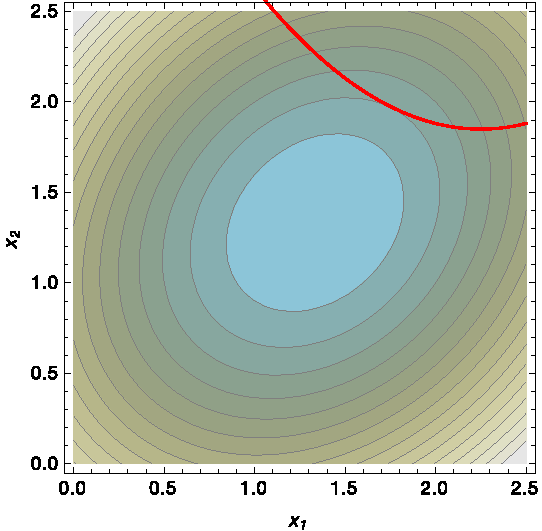
\includegraphics[width=4in]{opt_fig}
  \end{center}
  \caption{A contour plot of the function $f_0 (x_1,x_2) = (x_1 - 1)^2 + (x_2 - 1)^2 - x_1 x_2 /2$ whose minimum occurs at $(4/3,4/3)$ (i.e., the center of the blue ellipse).  The red line indicates the inequality constraint $f_1 (x_1,x_2)= 1.85 + (x_1 - 2.25)^2 / 2 - x_2 \leq 0$. The picture shows that the constrained minimum occurs where the objective contour line is tangent to the active constraint line.}
\end{figure}

The geometric picture implied by Theorem~\ref{theorem:KKT} is that of a game where one would like to decrease the objective $f_0 (\vecnot{x}^*)$ by choosing $\vecnot{y}$ such that $\nabla f_0 (\vecnot{x}^*)^T \vecnot{y}  < 0$ but there are  constraints on the set of allowable $\vecnot{y}$'s.
Let $H = \Span ( \{ \nabla h_j (\vecnot{x}^*) \})$ be the subspace of directions that violate the equality constraints at $\vecnot{x}^*$.
Similarly, let the cone of directions that violate the active inequality constraints is given by
\[ F = \left\{ \sum_{i\in A} \lambda_i \nabla f_i (\vecnot{x}^*) \, \middle| \, \lambda_i \geq 0, i \in A   \right\}. \]
Thus, one can only pick directions $\vecnot{y}$ that are orthogonal to all vectors in $H$ and also have a non-positive inner product with all vectors in $F$.

Let the matrix $P$ define the orthogonal projection of $\mathbb{R}^n$ onto $H^\perp$.
Using this, we can translate the equation~\eqref{eq:KKT1} into the statement
\[ -P \nabla f_0 (\vecnot{x}^*) \in P F \]  or ``the projection, onto $H^\perp$, of the descent direction  lies in the projection, onto $H^\perp$, of the cone of directions that violate the inequality constraints''.
The reason for this is that we can absorb the $\nabla h_j$ terms into the $\nabla f_i$ terms by defining
\[ \vecnot{f}^{(i)} = \nabla f_i (\vecnot{x}^*) + \sum_{j=1}^p \nu_{j,i} \nabla h_j (\vecnot{x}^*) = P \nabla f_i (\vecnot{x}^*) \]
so that $\vecnot{f}^{(i)} \in H^{\perp}$ for $i=0,1,\ldots,m$.
Then, the cone $PF$ is defined by
\[ PF = \left\{ \sum_{i\in A} \lambda_i \vecnot{f}^{(i)} \, \middle| \, \lambda_i \geq 0, i\in A \right\}. \]

If $-P \nabla f_0 (\vecnot{x}^*) \notin P F$, then we project $-P \nabla f_0 (\vecnot{x}^*)$ onto $PF$ to get a non-zero residual $\vecnot{y}$.
The resulting vector gives a direction where the objective function decreases linearly in $t$ and the constraint violations are $o(t)$.
The challenge in making this proof precise is that, unless the equality constraints are affine, they may not be exactly satisfied for $t>0$.
In standard proofs of this result, this difficulty is overcome by using the implicit function theorem to construct an $\vecnot{x} (t)$ that starts in the direction of $\vecnot{y}$ but is perturbed slightly to remain feasible.

\begin{proof}
For simplicity, we prove only the case where $h_j (\vecnot{x}) = \vecnot{a}_j^T \vecnot{x} - \vecnot{b}$ is affine.
%and $PF$ does contain a line (i.e., $\{\alpha \vecnot{z}\,|\, \alpha \in \mathbb{R}\}$ for some $\vecnot{z}$).
First, we define 
\[ \vecnot{y} (\vecnot{\lambda},\vecnot{\nu}) = -\nabla f_0 (\vecnot{x}^*) - \sum_{i=1}^m \lambda_i \nabla f_i (\vecnot{x}^*) - \sum_{j=1}^p \nu_j \underbrace{\nabla h_j (\vecnot{x}^*)}_{\vecnot{a}_j}. \]
The vector $\vecnot{y} (\vecnot{\lambda},\vecnot{\nu})$ can be seen as the residual of the descent direction for the objective function after the constraint gradients have been used to cancel some parts.
Next, we let $\vecnot{\nu}^* (\vecnot{\lambda}) = \arg \min_{\vecnot{\nu}\in \mathbb{R}^p} \| \vecnot{y} (\vecnot{\lambda},\vecnot{\nu}) \|$
and apply the best approximation theorem (for the standard inner product space) to see that
\[ \vecnot{y} (\vecnot{\lambda},\vecnot{\nu}^* (\vecnot{\lambda})) = P \vecnot{y} (\vecnot{\lambda},\vecnot{0}), \]
where the matrix $P$ defines an orthogonal projection onto $H^\perp$ and $H = \Span ( \{ \vecnot{a}_j \} )$.
This ensures that each $h_j ( \vecnot{x}^* + t \vecnot{y} (\vecnot{\lambda},\vecnot{\nu}^* (\vecnot{\lambda})) )=0$ for all $\vecnot{\lambda}\in \mathbb{R}^m$ and $t\in \mathbb{R}$.

Continuing, we let $S = \{ \vecnot{\lambda} \in \mathbb{R}^m \, | \, \vecnot{\lambda} \geq \vecnot{0}, \lambda_i = 0, i \notin A \}$ and compute \[\vecnot{y}^* = \arg \min_{\vecnot{\lambda} \in S} \| \vecnot{y} (\vecnot{\lambda},\vecnot{\nu}^* (\vecnot{\lambda})) \|. \]
This optimization uses the gradients of the active constraints to cancel as much of the residual descent direction as possible.
Thus, $\vecnot{y}^* \neq \vecnot{0}$ implies there is a descent direction that does not violate the constraints.
Looking at the formulas for $\vecnot{y} (\vecnot{\lambda},\vecnot{\nu})$ and $\vecnot{y} (\vecnot{\lambda},\vecnot{\nu}^* (\vecnot{\lambda}))$, we can also interpret $\vecnot{y}^*$ as the error vector for the projection of $\vecnot{v} = -P\nabla f_0 (\vecnot{x}^*)$ onto the convex set $PF$, which is the closed convex cone of perturbations that preserve the equality constraints but locally violate the inequality constraints.
Then, $\vecnot{u}^* = \vecnot{v} - \vecnot{y}^*$ equals the projection itself and we observe that Theorem~\ref{theorem:convex_proj_lt0} implies $(\vecnot{u} - \vecnot{u}^*)^T (\vecnot{v} - \vecnot{u}^*) \leq 0$ for all $\vecnot{u} \in PF$.
Since $\vecnot{0} \in PF$, we can choose $\vecnot{u} = \vecnot{0}$ to see that $(\vecnot{u}^*)^T (\vecnot{v} - \vecnot{u}^*) \geq 0$.
Using this, we can write
\begin{align*}
-(P\nabla f_0 (\vecnot{x}^*))^T \vecnot{y}^*
&= \vecnot{v}^T ( \vecnot{v} - \vecnot{u}^*) \\
&= (\vecnot{v} - \vecnot{u}^*)^T (\vecnot{v} - \vecnot{u}^*) + (\vecnot{u}^*)^T (\vecnot{v} - \vecnot{u}^*) \\
&\geq \|\vecnot{y}^*\|^2.
\end{align*}
If~\eqref{eq:KKT1} cannot be satisfied by some $\vecnot{\lambda} \in S$ and $\vecnot{\nu} \in \mathbb{R}^p$, then $\vecnot{y}^* \neq \vecnot{0}$ and $\| \vecnot{y}^* \| > 0$.
Thus, a perturbation in the $\vecnot{y}^*$ direction will decrease the value of the objective function while essentially preserving feasibility.

But, the $\vecnot{y}^*$ direction is only guaranteed to preserve feasibility to first order (i.e., $(P \nabla f_i (\vecnot{x}^*))^T \vecnot{y}^*  \leq 0$) for $i = 1,\ldots,m$.
To fix this, first one needs to augment $\vecnot{y}^*$ with a small amount of some vector $\vecnot{w}$ satisfying $(P \nabla f_i (\vecnot{x}^*))^T \vecnot{w} < 0$ for all $i = 1,\ldots,m$.
Such a vector is guaranteed by the constraint qualification.
%Such a $\vecnot{w}$ lies in the ``interior of the polar cone of $PF$'' and will exist as long as $PF$ does not contain a line.
Then, we can choose some $\delta>0$ such that $(P\nabla f_0 (\vecnot{x}^*))^T (\vecnot{y}^*+\delta \vecnot{w}) \leq -\frac{1}{2} \|\vecnot{y}^* \|$. With this modification, the definition of the derivative implies that, for sufficiently small $t$, $\vecnot{x}(t) = \vecnot{x}^* + t (\vecnot{y}^* + \delta \vecnot{w})$ will be a feasible vector satisfying $f_0 (\vecnot{x}(t)) < f_0 (\vecnot{x}^*)$.
\end{proof}

\subsection{Lagrangian Duality}


\begin{definition}
The \defn{optimization}{Lagrangian dual} function is defined to be
\[ g(\vecnot{\lambda},\vecnot{\nu}) \triangleq \inf_{\vecnot{x}\in \mathcal{D}} L(\vecnot{x},\vecnot{\lambda},\vecnot{\nu}). \]
\end{definition}


\begin{lemma}
The Lagrangian dual problem
\begin{align*}
\mathrm{maximize} \quad & g(\vecnot{\lambda},\vecnot{\nu}) \\
\mathrm{subject\,to} \quad & \vecnot{\lambda} \geq 0
\end{align*}
has a unique maximum value $d^* \leq p^*$.
This property is known as \defn{optimization}{weak duality}.
\end{lemma}

\begin{proof}
The Lagrangian dual function is concave because it is the pointwise infimum of affine functions
\begin{align*}
g(\alpha\vecnot{\lambda}+&(1-\alpha)\vecnot{\lambda}',\alpha\vecnot{\nu}+(1-\alpha)\vecnot{\nu}') \\
&= \inf_{\vecnot{x}\in \mathcal{D}} L(\vecnot{x},\alpha\vecnot{\lambda}+(1-\alpha)\vecnot{\lambda}',\alpha\vecnot{\nu}+(1-\alpha) \vecnot{\nu}') \\
&= \inf_{\vecnot{x}\in \mathcal{D}} \big( \alpha L(\vecnot{x},\vecnot{\lambda},\vecnot{\nu}) + (1-\alpha) L(\vecnot{x},\vecnot{\lambda}',\vecnot{\nu}') \big) \\
&\geq \inf_{\vecnot{x}\in \mathcal{D}} \alpha L(\vecnot{x},\vecnot{\lambda},\vecnot{\nu}) + \inf_{\vecnot{x}'\in \mathcal{D}} (1-\alpha) L(\vecnot{x}',\vecnot{\lambda}',\vecnot{\nu}') \\
&= \alpha g(\vecnot{\lambda},\vecnot{\nu}) + (1-\alpha) g(\vecnot{\lambda}',\vecnot{\nu}').
\end{align*}
Thus, it follows from Theorem~\ref{theorem:convex_unique_min} that $g$ has a unique maximum value $d^*$ which can be upper bounded by
\begin{align*}
g(\vecnot{\lambda},\vecnot{\nu})
&= \inf_{\vecnot{x}\in \mathcal{D}} L(\vecnot{x},\vecnot{\lambda},\vecnot{\nu})
\stackrel{(a)}{\leq} \inf_{\vecnot{x}\in \mathcal{F}} L(\vecnot{x},\vecnot{\lambda},\vecnot{\nu}) \\
&\stackrel{(b)}{=} p^* + \sum_{i=1}^m \lambda_i f_i (\vecnot{x})
\stackrel{(c)}{\leq} p^*,
\end{align*}
where $(a)$ is implied by $\mathcal{F} \subseteq \mathcal{D}$, $(b)$ follows from $h_j(\vecnot{x}) = 0$ for $\vecnot{x}\in \mathcal{F}$, and $(c)$ holds by combining $f_i(\vecnot{x}) \leq 0$ for $\vecnot{x}\in \mathcal{F}$ and $\lambda_i \geq 0$.
\end{proof}

The Lagrangian dual function can be $-\infty$ for a wide range of $(\vecnot{\lambda},\vecnot{\nu})$.
In this case, it makes sense to eliminate these points by defining the implicit constraint set
\begin{align*}
\mathcal{C} &\triangleq \left\{ (\vecnot{\lambda},\vecnot{\nu}) \in \mathbb{R}^m \times \mathbb{R}^p | \vecnot{\lambda}\succeq \vecnot{0},  g(\vecnot{\lambda},\vecnot{\nu}) > -\infty \right\}.
\end{align*}
The points $(\vecnot{\lambda},\vecnot{\nu}) \in \mathcal{C}$ are called \textbf{dual feasible} and it follows that
\[ d^* = \sup_{(\vecnot{\lambda},\vecnot{\nu})\in \mathcal{C}} g(\vecnot{\lambda},\vecnot{\nu}). \]
By convention, $d^* = -\infty$ if the dual problem is not feasible (i.e., $\mathcal{C} = \emptyset$).

\begin{definition}
If $d^* = p^*$, then one says \defn{optimization}{strong duality} holds for the problem.
\end{definition}

\begin{theorem}
Let $\vecnot{x}^*$ be a primal optimal point and $(\vecnot{\lambda}^*,\vecnot{\nu}^*)$ be a dual optimal point.
If strong duality holds, $\vecnot{x}^* \in \Interior{\mathcal{D}}$, and all $f_i$ and $g_j$ functions are differentiable at $\vecnot{x}^*$, then we get the KKT conditions of complementary slackness, $\lambda_i^* f_i (\vecnot{x}^*) = 0$ for $i = 1,\ldots,m$, and stationarity \eqref{eq:KKT1}.
\end{theorem}
\begin{proof}
By weak duality, we have
\[ d^* = g(\vecnot{\lambda}^*,\vecnot{\nu}^*) \leq f_0 (\vecnot{x}^*) = p^*. \]
Since $\vecnot{x}^*$ is feasible, combining $d^* = p^*$ with the proof of weak duality shows that
\[ \inf_{\vecnot{x}\in \mathcal{D}} L(\vecnot{x},\vecnot{\lambda}^*,\vecnot{\nu}^*) = L(\vecnot{x}^*,\vecnot{\lambda}^*,\vecnot{\nu}^*) \]
and $\lambda_i^* = 0$ if the $i$-th inequality constraint is inactive (i.e., $f_i(\vecnot{x}^*) < 0$).
Thus, we also observe that complementary slackness condition $\lambda_i^* f_i (\vecnot{x}^*) = 0$ holds for $i = 1,\ldots,m$.
Since $\vecnot{x}^* \in \Interior{\mathcal{D}}$, it follows that $\vecnot{x}^*$ is a locally optimal point of $L(\vecnot{x},\vecnot{\lambda}^*,\vecnot{\nu}^*)$.
Thus, $\vecnot{x}^*$ must be a stationary point of $L(\vecnot{x},\vecnot{\lambda}^*,\vecnot{\nu}^*)$ and taking the $\vecnot{x}$-derivative gives~\eqref{eq:KKT1}.
\end{proof}

\begin{example}
For the first LP in Definition~\ref{def:standard_lp}, the Lagrangian is given by
	\[ L(\vecnot{x},\vecnot{\lambda},\vecnot{\nu}) = \vecnot{c}^T \vecnot{x} + \vecnot{\nu}^T (\vecnot{b} - A\vecnot{x}) - \vecnot{\lambda}^T \vecnot{x}, \]
	where the $\vecnot{\lambda}$ term is negative because the constraint is $\vecnot{x} \succeq \vecnot{0}$.
Thus, the Lagrangian dual function is given by
\begin{equation*}
g(\vecnot{\lambda},\vecnot{\nu})
= \inf_{\vecnot{x}\in \mathcal{D}} L(\vecnot{x},\vecnot{\lambda},\vecnot{\nu})
	= \begin{cases} \vecnot{b}^T \vecnot{\nu} & \text{if } \vecnot{c} - A^T \vecnot{\nu} - \vecnot{\lambda} = \vecnot{0} \\
-\infty & \text{otherwise}. \end{cases}
\end{equation*}
Solving the implicit constraint and using the fact that $\vecnot{\lambda} \succeq \vecnot{0}$, one gets the dual LP problem
\begin{align*}
\mathrm{maximize} \quad & \vecnot{b}^T \vecnot{\nu} \\
	\mathrm{subject\,to} \quad & A^T \vecnot{\nu} \preceq \vecnot{c}.
\end{align*}
Strong duality for linear programs says that, if the original LP has an optimal solution (i.e., it is neither unbounded nor infeasible), then the dual LP has an optimal solution of the same value.
\end{example}

\subsection{Convex Optimization}

\begin{definition} \label{def:convex_opt}
An optimization problem in standard form is called \defn{optimization}{convex} if all $f_i$ functions are convex, all the $h_j$ functions are affine (i.e., $h_j(\vecnot{x}) = \vecnot{a}_j^T \vecnot{x} - b_j)$, and $\mathcal{D}=\RealNumbers^n$. 
\end{definition}

\begin{problem}
For a convex standard-form optimization problem (i.e.,  satisfying Definition~\ref{def:convex_opt}), show that the feasible set is a convex set.
\end{problem}

Applying Theorem~\ref{theorem:convex_unique_min} to this setup shows that a convex standard-form optimization problem has a unique minimum value.
Also, if the function $f_0$ is strictly convex, then the minimum value achieved uniquely.
There are a number of stronger conditions that also imply strong duality for convex optimization problems.
\defn{optimization}{Slater's condition} is stated below as a theorem and its proof can be found in~\cite[Sec.~5.3.2]{Boyd-2004}.
 
\begin{theorem}[Slater's Condition]
If a convex optimization problem has a point $\vecnot{x}_0$ where $f_i(\vecnot{x}_0) < 0$ for $i=1,\ldots,m$ and $h_j (\vecnot{x}_0) = 0$ for $j=1,\ldots,p$, then the MF constraint qualification and strong duality both hold for the problem.
In addition, if all $f_i$ functions are differentiable, then the KKT conditions are necessary and sufficient for optimality.
\end{theorem}


\begin{example}
For a channel with colored noise, the input distribution that maximizes the achievable information rate can be found by solving the convex optimization problem, known as water-filling, given by
\begin{align*}
\mathrm{minimize} \quad & -\sum_{i=1}^n \log \left( x_i + \alpha_i \right) \\
\mathrm{subject\,to} \quad & \sum_{i=1}^n x_i = P \\
& \vecnot{x} \succeq 0.
\end{align*}
Choosing $x_i = \frac{P}{n}$ for $i=1,\ldots,n$ gives a point that satisfies Slater's condition, so strong duality holds for this problem.
\end{example}

\begin{example}
For the water-filling problem, the Lagrangian can be written as
\[ L(\vecnot{x},\vecnot{\lambda},\nu) = - \sum_{i=1}^n \log(x_i + \alpha_i) - \sum_{i=1}^m \lambda_i x_i + \nu \left( -P + \sum_{i=1}^n x_i \right)  \]
and the Lagrangian dual is given by $g(\vecnot{\lambda},\nu)
= \inf_{\vecnot{x}\in \mathbb{R}^n} L(\vecnot{x},\vecnot{\lambda},\nu)$.

If $\lambda_i <0$, then the Lagrangian tends to $-\infty$ as $x_i \to -\infty$.
Thus, the system is implicitly constrained to have $\lambda_i \geq 0$.
The first-order optimality conditions, for $i=1,2,\ldots,n$, are given by
\[ -\frac{1}{x_i + \alpha_i} - \lambda_i + \nu = 0.
\]
Solving this for $x_i$ shows that $x_i$ is increasing in $\lambda _i$ (for $\lambda_i \geq 0$) and this implies that $g(\vecnot{\lambda},\nu)$ is decreasing in $\lambda_i$ (for $\lambda_i \geq 0$ and $x_i \geq 0$).

Thus, the expression
$\max_{\vecnot{\lambda} \geq 0} g(\vecnot{\lambda},\nu)$
is given by choosing the smallest non-negative $\lambda_i$'s for which $x_i \geq 0$.
This implies that
\[ (x_i,\lambda_i) = \begin{cases} \left( \frac{1}{\nu} - \alpha _i, 0 \right) & \text{if }\nu < \frac{1}{\alpha_i} \\ \left(0,\nu-\frac{1}{\alpha_i}\right) & \text{if } \nu \geq \frac{1}{\alpha_i}. \end{cases} \]
From this, the value of $\nu$ can be determined by solving
\[\sum_{i=1}^n x_i = \sum_{i=1}^n \max \left\{ 0,\frac{1}{\nu}-\alpha_i \right\} = P. \]
By strong duality, the optimal value of the dual problem equals the optimal value of the original problem.
Finally, the problem can be easily solved for a range of $P$ values by sweeping through a range of $\nu$ values and computing $P$ in terms of $\nu$.
\end{example}

\appendix
\chapter{Optional Topics}

\section{Dealing with Infinity*}

\subsection{The Axiom of Choice}

The \defn{set theory}{axiom of choice}, formulated by Zermelo in 1904, is innocent-looking.
However, one can prove theorems with its aid that some mathematicians were originally reluctant to accept in the past.

\begin{definition}[The Axiom of Choice]
Given a collection $\mathcal{X}$ of disjoint nonempty sets, there exists a set $C$ having exactly one element in common with each element of $\mathcal{X}$.
That is, for each $X \in \mathcal{X}$ the set $C \cap X$ contains a single element.
\end{definition}

Most mathematicians today accept the axiom of choice as part of the set theory on which they base their mathematics.
A straightforward consequence of the axiom of choice is the existence of a choice function.

\begin{lemma}[Existence of a Choice Function]
Given a collection $\mathcal{Y}$ of non-empty sets, there exists a function
\begin{equation*}
c: \mathcal{Y}  \rightarrow \bigcup_{Y \in \mathcal{Y}} Y
\end{equation*}
satisfying $c(Y) \in Y$ for every $Y \in \mathcal{Y}$.
\end{lemma}
\begin{proof}
The difference between the axiom of choice and the lemma is that in the latter statement the sets of the collection $\mathcal{Y}$ need not be disjoint.
Given an element $Y \in \mathcal{Y}$, define the set $Y'$ by
\begin{equation*}
Y' = \left\{ \left( Y, y \right) | y \in Y \right\}.
\end{equation*}
That is, $Y'$ is the collection of all ordered pairs where the first coordinate of the ordered pair is the set $Y$, and the second coordinate is an element of $Y$.
Because $Y$ contains at least one element, the set $Y'$ is nonempty.
Furthermore, $Y'$ is a subset of the cartesian product
\begin{equation*}
\mathcal{Y} \times \bigcup_{Y \in \mathcal{Y}} Y.
\end{equation*}
If $Y_1$ and $Y_2$ are two different sets in $\mathcal{Y}$, then the sets $Y_1'$ and $Y_2'$ are disjoint; specifically, the elements of $Y_1'$ and $Y_2'$ differ at least in their first coordinates.

Consider the collection
\begin{equation*}
\mathcal{Z} = \left\{ Y' | Y \in \mathcal{Y} \right\}.
\end{equation*}
This is a collection of disjoint nonempty subsets of
\begin{equation*}
\mathcal{Y} \times \bigcup_{Y \in \mathcal{Y}} Y.
\end{equation*}
By the axiom of choice, there exists a set $Z$ having exactly one element in common with each element of $\mathcal{Z}$.
Define the function
\begin{equation*}
c: \mathcal{Z} \rightarrow
\mathcal{Y} \times \bigcup_{Y \in \mathcal{Y}} Y
\end{equation*}
by $c \left( Y' \right) = Y' \cap Z$.
This function $c$ implicitly provides the rule for a function from $\mathcal{Y}$ to the set $\bigcup_{Y \in \mathcal{Y}} Y$ such that $y$ belongs to $Y$ whenever $\left( Y, y \right) \in Z$.
This rule is the desired choice function.
\end{proof}


\subsection{Well-Ordered Sets}

A \defn{set theory}{simple order $<$} on a set $X$ is a relation such that, for all $x, y, z \in X$,
\begin{enumerate}
\item if $x \neq y$ then either $x < y$ or $y < x$
\item if $x < y$ then $x \neq y$
\item if $x < y$ and $y < z$ then $x < z$.
\end{enumerate}

\begin{definition}
A set $X$ with an order relation $<$ is said to be \defn{set theory}{well-ordered} if every nonempty subset of $X$ has a smallest element.
\end{definition}

The set of natural numbers, for example, is well-ordered.
On the other hand, the set of integers is not well-ordered.

\begin{fact}[Well-ordering theorem]
If $X$ is a set, there exists an order relation on $X$ that is a well-ordering.
\end{fact}

This theorem was proved by Zermelo using the axiom of choice.
It startled the mathematical community in 1904 and spurred much controversy about the axiom of choice.
It is given here without a proof.

\begin{corollary}
There exists an uncountable well-ordered set.
\end{corollary}

\begin{definition}
Let $X$ be an ordered set.
Given $x \in X$, the set
\begin{equation*}
Y_x = \left\{ y \in Y | y < x \right\}
\end{equation*}
is called the \textbf{section} of $X$ by $x$.
\end{definition}

\begin{corollary}
There exists an uncountable well-ordered set, every section of which is countable.
\end{corollary}

The well-ordering principle is a necessary tool in proofs by induction when the set over which the induction process is applied is not a segment of the natural numbers; this is the so-called transfinite induction.


\subsection{The Maximum Principle}

A \defn{set theory}{strict partial order} $\prec$ on a set $X$ is a relation such that for all $x, y, z \in X$
\begin{enumerate}
\item if $x \prec y$ then $x \neq y$
\item if $x \prec y$ and $y \prec z$ then $x \prec z$.
\end{enumerate}

A strict partial order is similar to a simple order, except that it need not be true that for every distinct $x, y \in X$, either $x \prec y$ or $y \prec x$.

\begin{fact}[The maximum principle]
Let $X$ be a set and suppose that $\prec$ is a strict partial order on $X$.
If $Y$ is a subset of $X$ that is simply ordered by $\prec$, then there exists a maximal simply ordered subset $Z$ of $X$ containing $Y$.
\end{fact}

The maximum principle is given here without a proof.
It is interesting to note that the well-ordering theorem and the maximum principle are equivalent; either of them implies the other.
Furthermore, each of them is equivalent to the axiom of choice.

Let $\prec$ be a strict partial order on $X$.
For $x, y \in X$, the relation $x \preceq y$ holds if $x \prec y$ or $x = y$.
The relation $\preceq$ so defined is called a \defn{set theory}{partial order} on $X$.
For example, the inclusion relation $\subset$ on a collection of sets is a partial order, whereas proper inclusion is a strict partial order.


%\chapter{Solutions}

\noindent
\textbf{S~\ref{problem:RationalNumbers}}.
For every $\frac{m}{n}, \frac{p}{q} \in \RationalNumbers$, we have
\begin{gather*}
\frac{m}{n} + \frac{p}{q} = \frac{mq + np}{nq} \in \RationalNumbers \\
\frac{m}{n} \frac{p}{q} = \frac{mp}{nq} \in \RationalNumbers .
\end{gather*}
For $m \neq 0$, $\left( \frac{m}{n} \right)^{-1} = \frac{n}{m} \in \RationalNumbers$.
The remaining properties are straightforward to prove.




\backmatter 

\printindex

\end{document}

